% !TeX program = xelatex
\documentclass{article}
\usepackage[paperwidth=155mm,paperheight=230mm,margin=18mm]{geometry}
\usepackage{fontspec,xeCJK,graphicx,xcolor,tikz}
\usepackage[absolute,overlay]{textpos}
\usepackage[unicode,pdfpagelayout=TwoPageLeft,pdftitle={阿尔刻提斯之歌 · 中英对照剧本}]{hyperref}
\setmainfont{texgyrepagella-regular.otf}[
  ItalicFont=texgyrepagella-italic.otf,
  BoldFont=texgyrepagella-bold.otf,
  BoldItalicFont=texgyrepagella-bolditalic.otf]
\IfFileExists{/usr/local/share/fonts/f/FZShuSong_Z01_Regular.ttf}{
  \setCJKmainfont{FZShuSong_Z01_Regular.ttf}[Path=/usr/local/share/fonts/f/,ItalicFont=FZKai_Z03_Regular.ttf]
  \newCJKfontfamily\kai{FZKai_Z03_Regular.ttf}[Path=/usr/local/share/fonts/f/]
  \newCJKfontfamily\hei{FZHei_B01_Regular.ttf}[Path=/usr/local/share/fonts/f/]
}{
  \setCJKmainfont{Noto Serif CJK SC}
  \newCJKfontfamily\kai{FangSong}
  \newCJKfontfamily\hei{Noto Sans CJK SC}
}
\definecolor{ink}{gray}{.12}
\definecolor{quiet}{gray}{.40}
\pagestyle{empty}
\color{ink}
\setlength{\parindent}{0pt}
\setlength{\parskip}{0pt}
\xeCJKsetup{PunctStyle=kaiming}
\textblockorigin{0mm}{0mm}
\newcommand{\ENsetup}{\normalfont\color{ink}\fontsize{11}{16.5}\selectfont\emergencystretch=1.5em}
\newcommand{\ZHsetup}{\normalfont\color{ink}\fontsize{10.5}{17}\selectfont\emergencystretch=1.5em}
\newcommand{\ENspeaker}[1]{{\fontsize{9.8}{13}\selectfont\scshape\bfseries #1}\par\vspace{3pt}}
\newcommand{\ZHspeaker}[1]{{\hei\fontsize{10.3}{13}\selectfont #1}\par\vspace{3pt}}
\newcommand{\ENstage}[1]{\par\noindent{\itshape #1}\par}
\newcommand{\Note}[2]{\par\hangindent=1.5em\hangafter=1\noindent\makebox[1.5em][l]{#1}#2\par}
\newcommand{\Block}[3]{\begin{textblock*}{119mm}(18mm,#1mm){#2 #3\par}\end{textblock*}}
\newcommand{\Heading}[3]{%
  \begin{textblock*}{119mm}(18mm,12mm)
    \color{quiet}\fontsize{7.5}{10}\selectfont
    #1\hfill #2\par\vspace{3mm}\hrule height .2pt
  \end{textblock*}
  \begin{textblock*}{119mm}(18mm,214mm)
    \color{quiet}\fontsize{7}{10}\selectfont #3\hfill\thepage
  \end{textblock*}
}
\newcommand{\Ornament}{%
  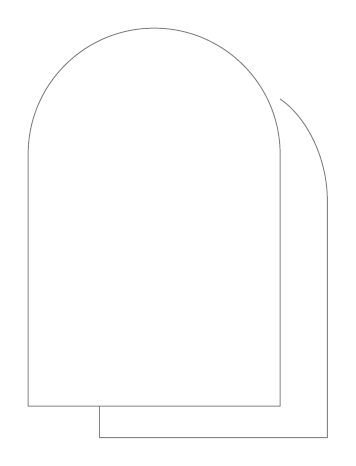
\begin{tikzpicture}[x=1mm,y=1mm,draw=ink!55,line width=.35pt]
    \draw (9,0)--(38,0)--(38,30).. controls (38,36) and (35,41)..(32,43);
    \draw (9,0)--(9,4);
    \draw (0,4)--(32,4)--(32,36) arc[start angle=0,end angle=180,radius=16]--cycle;
  \end{tikzpicture}
}

\begin{document}
\null
\begin{textblock*}{119mm}(18mm,40mm)\centering \fontsize{25}{35}\selectfont THE\\ALCESTIAD\end{textblock*}
\begin{textblock*}{119mm}(18mm,74mm)\centering\fontsize{10}{15}\selectfont THORNTON WILDER\end{textblock*}
\begin{textblock*}{119mm}(18mm,100mm)\centering\fontsize{13}{20}\selectfont FOREWORD · ACTS I–III · THE DRUNKEN SISTERS\par\vspace{13mm}\Ornament\end{textblock*}
\begin{textblock*}{109mm}(23mm,185mm)\centering\fontsize{10}{15}\selectfont The rear court of the palace of Admetus, King of Thessaly, many centuries before the Great Age of Greece.\end{textblock*}
\begin{textblock*}{119mm}(18mm,215mm)\centering\color{quiet}\fontsize{8}{11}\selectfont ENGLISH · CHINESE\end{textblock*}
\newpage
\null
\begin{textblock*}{119mm}(18mm,48mm)\centering \fontsize{23}{34}\selectfont 阿尔刻提斯之歌\end{textblock*}
\begin{textblock*}{119mm}(18mm,74mm)\centering\fontsize{10}{15}\selectfont 桑顿·怀尔德\end{textblock*}
\begin{textblock*}{119mm}(18mm,100mm)\centering\fontsize{13}{20}\selectfont 前言 · 第一幕 · 第二幕 · 第三幕 · 醉酒的女神\par\vspace{13mm}\Ornament\end{textblock*}
\begin{textblock*}{109mm}(23mm,185mm)\centering\fontsize{10}{15}\selectfont 塞萨利国王阿德墨托斯王宫的后院，\\希腊黄金时代几个世纪之前。\end{textblock*}
\begin{textblock*}{119mm}(18mm,215mm)\centering\color{quiet}\fontsize{8}{11}\selectfont 中英对照 · 节选\end{textblock*}
\newpage
\null
\Heading{THE ALCESTIAD}{FOREWORD}{Original p. ix}
% foreword-0 en
\Block{30.000}{\ENsetup}{On the last pages of Thornton Wilder's novel \textit{The Eighth Day}, my brother has one of the leading characters refute the usual image of the life experience as a river flowing onward between defined banks. Instead, the human adventure is described as a tapestry with indeterminate breadth as well as length and the individual pattern visible on both sides of the fabric. The story is outlined in colored yarn, the design perhaps wildly asymmetrical but nevertheless clear, truthful, complete. A record and a portrait.\par}
% foreword-1 en
\Block{79.514}{\ENsetup}{Thornton's tapestry was minute when at the age of seven or eight in Madison, Wisconsin, he first heard the name Alcestis while reading or being read to from Bulfinch's \textit{The Age of Fable}. The story of the daughter of King Pelias, princess of princesses in the myth and the song of pre-Christian Greece, captured his imagination—and his heart. The thread of her white yarn was knotted into his bit of fabric and she became a benign insistence in his inner consciousness, that hidden storehouse which is an author's source and springboard. She was the haunting shadow of a play that would take years to write.\par}
\newpage
\null
\Heading{阿尔刻提斯之歌}{前言}{原书 1–2}
% foreword-0 zh
\Block{30.000}{\ZHsetup}{人们总是将生命看作一条沿着既定路线奔流的河，而在桑顿·怀尔德的小说《第八日》的最后几页，我哥哥让其中一位主角反驳了这种看法。相较之下，一个人的人生经历就像一张织毯，它的长和宽都不确定，两面的纹路也不尽相同。彩色的纱线勾勒出故事的轮廓，设计上也许极不对称，却清晰、真实而完整。是记录，也是肖像。\par }
% foreword-1 zh
\Block{79.514}{\ZHsetup}{桑顿的命运织毯起初还很小，七八岁时他生活在威斯康星州的麦迪逊市，在阅读布尔凡奇的《寓言时代》时第一次听到了阿尔刻提斯这个名字。在前基督教时期的希腊神话和歌谣中，国王佩利阿斯的女儿是公主中的公主。她的故事占据了他的想象，也俘获了他的心灵。她的白色纱线嵌进了他的命运织物中，阿尔刻提斯成为他潜意识中一份温柔的坚持，一个有待发掘的灵感素材。她是一个戏剧雏形，直到多年后才得以创作出来。\par }
\newpage
\null
\Heading{THE ALCESTIAD}{FOREWORD}{Original pp. ix–x}
% foreword-2 en
\Block{30.000}{\ENsetup}{The knot in Alcestis's thread was tied when the Wilder family moved to Berkeley, California, where the magnificent Greek Theater built into the hillside of a eucalyptus grove was a new and lively part of the life of the university and the town. Several times a year the Classics Department mounted productions of plays by Sophocles, Aeschylus, and Euripides. Our mother joined the volunteer workers in the costume shop and stenciled furlongs of borders in the Greek key or laurel leaf patterns on gorgeously colored togas. She made a little blue one with shells around the hem for Thornton—and a green one for brother Amos—and sent them off to apply for roles as members of the Athenean mob. Thus Thornton discovered ``total'' theater and the Golden Age of Antiquity. His experience until then had been a performance of \textit{As You Like It} seen from the top gallery of a Milwaukee theater.\par}
% foreword-3 en
\Block{108.498}{\ENsetup}{By now Thornton was ten; black-haired, blue-eyed, acquisitive and radiant. Even before this he had claimed his share of a writer's allotment of the twenty-six letters of the alphabet and had begun to tame them into a vocabulary that would allow him—in good time—to speak in his own way. He went to bed early and got up early to write, and the full range of his enlarging vocabulary was turned to inventing dialogue. He draped us and the neighbors' children in yards of begged or borrowed cheesecloth and coaxed us into declaiming his grandiloquent speeches.\par}
% foreword-4 en
\Block{163.783}{\ENsetup}{Four years later he was a boarding pupil in the China Inland Mission School in Chefoo. Studies in the classics began early in a British school preparing its pupils for the Oxford-Cambridge Examinations.\par}
\newpage
\null
\Heading{阿尔刻提斯之歌}{前言}{原书 2–3}
% foreword-2 zh
\Block{30.000}{\ZHsetup}{当怀尔德一家搬到加利福尼亚州伯克利时，阿尔刻提斯之线打了个结。桉树林山坡上建有一座宏伟的希腊剧院，是学校和小镇生活中生机勃勃的一部分。古典学系每年都会制作几部索福克勒斯、埃斯库罗斯和欧里庇得斯的戏剧作品。我们的母亲参与了服装组的志愿工作，用模板印出希腊钥匙的形状，或是在漂亮的长袍上印上月桂树叶的图案。她给桑顿做了一件有贝壳镶边的蓝色小袍子——给哥哥阿莫斯做了一件绿色的——然后让他们去扮演雅典民众。桑顿就这样了解到了“整个”剧场和古希腊的黄金时代，在这之前，他的全部剧场经验不过是坐在密尔沃基剧院的后排看了一场《皆大欢喜》。\par }
% foreword-3 zh
\Block{108.498}{\ZHsetup}{桑顿十岁了，黑头发，蓝眼睛，充满好奇心，精力旺盛。早在十岁之前他就掌握了作家们的工具，驯服了二十六个字母为自己服务，将它们组成词汇，在适当的时候用来表达自己。他早睡早起写作，随着词汇量的增长，他开始创造对话。他给我们和邻居的孩子披上借来的纱，哄着我们一起朗诵他的豪言壮语。\par }
% foreword-4 zh
\Block{163.783}{\ZHsetup}{四年之后，他成为中国烟台一所教会学校的寄宿生。在一所英国人开办的专为牛津、剑桥入学考试做准备的学校里，他开始了对古典文学的学习。\par }
\newpage
\null
\Heading{THE ALCESTIAD}{FOREWORD}{Original pp. x–xi}
% foreword-5 en
\Block{30.000}{\ENsetup}{The first half of his undergraduate years was spent at Oberlin College in Ohio, where he became a privileged student and friend of a great teacher who was also a distinguished classicist—Professor Charles H. A. Wager. Alcestis's thread wove a visibly increasing pattern during these years and later, following his graduation from Yale in 1920, when he spent eight months at the American Academy for Classical Studies in Rome. Not qualified as a Graduate Fellow, he nevertheless audited lectures, went on digs with the archaeologists and pored over fragile papyri. In the museums and art galleries of Italy he caught Alcestis's shadow.\par}
% foreword-6 en
\Block{90.084}{\ENsetup}{In the decades of the twenties and the thirties the tapestry grew in size and density. The design was of teaching—first French at The Lawrenceville School and then comparative literature, including the Greek dramatists, at the University of Chicago—and lecture tours and script-writing in Hollywood. He published two volumes of short plays and four novels. One, \textit{The Bridge of San Luis Rey}, brought him the first of three Pulitzer Prizes and, at the age of thirty, world-wide fame weighted with a cumbersome bag of perquisites: honors, privileges, dazzling opportunities balanced by loss of privacy and hazards to body, mind, and spirit.\par}
% foreword-7 en
\Block{151.184}{\ENsetup}{During these years the first of Thornton's long plays, \textit{Our Town}, was produced to immediate success, and the second, \textit{The Merchant of Yonkers}, to failure. André Obey's play, \textit{Lucrèce}, which Katharine Cornell had commissioned my brother to translate for her, opened and closed while Ibsen's \textit{A Doll's House}, adapted by him for Ruth Gordon, was a conspicuous success.\par}
\newpage
\null
\Heading{阿尔刻提斯之歌}{前言}{原书 3–4}
% foreword-5 zh
\Block{30.000}{\ZHsetup}{他大学时代的前两年是在俄亥俄州的欧伯林学院度过的。在那里他成了查尔斯·H. A. 瓦格教授的得意门生和朋友，而瓦格教授本身也是一名出色的古典文学家。1920 年从耶鲁大学毕业后，他在美国设立于罗马的古典学研究院待了八个月，阿尔刻提斯之线在这些年里有了更清晰的纹路。尽管不是一名研究员，他还是会去听讲座，和考古学家们一起去挖掘现场，仔细研读莎草纸上的文字。在意大利的博物馆和美术馆里，他捕捉到了阿尔刻提斯的影子。\par }
% foreword-6 zh
\Block{90.084}{\ZHsetup}{在二十世纪二三十年代里，这张命运织毯延展得更大，也变得更加密实。他开始从事教学工作——先是在劳伦斯维尔学校教授法语，然后在芝加哥大学教授比较文学，其中也会讲到古希腊的剧作家们——还有巡回演讲以及在好莱坞进行电影剧本创作。他出版了两部短剧集和四部小说，其中一部《圣路易斯雷大桥》为他赢得了普利策奖，在三十岁的这一年使他名扬四海。随之而来的是各种特权、荣誉和令人眼花缭乱的机遇，同时他也失去了很多隐私，身体、思想和精神都受到了危害。\par }
% foreword-7 zh
\Block{151.184}{\ZHsetup}{这几年里，桑顿的第一部长剧《我们的小镇》在制作演出后便取得了成功。第二部剧《扬克斯商人》则以失败告终。安德烈·奥比的剧作《卢克丽丝》由凯瑟琳·康奈尔委托给我哥哥翻译，这部剧开演后又停演。与此同时，他帮鲁斯·戈登改编的易卜生的《玩偶之家》则取得了巨大的成功。\par }
\newpage
\null
\Heading{THE ALCESTIAD}{FOREWORD}{Original pp. xi–xii}
% foreword-8 en
\Block{30.000}{\ENsetup}{In the summer of 1939 Thornton returned home wonderfully free at last of all outside commitments, with his head full of plans for his own work. He had the beginnings of two projects, both plays. One did not have a name yet. The other was \textit{The Alcestiad}. September came and Hitler's armies flooded Holland and Belgium. Thornton had no choice; \textit{The Alcestiad} was not a play for a war-torn world. The untitled project which became \textit{The Skin of Our Teeth} was.\par}
% foreword-9 en
\Block{73.676}{\ENsetup}{Soon after Pearl Harbor Thornton was commissioned a captain in the Air Force. By strange coincidence his final leave before going overseas came at the time of the previews and opening of \textit{The Skin of Our Teeth} in New York. The morning that Mother and I said goodbye to him he patted his bulging duffle bag. ``I have the manuscript of \textit{The Alcestiad} in my kit. I've been thinking how I could make it into a good one-act. It's very possible by using just the big second act scene. I'd like to leave a finished piece of work . . . might come in handy, Mother. It's a toss-up if \textit{The Skin of Our Teeth} will catch on. . . .''\par}
% foreword-10 en
\Block{128.950}{\ENsetup}{Two years later, while he was waiting in a camp near Boston to be separated from the Air Force (a lieutenant colonel now), his papers were lost. The commanding officer of the post offered a three-day pass. Thornton went straight from the Back Bay station to the Boston Public Library on Copley Square, where he drowned himself once more in the Golden Age of Greece. A few days later he was for the first time in more than three years seated at his own desk in Hamden, Connecticut.\par}
\newpage
\null
\Heading{阿尔刻提斯之歌}{前言}{原书 4–5}
% foreword-8 zh
\Block{30.000}{\ZHsetup}{1939 年夏天，桑顿终于完成了所有的邀约工作，带着完全自由的状态和满腹个人创作计划回到家中。他已经写了两部作品的开头，两部都是戏剧。一部还没有命名，另一部就是《阿尔刻提斯之歌》。九月到了，希特勒的军队横扫了荷兰和比利时，桑顿别无选择。《阿尔刻提斯之歌》并不适合一个战乱的世界。此时尚未被命名的《九死一生》才更合适。\par }
% foreword-9 zh
\Block{73.676}{\ZHsetup}{珍珠港事件后，桑顿被任命为空军上尉。很巧的是，他出国服役前的最后一天，正是《九死一生》在纽约首演的日子。我和母亲同他告别的那个早上，他拍了拍自己鼓鼓的行囊说道：“我打包了《阿尔刻提斯之歌》的手稿在里面。我一直在琢磨把它写成一个不错的独幕剧，很可能只需要第二幕的那一大场戏。我想留下一部完成的作品……说不定能派上用场，妈妈。《九死一生》能不能成功也说不定呢……”\par }
% foreword-10 zh
\Block{128.950}{\ZHsetup}{两年后，他弄丢了自己的手稿。彼时他已经是一位空军中校，正在波士顿附近的军营里等待着退伍。指挥官批准他离开三天，桑顿从后湾车站直奔科普利广场的波士顿图书馆，再次沉浸到了古希腊的黄金时代之中。几天后，他终于在三年后又一次坐在了康涅狄格汉姆登自己的书桌前。\par }
\newpage
\null
\Heading{THE ALCESTIAD}{FOREWORD}{Original pp. xii–xiii}
% foreword-11 en
\Block{30.000}{\ENsetup}{A single sheet of paper from that time is before me now. Printed on one side in big block letters is:\par}
% foreword-12 en
\Block{44.708}{\ENsetup}{\centering 
THE ALCESTIAD\par
A PLAY OF QUESTIONS\par}
% foreword-13 en
\Block{59.012}{\ENsetup}{On the reverse in his small careful penmanship is:\par}
% foreword-14 en
\Block{67.913}{\ENsetup}{\leftskip=4mm\rightskip=3mm 
(Sketches up to and including the Tiresias scene of Act One had been made before the War and lost)\par
Draft One of the first act, May and July 1945\par
Draft Two, begun July 8, 1945\par
This Draft Three begun (after completion of Act II and half of Act III) on Dec\par}
% foreword-15 en
\Block{105.728}{\ENsetup}{The unfinished date would be 1945.\par}
% foreword-16 en
\Block{114.188}{\ENsetup}{The loss of the manuscript meant more to my brother than these few notes convey; his eagerness to get back to his peacetime profession fired his enthusiasm and carried him along for the seven months of work recorded here. But, like millions of other soldiers, he had returned home not only a disoriented and exhausted man but a changed one. He was not able easily to recapture his prewar vision of Alcestis and he did not have the reserve of physical and nervous energy to sustain the excitement and tension to finish his work. He found he was beginning to destroy rather than build. Fortunately he recognized this and put the manuscript away again before doing it injury.\par}
\newpage
\null
\Heading{阿尔刻提斯之歌}{前言}{原书 5–6}
% foreword-11 zh
\Block{30.000}{\ZHsetup}{此刻我面前正放着那时他留下的一张纸，一面用大写字母打印着：\par }
% foreword-12 zh
\Block{44.708}{\ZHsetup}{\centering\kai 《阿尔刻提斯之歌》\par 一出充满问题的戏剧\par }
% foreword-13 zh
\Block{59.012}{\ZHsetup}{反面是他写的一些小字：\par }
% foreword-14 zh
\Block{67.913}{\ZHsetup}{\leftskip=4mm\rightskip=3mm\kai {\kai （第一幕戏的草稿，包括有忒瑞西阿斯的场景，都在战争前完成，已经遗失）}\par 第一幕初稿，1945 年 5 月和 7 月\par 第二稿，1945 年 7 月 8 日开始创作\par 第三稿，12 月开始{\kai （在第二幕与第三幕的一半完成后）}\par }
% foreword-15 zh
\Block{105.728}{\ZHsetup}{没写上的日期应该是 1945 年。\par }
% foreword-16 zh
\Block{114.188}{\ZHsetup}{遗失手稿给哥哥带来的影响远不是这几行笔记可以传达的。他急切地想要回到和平时期的状态中，这激发了他的热情，让他如记录中所写的样子，连续创作了七个月的时间。然而，就如同其他上百万的士兵们一样，他回到家时不只是迷茫与疲惫，整个人也完全改变了。他不再能够以战争之前那样的视角来看待阿尔刻提斯了，他的体力和精力也不足以支撑自己保持一个亢奋的状态来完成工作。他发现自己所做的更多是破坏而不是创造。好在他意识到了这一点，在造成破坏前就停止了自己的工作。\par }
\newpage
\null
\Heading{THE ALCESTIAD}{FOREWORD}{Original p. xiii}
% foreword-17 en
\Block{30.000}{\ENsetup}{Ancient literature is replete with warriors and battlefields, tyrants and heroes. My brother's thoughts were still lively with his own recent experiences of Hitler's and Mussolini's wars: one year spent on the North African coast among the ruins and ghosts of Hellenic and Roman conquest; another year in southern Italy, likewise haunted by dramatic legend, with Caesar's image triumphant. Thornton suddenly saw his next work plain. And so it happened that the novel, \textit{The Ides of March}, was written and published in 1948. It opened the way for his return to civilian life, to teaching and lecturing again, to the theater and to Alcestis.\par}
% foreword-18 en
\Block{90.084}{\ENsetup}{Thornton was only one of many authors after Euripides to be inspired to retell in his own way the Alcestis fable. Among others Christoph Martin Wieland in Germany in 1773 wrote a libretto for an operetta on the subject. In the next century the poets Richard von Hofmannstahl in Austria and Robert Browning in England used the myth. T. S. Eliot borrowed from it for an aspect of his successful play, \textit{The Cocktail Party}. And no wonder, for the theme of conjugal love and the willingness of a wife to die for her husband is an appealing and thought-provoking challenge to any author anxious to explore and praise the capabilities of humankind.\par}
\newpage
\null
\Heading{阿尔刻提斯之歌}{前言}{原书 6–7}
% foreword-17 zh
\Block{30.000}{\ZHsetup}{古代文学故事里满是战场和战士，暴君和英雄。哥哥的思绪还围绕着他自己在希特勒和墨索里尼带来的战争中的经历：他在北非待了一年，就在那些希腊与罗马帝国留下的废墟与阴影里；又在意大利南部待了一年，那里同样充满戏剧性的传说，例如恺撒的胜利。桑顿突然有了新作品的灵感，他的小说《三月十五》在 1948 年出版。这部小说开启了他回归文明世界的道路，他又开始教书，演讲，上剧场，重新思考阿尔刻提斯的故事。\par }
% foreword-18 zh
\Block{90.084}{\ZHsetup}{在欧里庇得斯之后，有许多作家想要以自己的方式改编阿尔刻提斯的故事。1773 年，克里斯托夫·马丁·维兰德以此为题创作了一部歌剧剧本。在十九世纪，奥地利诗人胡戈·冯·霍夫曼斯塔尔和英国作家罗伯特·勃朗宁也都选取过这个题材。T. S. 艾略特在他成功的剧作《鸡尾酒会》中也有所借用。也难怪，这个故事的主旨是夫妻之间的爱，以及妻子愿意为了丈夫而死。这对任何想要发掘和赞美人类能动性的作者来说，都是充满吸引力且发人深省的挑战。\par }
\newpage
\null
\Heading{THE ALCESTIAD}{FOREWORD}{Original pp. xiii–xiv}
% foreword-19 en
\Block{30.000}{\ENsetup}{After the success at the 1954 Edinburgh Festival of \textit{The Matchmaker}—that happy invention which started its career as the New York failure \textit{The Merchant of Yonkers} and went on to become the basis of the musical comedy hit, \textit{Hello, Dolly!}—the producers commissioned from my brother a new play for the next season. This gave him the impetus needed to finish \textit{The Alcestiad}. He went into hiding at Aix-en-Provence for a long working period. At Christmas he joined a group of friends and me at Villars, Switzerland, for two weeks. During that time I typed from the manuscript the first two acts of the new text. He submitted them at once to the Festival Committee. They and Tyrone Guthrie accepted the play for their 1955 program. Before leaving Aix in the spring he sent in Act Three.\par}
% foreword-20 en
\Block{101.701}{\ENsetup}{A performance of the Classic Attic theater consisted of a trilogy of more or less connected tragedies usually followed by a Satyr play—a humorous or biting comment using characters and situations from the preceding dramas. Euripides, the youngest of the three major rival playwrights, sometimes broke with tradition by writing a single play that could stand alone or be grouped with others to complete the three-part pattern. His \textit{Alcestis} is one of these. In fact, because of its ``happy ending,'' with the heroine brought back from the underworld by Hercules, \textit{Alcestis} was even used occasionally as a Satyr play.\par}
% foreword-21 en
\Block{157.002}{\ENsetup}{My brother's first idea for his version of the story was to commission a new translation of Euripides's text for a middle act and write a first and third to frame it. Soon he discarded the plan as not practical for his purposes.\par}
\newpage
\null
\Heading{阿尔刻提斯之歌}{前言}{原书 7–9}
% foreword-19 zh
\Block{30.000}{\ZHsetup}{1954 年，《媒人》在爱丁堡艺术节上演并获得成功——这部有趣的作品由纽约的失败之作《扬克斯商人》而来，后来发展成为大热的音乐剧《你好，多莉！》——制作人委托我哥哥为下一季创作新作品，这给了他完成《阿尔刻提斯之歌》的动力。他在普罗旺斯的艾克斯闭关创作了很长一段时间。圣诞节时，他聚集了包括我在内的一帮朋友，一起在瑞士的维拉斯待了两周。在此期间，我依据他的手稿打出了新文本的前两幕，他立刻提交给了艺术节组委会。泰隆·格思里接受这出戏参与到 1955 年的节日中，春天离开艾克斯之前，他提交了第三幕。\par }
% foreword-20 zh
\Block{101.701}{\ZHsetup}{古希腊剧场的演出由内容相关联的悲剧三部曲组成，通常还有一出羊人剧\textsuperscript{1}——用前面剧中的人物和情节进行或幽默或尖锐的注解。欧里庇得斯是三大对手剧作家中最年轻的一位，他有时会打破传统，写一部可以独立上演的剧本，或者该剧可以与其他剧目组合成为三部曲。他的《阿尔刻提斯》就是这个类型的剧目之一。事实上，由于它的“大团圆结局”——女主角被赫拉克勒斯从冥界带回人间，《阿尔刻提斯》偶尔甚至会被用作羊人剧演出。\par }
% foreword-21 zh
\Block{157.002}{\ZHsetup}{我哥哥对于他这版改编的第一个想法，是将欧里庇得斯的文本进行全新翻译作为中间一幕，然后创作第一幕和第三幕把第二幕框起来。很快他就放弃了这个计划，因为这不符合他的目的。\par }
\begin{textblock*}{119mm}(18mm,193.967mm)\color{ink}\rule{30mm}{.25pt}\end{textblock*}
\begin{textblock*}{119mm}(18mm,197.967mm)\normalfont\color{ink}\fontsize{7.5}{11}\selectfont \Note{1}{羊人剧，是一种轻松的笑剧，不是喜剧。一般在三部悲剧上演后进行演出， 作为一种调剂。——译者注}\end{textblock*}
\newpage
\null
\Heading{THE ALCESTIAD}{FOREWORD}{Original pp. xiv–xv}
% foreword-22 en
\Block{30.000}{\ENsetup}{In the Greek telling of the legend and Bulfinch's account centuries later, King Admetus knows that he can be saved from death if another will die for him. He goes begging the favor among his servants, former military colleagues, and friends to no avail. Next, he beseeches his parents relentlessly, pointing out that since they have so few years of living left, it is a little thing to ask. But neither the old father nor the old mother is willing to give up a breath for the son. The King does not request this sacrifice of his Queen; when Alcestis offers her life with all her love his protests seem mild and unworthy.\par}
% foreword-23 en
\Block{85.301}{\ENsetup}{Thornton, by having Admetus unaware that he can be saved by another's death, gains a very dramatic and human emotional peak in act two, and deepens the characterizations and relationship of husband and wife, enriching the bare outlines of the legend for our twentieth century understanding. Concerning his version my brother has said:\textsuperscript{2}\par}
% foreword-24 en
\Block{117.398}{\ENsetup}{\leftskip=4mm\rightskip=3mm 
On one level my play recounts the life of a woman—of many women—from bewildered bride to sorely tested wife to overburdened old age. On another level it is a wildly romantic story of gods and men, of death and hell, of resurrection of great loves and great trials, of usurpation and revenge. On another level, however, it is a comedy . . . about the extreme difficulty of any dialogue between heaven and earth, about the misunderstandings that result from the incommensurability of things human and divine.\par}
\begin{textblock*}{119mm}(18mm,189.932mm)\color{ink}\rule{30mm}{.25pt}\end{textblock*}
\begin{textblock*}{119mm}(18mm,193.932mm)\normalfont\color{ink}\fontsize{7.5}{11}\selectfont \Note{2}{Quoted by Paul M. Cubeta in \textit{Modern Drama for Analysis} (New York: Holt, Rinehart \& Winston, Inc., 1955), pp. 595–596.}\end{textblock*}
\newpage
\null
\Heading{阿尔刻提斯之歌}{前言}{原书 9–10}
% foreword-22 zh
\Block{30.000}{\ZHsetup}{在希腊人讲述的传说和几个世纪后布尔凡奇的记录中，阿德墨托斯国王知道，如果有人愿意为他而死，他就可以活下去。他向他的仆人、昔日的军中同僚和朋友们求救，但无济于事。而后，他不遗余力地恳求他的父母，指出既然他们的寿命所剩无几，请求他们代死只是小事一桩。但无论是老父亲还是老母亲，都不愿意为儿子放弃生命。国王没有请求他的王后做出这个牺牲，当阿尔刻提斯带着爱献出她的生命时，他的抗议显得不温不火，毫无意义。\par }
% foreword-23 zh
\Block{85.301}{\ZHsetup}{桑顿让阿德墨托斯不曾得知自己可以通过他人的死亡得到拯救，在第二幕造就了一个戏剧性和情感的高潮，并深化了人物形象和夫妻关系，为这个传说原本简单的故事线赋予了来自二十世纪的丰富解读。关于他的这个版本，哥哥说过：\par }
% foreword-24 zh
\Block{117.398}{\ZHsetup}{\leftskip=4mm\rightskip=3mm\kai 从某个层面上来说，我的剧本描述了一个女人——许多女人——从一个犹疑的新娘成长为经受着苦考验的妻子，最后成为不堪重负的老人。在另一个层面上，它是一个关于神和人，关于死亡和冥界，关于伟大的爱和伟大的试炼后的复活，关于篡夺和复仇的疯狂而浪漫的故事。在又一个层面上，它是一部喜剧……关于天界和人间沟通上的极端困难，关于人类和神明的不可比性所造成的误解。\textsuperscript{2}\par }
\begin{textblock*}{119mm}(18mm,190.214mm)\color{ink}\rule{30mm}{.25pt}\end{textblock*}
\begin{textblock*}{119mm}(18mm,194.214mm)\normalfont\color{ink}\fontsize{7.5}{11}\selectfont \Note{2}{引自保罗·M. 库贝塔的《现代戏剧分析》{\kai （纽约：霍尔特，莱因哈特和温斯顿公司， 1955）}，第 595—596 页。}\end{textblock*}
\newpage
\null
\Heading{THE ALCESTIAD}{FOREWORD}{Original pp. xv–xvi}
% foreword-25 en
\Block{30.000}{\ENsetup}{Of Thornton's other works, his third novel, \textit{The Woman of Andros}, published in 1930, comes closest in setting, feeling, and ideas to \textit{The Alcestiad}. Laid on a small Grecian island when Alcestis was already a legend, it is a nostalgic, quiet yet passionate prose-poem, a bridge with one end mired in the mud of the cruel pagan world, the other straining toward a slowly rising dawn of release. The heroine, Chrysis, is beautiful, intelligent, and has some education, but her profession as a \textit{heitara} makes her an outcast. Nevertheless, she is spiritual sister to the Queen Alcestis.\par}
% foreword-26 en
\Block{84.304}{\ENsetup}{In both these female characters Thornton pays his \textit{hommage} to all women, giving them the burden of carrying his message. Chrysis in her living and her dying praises all life—``the bright and the dark''—and teaches others to do likewise. She is unknowingly a prophet, pointing ahead to a higher hope for humanity.\par}
% foreword-27 en
\Block{116.428}{\ENsetup}{Alcestis, of course, had been entrusted with messages and heaped with laurel wreaths long before Thornton heard her name. In his play, brought back from hell to live again in the Golden Light of Apollo, she is not permitted a human end. The God steals her from Death and insists upon her perpetual life. He steals her from Admetus, thus denying her—and the king—a stela at his side in the royal tomb. Apollo leads her to His Evergreen Grove where she still wanders, a symbol, a myth, a truth for us all: one who escaped from darkness to be herself a light on the horizon comprehensible to the spirit of Christian humanism.\par}
\newpage
\null
\Heading{阿尔刻提斯之歌}{前言}{原书 10–11}
% foreword-25 zh
\Block{30.000}{\ZHsetup}{在桑顿的其他作品中，1930 年出版的第三部小说《安德罗斯的女人》在设定、情感和思想上与《阿尔刻提斯之歌》最为接近。故事发生在希腊的一个小岛上，彼时阿尔刻提斯已经成为传说。这部作品是一首怀旧的、宁静却也充满激情的散文诗，它像一座桥，一端陷在残酷的异教世界的泥沼中，另一端延伸向正缓缓到来的解放的黎明。女主角克里西丝漂亮、聪明，受过一定的教育，但因为自己交际花的身份被边缘化。然而，她是阿尔刻提斯女王精神上的姐妹。\par }
% foreword-26 zh
\Block{84.304}{\ZHsetup}{通过这两个女性角色，桑顿向所有女性表达了敬意，也让角色承担起传递自己主旨的重任。克里西丝在她的生和死中都赞颂了全部生命——“光明抑或黑暗”——并教导其他人也要这样做。她在不自知的情形下成了一位先知，为人类指明了更高的希望所在。\par }
% foreword-27 zh
\Block{116.428}{\ZHsetup}{当然，阿尔刻提斯这个名字，早在桑顿听说她之前，就已经承载了许多意义，被月桂花环围绕。在他的剧中，阿尔刻提斯从冥界被带回，重新生活在阿波罗的光芒之中，她的结局也与人类不同。神把她从死神那里偷了回来，坚持要她永远活着。阿波罗将她从阿德墨托斯身边偷走，也夺去了她——以及国王为她在皇家陵墓中立碑的机会。阿波罗把她带到自己的长青林中，她仍在那里徘徊，成为一个象征，一个神话，一个讲给我们所有人的真理：在基督教人文主义精神看来，一个逃离了黑暗的人，她自己就是地平线上的一束光。\par }
\newpage
\null
\Heading{THE ALCESTIAD}{FOREWORD}{Original p. xvi}
% foreword-28 en
\Block{30.000}{\ENsetup}{A play written in the form of ancient Greek drama should logically be performed in the traditional classic manner, in a setting of marble columns under a sun-lighted blue sky. Thornton wrote his \textit{Alcestiad} so that it could be accommodated to the conventional theater of the proscenium arch. At Edinburgh it was presented under still other circumstances, in the vast barn of a building known as The Church of Scotland Assembly Hall, box-shaped with rows and rows of uncomfortable seats facing three directions—a perfect setting for stormy sessions of factions warring over church politics and church dogma.\par}
% foreword-29 en
\Block{85.301}{\ENsetup}{In this uncongenial place the simple storytelling script of \textit{The Alcestiad} had to be blown up to near-pageantry proportions. There were not the words to cover the added action and the crowd scenes that filled the stage and trailed down the aisles under Tyrone Guthrie's exciting but overdramatic direction. Good or bad the play was nearly lost.\par}
% foreword-30 en
\Block{117.426}{\ENsetup}{Even the title was changed to \textit{A Life in the Sun}, which the management thought would have ``more box-office appeal.'' Thornton refers to this in a letter from Scotland to our brother Amos in Cambridge, Massachusetts:\par}
% foreword-31 en
\Block{142.734}{\ENsetup}{\leftskip=4mm\rightskip=3mm 
That's \textit{The Alcestiad}, but the entrepreneurs hate that for a title. . . . \textit{A Life in the Sun} is a pretty cheery title for a play fraught with dire events, but it says that Alcestis's life is rooted in Apollo and there's a deal about his being the Sun, so there you are. . . .\par}
\newpage
\null
\Heading{阿尔刻提斯之歌}{前言}{原书 11–12}
% foreword-28 zh
\Block{30.000}{\ZHsetup}{一部以古希腊戏剧形式写下的戏剧，理论上应该以传统的古典形式在一个大理石建造的露天剧场中演出。桑顿创作这版《阿尔刻提斯之歌》，也是为了它能够适应传统的镜框式舞台。在爱丁堡，这出戏的演出环境有所不同，是在一个叫作苏格兰教会大会堂的巨大谷仓里进行表演的。剧院呈箱形，一排排并不舒适的座位构成了一个三面舞台——若是要为教会政治和教会条例而在会议上互相争斗，这倒是个完美的环境。\par }
% foreword-29 zh
\Block{85.301}{\ZHsetup}{在这个不大合拍的演出环境中，《阿尔刻提斯之歌》这个简单的故事不得不被放大到一个夸张的比例。泰隆·格思里导演的处理激动人心却过度戏剧化了，他增加了舞台行动，用群戏场面填满舞台和过道。且不说是好是坏，这出戏的本质完全丧失了。\par }
% foreword-30 zh
\Block{117.426}{\ZHsetup}{甚至连剧名都改成了《阳光下的一生》，委员会认为这个名字“更具票房吸引力”。桑顿从苏格兰给身在麻省剑桥的哥哥阿莫斯写的信中提到了这一点：\par }
% foreword-31 zh
\Block{142.734}{\ZHsetup}{\leftskip=4mm\rightskip=3mm\kai 这就是《阿尔刻提斯之歌》，但老板们不想用这个名字。对于一出充满了可怖情节的戏来说，《阳光下的一生》这个名字过于轻松愉快了，但他们说阿尔刻提斯的生命源于阿波罗，而阿波罗就是太阳，所以就有了这个名字……\par }
\newpage
\null
\Heading{THE ALCESTIAD}{FOREWORD}{Original pp. xvi–xvii}
% foreword-32 en
\Block{30.000}{\ENsetup}{There were compensations for Thornton. He was not one to despair, nor even fret long. Guthrie's extraordinary talents lighted up some passages, the rare Irene Worth headed a strong cast, and most of the public seated in those uncomfortable rows were gratifyingly responsive and definite in their approval, although the critics, as they do more often than not, veered from appreciative interest and understanding to omniscient disdain.\par}
% foreword-33 en
\Block{72.686}{\ENsetup}{Most important of all, the author saw his work as a living whole in three-dimensional form. He learned what he had or had not accomplished to his own satisfaction. He also received balm for having felt betrayed by The Church of Scotland Assembly Hall when Tyrone Guthrie very magnanimously confided to him, ``I did not serve your play well.''\par}
% foreword-34 en
\Block{110.590}{\ENsetup}{There was much interest among theatrical producers in this country and elsewhere in obtaining the rights for a New York production. My brother had his own ideas as to what changes he wished to make in the text. He talked with a number of directors and listened to their suggestions. He began working on revisions. This always was difficult for him; he was at his best living in the present and looking into the future. Too many people were giving him advice, crowding him. ``I need a longer perspective,'' he told them. He withdrew the script from circulation, refusing acting rights to those who were willing to try it out as it stood.\par}
\newpage
\null
\Heading{阿尔刻提斯之歌}{前言}{原书 12–13}
% foreword-32 zh
\Block{30.000}{\ZHsetup}{桑顿还是得到了一些补偿。他不是一个会绝望的人，甚至也不会焦虑太久。格思里的才华创造了一些精彩段落，以艾琳·沃思为首的是一个强大的演员阵容。尽管批评家们还是老样子，先是充满兴趣与理解，随即便是因全知而不屑。而大部分的观众尽管坐在很不舒服的位置上，但都给出了积极的反响和明确的肯定。\par }
% foreword-33 zh
\Block{72.686}{\ZHsetup}{最重要的是，作者看到自己的作品立体而生动地呈现了出来，他知道自己做到了哪些，又有哪些不足。当泰隆·格思里非常有雅量地向他吐露“我没有把你的戏演好”时，桑顿也得到了安慰，他觉得是被苏格兰教会大会堂这个场地给坑了。\par }
% foreword-34 zh
\Block{110.590}{\ZHsetup}{国内外有许多戏剧制作人对这部作品感兴趣，想获得授权在纽约制作。哥哥对于他想要在文本上进行的调整也有自己的想法。他与一些导演进行了交流，听取了各种建议，开始着手修改。这对他来说一直不是件容易的事，他擅长的是活在当下，着眼于未来。有太多人围着他给他建议，于是他告诉他们：“我需要更长远的考量。”他收回了剧本，拒绝了那些想要基于此版本制作的请求。\par }
\newpage
\null
\Heading{THE ALCESTIAD}{FOREWORD}{Original pp. xvii–xviii}
% foreword-35 en
\Block{30.000}{\ENsetup}{When he was released from the unaccustomed pressure, fresh ideas began to come to him for both \textit{The Alcestiad} and the Satyr play he wanted to go with it in the proper tradition of Greek dramaturgy. He was soon enthralled with \textit{The Drunken Sisters}. It was one of those works that the writer—or composer in any medium—experiences occasionally. It ``came'' to him all at once on a single direct line, unfolding from beginning to end. Few changes had to be made in the original manuscript for its appearance in the \textit{Atlantic Monthly} in 1957.\par}
% foreword-36 en
\Block{79.494}{\ENsetup}{With \textit{The Drunken Sisters} demanding to be heard and seen on a stage, it was not difficult for my brother to be persuaded to sign a contract for the two plays to be presented at the Schausspielhaus in Zürich, Switzerland. It was in this theater during the Second World War that \textit{Our Town} and \textit{The Skin of Our Teeth} had had their first European presentations; many of the most distinguished German and Austrian \textit{regisseurs} and actors and actresses had sought refuge in Switzerland, and Thornton's works, fictional as well as dramatic, were well known to them and held in high regard.\par}
% foreword-37 en
\Block{134.815}{\ENsetup}{Thornton worked with the translator, Herberth E. Herlitschka, a Viennese who had translated much of his earlier work into the German language. The revisions made at this time from the text performed at Edinburgh were not great, as he wanted to see the same play interpreted by another director and another cast. It was an exciting and stunning production in every way, the kind of evening in the theater that has the audience alert, arguing between the acts, clapping hard at the curtains, and leaving the theater full of life.\par}
\newpage
\null
\Heading{阿尔刻提斯之歌}{前言}{原书 13–14}
% foreword-35 zh
\Block{30.000}{\ZHsetup}{当他从这种完全无法适应的压力中解脱出来后，他开始有了新的想法，想要按照希腊戏剧的传统来创作《阿尔刻提斯之歌》和羊人剧。很快，他就沉浸在《醉酒的女神》的创作中了。这是作家或各种形式的创作者偶尔会经历的状况，他一下就“想到”了这部作品，就像一条直线，从头到尾一气呵成。作品 1957 年在《大西洋月刊》上发表，和原稿相比几乎没有任何改动。\par }
% foreword-36 zh
\Block{79.494}{\ZHsetup}{因为希望《醉酒的女神》能在舞台上呈现，我哥哥签了合约，让这两部戏能够在瑞士苏黎世的剧院上演。第二次世界大战期间，《我们的小镇》和《九死一生》都是在这个剧院进行的欧洲首演。德国和奥地利最知名的导演和演员们都在瑞士避难，桑顿的叙事作品和戏剧作品，都为他们所熟知并给予了高度评价。\par }
% foreword-37 zh
\Block{134.815}{\ZHsetup}{桑顿与译者赫伯特·E. 赫利奇卡合作，赫利奇卡是维也纳人，曾将他早期的许多作品翻译成德文。相较爱丁堡的演出版本，桑顿做的修改并不大，他希望看到另一位导演和另一个团队来呈现同一个剧本。这个版本的制作在各种意义上都令人激动和震撼，观众在剧院里高度专注，在各幕之间进行讨论，演出结束时用力鼓掌，离开剧院时活力满满。\par }
\newpage
\null
\Heading{THE ALCESTIAD}{FOREWORD}{Original pp. xviii–xix}
% foreword-38 en
\Block{30.000}{\ENsetup}{The Zürich opening was followed by full-scale productions in most of the state-endowed theaters in the large and small cities throughout Germany. It was presented also at the Burg Theater in Vienna. During this period, Thornton made further revisions and, responding to the great demand in Germany, permitted publication of a German edition, by Fischer Verlag, in 1960.\par}
% foreword-39 en
\Block{67.904}{\ENsetup}{The play was discussed in the literary sections of newspapers and magazines and in scholarly journals and books. Käte Hamburger, in her volume on classical figures in modern literature, \textit{From Sophocles to Sartre}\textsuperscript{3}, wrote: ``Wilder's work is the most significant interpretation of the [Alcestis] theme in modern world literature.''\par}
% foreword-40 en
\Block{99.881}{\ENsetup}{Though Thornton did not continue to work on \textit{The Alcestiad} as a play-script in English, he could not let it go. It seemed inevitable that when he started searching for a subject for an opera libretto for Louise Talma, whose musical compositions he admired greatly, the circle would be completed.\par}
\begin{textblock*}{119mm}(18mm,189.956mm)\color{ink}\rule{30mm}{.25pt}\end{textblock*}
\begin{textblock*}{119mm}(18mm,193.956mm)\normalfont\color{ink}\fontsize{7.5}{11}\selectfont \Note{3}{New York: Ungar, 1969. Translation of \textit{Von Sophokles zu Sartre, Griechische Dramenfiguren Antik und Modern}, Stuttgart, 1962.}\end{textblock*}
\newpage
\null
\Heading{阿尔刻提斯之歌}{前言}{原书 15}
% foreword-38 zh
\Block{30.000}{\ZHsetup}{苏黎世首演之后，该剧在全德国大大小小城市的国有剧院都进行了完整版的演出，维也纳城堡剧院也上演了该剧。在此期间，桑顿做了进一步的修改，为了回应在德国的巨大反响，《阿尔刻提斯之歌》在 1960 年由费舍尔出版社出版了德文版剧本。\par }
% foreword-39 zh
\Block{67.904}{\ZHsetup}{该剧在报纸和杂志的文学栏目，以及学术期刊和书籍中都引起了讨论。凯特·汉伯格在她关于现代文学中的古典人物的集子《从索福克勒斯到萨特》\textsuperscript{3}中写道：“怀尔德的作品是现代世界文学中对阿尔刻提斯这一题材最重要的表达。”\par }
% foreword-40 zh
\Block{99.881}{\ZHsetup}{尽管桑顿没有继续把《阿尔刻提斯之歌》写成一个英文的戏剧剧本，他也没有放任不管。他在为自己非常欣赏的作曲家露易丝·塔尔玛寻找歌剧剧本题材时，似乎不可避免地完成了这个循环。\par }
\begin{textblock*}{119mm}(18mm,189.715mm)\color{ink}\rule{30mm}{.25pt}\end{textblock*}
\begin{textblock*}{119mm}(18mm,193.715mm)\normalfont\color{ink}\fontsize{7.5}{11}\selectfont \Note{3}{纽约：昂格尔，1969。编译自 Von Sophokles zu Sartre, Griechische Dramenfiguren Antik und Modern, Stuttgart, 1962.}\end{textblock*}
\newpage
\null
\Heading{THE ALCESTIAD}{FOREWORD}{Original p. xix}
% foreword-41 en
\Block{30.000}{\ENsetup}{The opera, also entitled \textit{The Alcestiad}, was six years in the making. It opened in the splendid, rebuilt opera house of Frankfurt, Germany, on March 2, 1962. It is opera on a grand scale requiring a large stage, a large orchestra, a large cast. The production, backed with a subsidy, was given all these elements, and Inge Borkh was a superb Alcestis. The final curtain came down to storybook, thunderous applause and cries of ``bravo.'' There were over thirty curtain calls. Miss Talma, Thornton, everybody were called and re-called to take bows. The rejoicing was great at the dinner party after the performance. Yet the critics' reviews during the next few days and later in the weekly journals were very mixed. One veiled but definite complaint that came through in the most unsympathetic was that women should not write operas, another that the music was too modern.\par}
% foreword-42 en
\Block{107.500}{\ENsetup}{For his part Thornton was completely satisfied with the score, and felt that any fault in the work came from his inexperience as a librettist. The opera has since been given in concert form, and arias from it have been sung in various recitals. Thornton never doubted that it was a work ahead of its time and would one day find full recognition.\par}
% foreword-43 en
\Block{139.605}{\ENsetup}{Though my brother began writing early in life his list of accomplishments is not long: seven novels; some telling essays and introductions to books—his own and others—two volumes of short plays and four major long ones, counting \textit{The Merchant of Yonkers} and \textit{The Matchmaker} as one. In his work he was not afraid to repeat himself or to be influenced by the masters in the tradition of literature who had passed the torch from hand to hand.\par}
\newpage
\null
\Heading{阿尔刻提斯之歌}{前言}{原书 15–16}
% foreword-41 zh
\Block{30.000}{\ZHsetup}{这部歌剧也叫《阿尔刻提斯之歌》，历时六年完成制作，1962 年 3 月 2 日在德国法兰克福重建后的极为华丽的歌剧院进行了首演。这是一部规模宏大的歌剧，需要动用很大的舞台、大规模管弦乐队和一大批演员。在补贴的支持下，制作得以满足这些要求，英格·博克将阿尔刻提斯演绎得极为出色。大幕落下时，剧院里响起雷鸣般的掌声和此起彼伏的叫好声。大家进行了三十多次谢幕，塔尔玛小姐、桑顿，每个人都被一次又一次地叫上去鞠躬致意。演出结束后的晚宴上，大家都十分雀跃。不过，在接下来的几天里和后来的周刊中，评论家们的反馈褒贬不一，其中一个隐晦但明确的抱怨是女人不应该写歌剧，还有就是音乐过于现代了。\par }
% foreword-42 zh
\Block{107.500}{\ZHsetup}{对桑顿而言，他对配乐完全满意，他认为作品的不足之处都源于自己作为词作者的经验不足。这部歌剧后来常以音乐会的形式上演，其中的咏叹调也在各种独唱会中被演唱。桑顿从未怀疑过，这是一部领先于时代的作品，总有一天会得到充分的认可。\par }
% foreword-43 zh
\Block{139.605}{\ZHsetup}{虽然我哥哥很早就开始写作，但他的作品列表并不长：七部小说，一些论说性散文和关于自己与他人作品的序言，两部短剧集和四部长剧，其中《扬克斯商人》和《媒人》算作一部。在作品中，他不怕重复自己，也不怕受到薪火相传的传统大师们的影响。\par }
\newpage
\null
\Heading{THE ALCESTIAD}{FOREWORD}{Original p. xx}
% foreword-44 en
\Block{30.000}{\ENsetup}{Of his theater pieces he wrote in the preface to the collected \textit{Three Plays}\textsuperscript{4}:\par}
% foreword-45 en
\Block{44.700}{\ENsetup}{\leftskip=4mm\rightskip=3mm 
I am not one of the new dramatists we are looking for. I wish I were. I hope I have played a part in preparing the way for them. I am not an innovator but a rediscoverer of forgotten goods and I hope a remover of obtrusive bric-a-brac.\par}
% foreword-46 en
\Block{70.998}{\ENsetup}{But he experimented with form. He dared to play with chronological time, historical time, and literary time, plucking events from history, people from pedestals and picture frames, and characters from hallowed printed pages. He gave voice to death, angels, pagan gods, and animals.\par}
% foreword-47 en
\Block{102.086}{\ENsetup}{In the Foreword to his collection of ``three-minute'' plays for reading, \textit{The Angel That Troubled the Waters}\textsuperscript{5}, my brother wrote of the problems of a young writer (he knew, for he had written some of these plays while he was still in his teens). He described moments of elation and discouragement, and the possibilities:\par}
% foreword-48 en
\Block{134.191}{\ENsetup}{\leftskip=4mm\rightskip=3mm 
How different the practice of writing would be if one did not permit oneself to be pretentious. Some hands have no choice: they would rather fail with an oratorio than succeed with a ballad.\par}
\begin{textblock*}{119mm}(18mm,190.023mm)\color{ink}\rule{30mm}{.25pt}\end{textblock*}
\begin{textblock*}{119mm}(18mm,194.023mm)\normalfont\color{ink}\fontsize{7.5}{11}\selectfont \Note{4}{New York: Harper \& Brothers, 1957.}\vspace{1.5mm}\Note{5}{New York: Coward-McCann, 1928.}\end{textblock*}
\newpage
\null
\Heading{阿尔刻提斯之歌}{前言}{原书 17–18}
% foreword-44 zh
\Block{30.000}{\ZHsetup}{关于他的戏剧作品，他在集子《戏剧三种》\textsuperscript{4}的序言中写道：\par }
% foreword-45 zh
\Block{44.700}{\ZHsetup}{\leftskip=4mm\rightskip=3mm\kai 我不是大家所期待的创新剧作家之一。我希望我是。我希望自己的创作是为他们铺路。我不是一个创新者，而是重新发现那些被遗忘的事物的人，希望我能清除那些妨碍着我们的东西。\par }
% foreword-46 zh
\Block{70.998}{\ZHsetup}{但他对形式进行了实验，敢于对现实时间、历史时间和文学时间进行创造，从历史中摘取事件，从故事和绘画中摘取人物，从神圣传说中摘取角色。他让死亡、天使、异教神灵和动物发声。\par }
% foreword-47 zh
\Block{102.086}{\ZHsetup}{在他的三分钟剧本集《搅乱水池的天使及其他作品》\textsuperscript{5}的前言中，我哥哥写到一个年轻作家的问题{\kai （他了解这些问题，因为他在十几岁的时候就写了集子中的一些剧本）}。他描述了写作时欣喜和沮丧的时刻，以及各种各样的可能性：\par }
% foreword-48 zh
\Block{134.191}{\ZHsetup}{\leftskip=4mm\rightskip=3mm\kai 如果一个人不允许自己自命不凡，那么写作的实践将会多么不同。有些人别无选择：他们宁愿写一部失败的清唱剧，也不愿写一首成功的民谣曲。\par }
\begin{textblock*}{119mm}(18mm,189.924mm)\color{ink}\rule{30mm}{.25pt}\end{textblock*}
\begin{textblock*}{119mm}(18mm,193.924mm)\normalfont\color{ink}\fontsize{7.5}{11}\selectfont \Note{4}{纽约：哈珀兄弟出版公司，1957。}\vspace{1.5mm}\Note{5}{纽约：科沃德－麦肯出版公司，1928。}\end{textblock*}
\newpage
\null
\Heading{THE ALCESTIAD}{FOREWORD}{Original pp. xx–xxi}
% foreword-49 en
\Block{30.000}{\ENsetup}{Thornton always believed firmly that a wastebasket was a writer's best friend. Even so, his extant papers give evidence of some of his own failed oratorios, including the first two acts—the third was never written—of \textit{The Emporium}, a play set in the largest, most alluring store in the world, where you can find everything you need or think you want, and \textit{The Melting Pot}, an unfinished scenario for an epic film on the growth of our country told through the lives of generations of people. But although he did not himself take time from other projects to revise the English text of \textit{The Alcestiad} to agree with what he had authorized for publication in German, and would doubtless have made further revisions, the play as printed is no failed oratorio. It is a work that reflects successfully some of his most abiding convictions about the verities of human experience.\par}
% foreword-50 en
\Block{108.490}{\ENsetup}{Thornton Wilder's tapestry is finished. With the publication of \textit{The Alcestiad} with \textit{The Drunken Sisters} and the telling of its story, the final design comes clear, revealing all that he did with his portion of the alphabet, with his talents, with the years given to him and, most of all, with what he believed and tried to share. Now that the last length of Alcestis's huge ball of yarn has been unwound and the last stitch knotted there are no further mysteries on the subject to be guarded at Delphi.\par}
% foreword-51 en
\Block{158.004}{\ENsetup}{—Isabel Wilder\par}
% foreword-52 en
\Block{166.641}{\ENsetup}{\textit{Martha's Vineyard}\par}
% foreword-53 en
\Block{175.542}{\ENsetup}{\textit{July 1977}\par}
\newpage
\null
\Heading{阿尔刻提斯之歌}{前言}{原书 18–19}
% foreword-49 zh
\Block{30.000}{\ZHsetup}{桑顿始终坚信，废纸篓是作家最好的朋友。即便如此，现存的文档还是证明他写过一些“失败的清唱剧”，包括只有前两幕，第三幕从没创作出来的《百货商场》。这部作品以世界上最大、最诱人的商店为背景，在那里你可以找到你需要或想要的一切。还有一部未完成的史诗剧情片剧本《熔炉》，通过几代人的生活反映我们国家的发展。尽管他没有从其他项目中抽出时间来修改《阿尔刻提斯之歌》的英文剧本，使其与德文版内容保持一致，而且他肯定还会对剧本做出进一步调整，但目前的剧本并不算是“失败的清唱剧”。这部作品成功地反映了他对人类经验真实性最持久的信念。\par }
% foreword-50 zh
\Block{108.490}{\ZHsetup}{桑顿·怀尔德的织毯已经完成。随着《阿尔刻提斯之歌》与《醉酒的女神》的出版和故事的讲述，他的全部设计得以清晰展现出来，以自己的文字能力，以自己的天赋，以人生的全部岁月，最重要的，以自身的信念和分享的愿望。现在，阿尔刻提斯这团巨大的纱线，最后一段也已经解开，最后一针也打好了结。在这个故事里，已经再没有谜团需要德尔斐来守护了。\par }
% foreword-51 zh
\Block{158.004}{\ZHsetup}{伊莎贝尔·怀尔德\textsuperscript{6}\par }
% foreword-52 zh
\Block{166.641}{\ZHsetup}{玛莎葡萄园\par }
% foreword-53 zh
\Block{175.542}{\ZHsetup}{1977 年 7 月\par }
\begin{textblock*}{119mm}(18mm,190.101mm)\color{ink}\rule{30mm}{.25pt}\end{textblock*}
\begin{textblock*}{119mm}(18mm,194.101mm)\normalfont\color{ink}\fontsize{7.5}{11}\selectfont \Note{6}{作者为桑顿·怀尔德的妹妹，她是一位小说家和传记作家，同时也是桑顿·怀 尔德的文学经纪人、发言人和传记作者。——译者注}\end{textblock*}
\newpage
\null
\Heading{THE ALCESTIAD}{CHARACTERS}{Original p. 3}
% cast-0 en
\Block{30.000}{\ENsetup}{\scshape Apollo}
% cast-1 en
\Block{36.703}{\ENsetup}{\scshape Death}
% cast-2 en
\Block{43.406}{\ENsetup}{\scshape First Watchman}
% cast-3 en
\Block{50.152}{\ENsetup}{\scshape Alcestis}
% cast-4 en
\Block{56.869}{\ENsetup}{\scshape Aglaia}
% cast-5 en
\Block{63.529}{\ENsetup}{\scshape Teiresias}
% cast-6 en
\Block{76.149}{\ENsetup}{\scshape Boy}
% cast-7 en
\Block{82.838}{\ENsetup}{\scshape First Herdsman}
% cast-8 en
\Block{89.497}{\ENsetup}{\scshape Second Herdsman}
% cast-9 en
\Block{96.157}{\ENsetup}{\scshape Third Herdsman}
% cast-10 en
\Block{102.817}{\ENsetup}{\scshape Fourth Herdsman}
% cast-11 en
\Block{109.476}{\ENsetup}{\scshape Rhodope}
% cast-12 en
\Block{116.179}{\ENsetup}{\scshape Hercules}
% cast-13 en
\Block{122.911}{\ENsetup}{\scshape Second Watchman}
% cast-14 en
\Block{129.657}{\ENsetup}{\scshape Epimenes}
% cast-15 en
\Block{136.403}{\ENsetup}{\scshape Cheriander}
% cast-16 en
\Block{143.135}{\ENsetup}{\scshape Agis}
% cast-17 en
\Block{149.881}{\ENsetup}{\scshape First Guard}
% cast-18 en
\Block{156.570}{\ENsetup}{\scshape Second Guard}
% cast-19 en
\Block{163.258}{\ENsetup}{\scshape Third Guard}
% cast-20 en
\Block{169.947}{\ENsetup}{\scshape Fourth Guard}
% cast-21 en
\Block{176.635}{\ENsetup}{\scshape Servants}
% cast-22 en
\Block{183.353}{\ENsetup}{\scshape People of Thessaly}
\newpage
\null
\Heading{阿尔刻提斯之歌}{人物}{原书 20–21}
% cast-0 zh
\Block{30.000}{\ZHsetup}{阿波罗——太阳神\par }
% cast-1 zh
\Block{36.703}{\ZHsetup}{死神——冥界之神\par }
% cast-2 zh
\Block{43.406}{\ZHsetup}{第一个看门人——守夜人，中年，阿德墨托斯国王的仆人\par }
% cast-3 zh
\Block{50.152}{\ZHsetup}{阿尔刻提斯——塞萨利王后\par }
% cast-4 zh
\Block{56.869}{\ZHsetup}{阿格莱亚——年迈的女仆\par }
% cast-5 zh
\Block{63.529}{\ZHsetup}{忒瑞西阿斯——盲人，年纪非常大，暴躁易怒，控制欲强，马上就要老糊涂的状态\par }
% cast-6 zh
\Block{76.149}{\ZHsetup}{男孩——忒瑞西阿斯的仆人\par }
% cast-7 zh
\Block{82.838}{\ZHsetup}{牧人一——牧羊人\par }
% cast-8 zh
\Block{89.497}{\ZHsetup}{牧人二——牧羊人\par }
% cast-9 zh
\Block{96.157}{\ZHsetup}{牧人三——牧羊人\par }
% cast-10 zh
\Block{102.817}{\ZHsetup}{牧人四——牧羊人\par }
% cast-11 zh
\Block{109.476}{\ZHsetup}{罗德普——王宫中年轻的女仆\par }
% cast-12 zh
\Block{116.179}{\ZHsetup}{赫拉克勒斯——宙斯之子\par }
% cast-13 zh
\Block{122.911}{\ZHsetup}{第二个看门人——比第一个看门人年轻，阿吉斯国王的仆人\par }
% cast-14 zh
\Block{129.657}{\ZHsetup}{伊皮伊尼兹——21 岁，阿尔刻提斯的儿子\par }
% cast-15 zh
\Block{136.403}{\ZHsetup}{切瑞安德——伊皮伊尼兹的朋友\par }
% cast-16 zh
\Block{143.135}{\ZHsetup}{阿吉斯——篡位的塞萨利国王\par }
% cast-17 zh
\Block{149.881}{\ZHsetup}{守卫一——阿吉斯王宫的守卫\par }
% cast-18 zh
\Block{156.570}{\ZHsetup}{守卫二——阿吉斯王宫的守卫\par }
% cast-19 zh
\Block{163.258}{\ZHsetup}{守卫三——阿吉斯王宫的守卫\par }
% cast-20 zh
\Block{169.947}{\ZHsetup}{守卫四——阿吉斯王宫的守卫\par }
% cast-21 zh
\Block{176.635}{\ZHsetup}{仆人们——阿德墨托斯国王和阿吉斯国王的仆人们\par }
% cast-22 zh
\Block{183.353}{\ZHsetup}{塞萨利的百姓\par }
\newpage
\null
\Heading{THE ALCESTIAD}{ACT I}{Original pp. 5–6}
% act-0 en
\Block{30.000}{\ENsetup}{\itshape 
No curtain, except at the end of Act III and after \textit{The Drunken Sisters}. All three acts of \textit{The Alcestiad} take place in the rear court of the palace of Admetus, King of Thessaly, many centuries before the Great Age of Greece. Each act begins at dawn and ends at sunset of the same day.\par}
% act-1 en
\Block{56.456}{\ENsetup}{\itshape 
The palace is a low, squat house of roughly dressed stone, with a flat roof. There is a suggestion of a portico, however, supported by sections of the trunks of great trees. The palace doors are of wood and a gilded ox skull is affixed to each of them. Before these doors is a platform with low steps leading down to the soil floor of the courtyard.\par}
% act-2 en
\Block{88.553}{\ENsetup}{\itshape 
The front of the palace fills the left three-quarters of the back of the stage. The rest of the stage is enclosed by clay-brick walls. In the wall to the right is a large wooden gate leading to the road outside and to the city of Pherai. The wall on the left is less high; a small door in it leads to the servants' quarters.\par}
% act-3 en
\Block{114.852}{\ENsetup}{\itshape 
From the front center of the stage a path leads down (descending to the right) to what in a conventional theater would be the orchestra pit. At the bottom of this path is a ``grotto''—a spring with practical flowing water; a bronze door to the Underworld, overhung by vines, but large enough for actors to pass through. Here is also (not seen, only assumed) the snake Pytho.\par}
% act-4 en
\Block{146.991}{\ENsetup}{\itshape 
First streaks of dawn.\par}
% act-5 en
\Block{155.892}{\ENsetup}{\itshape 
Gradually a light rises to brilliancy, revealing Apollo standing on the roof of the palace. He wears a costume of gold with a long dark-blue mantle over his right shoulder. A blue light begins to glow from the entrance to Hell, down by the spring. Death—in a garment of large black patches, in which he looks like a bat or a beetle—comes waddling up the path and sniffs at the gate left and at the palace gate.\par}
\newpage
\null
\Heading{阿尔刻提斯之歌}{第一幕}{原书 25–26}
% act-0 zh
\Block{30.000}{\ZHsetup}{\kai 除了第三幕结尾和《醉酒的女神》结束后，全剧不设大幕。《阿尔刻提斯之歌》全剧三幕戏的场景均在塞萨利国王阿德墨托斯宫殿的后院，时间是希腊黄金时代几个世纪之前。每一幕戏都开始于一天的黎明，结束于同一日的黄昏。\par }
% act-1 zh
\Block{56.456}{\ZHsetup}{\kai 宫殿是一座由粗粝石块砌成的低矮却宽敞的房屋，有着平坦的屋顶。巨大的树干仿佛组成了宫殿的门廊。宫殿大门是木制的，两扇门上各镶有一块镀金的牛骨。门前是平台，下几级台阶就能走到被松软土壤覆盖的庭院。\par }
% act-2 zh
\Block{88.553}{\ZHsetup}{\kai 宫殿的前区占据了舞台后方左侧四分之三的空间，舞台其他区域则被泥砖墙围了起来。右边墙上是一扇大木门，直通外面的大路和费莱城。左边的墙稍低一些，墙上一扇小门可通往仆人们的住所。\par }
% act-3 zh
\Block{114.852}{\ZHsetup}{\kai 舞台中央前区有一条小路{\kai （向右逐渐走低）}直接通向剧院的乐池。这条路的下方是一个“洞穴”——一处有活水流动的清泉，一扇铜门通往冥界，门被藤条覆盖，却也足够大，能够让演员从中通过。这儿还有一条{\kai （看不到，只存在于想象中的）}蛇——佩索。\par }
% act-4 zh
\Block{146.991}{\ZHsetup}{\kai 黎明的第一道光线。\par }
% act-5 zh
\Block{155.892}{\ZHsetup}{\kai 一束光渐亮，阿波罗正站在宫殿的房顶上。他穿着金色的衣服，右肩上披着深蓝色的长斗篷。一束蓝色的光渐渐打亮泉水下方的冥界入口处，死神——穿着一件黑色的补丁外套，看上去像一只蝙蝠，或者甲虫——蠕动着沿着小路爬上来，在左边的门口以及宫殿的门口嗅个不停。\par }
\newpage
\null
\Heading{THE ALCESTIAD}{ACT I}{Original p. 6}
% act-6 en
\Block{30.000}{\ENsetup}{\itshape 
Throughout the scene Apollo gazes off toward the rising sun—cool, measured, and with a faint smile on His lips.\par}
% act-7 en
\Block{44.700}{\ENsetup}{\ENspeaker{Apollo}
\ENstage{Like a ``Good morning.''}
Death!\par}
% act-8 en
\Block{64.793}{\ENsetup}{\ENspeaker{Death}
Aaah! You are here! The palace of Admetus has an honored guest! We are to have a wedding here today. What a guest! Or have you come to steal the bride away, illustrious Apollo?\par}
% act-9 en
\Block{92.015}{\ENsetup}{\ENspeaker{Apollo}
Death, you live in the dark.\par}
% act-10 en
\Block{107.433}{\ENsetup}{\ENspeaker{Death}
I do, I do. Have you come, Lord Apollo, to show us some great sign, some wonder today?\par}
% act-11 en
\Block{128.825}{\ENsetup}{\itshape 
The Night Watchman, sounding his rattle and carrying a waxed parchment lantern, comes around the palace, up center.\par}
% act-12 en
\Block{143.525}{\ENsetup}{\ENspeaker{Watchman}
\ENstage{Singsong.}
The watch before dawn, and all is well in the palace of Admetus the Hospitable, King of Thessaly, rich in horses.\par
\ENstage{Starting to go off left.}
Dawn. The day of the wedding—of the greatest of all weddings.\par}
% act-13 en
\Block{182.032}{\ENsetup}{\itshape 
Exit left into the servants' quarters.\par}
\newpage
\null
\Heading{阿尔刻提斯之歌}{第一幕}{原书 26–27}
% act-6 zh
\Block{30.000}{\ZHsetup}{\kai 这场戏自始至终，阿波罗一直注视着渐渐升起的太阳——平静而克制，嘴角带着一丝不易察觉的微笑。\par }
% act-7 zh
\Block{44.700}{\ZHsetup}{\ZHspeaker{阿波罗}{\kai （像在问早安一样）}死神！\par }
% act-8 zh
\Block{64.793}{\ZHsetup}{\ZHspeaker{死神}啊！你来了！阿德墨托斯的宫殿迎来了一位尊贵的客人啊！我们这里今天要举行一场婚礼，竟有你来做客！你是不是来偷新娘子的啊，大名鼎鼎的阿波罗？\par }
% act-9 zh
\Block{92.015}{\ZHsetup}{\ZHspeaker{阿波罗}死神，你活在黑暗之中。\par }
% act-10 zh
\Block{107.433}{\ZHsetup}{\ZHspeaker{死神}是啊，是啊。阿波罗大人，你今天来，是不是要给我们展现一些伟大的启示，伟大的神迹？\par }
% act-11 zh
\Block{128.825}{\ZHsetup}{\kai 看门人摇着手中的鼓，提着羊皮灯笼绕过宫殿走到舞台中央。\par }
% act-12 zh
\Block{143.525}{\ZHsetup}{\ZHspeaker{看门人}{\kai （念词）}黎明时分，照例巡查。热情诚挚的阿德墨托斯，塞萨利之王，千金万马的拥有者，宫中万事顺遂。{\kai （向左侧走下台）}黎明时分，大婚之日——将是最伟大的婚礼之一。\par }
% act-13 zh
\Block{182.032}{\ZHsetup}{\kai 他从左侧下场，回到仆人们的住所。\par }
\newpage
\null
\Heading{THE ALCESTIAD}{ACT I}{Original p. 7}
% act-14 en
\Block{30.000}{\ENsetup}{\ENspeaker{Death}
I was asking, Lord Apollo, if you had come to show us some great wonder.\par
\ENstage{Pause.}
Yes? No? ``Yes,'' I hope. When the gods come near to men, sooner or later someone is killed. Am I to welcome some admired guest in my kingdom today? Am I to have King Admetus or the Princess Alcestis?\par}
% act-15 en
\Block{74.289}{\ENsetup}{\ENspeaker{Apollo}
No.\par}
% act-16 en
\Block{89.620}{\ENsetup}{\ENspeaker{Death}
I shall watch and hope.\par
\ENstage{He waddles to the center.}
In which of your powers and capacities are you here today, may I ask? As healer?\par
\ENstage{Pause.}
As bringer of light and life?\par
\ENstage{Pause.}
As singer?\par}
% act-17 en
\Block{145.507}{\ENsetup}{\ENspeaker{Apollo}
\ENstage{Still gazing off; casually.}
They are all one and the same. I have come to set a song in motion—a story—\par}
% act-18 en
\Block{172.415}{\ENsetup}{\ENspeaker{Death}
A story!\par}
% act-19 en
\Block{187.818}{\ENsetup}{\ENspeaker{Apollo}
A story that will be told many times . . .\par}
\newpage
\null
\Heading{阿尔刻提斯之歌}{第一幕}{原书 28–29}
% act-14 zh
\Block{30.000}{\ZHsetup}{\ZHspeaker{死神}我刚问你呢，阿波罗大人，你是不是来给我们点奇迹看看的？{\kai （停顿）}是？不是？“是。”我希望是。当众神靠近人类之时，总是会有人死去。我的王国今天是不是会有幸迎来某个尊贵的客人？是阿德墨托斯国王还是阿尔刻提斯公主？\par }
% act-15 zh
\Block{74.289}{\ZHsetup}{\ZHspeaker{阿波罗}没有。\par }
% act-16 zh
\Block{89.620}{\ZHsetup}{\ZHspeaker{死神}让我等着瞧瞧。{\kai （他蠕动到场中央）}我能不能再问问，你今天是带着哪一种属性和能力出现的？治疗者？{\kai （停顿）}光明和生命的赐予者？{\kai （停顿）}歌唱者？\par }
% act-17 zh
\Block{145.507}{\ZHsetup}{\ZHspeaker{阿波罗}{\kai （仍然注视着太阳，轻松地）}他们是同一个人，是同样的。我今天来，是要开启一曲有情节的歌谣——一个故事——\par }
% act-18 zh
\Block{172.415}{\ZHsetup}{\ZHspeaker{死神}一个故事！\par }
% act-19 zh
\Block{187.818}{\ZHsetup}{\ZHspeaker{阿波罗}一个会被不断传讲的故事。\par }
\newpage
\null
\Heading{THE ALCESTIAD}{ACT I}{Original pp. 7–8}
% act-20 en
\Block{30.000}{\ENsetup}{\ENspeaker{Death}
Ah! A lesson! Will there be a lesson in it for me?\par}
% act-21 en
\Block{45.461}{\ENsetup}{\ENspeaker{Apollo}
Yes.\par}
% act-22 en
\Block{60.806}{\ENsetup}{\ENspeaker{Death}
\ENstage{Beating with his flippers on the ground.}
No!\par}
% act-23 en
\Block{80.882}{\ENsetup}{\ENspeaker{Apollo}
Yes. You are to learn something.\par}
% act-24 en
\Block{96.300}{\ENsetup}{\ENspeaker{Death}
\ENstage{Scuttling about in rage.}
No! There is no lesson you can teach me. I am here forever, and I do not change. It's you Gods of the Upper Air that need lessons. And I'll read you a lesson right now.\par
\ENstage{Shrilly.}
Leave these human beings alone. Stay up on Mount Olympus, where you belong, and enjoy yourselves. I've watched this foolishness coming over you for a long time. You made these creatures and then you became infatuated with them. You've thrown the whole world into confusion and it's getting worse every day! All you do is to torment them—who knows better than I?\par
\ENstage{He waddles back to the top of the path, shaking himself furiously.}
They will never understand your language. The more you try to say something, the more you drive them distraught.\par}
\newpage
\null
\Heading{阿尔刻提斯之歌}{第一幕}{原书 29–30}
% act-20 zh
\Block{30.000}{\ZHsetup}{\ZHspeaker{死神}啊！那就是一个教导了！其中有给我的教导吗？\par }
% act-21 zh
\Block{45.461}{\ZHsetup}{\ZHspeaker{阿波罗}是的。\par }
% act-22 zh
\Block{60.806}{\ZHsetup}{\ZHspeaker{死神}{\kai （用他的手脚拍打地面）}不！\par }
% act-23 zh
\Block{80.882}{\ZHsetup}{\ZHspeaker{阿波罗}是的，你会得到你的教导。\par }
% act-24 zh
\Block{96.300}{\ZHsetup}{\ZHspeaker{死神}{\kai （勃然大怒）}不！你没资格教导我。我永远都在这儿，而且永不改变。你们这些天上的神才需要教导。我现在就先给你上一课，{\kai （尖声尖气地）}别管这些人类了，好好待在你的奥林匹斯山上，好好过你们的日子。你们的这些蠢念头我早就知道了，你们创造了这些生物，然后又迷上了他们。结果你们让整个世界乱成了一团，一天比一天糟糕。你所做的对他们不过是种折磨——谁能比我更了解呢？{\kai （他往回蠕动到小路的最上方，狂暴地晃动着身体）}他们永远不会理解你的意思。你越是想要表达，就会把他们弄得越疯狂。\par }
\newpage
\null
\Heading{THE ALCESTIAD}{ACT I}{Original pp. 8–9}
% act-25 en
\Block{30.000}{\ENsetup}{\ENspeaker{Apollo}
They have begun to understand me. At first they were like the beasts—more savage, more fearful. Like beasts in a cage, themselves the cage to themselves. Then two things broke on their minds and they lifted their heads: my father's thunder, which raised their fears to awe; and my sunlight, for which they gave thanks. In thanks they discovered speech, and I gave them song. These were signs and they knew them. First one, then another, knew that I prompted their hearts and was speaking.\par}
% act-26 en
\Block{85.904}{\ENsetup}{\ENspeaker{Death}
Yes, they're not like they used to be: ``Apollo \textit{loves} Thessaly. Apollo \textit{loves} the house of Pherai.'' Go back to Olympus, where you belong. All this loving . . . It's hard to tell which is the unhappier—you or these wretched creatures. When you try to come into their lives you're like a giant in a small room: with every movement you break something. And whom are you tormenting today? The King? Or his bride?\par}
% act-27 en
\Block{130.193}{\ENsetup}{\ENspeaker{Apollo}
You.\par}
% act-28 en
\Block{145.567}{\ENsetup}{\ENspeaker{Death}
Me? Me? So you've decided to love me, too? No, thank you!\par
\ENstage{He flaps all his flippers, scrambles down the path, then scrambles up again; shrilly.}
You can't trouble me, and you can't give me any lessons. I and my Kingdom were made to last forever. How could you possibly trouble me?\par}
% act-29 en
\Block{188.839}{\ENsetup}{\ENspeaker{Apollo}
You live in the dark and you cannot see that all things change.\par}
\newpage
\null
\Heading{阿尔刻提斯之歌}{第一幕}{原书 31–32}
% act-25 zh
\Block{30.000}{\ZHsetup}{\ZHspeaker{阿波罗}他们已经开始理解我了。最初他们的确就像野兽——野蛮，恐惧。就像是笼中的困兽，他们自己就是自己的牢笼。后来有两件事情让他们开始有了意识，开始寻索：我父亲的雷电，让他们的恐惧变为敬畏；我的阳光，让他们学会了感谢。在感谢之中他们发明了语言，我又给了他们音乐。这些就是启示，他们理解了。一个又一个人，意识到是我在搅动他们的心灵，对他们言语。\par }
% act-26 zh
\Block{85.904}{\ZHsetup}{\ZHspeaker{死神}是的，他们和以前不一样了：“阿波罗爱塞萨利，阿波罗爱费莱。”回你的奥林匹斯山去吧。这种爱吧……很难说你们谁更不幸——是你，还是这些可怜的造物。你想要介入他们的生活，这就像一个巨人走进了小小的房间：你每挪一小步，都会弄坏点什么。你今天打算让谁吃这个苦头呢？国王？还是他的新娘？\par }
% act-27 zh
\Block{130.193}{\ZHsetup}{\ZHspeaker{阿波罗}你。\par }
% act-28 zh
\Block{145.567}{\ZHsetup}{\ZHspeaker{死神}我？我？所以你是打算也爱一爱我喽？不！谢谢！{\kai （移动起所有手脚，在小路上来回爬着，尖叫着）}你休想找我麻烦，你也休想教导我。我和我的王国会永远存在。你怎么可能给我找麻烦呢？\par }
% act-29 zh
\Block{188.839}{\ZHsetup}{\ZHspeaker{阿波罗}你生活在黑暗之中，所以看不到万事万物的改变。\par }
\newpage
\null
\Heading{THE ALCESTIAD}{ACT I}{Original pp. 9–10}
% act-30 en
\Block{30.000}{\ENsetup}{\ENspeaker{Death}
\ENstage{Screaming.}
Change! There'll be no change.\par
\ENstage{He looks around in apprehension.}
It's getting light. And this story you're starting today is about a change? A change for \textit{me}?\par}
% act-31 en
\Block{68.489}{\ENsetup}{\ENspeaker{Apollo}
For you and for me.\par}
% act-32 en
\Block{83.907}{\ENsetup}{\ENspeaker{Death}
\ENstage{Disappearing into his cave, with one last sneering scream.}
For \textit{you}!\par}
% act-33 en
\Block{104.973}{\ENsetup}{\itshape 
The light on Apollo fades and he disappears.\par}
% act-34 en
\Block{113.873}{\ENsetup}{\itshape 
The Watchman returns on his rounds. He shakes his rattle, then blows out the lamp.\par}
% act-35-0 en
\Block{128.573}{\ENsetup}{\ENspeaker{Watchman}
Dawn. Dawn. And all is well in the palace of Admetus the Hospitable, King of Thessaly, rich in horses.\par}
\newpage
\null
\Heading{阿尔刻提斯之歌}{第一幕}{原书 32–33}
% act-30 zh
\Block{30.000}{\ZHsetup}{\ZHspeaker{死神}{\kai （喊叫着）}改变！没什么会变！{\kai （恐惧地环视一下四周）}天马上要亮了。所以你今天要讲的这个故事是关于改变？针对我的改变？\par }
% act-31 zh
\Block{68.489}{\ZHsetup}{\ZHspeaker{阿波罗}对你，也对我。\par }
% act-32 zh
\Block{83.907}{\ZHsetup}{\ZHspeaker{死神}{\kai （消失在自己的洞穴，最后尖叫道）}就对你！\par }
% act-33 zh
\Block{104.973}{\ZHsetup}{\kai 阿波罗身上的光渐渐隐去，他消失在大家的视野中。\par }
% act-34 zh
\Block{113.873}{\ZHsetup}{\kai 看门人回到场上，他摇了摇鼓，把灯吹灭。\par }
% act-35-0 zh
\Block{128.573}{\ZHsetup}{\ZHspeaker{看门人}黎明到来，黎明到来。热情诚挚的阿德墨托斯，塞萨利之王，千金万马的拥有者，宫中万事顺遂。\par }
\newpage
\null
\Heading{THE ALCESTIAD}{ACT I}{Original pp. 10–11}
% act-35-1 en
\Block{30.000}{\ENsetup}{\ENspeaker{Watchman}
\ENstage{Descends toward audience.}
It is the day of the wedding, the greatest of all weddings, and all is \textit{not} well. Why can't she sleep—the princess, the bride, our future queen? Eight, ten times during the night, I've found her here—wandering about, looking at the sky. Sometimes she goes out into the road, as though she were waiting for a messenger. She stands here and raises her arms—whispers: ``Apollo! A sign! One sign!'' Sign of what? That she is right to marry King Admetus? Eh! Where will she find clearer signs than those written on his face? Oh, I have lived a long time. I know that a bride can be filled with fears on the night before her wedding. But to be afraid of our Admetus who has won her hand in such a wonderful way that all Greece is amazed.\par}
% act-35-2 en
\Block{109.100}{\ENsetup}{\ENspeaker{Watchman}
Oh, my friends, take an old watchman's advice. Don't meditate upon the issues of life at three in the morning. At that hour no warmth reaches your heart and mind. At that hour—huuu—you see your house in flames and your children stretched out dead at your feet. Wait until the sun rises. The facts are the same—the facts of a human life are the same—but the sunlight gives them a meaning. Take the advice of a night watchman. Now I want a drink of water.\par}
% act-35-3 en
\Block{159.205}{\ENsetup}{\ENspeaker{Watchman}
\ENstage{He descends to the spring and greets the snake Pytho.}
Good day to you, Pytho, old friend. It will be a great day for you, too. You shall have a part in the marriage banquet—a great sheep, or half an ox. Now come! Leave my hands free to make the offering.\par}
\newpage
\null
\Heading{阿尔刻提斯之歌}{第一幕}{原书 33–35}
% act-35-1 zh
\Block{30.000}{\ZHsetup}{\ZHspeaker{看门人}{\kai （走向观众）}大婚之日——将是最伟大的婚礼之一，可事情都不顺利。她为什么无法入睡——这位公主，这位新娘，我们未来的王后？就在夜里，我曾八次、十次在这里见到她——望着天空四处游荡。有时她走到大路上去，好像在等着什么信使。她站在这里，举起她的双臂低语：“阿波罗！一点启示！一个启示！”启示什么？她嫁给阿德墨托斯国王是否正确？唉！她想寻求的最清楚明白的启示早已写在国王脸上了。哦，我已经有些岁数了，我知道每一位新娘在她们的婚礼前夜内心都会充满不安，但是何必为我们的阿德墨托斯国王感到不安，他赢得她的奇妙故事让整个希腊都为之惊讶。\par }
% act-35-2 zh
\Block{109.100}{\ZHsetup}{\ZHspeaker{看门人}哦，朋友们，请记住我这个老看门人的建议：不要在凌晨三点的时候思考人生大事。在那样的时刻，你的心灵和头脑都没有温度，在那样的时刻——嘘——你会看到自己的房子着起火，你的孩子挣扎着死在你的脚边。等到太阳升起吧，事实都是一样的——人类生活的一切事实都是一样的——但阳光赋予了它们意义。请记住看门人给你们的建议。现在我要去喝点水。\par }
% act-35-3 zh
\Block{159.205}{\ZHsetup}{\ZHspeaker{看门人}{\kai （走到泉水旁边，和蛇佩索打了个招呼）}日安佩索，我的老朋友。今天你一定会过得不错，婚宴少不了你的份儿——一只羊，或者是半头牛。过去，好让我进行我的祭礼。\par }
\newpage
\null
\Heading{THE ALCESTIAD}{ACT I}{Original p. 11}
% act-35-4 en
\Block{30.000}{\ENsetup}{\ENspeaker{Watchman}
\ENstage{He lets the water slip through his cupped hands. And mumbles the ritual: ``You sources of life—earth, air, fire, and water . . .'' Then he scoops once more and drinks. He addresses the audience.}
Look, friends. Do you see this cave under the vines? This is one of the five entrances into Hell, and our good Pytho is here to guard it. No man has ever entered it, and no man has ever come out of it. That's what it is—merely one of the ten thousand things we do not understand.\par}
% act-35-5 en
\Block{80.105}{\ENsetup}{\ENspeaker{Watchman}
\ENstage{He drinks again. Shriek of a slain animal.}
Well, the great day has begun. They are slaughtering the animals for the feast. The cooks are building great fires. The meadows are filled with the tents of kings and of chiefs who have come to celebrate the wedding of King Admetus, and of the Princess Alcestis, daughter of Pelias, King of Iolcos.\par}
% act-36 en
\Block{124.411}{\ENsetup}{\itshape 
He starts up the path. Alcestis, in white, glides out of the palace doors. Animal cries.\par}
% act-37 en
\Block{138.917}{\ENsetup}{\ENspeaker{Watchman}
Hsst! There she is again!\par}
% act-38 en
\Block{154.335}{\ENsetup}{\itshape 
He hides on the path below the level of the stage.\par}
% act-39 en
\Block{163.236}{\ENsetup}{\itshape 
Alcestis comes to the center of the stage, raises her arms, and whispers:\par}
% act-40 en
\Block{172.137}{\ENsetup}{\ENspeaker{Alcestis}
Apollo! A sign! One sign!\par
\ENstage{She goes out the gate, right, leading to the road.}}
\newpage
\null
\Heading{阿尔刻提斯之歌}{第一幕}{原书 35–36}
% act-35-4 zh
\Block{30.000}{\ZHsetup}{\ZHspeaker{看门人}{\kai （让手中捧着的水流出，一边念着祷文：“生命之源啊——大地，空气，火，水……”然后又捧了一捧水喝了下去。对观众说话）}看，我的朋友们。你们看到这些藤条下面的洞穴了吗？这是前往冥界的五个入口之一，我们的好佩索正是在此守护着入口。没有人进到过那里，也没有人从那里出来。就是这样——我们有很多不明白的事，这只是万分之一。\par }
% act-35-5 zh
\Block{80.105}{\ZHsetup}{\ZHspeaker{看门人}{\kai （又喝了点水，同时后面传来动物被宰杀时的尖叫）}好啦，大日子开始了。他们已经在为宴会宰杀牲畜了。厨子们生起了火，草原上满是国王们和首领们的帐篷，他们都是来庆祝阿德墨托斯国王和伊俄尔科斯国王佩利阿斯之女阿尔刻提斯公主的婚礼的。\par }
% act-36 zh
\Block{124.411}{\ZHsetup}{\kai 他沿着小路往回走着。阿尔刻提斯穿着白色衣服从宫门缓步走出。可以听到动物们叫唤的声音。\par }
% act-37 zh
\Block{138.917}{\ZHsetup}{\ZHspeaker{看门人}{\kai （继续说道）}嘘，她又来了！\par }
% act-38 zh
\Block{154.335}{\ZHsetup}{\kai 看门人在路边略低于舞台的位置藏了起来。\par }
% act-39 zh
\Block{163.236}{\ZHsetup}{\kai 阿尔刻提斯走到舞台中央，举起双臂，低语着。\par }
% act-40 zh
\Block{172.137}{\ZHsetup}{\ZHspeaker{阿尔刻提斯}阿波罗！一点启示！一个启示！{\kai （走出大门，向右朝大路上走去）}\par }
\newpage
\null
\Heading{THE ALCESTIAD}{ACT I}{Original pp. 11–12}
% act-41 en
\Block{30.000}{\ENsetup}{\ENspeaker{Watchman}
\ENstage{Softly to the audience, mimicking her.}
Apollo! One sign!\par}
% act-42 en
\Block{51.109}{\ENsetup}{\itshape 
Animal cries. Aglaia, the old nurse, comes out quickly from the palace. She looks about, sees the Watchman.\par}
% act-43 en
\Block{65.501}{\ENsetup}{\ENspeaker{Aglaia}
\ENstage{Whispers:}
Where is the princess?\par
\ENstage{He points.}
All night—this restlessness, this unhappiness! ``Apollo! One sign!''\par}
% act-44 en
\Block{98.208}{\ENsetup}{\ENspeaker{Watchman}
``Apollo! One sign!''\par}
% act-45 en
\Block{113.684}{\ENsetup}{\itshape 
Alcestis comes in from the gate, in nervous decisiveness.\par}
% act-46 en
\Block{122.585}{\ENsetup}{\ENspeaker{Alcestis}
Watchman!\par}
% act-47 en
\Block{137.930}{\ENsetup}{\ENspeaker{Watchman}
Yes, Princess?\par}
% act-48 en
\Block{153.348}{\ENsetup}{\ENspeaker{Alcestis}
Find my drivers. Tell them to harness the horses for a journey. Aglaia, call together my maids; tell them to get everything ready.\par}
% act-49 en
\Block{174.755}{\ENsetup}{\ENspeaker{Aglaia}
A journey, Princess—on your wedding day, a journey?\par}
\newpage
\null
\Heading{阿尔刻提斯之歌}{第一幕}{原书 36–38}
% act-41 zh
\Block{30.000}{\ZHsetup}{\ZHspeaker{看门人}{\kai （模仿她，对着观众轻轻地喊着）}阿波罗！一点启示！\par }
% act-42 zh
\Block{51.109}{\ZHsetup}{\kai 动物们仍然在叫唤。老奶妈阿格莱亚从宫殿里跑出来。她四处张望，看见了看门人。\par }
% act-43 zh
\Block{65.501}{\ZHsetup}{\ZHspeaker{阿格莱亚}{\kai （小声地）}公主在哪儿？{\kai （看向看门人指的方向）}一整个晚上——一整晚不眠不休，忧伤满怀！“阿波罗！一点启示！”\par }
% act-44 zh
\Block{98.208}{\ZHsetup}{\ZHspeaker{看门人}“阿波罗！一点启示！”\par }
% act-45 zh
\Block{113.684}{\ZHsetup}{\kai 阿尔刻提斯从右侧的门走进来，带着一种神经质的果决情绪。\par }
% act-46 zh
\Block{122.585}{\ZHsetup}{\ZHspeaker{阿尔刻提斯}看门人！\par }
% act-47 zh
\Block{137.930}{\ZHsetup}{\ZHspeaker{看门人}在，公主？\par }
% act-48 zh
\Block{153.348}{\ZHsetup}{\ZHspeaker{阿尔刻提斯}把我的马夫都找来。吩咐他们把马都备好，我要出门。阿格莱亚，把我的女仆都找来，吩咐她们把行李都准备好。\par }
% act-49 zh
\Block{174.755}{\ZHsetup}{\ZHspeaker{阿格莱亚}您要出门，公主——在您大婚的日子，要出门？\par }
\newpage
\null
\Heading{THE ALCESTIAD}{ACT I}{Original pp. 12–13}
% act-50 en
\Block{30.000}{\ENsetup}{\ENspeaker{Alcestis}
\ENstage{Who has swept by her; from the palace steps.}
Aglaia, I have no choice in this. I must go. Forgive me. No, hate me; despise me—but finally forget me.\par}
% act-51 en
\Block{56.909}{\ENsetup}{\ENspeaker{Aglaia}
Princess, the shame—and the insult to King Admetus.\par}
% act-52 en
\Block{72.341}{\ENsetup}{\ENspeaker{Alcestis}
I know all that, Aglaia. Aglaia, when I have gone, tell the King—tell Admetus—that I take all the shame; that I do not ask him to forgive me, but to despise me and forget me.\par}
% act-53 en
\Block{99.607}{\ENsetup}{\ENspeaker{Aglaia}
Princess, I am an old woman. I am no ordinary slave in this house. I nursed the child Admetus and his father before him.\par
\ENstage{To the Watchman.}
Watchman, leave us alone.\par}
% act-54 en
\Block{131.820}{\ENsetup}{\itshape 
Exit Watchman.\par}
% act-55 en
\Block{140.178}{\ENsetup}{\ENspeaker{Aglaia}
You do not know King Admetus. In all Greece and the Islands you would not find a better husband.\par}
% act-56 en
\Block{160.271}{\ENsetup}{\ENspeaker{Alcestis}
I know this.\par}
% act-57 en
\Block{175.631}{\ENsetup}{\ENspeaker{Aglaia}
You will find men who are more warlike, more adventurous, stronger perhaps—but not one more just, more . . . more beloved.\par}
\newpage
\null
\Heading{阿尔刻提斯之歌}{第一幕}{原书 38–40}
% act-50 zh
\Block{30.000}{\ZHsetup}{\ZHspeaker{阿尔刻提斯}{\kai （迅速走下台阶到她面前）}阿格莱亚，我别无选择。我必须离开。原谅我。不，恨我吧，蔑视我吧——不过最终，请忘了我。\par }
% act-51 zh
\Block{56.909}{\ZHsetup}{\ZHspeaker{阿格莱亚}公主，这是个耻辱，这对阿德墨托斯国王是种侮辱。\par }
% act-52 zh
\Block{72.341}{\ZHsetup}{\ZHspeaker{阿尔刻提斯}我都明白，阿格莱亚。阿格莱亚，等我离开之后，告诉国王——告诉阿德墨托斯——所有的耻辱我独自承担，我不奢求他可以原谅，让他蔑视我，然后忘了我吧。\par }
% act-53 zh
\Block{99.607}{\ZHsetup}{\ZHspeaker{阿格莱亚}公主，我是个老妇人了，但我不是宫里一个普通的仆人。我养育了幼年的阿德墨托斯，还有他的父亲。{\kai （对看门人）}看门人，请留我们单独说话。\par }
% act-54 zh
\Block{131.820}{\ZHsetup}{\kai 看门人下场。\par }
% act-55 zh
\Block{140.178}{\ZHsetup}{\ZHspeaker{阿格莱亚}您不了解阿德墨托斯国王。希腊众岛之中，您再找不到比他更好的丈夫了。\par }
% act-56 zh
\Block{160.271}{\ZHsetup}{\ZHspeaker{阿尔刻提斯}我知道。\par }
% act-57 zh
\Block{175.631}{\ZHsetup}{\ZHspeaker{阿格莱亚}或许有人比他更善战、更进取、更强壮，但不会有人比他更——更受人爱戴了。\par }
\newpage
\null
\Heading{THE ALCESTIAD}{ACT I}{Original pp. 13–14}
% act-58 en
\Block{30.000}{\ENsetup}{\ENspeaker{Alcestis}
All this I know, Aglaia. I, too, love Admetus. Because of that I am doubly unhappy. But there is One I love more.\par}
% act-59 en
\Block{51.407}{\ENsetup}{\ENspeaker{Aglaia}
Another? Another man? Above Admetus? Then go, Princess, and go quickly. We have been mistaken in you. You have no business here. If you have no eyes; if you have no mind; if you cannot see—\par
\ENstage{Harshly.}
Watchman! Watchman! Everything will be ready for your journey, Princess. But go quickly.\par}
% act-60 en
\Block{95.713}{\ENsetup}{\ENspeaker{Alcestis}
No, Aglaia, not another man. The thing that I love more than Admetus is . . . is a God. Is Apollo.\par}
% act-61 en
\Block{117.119}{\ENsetup}{\ENspeaker{Aglaia}
Apollo?\par}
% act-62 en
\Block{132.494}{\ENsetup}{\ENspeaker{Alcestis}
Yes. Since a young girl I have had only one wish—to be His priestess at Delphi.\par
\ENstage{She despairs of expressing herself. Then suddenly cries, with passion:}
I wish to live in the real. With one life to live, one life to give—not these lives we see about us: fever and pride and . . . and possessionship—but in the real; at Delphi, where the truth is.\par}
% act-63 en
\Block{176.792}{\ENsetup}{\ENspeaker{Aglaia}
But the God has not called you?\par
\ENstage{Pause.}
The God has not sent for you?\par}
\newpage
\null
\Heading{阿尔刻提斯之歌}{第一幕}{原书 40–42}
% act-58 zh
\Block{30.000}{\ZHsetup}{\ZHspeaker{阿尔刻提斯}我都知道，阿格莱亚。我，我也爱阿德墨托斯。所以我也不知道为什么高兴不起来。可是比起他，我更爱另一个。\par }
% act-59 zh
\Block{51.407}{\ZHsetup}{\ZHspeaker{阿格莱亚}另一个？另一个男人？比阿德墨托斯更爱？那去吧，公主，快去吧。我们错待您了，您不必待在这里。既然您有眼无珠，麻木无知，什么都看不到。{\kai （严厉地）}看门人！看门人！您路上所需要的一切都会准备好，公主，快点走吧。\par }
% act-60 zh
\Block{95.713}{\ZHsetup}{\ZHspeaker{阿尔刻提斯}不，阿格莱亚，不是别的男人。比起阿德墨托斯，我更爱的那一位是，是一位神祇，是阿波罗。\par }
% act-61 zh
\Block{117.119}{\ZHsetup}{\ZHspeaker{阿格莱亚}阿波罗？\par }
% act-62 zh
\Block{132.494}{\ZHsetup}{\ZHspeaker{阿尔刻提斯}是的。从我还是个小姑娘起，我就只有一个心愿——在德尔斐，做他的女祭司。{\kai （越说越沮丧，突然哭了起来，很激动地）}我想过真正的生活。只此一生，奉献所有。——不是我们所看到的狂热、骄傲、占有的生活，而是真正的生活，在德尔斐，在真理所在之处。\par }
% act-63 zh
\Block{176.792}{\ZHsetup}{\ZHspeaker{阿格莱亚}可是，神呼召您了吗？{\kai （停顿）}神没有差遣过谁来找您吗？\par }
\newpage
\null
\Heading{THE ALCESTIAD}{ACT I}{Original pp. 14–15}
% act-64 en
\Block{30.000}{\ENsetup}{\ENspeaker{Alcestis}
\ENstage{Low; in shame.}
No.\par}
% act-65 en
\Block{50.093}{\ENsetup}{\ENspeaker{Aglaia}
And this real—it is not real enough to be the wife of Admetus, the mother of his children, and the Queen of Thessaly?\par}
% act-66 en
\Block{71.500}{\ENsetup}{\ENspeaker{Alcestis}
Any woman can be wife and mother; and hundreds have been queens. My husband. My children. To center your life upon these five or six, to be bound and shut in with everything that concerns them . . . each day filled—so filled—with the thousand occupations that help or comfort them, that finally one sinks into the grave loved and honored, but as ignorant as the day one was born—\par}
% act-67 en
\Block{115.805}{\ENsetup}{\ENspeaker{Aglaia}
Ignorant?\par}
% act-68 en
\Block{131.165}{\ENsetup}{\ENspeaker{Alcestis}
Knowing as little of why we live and why we die—of why the hundred thousand live and die—as the day we were born.\par}
% act-69 en
\Block{152.500}{\ENsetup}{\ENspeaker{Aglaia}
\ENstage{Dryly.}
And that you think you can learn at Delphi? But the God has not called you.\par}
\newpage
\null
\Heading{阿尔刻提斯之歌}{第一幕}{原书 42–43}
% act-64 zh
\Block{30.000}{\ZHsetup}{\ZHspeaker{阿尔刻提斯}{\kai （低声，羞愧地）}没有。\par }
% act-65 zh
\Block{50.093}{\ZHsetup}{\ZHspeaker{阿格莱亚}所谓真正的——难道成为阿德墨托斯的妻子、孩子们的母亲、塞萨利的王后，就不算真正的生活吗？\par }
% act-66 zh
\Block{71.500}{\ZHsetup}{\ZHspeaker{阿尔刻提斯}每个女人都可以做妻子，做母亲，成百上千人做过王后。然后，我的丈夫，我的孩子……生活就开始围绕这五六个人打转，我只会在意与他们相关的琐事……每一天就这样过去了——被塞满——被他们无数的需求塞满，最终带着点爱和尊荣躺进坟墓——仍然和出生时一样无知——\par }
% act-67 zh
\Block{115.805}{\ZHsetup}{\ZHspeaker{阿格莱亚}无知？\par }
% act-68 zh
\Block{131.165}{\ZHsetup}{\ZHspeaker{阿尔刻提斯}对我们为何出生，为何死去——人们为何出生死去——一无所知，和我们出生时一样无知。\par }
% act-69 zh
\Block{152.500}{\ZHsetup}{\ZHspeaker{阿格莱亚}{\kai （不带感情地）}所以，您认为在德尔斐可以知道？但神并没有呼召您啊。\par }
\newpage
\null
\Heading{THE ALCESTIAD}{ACT I}{Original pp. 15–16}
% act-70 en
\Block{30.000}{\ENsetup}{\ENspeaker{Alcestis}
\ENstage{In shame.}
I sent offerings . . . messages . . . offerings . . .\par
\ENstage{Pause.}
I was my father's favorite daughter. He wished me never to marry, but to remain with him until his death. But suitors came to seek my hand from all Greece. He imposed upon them an impossible task. He required of them that they yoke together a lion and a boar and drive them thrice about the walls of our city of Iolcos. They came from all Greece: Jason came, and Nestor; Hercules, son of Zeus, came; and Atreus. And all failed. Month after month the new suitors failed and barely escaped with their lives. My father and I sat at the city gates and my father laughed. And I smiled—not because I wished to live with my father, but because I wished for only this one thing: to live and die as a priestess of Apollo at Delphi.\par}
% act-71 en
\Block{120.691}{\ENsetup}{\ENspeaker{Aglaia}
And then Admetus came. And he drove the lion and the boar—like mild oxen he drove them about the city; and won your hand, Princess.\par}
% act-72 en
\Block{142.098}{\ENsetup}{\ENspeaker{Alcestis}
But I loved Apollo more.\par}
% act-73 en
\Block{157.472}{\ENsetup}{\ENspeaker{Aglaia}
Yes. But it was Apollo who made this marriage.\par}
% act-74 en
\Block{172.904}{\ENsetup}{\ENspeaker{Alcestis}
We cannot know that.\par}
\newpage
\null
\Heading{阿尔刻提斯之歌}{第一幕}{原书 43–45}
% act-70 zh
\Block{30.000}{\ZHsetup}{\ZHspeaker{阿尔刻提斯}{\kai （羞愧地）}我送去了奉献，带去了信息，献了祭……{\kai （停顿）}我是父亲最疼爱的女儿，他曾希望我终身不嫁，一直陪伴他左右。但追求者们从希腊各个地方涌来，于是父亲提出了一项不可能完成的任务。他让他们同时拴住一头狮子和一只野猪，并驾着它们沿伊俄尔科斯城的城墙绕满三周。人们从希腊各个地方涌来：伊阿宋来了，涅斯托耳来了，宙斯之子赫拉克勒斯也来了，还有阿特柔斯。可所有人都失败了。几个月过去，不断有新的追求者失败甚至丧命于此。父亲和我就坐在城门之上，父亲笑着，我也笑着。不是因为我渴望留在父亲身边，而是因为我所求的那唯一一件事——此生只在德尔斐，做阿波罗的女祭司。\par }
% act-71 zh
\Block{120.691}{\ZHsetup}{\ZHspeaker{阿格莱亚}然后阿德墨托斯出现了。他驾驭着狮子和野猪——就像驾驭着温顺的公牛一样绕城而行，并赢得了您，公主。\par }
% act-72 zh
\Block{142.098}{\ZHsetup}{\ZHspeaker{阿尔刻提斯}可我更爱阿波罗。\par }
% act-73 zh
\Block{157.472}{\ZHsetup}{\ZHspeaker{阿格莱亚}是，可正是阿波罗安排了这场婚礼。\par }
% act-74 zh
\Block{172.904}{\ZHsetup}{\ZHspeaker{阿尔刻提斯}那可说不准。\par }
\newpage
\null
\Heading{THE ALCESTIAD}{ACT I}{Original p. 16}
% act-75 en
\Block{30.000}{\ENsetup}{\ENspeaker{Aglaia}
The sign you are asking for, Princess, is before you—the clearest of signs.\par
\ENstage{Drastically.}
You have not been called to Delphi: you cannot read the simplest words of the God.\par}
% act-76 en
\Block{67.490}{\ENsetup}{\itshape 
Alcestis shields her face.\par}
% act-77 en
\Block{76.391}{\ENsetup}{\ENspeaker{Aglaia}
Now listen to what I am telling you: were you not amazed that Admetus was able to yoke together the lion and the boar? Where Atreus failed, and Hercules, son of Zeus? I will tell you how he did it: in a dream, the God Apollo taught him how to yoke together a lion and a boar.\par}
% act-78 en
\Block{113.881}{\ENsetup}{\itshape 
Alcestis takes two steps backward.\par}
% act-79 en
\Block{122.782}{\ENsetup}{\ENspeaker{Aglaia}
First, he saw and loved you. Before he returned to Iolcos that second time—after his first failure—he fell ill. Love and despair brought him to the point of death—and I nursed him. Three nights he lay at the point of death. And the third night, I was sitting beside him—his agony and his delirium—and I heard, I \textit{saw}, that in a dream Apollo was teaching him to yoke together a lion and a boar.\par}
% act-80 en
\Block{167.087}{\ENsetup}{\itshape 
Alcestis gazes at her.\par}
% act-81 en
\Block{175.988}{\ENsetup}{\ENspeaker{Aglaia}
This is true. I swear it is true.\par}
\newpage
\null
\Heading{阿尔刻提斯之歌}{第一幕}{原书 45–46}
% act-75 zh
\Block{30.000}{\ZHsetup}{\ZHspeaker{阿格莱亚}您要求的启示，公主，就在您的面前——最清楚无误的启示。{\kai （激烈地）}您从没有被呼召前往德尔斐，难道您看不出神最简单的指引吗？\par }
% act-76 zh
\Block{67.490}{\ZHsetup}{\kai 阿尔刻提斯捧起了自己的面庞。\par }
% act-77 zh
\Block{76.391}{\ZHsetup}{\ZHspeaker{阿格莱亚}现在让我告诉您：阿德墨托斯能够驾驭狮子与野猪，难道您不惊讶吗？阿特柔斯失败了，宙斯之子赫拉克勒斯也失败了，他却做到了。我来告诉您他是怎么做到的：阿波罗曾在梦中教授他如何同时驾驭一只狮子和一只野猪。\par }
% act-78 zh
\Block{113.881}{\ZHsetup}{\kai 阿尔刻提斯向后退了两步。\par }
% act-79 zh
\Block{122.782}{\ZHsetup}{\ZHspeaker{阿格莱亚}起初，他对您一见钟情。他第二次回到伊俄尔科斯之前——也就是第一次失败后，他病了。爱情与绝望让他濒临死亡，我一直在身旁照顾他，有三个晚上他都差点死去。就在第三晚，我就坐在他身边——在痛苦与谵妄之中——我听到，我看到阿波罗正在梦中教授他，如何同时驾驭一只狮子和一只野猪。\par }
% act-80 zh
\Block{167.087}{\ZHsetup}{\kai 阿尔刻提斯盯着她。\par }
% act-81 zh
\Block{175.988}{\ZHsetup}{\ZHspeaker{阿格莱亚}这是真的。我发誓这都是真的。\par }
\newpage
\null
\Heading{THE ALCESTIAD}{ACT I}{Original pp. 16–17}
% act-82 en
\Block{30.000}{\ENsetup}{\ENspeaker{Alcestis}
True, yes—but we have heard enough of these deliriums and dreams, fevers and visions. Aglaia, it is time we asked for certainties. The clear open presence of the God—that is at Delphi.\par}
% act-83 en
\Block{56.901}{\ENsetup}{\ENspeaker{Aglaia}
Clear? Open? Even at Delphi the sibyl is delirious; she raves; she is beside herself. Who ever heard of them speaking clearly?\par}
% act-84 en
\Block{78.279}{\ENsetup}{\ENspeaker{Alcestis}
\ENstage{Turning with irresolute step toward the palace, in despair.}
I am alone, alone. . . .\par}
% act-85 en
\Block{98.893}{\ENsetup}{\ENspeaker{Aglaia}
\ENstage{Firmly but affectionately.}
Now listen to me, Princess. Go to your room and sleep.\par
\ENstage{Looking upward.}
It is two hours to noon. If, after a little rest, you are still of the same mind, you can go on any journey you want, and no one will try to stop you.\par
\ENstage{Holding Alcestis's elbow, she guides her to the palace doors, prattling in maternal fashion.}
You want the gods to speak to us clearly and openly, Princess? What can you be thinking they are, Princess? I hope you don't think of them as men!\par}
% act-86 en
\Block{171.178}{\ENsetup}{\itshape 
Both exit into the palace. For a moment the stage is empty. A sound of voices at the gate rises almost to clamor. Pounding and knocking at right. The Watchman comes around the palace up center.\par}
\newpage
\null
\Heading{阿尔刻提斯之歌}{第一幕}{原书 47–48}
% act-82 zh
\Block{30.000}{\ZHsetup}{\ZHspeaker{阿尔刻提斯}是真的，好的。不过我们听说过许多关于谵妄和梦境、发热和幻象的事情。阿格莱亚，我们必须百分百确定。神清晰地公然降临——只会是在德尔斐。\par }
% act-83 zh
\Block{56.901}{\ZHsetup}{\ZHspeaker{阿格莱亚}清晰？公然？即便在德尔斐，女预言家们也都处在谵妄之中，她们高声咆哮，魂游象外。谁听到过她们清晰明白地讲话？\par }
% act-84 zh
\Block{78.279}{\ZHsetup}{\ZHspeaker{阿尔刻提斯}{\kai （拖着犹豫不决的步子朝王宫走去，十分沮丧）}我孤独一人，只有一人……\par }
% act-85 zh
\Block{98.893}{\ZHsetup}{\ZHspeaker{阿格莱亚}{\kai （坚定地，动情地）}听我说，公主。回到房间好好睡一觉。{\kai （朝天看一眼）}还有两个钟头就到正午了。如果休息之后，您的想法还是没有改变，您想去哪里就去哪里，没有人会阻拦。{\kai （托起阿尔刻提斯的胳膊，把她领进宫门，像母亲和女儿闲聊一样）}您希望神明们清晰坦率地对我们说话，公主？您把他们当作什么了啊，公主？您可不能把他们想象成普通的人啊！\par }
% act-86 zh
\Block{171.178}{\ZHsetup}{\kai 两人都退回宫殿中。舞台上空了一段时间。门外一阵声响愈加吵闹起来，有人在敲右侧的门。看门人绕过宫殿走到舞台中央。\par }
\newpage
\null
\Heading{THE ALCESTIAD}{ACT I}{Original pp. 17–18}
% act-87 en
\Block{30.000}{\ENsetup}{\ENspeaker{Watchman}
Well, now, what's that? What's all this noise?\par
\ENstage{Opens the gate and talks through it, ajar.}
The wedding guests enter at the gate in front of the palace. This is the rear gate. What? Don't everybody talk at once! What? Very well, very well. Let the old man in.\par}
% act-88 en
\Block{67.490}{\ENsetup}{\itshape 
Enter Teiresias, blind, unbelievably old, irascible, truculent, domineering, and very near to senile incoherence. One hand is on the shoulder of a Boy who guides him; the other ceaselessly brandishes a great stick. Townspeople follow him into the court; and some Servants come into the court both from the palace doors and from around the palace.\par}
% act-89 en
\Block{99.587}{\ENsetup}{\ENspeaker{Teiresias}
\ENstage{Surprisingly loud and strong.}
Is this the palace of Minos, King of Crete?\par}
% act-90 en
\Block{120.679}{\ENsetup}{\itshape 
Laughter; the Boy starts pulling his sleeve and whispering into his ear.\par}
% act-91 en
\Block{129.580}{\ENsetup}{\ENspeaker{Teiresias}
I mean, is this the palace of Oedipus, King of Thebes?\par
\ENstage{Striking the Boy with his stick.}
Stop pulling at me! I know what I'm saying.\par
\ENstage{Warding off those pressing about him.}
Bees, wasps, and hornets!\par}
% act-92 en
\Block{168.062}{\ENsetup}{\ENspeaker{Watchman}
No, old man. This is the palace of Admetus, King of Thessaly.\par}
\newpage
\null
\Heading{阿尔刻提斯之歌}{第一幕}{原书 48–49}
% act-87 zh
\Block{30.000}{\ZHsetup}{\ZHspeaker{看门人}好吧，又是什么情况啊？吵吵嚷嚷是怎么回事？{\kai （开门，透过缝隙交谈）}婚礼的客人们请走宫殿正门。这是后门。什么？能不能不要同时讲话！什么？好吧，好吧，让老人家进来。\par }
% act-88 zh
\Block{67.490}{\ZHsetup}{\kai 忒瑞西阿斯走了进来，他是个瞎子，非常非常老，容易动怒，言辞恶毒，盛气凌人，因为高龄，讲起话像是胡言乱语。他一只手搭在带领着自己的男孩肩上，另一只手则不停挥舞着手中的手杖。镇上的人们都跟着他走进院子，仆人们也从宫门和皇宫四周来到院子里。\par }
% act-89 zh
\Block{99.587}{\ZHsetup}{\ZHspeaker{忒瑞西阿斯}{\kai （声音倒是令人惊讶地响亮）}这是克里特国王米诺斯的王宫吗？\par }
% act-90 zh
\Block{120.679}{\ZHsetup}{\kai 大家笑起来，男孩拽了拽他的袖子并对他耳语几句。\par }
% act-91 zh
\Block{129.580}{\ZHsetup}{\ZHspeaker{忒瑞西阿斯}我是说，这是忒拜国王俄狄浦斯的王宫吗？{\kai （用手杖敲打男孩）}别推搡我！我知道自己在说什么！{\kai （躲开男孩的推搡）}蜜蜂！胡蜂！大黄蜂！\par }
% act-92 zh
\Block{168.062}{\ZHsetup}{\ZHspeaker{看门人}老人家。这是塞萨利国王，阿德墨托斯的王宫。\par }
\newpage
\null
\Heading{THE ALCESTIAD}{ACT I}{Original pp. 18–19}
% act-93 en
\Block{30.000}{\ENsetup}{\ENspeaker{Teiresias}
\ENstage{Repeating his words.}
King of Thessaly. Well, that's what I said. That's what I meant. Call Admetus, King of Thessaly. I have a message for him.\par}
% act-94 en
\Block{56.891}{\ENsetup}{\ENspeaker{Watchman}
Old man, the King is to be married today. He is busy with his guests. You sit here in the sun now; we shall wash your feet. The King will come and hear you later.\par}
% act-95 en
\Block{83.800}{\ENsetup}{\ENspeaker{Teiresias}
\ENstage{Threatening with his stick.}
Marrying . . . washing. What have I got to do with marrying and washing? I'll not wait a minute.\par
\ENstage{Stamping.}
Call King What's-his-name.\par}
% act-96 en
\Block{122.289}{\ENsetup}{\itshape 
Enter Aglaia from the palace.\par}
% act-97 en
\Block{131.190}{\ENsetup}{\ENspeaker{Aglaia}
Who are you, old man? I shall tell the King—\par}
% act-98 en
\Block{146.622}{\ENsetup}{\ENspeaker{Teiresias}
Tell the King that I am Delphi, priest of Teiresias—Apollo, priest of Delphi. . . . Boy, what is this I'm saying?\par}
% act-99 en
\Block{168.029}{\ENsetup}{\itshape 
Boy whispers.\par}
% act-100 en
\Block{176.930}{\ENsetup}{\ENspeaker{Teiresias}
Tell the King I am Teiresias, priest of Apollo. That I come from Delphi with a message and that I am in a hurry to go back there.\par}
\newpage
\null
\Heading{阿尔刻提斯之歌}{第一幕}{原书 50–51}
% act-93 zh
\Block{30.000}{\ZHsetup}{\ZHspeaker{忒瑞西阿斯}{\kai （重复着他的话）}塞萨利国王。对，我是这么说的。我就是这个意思。把塞萨利国王阿德墨托斯找来，我有个消息带给他。\par }
% act-94 zh
\Block{56.891}{\ZHsetup}{\ZHspeaker{看门人}老人家，国王今天要举行婚礼，他此刻正忙着招待客人。您先坐在这里晒晒太阳，我们会给您洗洗脚。稍后国王会来听您的消息。\par }
% act-95 zh
\Block{83.800}{\ZHsetup}{\ZHspeaker{忒瑞西阿斯}{\kai （举着手杖威胁道）}结婚……洗脚……结婚和洗脚跟我有什么关系？我一分钟都不会多等。{\kai （跺脚）}把那个什么什么国王给我找来！\par }
% act-96 zh
\Block{122.289}{\ZHsetup}{\kai 阿格莱亚从宫中走出来。\par }
% act-97 zh
\Block{131.190}{\ZHsetup}{\ZHspeaker{阿格莱亚}老人家，请问您是？我去通报国王。\par }
% act-98 zh
\Block{146.622}{\ZHsetup}{\ZHspeaker{忒瑞西阿斯}告诉国王，我是德尔斐，忒瑞西阿斯的祭司——我是阿波罗，德尔斐的祭司……孩子，我在说什么？\par }
% act-99 zh
\Block{168.029}{\ZHsetup}{\kai 男孩耳语几句。\par }
% act-100 zh
\Block{176.930}{\ZHsetup}{\ZHspeaker{忒瑞西阿斯}告诉国王我是忒瑞西阿斯，阿波罗的祭司。我从德尔斐来，带来了一个消息。我今天还要赶回去。\par }
\newpage
\null
\Heading{THE ALCESTIAD}{ACT I}{Original pp. 19–20}
% act-101 en
\Block{30.000}{\ENsetup}{\ENspeaker{Aglaia}
You are Teiresias? Teiresias!\par}
% act-102 en
\Block{45.403}{\ENsetup}{\ENspeaker{Watchman and Bystanders}
Teiresias!\par}
% act-103 en
\Block{60.821}{\ENsetup}{\ENspeaker{Teiresias}
\ENstage{Beating with his stick on the ground.}
Call the King! Plague and pestilence! Call King What's-his-name.\par}
% act-104 en
\Block{82.170}{\ENsetup}{\ENspeaker{Aglaia}
Coming, great Teiresias.\par}
% act-105 en
\Block{97.602}{\ENsetup}{\itshape 
She is hurrying to the palace door as it opens and Admetus comes out. More Servants gather.\par}
% act-106 en
\Block{112.302}{\ENsetup}{\ENspeaker{Admetus}
What is it? Who is this, Aglaia?\par}
% act-107 en
\Block{127.748}{\ENsetup}{\ENspeaker{Aglaia}
\ENstage{Confidentially.}
It is Teiresias, come from Delphi.\par}
% act-108 en
\Block{148.850}{\ENsetup}{\ENspeaker{Admetus}
Teiresias!\par}
% act-109 en
\Block{164.267}{\ENsetup}{\ENspeaker{Aglaia}
\ENstage{Points to her forehead.}
As old as the mountains, King Admetus.\par}
\newpage
\null
\Heading{阿尔刻提斯之歌}{第一幕}{原书 51–53}
% act-101 zh
\Block{30.000}{\ZHsetup}{\ZHspeaker{阿格莱亚}你是忒瑞西阿斯？忒瑞西阿斯！\par }
% act-102 zh
\Block{45.403}{\ZHsetup}{\ZHspeaker{看门人和众人}忒瑞西阿斯！\par }
% act-103 zh
\Block{60.821}{\ZHsetup}{\ZHspeaker{忒瑞西阿斯}{\kai （拿手杖敲打地面）}去把国王叫来！灾难和瘟疫要来了！去把那个什么什么国王叫来！\par }
% act-104 zh
\Block{82.170}{\ZHsetup}{\ZHspeaker{阿格莱亚}这边请，伟大的忒瑞西阿斯。\par }
% act-105 zh
\Block{97.602}{\ZHsetup}{\kai 她匆匆走进宫殿，门开了，阿德墨托斯走了出来，更多的仆人围了过来。\par }
% act-106 zh
\Block{112.302}{\ZHsetup}{\ZHspeaker{阿德墨托斯}出什么事了？阿格莱亚，这是谁？\par }
% act-107 zh
\Block{127.748}{\ZHsetup}{\ZHspeaker{阿格莱亚}{\kai （悄悄地）}是从德尔斐来的，忒瑞西阿斯。\par }
% act-108 zh
\Block{148.850}{\ZHsetup}{\ZHspeaker{阿德墨托斯}忒瑞西阿斯！\par }
% act-109 zh
\Block{164.267}{\ZHsetup}{\ZHspeaker{阿格莱亚}{\kai （手指前额）}如山峰一样古老，阿德墨托斯国王。\par }
\newpage
\null
\Heading{THE ALCESTIAD}{ACT I}{Original p. 20}
% act-110 en
\Block{30.000}{\ENsetup}{\ENspeaker{Admetus}
Welcome, welcome, noble Teiresias, my father's old friend. Welcome to Pherai. I am Admetus, King of Thessaly.\par}
% act-111 en
\Block{51.421}{\ENsetup}{\ENspeaker{Teiresias}
\ENstage{Waving his stick.}
Back. Stand back. All this crowding and pushing . . . Have you ears, fellow?\par}
% act-112 en
\Block{77.296}{\ENsetup}{\ENspeaker{Admetus}
Yes, Teiresias.\par}
% act-113 en
\Block{92.742}{\ENsetup}{\ENspeaker{Teiresias}
Then pull the wax out of them and listen to what the God says.\par}
% act-114 en
\Block{108.188}{\ENsetup}{\ENspeaker{Admetus}
They are open, Teiresias.\par}
% act-115 en
\Block{123.634}{\ENsetup}{\ENspeaker{Teiresias}
Atreus, King of Mycenae, hear what the God says—\par}
% act-116 en
\Block{139.066}{\ENsetup}{\ENspeaker{Admetus}
Atreus? Noble Teiresias, I am Admetus, King of—\par}
% act-117 en
\Block{154.513}{\ENsetup}{\ENspeaker{Teiresias}
Admetus? All right—Admetus, then. Hold your tongue and let me get my message out. I bring a message to you from Apollo's temple at Delphi. An honor, a great honor has come to Thessaly. Boy, is this Thessaly?\par
\ENstage{He puts hands on the Boy's head; the Boy nods.}
A great honor and a great peril has come to Thessaly.\par}
\newpage
\null
\Heading{阿尔刻提斯之歌}{第一幕}{原书 53–55}
% act-110 zh
\Block{30.000}{\ZHsetup}{\ZHspeaker{阿德墨托斯}欢迎您，欢迎您，尊贵的忒瑞西阿斯。您是我父亲的老朋友了。欢迎来到费莱。我是塞萨利国王，阿德墨托斯。\par }
% act-111 zh
\Block{51.421}{\ZHsetup}{\ZHspeaker{忒瑞西阿斯}{\kai （舞着手杖）}后边去，往后站。又挤又乱的……你，带着耳朵呢吗？\par }
% act-112 zh
\Block{77.296}{\ZHsetup}{\ZHspeaker{阿德墨托斯}是的，忒瑞西阿斯。\par }
% act-113 zh
\Block{92.742}{\ZHsetup}{\ZHspeaker{忒瑞西阿斯}那就把你的耳屎都清理干净，仔细聆听神的教诲。\par }
% act-114 zh
\Block{108.188}{\ZHsetup}{\ZHspeaker{阿德墨托斯}洗耳恭听，忒瑞西阿斯。\par }
% act-115 zh
\Block{123.634}{\ZHsetup}{\ZHspeaker{忒瑞西阿斯}迈锡尼国王阿特柔斯，聆听神的教诲——\par }
% act-116 zh
\Block{139.066}{\ZHsetup}{\ZHspeaker{阿德墨托斯}阿特柔斯？尊贵的忒瑞西阿斯，我是阿德墨托斯，是——\par }
% act-117 zh
\Block{154.513}{\ZHsetup}{\ZHspeaker{忒瑞西阿斯}阿德墨托斯？哦，那阿德墨托斯，你先住嘴，听我把话说完。我从德尔斐的阿波罗神殿为你带来了一个消息。荣耀，一份至高无上的荣耀将会降临塞萨利。孩子，这儿是塞萨利吧？{\kai （把手放在男孩的头上，男孩点了点头）}一份至高无上的荣耀，一场危难将会降临塞萨利。\par }
\newpage
\null
\Heading{THE ALCESTIAD}{ACT I}{Original p. 21}
% act-118 en
\Block{30.000}{\ENsetup}{\ENspeaker{Admetus}
A peril, Teiresias?\par}
% act-119 en
\Block{45.417}{\ENsetup}{\ENspeaker{Teiresias}
An honor and a peril. A peril is an honor, fool. No—an honor is a peril. Don't you know the first things up here in Thessaly?\par}
% act-120 en
\Block{66.795}{\ENsetup}{\ENspeaker{Admetus}
One moment, Teiresias. A message to me is also a message to my future queen. Aglaia, call the princess.\par}
% act-121 en
\Block{88.216}{\ENsetup}{\itshape 
Aglaia hurries into the palace.\par}
% act-122 en
\Block{97.117}{\ENsetup}{\ENspeaker{Admetus}
Today I am to be married to Alcestis, daughter of King Pelias of Iolcos. No guest is more to be honored than Teiresias. Rest first, Teiresias. . . .\par}
% act-123 en
\Block{118.553}{\ENsetup}{\ENspeaker{Teiresias}
There are ten thousand weddings. Let this queen make haste. Hear me, Minos, King of Crete. . . . Boy, what is his name?\par}
% act-124 en
\Block{139.902}{\ENsetup}{\itshape 
Boy whispers.\par}
% act-125 en
\Block{148.803}{\ENsetup}{\ENspeaker{Teiresias}
Well, what does it matter? Is this queen here?\par}
% act-126 en
\Block{164.235}{\ENsetup}{\itshape 
Enter from the palace Alcestis, breathless with wonder.\par}
% act-127 en
\Block{173.136}{\ENsetup}{\ENspeaker{Admetus}
She is here.\par}
\newpage
\null
\Heading{阿尔刻提斯之歌}{第一幕}{原书 55–56}
% act-118 zh
\Block{30.000}{\ZHsetup}{\ZHspeaker{阿德墨托斯}您说危难？忒瑞西阿斯？\par }
% act-119 zh
\Block{45.417}{\ZHsetup}{\ZHspeaker{忒瑞西阿斯}荣耀，还有危难。危难就是荣耀，傻瓜。不对，荣耀就是危难。在塞萨利，所有事情不都是要先告诉你吗？\par }
% act-120 zh
\Block{66.795}{\ZHsetup}{\ZHspeaker{阿德墨托斯}稍等片刻，忒瑞西阿斯。给我的消息同样应该让我未来的王后知悉。阿格莱亚，把公主叫来。\par }
% act-121 zh
\Block{88.216}{\ZHsetup}{\kai 阿格莱亚匆匆走进宫殿。\par }
% act-122 zh
\Block{97.117}{\ZHsetup}{\ZHspeaker{阿德墨托斯}我要在今天迎娶伊俄尔科斯国王佩利阿斯的女儿阿尔刻提斯，忒瑞西阿斯，您将是最尊贵的客人。请先休息片刻，忒瑞西阿斯……\par }
% act-123 zh
\Block{118.553}{\ZHsetup}{\ZHspeaker{忒瑞西阿斯}婚礼我天天见，让王后快点。听我说，克里特国王米诺斯……孩子，他叫什么名字来着？\par }
% act-124 zh
\Block{139.902}{\ZHsetup}{\kai 男孩耳语。\par }
% act-125 zh
\Block{148.803}{\ZHsetup}{\ZHspeaker{忒瑞西阿斯}好吧，这有什么关系？王后来了吗？\par }
% act-126 zh
\Block{164.235}{\ZHsetup}{\kai 阿尔刻提斯从宫中走出来，急匆匆的，并充满好奇。\par }
% act-127 zh
\Block{173.136}{\ZHsetup}{\ZHspeaker{阿德墨托斯}她来了。\par }
\newpage
\null
\Heading{THE ALCESTIAD}{ACT I}{Original pp. 21–22}
% act-128 en
\Block{30.000}{\ENsetup}{\ENspeaker{Alcestis}
Noble Teiresias . . . great Teiresias! My father's old friend. I am Alcestis, daughter of King Pelias of Iolcos.\par}
% act-129 en
\Block{51.392}{\ENsetup}{\ENspeaker{Teiresias}
\ENstage{Waving his stick testily at those pressing around him.}
Back! Keep back! Geese and ducks and quacklings. Silence and hold your tongues. Zeus, father of gods and men, has commanded . . . has commanded . . . Boy, what has he commanded?\par}
% act-130 en
\Block{84.083}{\ENsetup}{\itshape 
Boy whispers. Teiresias strikes him.\par}
% act-131 en
\Block{92.984}{\ENsetup}{\ENspeaker{Teiresias}
Well, you don't have to run on. . . . Has commanded that Apollo, my master—that Apollo come down from Olympus; and that he live on earth for one year, solstice to solstice . . . live as a man among men. I have given my message. Boy, lead me to the road.\par
\ENstage{He turns to go.}}
% act-132 en
\Block{131.446}{\ENsetup}{\ENspeaker{Alcestis}
\ENstage{While the Boy whispers into Teiresias's ear.}
Apollo is to live on the earth?\par}
% act-133 en
\Block{152.548}{\ENsetup}{\ENspeaker{Teiresias}
\ENstage{To the Boy.}
Yes, yes. Don't deafen me. And Apollo, my master, has chosen to live here—\par
\ENstage{He strikes the ground with his stick.}
here as a servant of Admetus, King of Thessaly.\par}
\newpage
\null
\Heading{阿尔刻提斯之歌}{第一幕}{原书 57–58}
% act-128 zh
\Block{30.000}{\ZHsetup}{\ZHspeaker{阿尔刻提斯}尊贵的忒瑞西阿斯，伟大的忒瑞西阿斯！我父亲的老朋友。我是阿尔刻提斯，伊俄尔科斯国王佩利阿斯的女儿。\par }
% act-129 zh
\Block{51.392}{\ZHsetup}{\ZHspeaker{忒瑞西阿斯}{\kai （挥舞着手杖驱逐着围在他身边的人）}后边！往后去！野鹅，野鸭，呱呱乱叫。闭上你们的嘴，安静一会儿。众神与人类之父宙斯命令了……已经命令……孩子，他命令了什么来着？\par }
% act-130 zh
\Block{84.083}{\ZHsetup}{\kai 男孩耳语，忒瑞西阿斯用手杖打了他一下。\par }
% act-131 zh
\Block{92.984}{\ZHsetup}{\ZHspeaker{忒瑞西阿斯}嗯，你们不必……他命令阿波罗——我的主人——阿波罗从奥林匹斯山下来，在人间生活一年，从这个至点到下个至点，作为一个人类和大家一起生活。我已经把信息带到。孩子，我们上路吧。{\kai （他转身要走）}\par }
% act-132 zh
\Block{131.446}{\ZHsetup}{\ZHspeaker{阿尔刻提斯}{\kai （当男孩还在对忒瑞西阿斯耳语时）}阿波罗要在这地上生活？\par }
% act-133 zh
\Block{152.548}{\ZHsetup}{\ZHspeaker{忒瑞西阿斯}{\kai （对男孩）}是的，是的。我又没聋。阿波罗，我的主人，他选择了生活在这里。{\kai （用手杖敲敲脚下的土地）}在这儿，作为塞萨利国王阿德墨托斯的仆人。\par }
\newpage
\null
\Heading{THE ALCESTIAD}{ACT I}{Original pp. 22–23}
% act-134 en
\Block{30.000}{\ENsetup}{\ENspeaker{Admetus}
Here? Here, noble Teiresias?\par
\ENstage{Goes quickly to him.}
One moment more, Teiresias. How do I understand this? You do not mean, divine Teiresias, that Apollo will be here, with us, as a servant, every day? With us, each day?\par}
% act-135 en
\Block{68.507}{\ENsetup}{\itshape 
As all watch him breathlessly, Teiresias, hand to brow, seems to fall into a deep sleep. Suddenly he awakes and says:\par}
% act-136 en
\Block{83.207}{\ENsetup}{\ENspeaker{Teiresias}
Outside the gate are four herdsmen. They are to be your servants for a year. Assign them their duties. One of them is Apollo.\par}
% act-137 en
\Block{104.585}{\ENsetup}{\ENspeaker{Admetus}
\ENstage{Repeating.}
One of them is Apollo?\par}
% act-138 en
\Block{125.686}{\ENsetup}{\ENspeaker{Teiresias}
Four herdsmen. One of them is Apollo. Do not try to know which one is the God. I do not know. You will never know. And ask me no more questions, for I have no more answers. Boy, call the herdsmen.\par}
% act-139 en
\Block{152.578}{\ENsetup}{\itshape 
The Boy goes out. Silence.\par}
% act-140 en
\Block{161.479}{\ENsetup}{\ENspeaker{Admetus}
Teiresias, should we not . . . fall on our knees, on our faces?\par}
% act-141 en
\Block{176.925}{\ENsetup}{\ENspeaker{Teiresias}
You do not listen to what's said to you. Apollo is here, \textit{as a man}. As a man. As a common herdsman or shepherd. . . . Do as I do!\par}
\newpage
\null
\Heading{阿尔刻提斯之歌}{第一幕}{原书 58–60}
% act-134 zh
\Block{30.000}{\ZHsetup}{\ZHspeaker{阿德墨托斯}在这儿？这儿？尊贵的忒瑞西阿斯？{\kai （飞快走到他身边）}稍等一下，忒瑞西阿斯。我该怎么理解这件事情？神圣的忒瑞西阿斯，您该不是说，阿波罗要在这儿做我的仆人，每一天？每一天都和我们生活在一起？\par }
% act-135 zh
\Block{68.507}{\ZHsetup}{\kai 大家都屏气凝神地望着他，忒瑞西阿斯却垂下手臂，像是睡着了一样。突然他醒了过来，说起话来。\par }
% act-136 zh
\Block{83.207}{\ZHsetup}{\ZHspeaker{忒瑞西阿斯}门外有四个牧人。他们在这一年之中会成为你的仆人。给他们找些活儿干。他们其中之一就是阿波罗。\par }
% act-137 zh
\Block{104.585}{\ZHsetup}{\ZHspeaker{阿德墨托斯}{\kai （重复道）}其中一个是阿波罗？\par }
% act-138 zh
\Block{125.686}{\ZHsetup}{\ZHspeaker{忒瑞西阿斯}四个牧人。其中一个是阿波罗。不用去想哪一个是神，我不知道，你也不会知道。也别再问我问题了，我没什么可回答的了。孩子，把牧人们叫来。\par }
% act-139 zh
\Block{152.578}{\ZHsetup}{\kai 男孩走出去，静场。\par }
% act-140 zh
\Block{161.479}{\ZHsetup}{\ZHspeaker{阿德墨托斯}忒瑞西阿斯，我们是不是应该掩面下跪？\par }
% act-141 zh
\Block{176.925}{\ZHsetup}{\ZHspeaker{忒瑞西阿斯}你没有听到我刚刚说的话吗？阿波罗在这里，是一个普通人类。一个普通人，和普通的牧人一样。像我这样就行了！\par }
\newpage
\null
\Heading{THE ALCESTIAD}{ACT I}{Original pp. 23–24}
% act-142 en
\Block{30.000}{\ENsetup}{\itshape 
The Boy returns and presses close to Teiresias. Enter the Four Herdsmen. They are dusty, dirty, unshaven common oafs. They are deeply abashed by the great folk before them, touch their forelocks obsequiously, shuffle into a line against the wall, and don't know what to do with their eyes. Two have great wineskins; all have big sticks. Teiresias speaks gruffly to them.\par}
% act-143 en
\Block{62.097}{\ENsetup}{\ENspeaker{Teiresias}
Come, don't be slow about it. Make your bow to your new master. Anyone can see you've been drinking. A nice way to begin your service.\par
\ENstage{Waving his stick.}
If I had eyes to see, I'd beat you. Forward; pick up your feet. Boy, are they all four here? Well, has the King lost his voice?\par}
% act-144 en
\Block{100.587}{\ENsetup}{\ENspeaker{Admetus}
\ENstage{Pulling himself together.}
You are welcome to Thessaly. You are welcome to the wedding feast, for I am to be married today. Tomorrow I shall assign you your herds and flocks. You have made a long journey. You are welcome to Thessaly. . . . Teiresias, you, too, have made a long journey. Will you not bathe and rest?\par}
% act-145 en
\Block{143.876}{\ENsetup}{\ENspeaker{Teiresias}
I have a longer journey to go. My message has been delivered. Boy, lead me out the gate.\par}
% act-146 en
\Block{164.968}{\ENsetup}{\ENspeaker{Alcestis}
\ENstage{Coming to a few steps before him; in a low voice.}
Divine Teiresias? Have you no message for Alcestis?\par}
% act-147 en
\Block{186.303}{\ENsetup}{\ENspeaker{Teiresias}
Who's this woman?\par}
\newpage
\null
\Heading{阿尔刻提斯之歌}{第一幕}{原书 60–62}
% act-142 zh
\Block{30.000}{\ZHsetup}{\kai 男孩回来站到忒瑞西阿斯身边。四个牧人走了进来。他们满身尘土，肮脏且不修边幅，在人群面前显得十分害羞，他们卑躬屈膝地手扶前额，转向墙角站成一排，眼睛也不知该往哪儿看。有两人带着酒囊，每人都有一支手杖。忒瑞西阿斯粗声粗气地对他们说话。\par }
% act-143 zh
\Block{62.097}{\ZHsetup}{\ZHspeaker{忒瑞西阿斯}{\kai （继续）}过来，别磨磨蹭蹭的。给你们的新主人行礼。谁都看得出来你们喝了酒，工作开了个好头啊。{\kai （挥舞着手杖）}要是我看到了肯定会揍你们。抬脚，往前走。孩子，四个都在这儿了吗？嗯，国王成哑巴啦？\par }
% act-144 zh
\Block{100.587}{\ZHsetup}{\ZHspeaker{阿德墨托斯}{\kai （整理了下情绪）}欢迎你们到塞萨利。欢迎你们来参加宴会，今天是我的婚礼。明天我就会将羊群和牛群分派给你们。长途跋涉辛苦了。欢迎你们到塞萨利……忒瑞西阿斯，也欢迎你，长途跋涉辛苦了。需要沐浴休息一下吗？\par }
% act-145 zh
\Block{143.876}{\ZHsetup}{\ZHspeaker{忒瑞西阿斯}我还要继续长途跋涉。我的信息已经带到了。孩子，带路走吧。\par }
% act-146 zh
\Block{164.968}{\ZHsetup}{\ZHspeaker{阿尔刻提斯}{\kai （几步走到他面前，低声地）}神圣的忒瑞西阿斯，没有什么消息带给阿尔刻提斯吗？\par }
% act-147 zh
\Block{186.303}{\ZHsetup}{\ZHspeaker{忒瑞西阿斯}这个女人是谁？\par }
\newpage
\null
\Heading{THE ALCESTIAD}{ACT I}{Original pp. 24–25}
% act-148 en
\Block{30.000}{\ENsetup}{\ENspeaker{Alcestis}
I am Alcestis, daughter of King Pelias of Iolcos. I sent many messages and offerings to Delphi and—\par}
% act-149 en
\Block{51.364}{\ENsetup}{\ENspeaker{Teiresias}
Messages and offerings. There are mountains of them. Boy, lead me to the road.\par}
% act-150 en
\Block{71.439}{\ENsetup}{\itshape 
But the Boy keeps pulling at his sleeve and shoulder and trying to whisper to him.\par}
% act-151 en
\Block{85.107}{\ENsetup}{\ENspeaker{Teiresias}
Oh, yes, I had a message for some girl or woman—for Jocasta, or Alcestis, or Dejaneira, or I care not whom, but I have forgotten it. Boy, stop dragging at me!\par
\ENstage{He strikes the Boy with his stick.}
Worthless! Impudent!\par}
% act-152 en
\Block{123.588}{\ENsetup}{\itshape 
The Boy falls. Teiresias continues to beat him.\par}
% act-153 en
\Block{132.489}{\ENsetup}{\ENspeaker{Boy}
\ENstage{Screaming.}
Teiresias! Help! Help! King Admetus!\par}
% act-154 en
\Block{153.582}{\ENsetup}{\ENspeaker{Admetus}
Surely, great Teiresias, the boy has not—\par}
% act-155 en
\Block{169.028}{\ENsetup}{\ENspeaker{Alcestis}
It was a small fault, Teiresias. I beg you spare the boy. He will learn.\par}
% act-156 en
\Block{184.460}{\ENsetup}{\ENspeaker{Teiresias}
\ENstage{Suddenly stopping and peering at Alcestis.}
Whatever your name is: Jocasta, Leda, Hermione—\par}
\newpage
\null
\Heading{阿尔刻提斯之歌}{第一幕}{原书 62–63}
% act-148 zh
\Block{30.000}{\ZHsetup}{\ZHspeaker{阿尔刻提斯}我是阿尔刻提斯，伊俄尔科斯国王佩利阿斯的女儿。我向德尔斐送去了许多祷告和奉献。\par }
% act-149 zh
\Block{51.364}{\ZHsetup}{\ZHspeaker{忒瑞西阿斯}祷告和奉献，多得数不清。孩子，带路。\par }
% act-150 zh
\Block{71.439}{\ZHsetup}{\kai 男孩拉住他的袖子，扶着他的肩膀，想要对他耳语几句。\par }
% act-151 zh
\Block{85.107}{\ZHsetup}{\ZHspeaker{忒瑞西阿斯}哦对，我是有一个消息，要带给一个女孩，或是女人。带给伊俄卡斯忒，还是阿尔刻提斯，或者是得伊阿尼拉，我也记不得是谁了，不过这事儿我还记着。你这孩子，别老拽我！{\kai （拿着手杖打男孩几下）}废物！放肆！\par }
% act-152 zh
\Block{123.588}{\ZHsetup}{\kai 男孩摔倒在地，忒瑞西阿斯并没有住手。\par }
% act-153 zh
\Block{132.489}{\ZHsetup}{\ZHspeaker{男孩}{\kai （喊叫着）}忒瑞西阿斯！救命！救命！阿德墨托斯国王！\par }
% act-154 zh
\Block{153.582}{\ZHsetup}{\ZHspeaker{阿德墨托斯}是啊，忒瑞西阿斯，这孩子也没有——\par }
% act-155 zh
\Block{169.028}{\ZHsetup}{\ZHspeaker{阿尔刻提斯}只是个小小的错误，忒瑞西阿斯。求你放过他吧，他知道错了。\par }
% act-156 zh
\Block{184.460}{\ZHsetup}{\ZHspeaker{忒瑞西阿斯}{\kai （突然停了下来，盯着阿尔刻提斯）}我不管你叫什么：伊俄卡斯忒，勒达，赫耳弥俄涅——\par }
\newpage
\null
\Heading{THE ALCESTIAD}{ACT I}{Original pp. 25–26}
% act-157 en
\Block{30.000}{\ENsetup}{\ENspeaker{Alcestis}
Alcestis.\par}
% act-158 en
\Block{45.374}{\ENsetup}{\ENspeaker{Teiresias}
I had a message for some girl, but I have forgotten it. Or else I've delivered it already. That's it: I've delivered it. By thunder and lightning, by the holy tripod—what use is Delphi if men and women cannot learn to listen?\par}
% act-159 en
\Block{77.048}{\ENsetup}{\itshape 
Teiresias is following the Boy out of the gate, when Admetus takes some steps forward.\par}
% act-160 en
\Block{91.748}{\ENsetup}{\ENspeaker{Admetus}
You said . . . you said there was peril, Teiresias?\par}
% act-161 en
\Block{107.194}{\ENsetup}{\ENspeaker{Teiresias}
\ENstage{Half out of the gate.}
Of course there's peril, imbecile. When they\par
\ENstage{Brusque gesture upward.}
draw near it is always peril.\par}
% act-162 en
\Block{139.884}{\ENsetup}{\ENspeaker{Admetus}
But my father said that Apollo has always loved Thessaly. . . .\par}
% act-163 en
\Block{155.331}{\ENsetup}{\ENspeaker{Teiresias}
Yes—love, love, love. Let them keep their love to themselves. Look at me: five—six hundred years old and pretty well loved by the gods and I am not allowed to die. If the gods didn't love men, we'd all be happy; and the other way round is true, too: if we men didn't love the gods, we'd all be happy.\par}
\newpage
\null
\Heading{阿尔刻提斯之歌}{第一幕}{原书 64–65}
% act-157 zh
\Block{30.000}{\ZHsetup}{\ZHspeaker{阿尔刻提斯}阿尔刻提斯。\par }
% act-158 zh
\Block{45.374}{\ZHsetup}{\ZHspeaker{忒瑞西阿斯}我是有个消息，要带给某个女孩，但我忘了，要么我已经说过了。嗯，我已经说过了，借着雷声与闪电，借着神圣的祭坛——如果人类学不会聆听，德尔斐要来有什么用？\par }
% act-159 zh
\Block{77.048}{\ZHsetup}{\kai 忒瑞西阿斯跟在男孩后面走了出去，阿德墨托斯跟上几步。\par }
% act-160 zh
\Block{91.748}{\ZHsetup}{\ZHspeaker{阿德墨托斯}您说，您说会有一场危难是吗，忒瑞西阿斯？\par }
% act-161 zh
\Block{107.194}{\ZHsetup}{\ZHspeaker{忒瑞西阿斯}{\kai （马上要走出门外）}当然有危难了，呆子。每次他们{\kai （指着天空）}的来临就是一场危难。\par }
% act-162 zh
\Block{139.884}{\ZHsetup}{\ZHspeaker{阿德墨托斯}可我父亲说，阿波罗是爱着塞萨利的……\par }
% act-163 zh
\Block{155.331}{\ZHsetup}{\ZHspeaker{忒瑞西阿斯}是的，爱爱爱。大家还是自个爱自个吧。你看看我，五六百岁了，神很爱我，死都不让我死。如果神不爱人类，我们肯定都很快乐；换个角度同样成立：如果我们不爱神，我们肯定也很快乐。\par }
\newpage
\null
\Heading{THE ALCESTIAD}{ACT I}{Original p. 26}
% act-164 en
\Block{30.000}{\ENsetup}{\itshape 
Exit, with the Boy.\par
A bewildered pause.\par}
% act-165 en
\Block{44.700}{\ENsetup}{\itshape 
Admetus collects himself and says in a more matter-of-fact, authoritative tone to the Four Herdsmen:\par}
% act-166 en
\Block{59.149}{\ENsetup}{\ENspeaker{Admetus}
Again, you are welcome to Thessaly and to Pherai.\par
\ENstage{To the Watchman.}
See that they are well provided for.\par
\ENstage{Again to the Herdsmen.}
I am happy that you are to be guests at my wedding today.\par}
% act-167 en
\Block{97.656}{\ENsetup}{\itshape 
Admetus and all on the stage watch in confused awe as the Watchman guides them down the path to the spring. They pass Admetus with servile timidity; by the spring they stretch out, pass the wineskin from one to another; one promptly falls asleep. Admetus has not looked at Alcestis. Partly to her and partly to himself he says reflectively:\par}
% act-168 en
\Block{129.753}{\ENsetup}{\ENspeaker{Admetus}
I do not know what to think of these things. . . . I am a mere herdsman myself. Alcestis, there is great need of you in Pherai.\par}
% act-169 en
\Block{151.174}{\ENsetup}{\itshape 
He stretches his hand out behind him. She, frozen in thought, does not take it.\par}
\newpage
\null
\Heading{阿尔刻提斯之歌}{第一幕}{原书 65–66}
% act-164 zh
\Block{30.000}{\ZHsetup}{\kai 忒瑞西阿斯带着男孩下场。一个尴尬的停顿。\par }
% act-165 zh
\Block{44.700}{\ZHsetup}{\kai 阿德墨托斯整理了一下情绪，带着实事求是却又威严的语气对四个牧人开始讲话。\par }
% act-166 zh
\Block{59.149}{\ZHsetup}{\ZHspeaker{阿德墨托斯}再次欢迎你们来到塞萨利，来到费莱。{\kai （对看门人）}请确保安顿好他们。{\kai （对牧人们）}很高兴你们也成为了今天婚礼的客人。\par }
% act-167 zh
\Block{97.656}{\ZHsetup}{\kai 看门人带领四个牧人沿着小路走向泉边，阿德墨托斯和舞台上的人们都好奇地看着。他们走过阿德墨托斯身边时，都像仆人一样怯生生的，到了泉边他们才放松下来，互相传递着酒囊，其中一人渐渐睡着了。阿德墨托斯并没有看向阿尔刻提斯，他对她说话，也是在对自己说。\par }
% act-168 zh
\Block{129.753}{\ZHsetup}{\ZHspeaker{阿德墨托斯}{\kai （继续）}我也不知道该怎么理解这些事儿……我自己也不过就是个牧人。阿尔刻提斯，费莱很需要你。\par }
% act-169 zh
\Block{151.174}{\ZHsetup}{\kai 他伸出双手背到身后。她，沉思着愣在原地，毫无回应。\par }
\newpage
\null
\Heading{THE ALCESTIAD}{ACT I}{Original pp. 26–27}
% act-170 en
\Block{30.000}{\ENsetup}{\ENspeaker{Admetus}
I must return to my guests.\par
\ENstage{With a last echo of his awe.}
I do not know what to think of these things.\par
\ENstage{Then with a smile.}
Alcestis, there is an old custom here in Thessaly that a bridegroom should not see the face of his bride until the evening of his wedding day. This has been said for many hundreds of years. Is there also such a custom at Iolcos?\par}
% act-171 en
\Block{84.887}{\ENsetup}{\ENspeaker{Alcestis}
\ENstage{Low.}
Yes, Admetus.\par}
% act-172 en
\Block{105.502}{\ENsetup}{\ENspeaker{Admetus}
\ENstage{Passing her with youthful vigor, his hand shielding his face.}
Hereafter—by the God's gift—I may look upon your face until I die.\par}
% act-173 en
\Block{126.923}{\ENsetup}{\itshape 
At the door of the palace, he is arrested by a thought. Still shielding his face, he comes in slow deliberation to the point of the stage, overhanging the Herdsmen by the spring. After taking a deep breath of resolution, he says with unemphatic directness:\par}
\newpage
\null
\Heading{阿尔刻提斯之歌}{第一幕}{原书 66–67}
% act-170 zh
\Block{30.000}{\ZHsetup}{\ZHspeaker{阿德墨托斯}我得回去招呼客人了。{\kai （再次表达畏惧）}我真的不知道，该怎么理解这些事情。{\kai （忽然笑了一下）}阿尔刻提斯，在塞萨利有一个古老的习俗，直到婚礼当晚，新郎都不能见到新娘的面容。这个习俗已经流传好几百年了，在伊俄尔科斯也是这样吗？\par }
% act-171 zh
\Block{84.887}{\ZHsetup}{\ZHspeaker{阿尔刻提斯}{\kai （低声）}是的，阿德墨托斯。\par }
% act-172 zh
\Block{105.502}{\ZHsetup}{\ZHspeaker{阿德墨托斯}{\kai （活力满满地走过她身边，用手挡着自己的脸）}很快——感谢神的恩赐——我就可以一直望着你，直到我死去。\par }
% act-173 zh
\Block{126.923}{\ZHsetup}{\kai 走到王宫门口时，他忽然想起了什么。他仍然用手挡着自己的脸，缓缓地走到四个牧人在泉边所站立的地方。他下定决心般深深呼吸一口气，平静而直率地说道。\par }
\newpage
\null
\Heading{THE ALCESTIAD}{ACT I}{Original pp. 27–28}
% act-174 en
\Block{30.000}{\ENsetup}{\ENspeaker{Admetus}
Apollo, friend of my father and my ancestors and my land, I am a simple man, devout. I am not learned in piety. If, in ignorance, I blunder and fall short, may He who has been the friend of my house and my people forgive me. You have come on a day when I am the happiest of all men. Continue your favor to me and to my descendants. . . .\par
\ENstage{Slight pause.}
I am not skilled in speech. You can read all minds. Read what is in mine, or rather . . . yourself plant in my mind those wishes which only you can fulfill.\par}
% act-175 en
\Block{91.703}{\ENsetup}{\itshape 
He turns and goes quickly into the palace.\par}
% act-176 en
\Block{100.604}{\ENsetup}{\ENspeaker{Alcestis}
\ENstage{Who has not ceased to keep her eyes on the Herdsmen, half in longing and half in doubt and repulsion—though they are now hidden from where she is standing, murmuring.}
Is Apollo there?\par}
% act-177 en
\Block{133.304}{\ENsetup}{\ENspeaker{Aglaia}
Princess!\par}
% act-178 en
\Block{148.649}{\ENsetup}{\ENspeaker{Alcestis}
One of those? And could that old man have been Teiresias of Delphi—that broken, crazy old man?\par}
% act-179 en
\Block{170.013}{\ENsetup}{\ENspeaker{Aglaia}
\ENstage{Really shocked; firmly.}
Do not doubt these things, Princess.\par}
\newpage
\null
\Heading{阿尔刻提斯之歌}{第一幕}{原书 67–69}
% act-174 zh
\Block{30.000}{\ZHsetup}{\ZHspeaker{阿德墨托斯}阿波罗，我父亲、我祖先、我土地的朋友，我是一个虔诚的普通人，但我对真正的虔诚知晓不多。如果我不经意间有所冒犯，或是犯了错误，希望这位“祂”，我的家族、我的人民的朋友，能够原谅我。您在我人生最幸福的一天到来，也请继续赐福于我和我的后裔吧……{\kai （停顿）}我不太会说话，不过您能看透人心，请鉴察我的心，或者，您可以在我脑中埋下愿望，那些只有您能满足的愿望。\par }
% act-175 zh
\Block{91.703}{\ZHsetup}{\kai 他转过身迅速地走进宫殿。\par }
% act-176 zh
\Block{100.604}{\ZHsetup}{\ZHspeaker{阿尔刻提斯}{\kai （一直在盯着牧人们看，带着期盼和渴望，又带着怀疑和抗拒——尽管此刻他们已经从她身前躲开了）}阿波罗在这儿吗？\par }
% act-177 zh
\Block{133.304}{\ZHsetup}{\ZHspeaker{阿格莱亚}公主！\par }
% act-178 zh
\Block{148.649}{\ZHsetup}{\ZHspeaker{阿尔刻提斯}就是他们其中之一？那个老头就是德尔斐的忒瑞西阿斯——那个颤颤巍巍、疯疯癫癫的老头？\par }
% act-179 zh
\Block{170.013}{\ZHsetup}{\ZHspeaker{阿格莱亚}{\kai （被惊讶到，坚定地）}不要怀疑这些事情，公主。\par }
\newpage
\null
\Heading{THE ALCESTIAD}{ACT I}{Original pp. 28–29}
% act-180 en
\Block{30.000}{\ENsetup}{\ENspeaker{Alcestis}
\ENstage{After taking a few steps toward them; in sudden resolve.}
Leave me alone with them.\par}
% act-181 en
\Block{50.093}{\ENsetup}{\itshape 
Aglaia makes a gesture to the Watchman and both go out.\par
During the following speech, though one Herdsman is asleep and snoring, the others are embarrassed by her presence. The wineskin is being passed around; they scarcely dare to raise their eyes to her.\par}
% act-182 en
\Block{76.391}{\ENsetup}{\ENspeaker{Alcestis}
Are you here? I have spoken to you a thousand times—to the sky and the stars and the sun. And I have sent messages to Delphi. Are you now, truly, within the hearing of my voice?\par
\ENstage{Silence, broken by a snore and a grunt.}
Some say that you do not exist. Some say that the gods are far away; they are feasting on Olympus, or are asleep, or drunk. I have offered you my life. You know that I have wished to live only for you: to learn—to be taught by you—the meaning of our life.\par
\ENstage{No answer.}
Are we human beings to be left without any sign, any word? Are we abandoned?\par
\ENstage{She waits another second above the embarrassed silence of the Herdsmen, then turns toward the palace, and says to herself bitterly:}
Then we must find our way by ourselves . . . and life is a meaningless grasping at this and that; it is a passionate nonsense. . . .\par}
% act-183 en
\Block{172.888}{\ENsetup}{\itshape 
The First Herdsman—the dirtiest, most insignificant of the four—rises. He touches his cap in humble embarrassment and says:\par}
\newpage
\null
\Heading{阿尔刻提斯之歌}{第一幕}{原书 69–70}
% act-180 zh
\Block{30.000}{\ZHsetup}{\ZHspeaker{阿尔刻提斯}{\kai （朝着牧人们走了几步，突然做了决定）}让我和他们单独待会儿。\par }
% act-181 zh
\Block{50.093}{\ZHsetup}{\kai 阿格莱亚对看门人做了个手势，两人下场。在接下来的谈话中，一个牧人睡着了，还在打鼾，其他几个则在她面前十分窘迫。他们互相递着酒囊，都不敢抬头看她。\par }
% act-182 zh
\Block{76.391}{\ZHsetup}{\ZHspeaker{阿尔刻提斯}您在这儿吗？我已经向您呼求成百上千次了——向着天空、群星、太阳。我向德尔斐献上了数不清的祷告。您现在是否，确确实实，听到了我的声音？{\kai （静场，突然被鼾声打断）}有人说，您不存在。有人说，神明都在很远的地方，他们在奥林匹斯山上欢宴，饮酒，沉睡。我已经把生命献给了您。您知道，我希望只为您而活：去学习——由您来教导——生命的意义。{\kai （没有回应）}人类是不是无法得到启示、教训？我们是不是已经被抛弃了？{\kai （她等待着，场上只有牧人们尴尬的沉默。她转身向王宫走去，痛苦地自言自语）}那么我们只能自己寻找出路了……生命不过是追寻这些那些过后的虚无，是一种充满激情的空虚……\par }
% act-183 zh
\Block{172.888}{\ZHsetup}{\kai 第一个牧人——最脏的，四人中最不起眼的——站了起来。他谦卑而害羞地摸了摸自己的帽檐，说道。\par }
\newpage
\null
\Heading{THE ALCESTIAD}{ACT I}{Original p. 29}
% act-184 en
\Block{30.000}{\ENsetup}{\ENspeaker{Herdsman}
Princess, did that old man say that there was a god among us? Did I hear him say that? The God Apollo? Then, lady, I am as surprised as you are. Lady, for thirty days we four have walked all across Greece. We have drunk from the same wineskin; we have put our hands in the same dish; we have slept by the same fire. If there had been a god among us, would I not have known it?\par}
% act-185 en
\Block{74.289}{\ENsetup}{\itshape 
Alcestis, in hope and revulsion, has taken several steps toward him.\par}
% act-186 en
\Block{83.189}{\ENsetup}{\ENspeaker{Herdsman}
By all I value, lady, I swear we are just ordinary herdsmen. Ignorant herdsmen. But . . . but one thing I will say, lady: we are not quite ordinary herdsmen. Why, that fellow there—the one that's snoring: there's no illness he cannot cure. Snakebite or a broken back. Yet I know that he is not a god, Princess. And that fellow beside him, that one!\par
\ENstage{He goes forward and kicks the Herdsman.}
Can't you stop drinking while the princess is looking at you? He never loses his way. In the darkest night he knows his north from his south and his east from his west. Oh, it's wonderful. Yet I know well that he's not the god of the sun.\par
\ENstage{Adding under his breath:}
Besides, his habits are filthy, are filthy.\par}
% act-187 en
\Block{168.072}{\ENsetup}{\ENspeaker{Alcestis}
\ENstage{Barely breathing it.}
And that one?\par}
% act-188 en
\Block{188.164}{\ENsetup}{\ENspeaker{Herdsman}
That man? He's our singer.\par}
\newpage
\null
\Heading{阿尔刻提斯之歌}{第一幕}{原书 71–72}
% act-184 zh
\Block{30.000}{\ZHsetup}{\ZHspeaker{牧人}公主，那个老头说我们之中有一个是神？他确实这么说了？阿波罗？如果这样，夫人，我和您一样惊讶。夫人，我们四人在过去三十天穿越整个希腊，用同一个酒囊饮酒，用同一个碟子吃饭，围着同一个火堆睡觉。如果我们之中真有一位神明，我怎么会没发现呢？\par }
% act-185 zh
\Block{74.289}{\ZHsetup}{\kai 阿尔刻提斯带着希望和厌恶，朝他走了几步。\par }
% act-186 zh
\Block{83.189}{\ZHsetup}{\ZHspeaker{牧人}照我看，夫人，我发誓我们只是普通的牧人罢了，无知的牧人。但……但是有件事值得一提，夫人，我们也不是平庸的牧人。怎么说呢？那边那个家伙——在打鼾的那个家伙，没有什么疾病是他治不好的，被蛇咬伤或是背部骨折，不过我知道他不是神，公主。他旁边的那个家伙，那个！{\kai （他走过去踢了那个牧人一脚）}你能不能别喝了？公主看着你呢。他从来不会迷路，即使在最黑的夜里，他也能准确分辨东西南北，很神奇。不过我知道他也不是太阳之神。{\kai （小声说道）}另外，他有些很下流的习惯，很下流。\par }
% act-187 zh
\Block{168.072}{\ZHsetup}{\ZHspeaker{阿尔刻提斯}{\kai （毫不在意）}那个呢？\par }
% act-188 zh
\Block{188.164}{\ZHsetup}{\ZHspeaker{牧人}那个？他是我们的歌手。\par }
\newpage
\null
\Heading{THE ALCESTIAD}{ACT I}{Original p. 30}
% act-189 en
\Block{30.000}{\ENsetup}{\ENspeaker{Alcestis}
Ah!\par}
% act-190 en
\Block{45.259}{\ENsetup}{\ENspeaker{Herdsman}
Believe me, when he plays the lyre and sings—oh, Princess! It is true that at times I have said to myself, ``Surely this is a god.'' He can fill us to the brim with joy or sadness when we have no reason at all to be joyful or sad. He can make the memory of love more sweet than love itself. But, Princess, he is no god.\par
\ENstage{As though she had contradicted him; with sudden argumentative energy.}
How can he be a god when he's in misery all the time and drinking himself to death? Killing himself, you might say, before our own eyes. The gods don't hate themselves, Princess.\par}
% act-191 en
\Block{106.945}{\ENsetup}{\ENspeaker{Alcestis}
And you?\par}
% act-192 en
\Block{122.334}{\ENsetup}{\ENspeaker{Herdsman}
I? \textit{I}, Apollo? Not only am I not Apollo, but I'm not ready to believe that Apollo is here.\par}
% act-193 en
\Block{143.418}{\ENsetup}{\ENspeaker{Alcestis}
Teiresias . . . Teiresias said . . .\par}
% act-194 en
\Block{158.850}{\ENsetup}{\ENspeaker{Herdsman}
Was that Teiresias—that half-witted, crumbling old man? Can they find no better messenger than that? Can't they say what they have to say in any clearer way than this?\par}
% act-195 en
\Block{185.741}{\ENsetup}{\itshape 
Again Alcestis turns toward the palace; then turns toward the Herdsman and says, as though talking to herself:\par}
\newpage
\null
\Heading{阿尔刻提斯之歌}{第一幕}{原书 72–74}
% act-189 zh
\Block{30.000}{\ZHsetup}{\ZHspeaker{阿尔刻提斯}啊！\par }
% act-190 zh
\Block{45.259}{\ZHsetup}{\ZHspeaker{牧人}我跟您说，当他弹着竖琴唱起歌时——哦，公主！每当那时我都对自己说“这是神啊”。即便没有什么值得快乐或忧伤的事情发生，他的音乐也会让你感到满溢的欢喜和忧愁。他可以使爱的记忆变得比爱本身更加甜蜜，但是公主，他不是神。{\kai （她早就想反驳他，想要争辩一番）}一个总是一副苦脸，随时要把自己喝死的人怎么会是神呢？他在慢性自杀，您知道的，在我们眼皮底下。神明们可不憎恨自己，公主。\par }
% act-191 zh
\Block{106.945}{\ZHsetup}{\ZHspeaker{阿尔刻提斯}你呢？\par }
% act-192 zh
\Block{122.334}{\ZHsetup}{\ZHspeaker{牧人}我？我是阿波罗？我不但不是阿波罗，我也不相信阿波罗在这儿。\par }
% act-193 zh
\Block{143.418}{\ZHsetup}{\ZHspeaker{阿尔刻提斯}忒瑞西阿斯，忒瑞西阿斯说了……\par }
% act-194 zh
\Block{158.850}{\ZHsetup}{\ZHspeaker{牧人}那个忒瑞西阿斯——那个路都走不稳还稀里糊涂的老头？还能找到比他更差劲的送信人吗？还能把神谕说得再不清不楚一点吗？\par }
% act-195 zh
\Block{185.741}{\ZHsetup}{\kai 阿尔刻提斯转身向王宫走去。她又转过身来看着牧人，像是在对自己说话。\par }
\newpage
\null
\Heading{THE ALCESTIAD}{ACT I}{Original pp. 30–31}
% act-196 en
\Block{30.000}{\ENsetup}{\ENspeaker{Alcestis}
Then we are indeed miserable. Not only because we have no aid, but because we are cheated with the hope that we might have aid. . . .\par}
% act-197 en
\Block{51.364}{\ENsetup}{\ENspeaker{Herdsman}
\ENstage{Taking more steps onto the stage.}
But if they did exist, these gods, how would they speak to us? In what language would they talk to us? Compared to them, we are diseased and dying and deaf and blind and as busy as clowns. Why, there are some who even say that they love us. Could you understand that? What kind of love is that, Princess, when there is so great a gulf between the lovers?\par
\ENstage{He starts to return to his place in the path.}
That would be an unhappy love, no doubt about that.\par}
% act-198 en
\Block{113.049}{\ENsetup}{\ENspeaker{Alcestis}
\ENstage{Earnestly and sharply.}
No, not unhappy!\par}
\newpage
\null
\Heading{阿尔刻提斯之歌}{第一幕}{原书 74–75}
% act-196 zh
\Block{30.000}{\ZHsetup}{\ZHspeaker{阿尔刻提斯}这样说来，我们真的很可悲。我们不仅得不到帮助，还傻傻地相信我们可能会得到一些帮助。\par }
% act-197 zh
\Block{51.364}{\ZHsetup}{\ZHspeaker{牧人}{\kai （向前走了几步到舞台上）}但如果神明们真的存在，他们会如何对我们说话呢？他们会使用哪种语言？和他们比起来，我们不过是病态的、将死的、又聋又瞎还忙得团团转的小丑。为什么有人会觉得神爱我们。您想得通吗？当爱人们之间隔着如此巨大的鸿沟，公主，这算哪门子爱啊？{\kai （他慢慢走回自己的位置）}这种爱不会快乐，简直不用怀疑。\par }
% act-198 zh
\Block{113.049}{\ZHsetup}{\ZHspeaker{阿尔刻提斯}{\kai （恳切而尖锐地）}不，谁说不会快乐！\par }
\newpage
\null
\Heading{THE ALCESTIAD}{ACT I}{Original pp. 31–32}
% act-199 en
\Block{30.000}{\ENsetup}{\ENspeaker{Herdsman}
\ENstage{With equal spirit.}
Yes. For if they showed themselves to us in their glory, it would kill us.\par
\ENstage{Pause.}
I did have an idea this morning: maybe there is another way—a way to bridge that gulf, I mean. Maybe they can find a way to bring those they love up—up nearer to them. If Teiresias is right, Apollo is here in Thessaly. Now, maybe that foolish old man got his message wrong. Maybe he was supposed to say that Apollo is here divided up among many people—us four herdsmen and others! Take Admetus, for example. I've only seen him for a few hours. I must confess, Princess, at first I was very disappointed in Admetus. There's nothing very extraordinary about him. Did you ever see Hercules, Princess?\par}
% act-200 en
\Block{109.083}{\ENsetup}{\ENspeaker{Alcestis}
\ENstage{Nods her head slightly.}
Yes.\par}
% act-201 en
\Block{129.176}{\ENsetup}{\ENspeaker{Herdsman}
\ENstage{Suddenly recollecting.}
Ah, yes. He sought your hand. There's a man! Hercules, son of Zeus and Alcmene. And you can see it at once. I've seen a dozen better men than Admetus. But . . . slowly I began to see that King Admetus has something that all those other heroes haven't got. . . . The world changes; it changes slowly. What good would this world be, Princess, unless new kinds of men came into it—and new kinds of women?\par}
% act-202 en
\Block{178.247}{\ENsetup}{\itshape 
Enter Admetus, wearing on his right shoulder a light-blue cloak like Apollo's. He stands watching from the top step.\par}
\newpage
\null
\Heading{阿尔刻提斯之歌}{第一幕}{原书 75–76}
% act-199 zh
\Block{30.000}{\ZHsetup}{\ZHspeaker{牧人}{\kai （带着同样的情绪）}是。如果他真让我们看到他的荣光，那会杀死我们的。{\kai （停顿）}对于今早发生的事，我有些想法，或许有别的方法，去填补这个鸿沟。或许神明们会找到一种方法，让他们所爱之人变得更好，更接近他们。如果忒瑞西阿斯说得没错，那阿波罗确实在塞萨利。也或许，那个老糊涂捎错了信儿，或许信息本来是，阿波罗在这里，分散在了每一个人身上——我们四个牧人，还有其他人！比如说阿德墨托斯，我才见过他几小时，我必须要说，公主，一开始，我对阿德墨托斯非常失望，他看上去一点也没有什么不凡之处。您见过赫拉克勒斯吧，公主？\par }
% act-200 zh
\Block{109.083}{\ZHsetup}{\ZHspeaker{阿尔刻提斯}{\kai （轻轻点了点头）}见过。\par }
% act-201 zh
\Block{129.176}{\ZHsetup}{\ZHspeaker{牧人}{\kai （突然回想起来）}啊，对。他追求过您。很有个样儿！赫拉克勒斯，宙斯与阿尔克墨涅之子，您一眼就能看出来。我见过不少比阿德墨托斯更强的人，但渐渐地，我发现阿德墨托斯身上有一些别的英雄没有的东西……这个世界在改变，慢慢地改变。除非有不一样的男人、女人们出现，公主，这个世界怎么会变得更好呢？\par }
% act-202 zh
\Block{178.247}{\ZHsetup}{\kai 阿德墨托斯上场，右肩上披着像阿波罗一样的浅蓝色的斗篷，他站在最上面一级台阶观望着。\par }
\newpage
\null
\Heading{THE ALCESTIAD}{ACT I}{Original p. 32}
% act-203 en
\Block{30.000}{\ENsetup}{\ENspeaker{Herdsman}
And wouldn't that be, maybe, the way those unhappy lovers\par
\ENstage{He points upward.}
would try to throw a bridge across the gulf I was talking about?\par
\ENstage{He becomes aware of Admetus. Obsequiously bowing his head, and pulling his forelock, murmuring.}
We wish you all happiness . . . many years.\par
\ENstage{He goes back to his place.}}
% act-204 en
\Block{80.061}{\ENsetup}{\itshape 
The sun is setting. The sky behind the palace roof is filled with color.\par}
% act-205-0 en
\Block{88.961}{\ENsetup}{\ENspeaker{Admetus}
\ENstage{With set face.}
Aglaia has told me of your wish to leave, Princess Alcestis. You are, of course, free to go. There are no constraints here. There are no slaves in Thessaly, Princess—not even its queen. I have just given orders that your drivers and your maids be prepared for the journey.\par
\ENstage{He takes one step down.}
Before you leave, I wish to say one thing. I do not say this in order to win your pity, nor to dissuade you from what you have planned to do. I say this because you and I are not children; and we should not conceal from one another what is in our hearts.\par}
\newpage
\null
\Heading{阿尔刻提斯之歌}{第一幕}{原书 77–78}
% act-203 zh
\Block{30.000}{\ZHsetup}{\ZHspeaker{牧人}这不就是，或许，就是那些伤感的爱人们，{\kai （指指天空）}在想方设法，在我刚说的鸿沟上面搭建的一座桥梁？{\kai （意识到阿德墨托斯的出现，谦卑地低下头，用手触摸着前额，默念着）}我们祝您幸福，长长久久。{\kai （回到自己的位置上）}\par }
% act-204 zh
\Block{80.061}{\ZHsetup}{\kai 太阳渐渐落山，宫殿背后的天空被染上了色彩。\par }
% act-205-0 zh
\Block{88.961}{\ZHsetup}{\ZHspeaker{阿德墨托斯}{\kai （板着脸）}阿尔刻提斯公主，阿格莱亚已经告知了我您离开的意愿。您，当然有离开的自由，我们不会强留。塞萨利没有奴隶，公主，它的王后也不会成为奴隶。我已经命令您的马夫和女仆为您打点好旅途上需要的一切。{\kai （向下走一步）}在您离开之前，我想说一件事，说这些不是为了让您可怜我，也没有劝您回头的打算。我说这些话是因为我们都是成年人了，对心中所想的事情不必掩藏。\par }
\newpage
\null
\Heading{THE ALCESTIAD}{ACT I}{Original p. 33}
% act-205-1 en
\Block{30.000}{\ENsetup}{\ENstage{Slight pause.}
It is still a great wonder to me that I was able to yoke the lion and the boar. But I am in no doubt as to \textit{why} I was able to do it: I loved you. I shall never see you again. I shall never marry. And I shall never be the same. From now on I shall know that there is something wrong and false in this world into which we have been born. I am an ordinary man, but the love that filled me is not an ordinary love. When such love is not met by a love in return, then life is itself a deception. And it is best that men live at random, as best they may. For justice . . . and honor . . . and love are just things we invent for a short time, as suits the moment. May you have a good journey, Princess Alcestis.\par}
% act-206 en
\Block{96.919}{\ENsetup}{\itshape 
Alcestis has been standing with raised head but lowered eyes. She now puts out her hand.\par}
% act-207 en
\Block{110.594}{\ENsetup}{\ENspeaker{Alcestis}
Admetus.\par
\ENstage{Slight pause.}
Admetus, ask me again to marry you.\par}
% act-208 en
\Block{137.503}{\ENsetup}{\itshape 
He takes one quick step toward her; she again puts out her hand quickly to stop him.\par}
% act-209 en
\Block{151.170}{\ENsetup}{Ask me to love all the things that you love . . . and to be the queen of your Thessaly. Ask me in pain to bear you children. To walk beside you at the great festivals. To comfort you when you are despairing. To make sure that when you return from a journey the water for your bath will be hot, and that your house, Admetus, will be as well ordered as your mind. To live for you and for your children and for your people—to live for you as though every moment I were ready to die for you . . .\par}
\newpage
\null
\Heading{阿尔刻提斯之歌}{第一幕}{原书 78–79}
% act-205-1 zh
\Block{30.000}{\ZHsetup}{{\kai （轻微的停顿）}能够同时驾驭狮子和野猪，这件事情直到现在都让我觉得不可思议。但为什么能做到这一点，原因我毫不怀疑：我爱您。我今后永远都见不到您了，我永远不会再娶妻，我也永远不会是现在的我。从今天开始，我不得不意识到，这个世界总是有所残缺的。我是一个普通的人，但那充满在我心中的爱，不是普通的爱。如果这样的爱都得不到回应，那生命本身就成了一场谎言。人们只需要随波逐流地生活着，所谓正义、荣誉、爱，不过是短暂的、瞬间的一种妄想。愿您旅途一切平安，阿尔刻提斯公主。\par }
% act-206 zh
\Block{96.919}{\ZHsetup}{\kai 阿尔刻提斯站在那里，慢慢抬起头，但仍不抬眼。她伸出了她的手。\par }
% act-207 zh
\Block{110.594}{\ZHsetup}{\ZHspeaker{阿尔刻提斯}阿德墨托斯。{\kai （轻微停顿）}阿德墨托斯，再向我求一次婚吧。\par }
% act-208 zh
\Block{137.503}{\ZHsetup}{\kai 阿德墨托斯一个箭步向阿尔刻提斯走去，她再次伸出手，让他停下。\par }
% act-209 zh
\Block{151.170}{\ZHsetup}{让我去爱你所爱，成为你的塞萨利的王后。让我为你生儿育女，即使经历痛苦，让我在盛大的宴会上挽着你走过，让我在你失意时安慰你，让我在你远行归来时准备好沐浴的热水，让我好好照料你的家，阿德墨托斯，像你所期待的一样。让我为你、你的孩子、你的人民而生活——让我每一刻都为你活着，每一刻都可以为你死去。\par }
\newpage
\null
\Heading{THE ALCESTIAD}{ACT I}{Original pp. 33–34}
% act-210 en
\Block{30.000}{\ENsetup}{\ENspeaker{Admetus}
\ENstage{Joyously and loudly.}
No—no Alcestis! It is I . . .\par}
% act-211 en
\Block{50.093}{\ENsetup}{\itshape 
He takes her outstretched hand. They do not embrace.\par}
% act-212 en
\Block{58.994}{\ENsetup}{Alcestis, will you be the wife of Admetus, King of Thessaly?\par}
% act-213 en
\Block{67.902}{\ENsetup}{\ENspeaker{Alcestis}
With my whole self, Admetus . . .\par}
% act-214 en
\Block{83.334}{\ENsetup}{\itshape 
They go into the palace.\par}
\newpage
\null
\Heading{阿尔刻提斯之歌}{第一幕}{原书 79–80}
% act-210 zh
\Block{30.000}{\ZHsetup}{\ZHspeaker{阿德墨托斯}{\kai （开心地，大声地）}不，不，阿尔刻提斯！应该是我……\par }
% act-211 zh
\Block{50.093}{\ZHsetup}{\kai 他拉起她伸出的手，他们并没有拥抱。\par }
% act-212 zh
\Block{58.994}{\ZHsetup}{阿尔刻提斯，你是否愿意成为塞萨利国王——阿德墨托斯的妻子？\par }
% act-213 zh
\Block{67.902}{\ZHsetup}{\ZHspeaker{阿尔刻提斯}我愿交出我的所有，阿德墨托斯……\par }
% act-214 zh
\Block{83.334}{\ZHsetup}{\kai 他们走进宫殿。\par }
\newpage
\null
\Heading{THE ALCESTIAD}{ACT II}{Original p. 35}
% act-215 en
\Block{30.000}{\ENsetup}{\itshape 
The same scene, twelve years later.\par
Again first dawn. The same Watchman comes around the palace.\par
He does not shake his rattle. He speaks softly, slowly, and dejectedly.\par}
% act-216-0 en
\Block{50.499}{\ENsetup}{\ENspeaker{Watchman}
The watch before dawn . . . the palace of Admetus the Hospitable, King of Thessaly, rich in horses.\par}
% act-216-1 en
\Block{71.820}{\ENsetup}{\ENstage{He stands a moment, his eyes on the ground; then to the audience.}
And all is as bad as it possibly could be . . . as it possibly could be.\par}
% act-216-2 en
\Block{86.547}{\ENsetup}{\ENstage{He goes to the gate, which is ajar, and talks to a whispering crowd outside.}
No, my friends. There is no news. The King is still alive; he has lived through another night. The Queen is sitting by his bed. She is holding his hand. . . . No news. No change. . . . Take that dog away; we must have no barking. Yes, the King drank some ox blood mixed with wine.\par}
% act-216-3 en
\Block{118.671}{\ENsetup}{\ENstage{He returns to the center of the stage and addresses the audience.}
Our King is at the point of death, there is no doubt about it. You remember those herdsmen, twelve years ago, that Teiresias brought here, saying that one of them was Apollo—and that Apollo would live here as a servant for a year? You remember all that?\par}
\newpage
\null
\Heading{阿尔刻提斯之歌}{第二幕}{原书 83}
% act-215 zh
\Block{30.000}{\ZHsetup}{\kai 同一场景，十二年之后。仍然是黎明第一道光，仍然是同一个看门人绕过宫殿走出来。他并没有敲鼓，轻声而缓慢地说着话，情绪十分低落。\par }
% act-216-0 zh
\Block{50.499}{\ZHsetup}{\ZHspeaker{看门人}黎明时分，照例巡查。热情诚挚的阿德墨托斯，塞萨利之王，千金万马的拥有者。\par }
% act-216-1 zh
\Block{71.820}{\ZHsetup}{{\kai （低着头原地站了一会儿，开始对观众说话）}事情要多糟糕有多糟糕，非常糟糕。\par }
% act-216-2 zh
\Block{86.547}{\ZHsetup}{{\kai （门半掩着，他走到右边门口，对外面的人们轻声说着）}没有，朋友们，没什么新消息。国王还活着，他又撑过了一晚，王后一直守着他，紧紧握着他的手。没有新消息，没什么变化……把那条狗牵走，我们这儿需要安静。对，国王喝了点掺着公牛血的酒，\par }
% act-216-3 zh
\Block{118.671}{\ZHsetup}{{\kai （走回到场中央，对观众说道）}但是不得不承认，国王已经处在死亡边缘。你们应该记得那几个牧人，十二年前，忒瑞西阿斯带他们到这儿来，说他们中间有一个人是阿波罗——阿波罗会作为仆人在这儿生活一年，你们还记得吗？\par }
\newpage
\null
\Heading{THE ALCESTIAD}{ACT II}{Original pp. 35–36}
% act-216-4 en
\Block{30.000}{\ENsetup}{Well, at the end of the year did they go away? No; all four of them are still here. Was Apollo in one of them? Nobody knows. Don't try to think about it; you'll lose your senses if you try to understand things like that. But, friends, that first year was a wonderful year. I cannot explain this to you: it was no more or less prosperous than other years. To a visitor, to a passer-by, everything would have appeared the same. But to us who were living it, everything was different. The facts of our human life never change; it is our way of seeing them that changes. Apollo was certainly here.\par}
% act-216-5 en
\Block{85.301}{\ENsetup}{\ENstage{Pause.}
What? How did King Admetus come by his illness? Well, as I say, those four herdsmen stayed on. They were good fellows and good workers—though they talked south-country Greek. But two of them—eh!—drank their wine without water. And one evening at sunset time those two were sitting drinking—there, right there!—and a quarrel arose between them. There was shouting and chasing about, and King Admetus came out to put a stop to it. Then—oh, my friends—one of the herdsmen whipped out his knife and stabbed King Admetus by mistake, stabbed him from here\par
\ENstage{Points to his throat.}
right down his side to the waist. You could put your hand in it. That was weeks ago. The wound didn't heal. It got angry and boiled and watered and boiled and watered, and now the King must surely die. No one's wanted to punish the herdsman whose body held Apollo—you see? And the crime may have been Apollo's will—try to think that through! And that herdsman's outside the gate now—is always there—flat on the ground, flat on his face, wishing he were dead.\par}
% act-217 en
\Block{192.655}{\ENsetup}{\itshape 
There is a rising murmur of excited voices at the gate.\par}
\newpage
\null
\Heading{阿尔刻提斯之歌}{第二幕}{原书 84–85}
% act-216-4 zh
\Block{30.000}{\ZHsetup}{嗯，一年结束之后他们走了吗？没有，他们四个还待在这儿。阿波罗确实是这四人之一？没人知道。别想这些事了，这种事想多了会变成神经病的。不过朋友们，那一年确实很神奇。我没法解释清楚：对于国家繁荣程度来说，那一年和其他年份没太大区别。对于来访的，路过的人来说，一切看起来都是老样子。但对我们这些生活在其中的人来说，一切都不一样了。人类生活的本质从没改变过，是我们看待生活的眼光发生了改变。阿波罗确实就在这里。\par }
% act-216-5 zh
\Block{85.301}{\ZHsetup}{{\kai （停顿）}嗯？阿德墨托斯国王怎么生病了？我不是说了吗，那四个牧人留了下来。他们是好人，好工人——虽然他们操着一口希腊南方的乡村口音。其中还有两人——呃！嗜酒如命。有一天晚上，太阳落山的时候他们就坐在那儿喝酒，那儿，就在那儿，一边喝一边开始吵架。他们叫着嚷着，阿德墨托斯国王出来想要制止。结果，天哪，其中一个牧人拿着刀，一不小心刺到了国王，从这儿{\kai （指着喉咙）}一刀划到腰上。伤口大得能把手伸进去。这已经是几星期前的事儿了，但伤口还是没见好。伤口发炎然后结痂，又流水又结痂的，国王看来是难逃此劫了。没人打算怪罪那个牧人，因为他可能就是阿波罗啊——你明白吗？这或许就是阿波罗的旨意——想想看！现在那个牧人就在门外——他一直在那儿——跪在地上，把脸埋在地上，希望死的是他自己。\par }
% act-217 zh
\Block{192.655}{\ZHsetup}{\kai 门边有人在嘀咕，声音越来越大，听上去很激动。\par }
\newpage
\null
\Heading{THE ALCESTIAD}{ACT II}{Original pp. 36–37}
% act-218 en
\Block{30.000}{\ENsetup}{\ENspeaker{Watchman}
Now what's all that noise about?\par}
% act-219 en
\Block{45.346}{\ENsetup}{\itshape 
Aglaia comes hurriedly out of the palace.\par}
% act-220 en
\Block{54.247}{\ENsetup}{\ENspeaker{Aglaia}
What's all that noise? Watchman, how can you allow that noise?\par}
% act-221 en
\Block{69.679}{\ENsetup}{\ENspeaker{Watchman}
\ENstage{Hobbling to the gate.}
They've only just begun it.\par}
% act-222 en
\Block{90.788}{\ENsetup}{\ENspeaker{Aglaia}
\ENstage{At the gate.}
What's all this cackling about? Don't you know you must be quiet?\par}
% act-223 en
\Block{111.898}{\ENsetup}{\ENspeaker{Watchman}
Have you no sense? Have you no hearts? What? What?\par}
% act-224 en
\Block{127.287}{\ENsetup}{\ENspeaker{Aglaia}
What? What messenger? Tell him to go around to the front of the palace and to go quietly. What messenger? Where's he from?\par}
% act-225 en
\Block{148.396}{\ENsetup}{\itshape 
Enter Alcestis, from the palace.\par}
% act-226 en
\Block{157.297}{\ENsetup}{\ENspeaker{Alcestis}
There must be no noise. There must be no noise. Aglaia, how can you allow this noise?\par}
% act-227 en
\Block{177.390}{\ENsetup}{\ENspeaker{Aglaia}
Queen Alcestis, they say that a messenger has come.\par}
\newpage
\null
\Heading{阿尔刻提斯之歌}{第二幕}{原书 85–87}
% act-218 zh
\Block{30.000}{\ZHsetup}{\ZHspeaker{看门人}这又是怎么了？\par }
% act-219 zh
\Block{45.346}{\ZHsetup}{\kai 阿格莱亚急匆匆地从宫殿里出来。\par }
% act-220 zh
\Block{54.247}{\ZHsetup}{\ZHspeaker{阿格莱亚}出什么事了？看门人，这么吵闹你也不管管？\par }
% act-221 zh
\Block{69.679}{\ZHsetup}{\ZHspeaker{看门人}{\kai （一瘸一拐地朝门口走去）}我也刚听见。\par }
% act-222 zh
\Block{90.788}{\ZHsetup}{\ZHspeaker{阿格莱亚}{\kai （站在门边）}你们啰唆个不停在说什么？不知道我们这儿需要安静吗？\par }
% act-223 zh
\Block{111.898}{\ZHsetup}{\ZHspeaker{看门人}你们讲不讲理啊？你们有没有心肝啊？什么？什么？\par }
% act-224 zh
\Block{127.287}{\ZHsetup}{\ZHspeaker{阿格莱亚}什么？什么信使？告诉他去宫殿前门，一定要安静。什么信使？从哪儿来的？\par }
% act-225 zh
\Block{148.396}{\ZHsetup}{\kai 阿尔刻提斯上场，她正从宫殿里走出来。\par }
% act-226 zh
\Block{157.297}{\ZHsetup}{\ZHspeaker{阿尔刻提斯}我们这儿要安静，要安静。阿格莱亚，这么吵闹你也不管管吗？\par }
% act-227 zh
\Block{177.390}{\ZHsetup}{\ZHspeaker{阿格莱亚}阿尔刻提斯王后，他们说来了一位信使。\par }
\newpage
\null
\Heading{THE ALCESTIAD}{ACT II}{Original pp. 37–38}
% act-228 en
\Block{30.000}{\ENsetup}{\ENspeaker{Alcestis}
What messenger?\par}
% act-229 en
\Block{45.418}{\ENsetup}{\itshape 
Has received through the gate a small rectangular leaf of gold, which he gives to Alcestis.\par}
% act-230 en
\Block{59.093}{\ENsetup}{\ENspeaker{Watchman}
They are saying that a messenger came during the night and left this.\par}
% act-231 en
\Block{74.511}{\ENsetup}{\itshape 
Alcestis stands looking at it in her hand. The Watchman leans over and examines it in her hand and continues talking officiously.\par}
% act-232 en
\Block{89.211}{\ENsetup}{\ENspeaker{Watchman}
It is of gold, lady. See, those are the signs—that is the writing—of the Southland. There is the sun . . . and the tripod . . . and the laurel. . . . Queen Alcestis, it is from Delphi. It is a message from Delphi!\par}
% act-233 en
\Block{116.535}{\ENsetup}{\itshape 
Alcestis suddenly performs the ritual: she places the leaf first to her forehead, then on her heart, then on her lips.\par}
% act-234 en
\Block{131.235}{\ENsetup}{\ENspeaker{Alcestis}
Where is the messenger?\par}
% act-235 en
\Block{146.653}{\ENsetup}{\itshape 
The Watchman goes to the gate—now slightly open—and holds a whispered colloquy.\par}
% act-236 en
\Block{161.353}{\ENsetup}{\ENspeaker{Watchman}
\ENstage{Turning back toward Alcestis.}
He went away—hours ago, they say.\par}
% act-237 en
\Block{182.462}{\ENsetup}{\ENspeaker{Alcestis}
Who can read this writing? Watchman, go call those four herdsmen!\par}
\newpage
\null
\Heading{阿尔刻提斯之歌}{第二幕}{原书 87–89}
% act-228 zh
\Block{30.000}{\ZHsetup}{\ZHspeaker{阿尔刻提斯}什么信使？\par }
% act-229 zh
\Block{45.418}{\ZHsetup}{\kai 有人从门缝递给他一小片长方形的金叶子，他转交给阿尔刻提斯。\par }
% act-230 zh
\Block{59.093}{\ZHsetup}{\ZHspeaker{看门人}他们说夜里来了一位信使，留下了这个。\par }
% act-231 zh
\Block{74.511}{\ZHsetup}{\kai 阿尔刻提斯拿在手里看了看，看门人也凑上去仔细看了看，严肃地说道。\par }
% act-232 zh
\Block{89.211}{\ZHsetup}{\ZHspeaker{看门人}这是金的，夫人。您看，那些标志——是南方的文字。那是太阳——祭坛，还有桂冠……阿尔刻提斯王后，这是从德尔斐送来的，这是从德尔斐送来的神谕！\par }
% act-233 zh
\Block{116.535}{\ZHsetup}{\kai 阿尔刻提斯立刻行起了仪式：她把叶子放到额前，然后放到胸前，然后放到唇边。\par }
% act-234 zh
\Block{131.235}{\ZHsetup}{\ZHspeaker{阿尔刻提斯}信使在哪里？\par }
% act-235 zh
\Block{146.653}{\ZHsetup}{\kai 看门人走到此刻微微开着的门边，小声与外面的人交谈起来。\par }
% act-236 zh
\Block{161.353}{\ZHsetup}{\ZHspeaker{看门人}{\kai （转身对阿尔刻提斯）}他们说，他几个小时之前走了。\par }
% act-237 zh
\Block{182.462}{\ZHsetup}{\ZHspeaker{阿尔刻提斯}谁能看懂这些字？看门人，去把那四个牧人叫来！\par }
\newpage
\null
\Heading{THE ALCESTIAD}{ACT II}{Original pp. 38–39}
% act-238 en
\Block{30.000}{\ENsetup}{\ENspeaker{Watchman}
They are here, lady—all four of them.\par}
% act-239 en
\Block{45.418}{\ENsetup}{\itshape 
Again a busy colloquy at the gate. It opens further to admit the four Herdsmen. The Herdsman who held the long conversation with Alcestis in Act I flings himself on the ground, face downward, holding his head in his hands.\par}
% act-240 en
\Block{65.917}{\ENsetup}{\ENspeaker{Alcestis}
Can one of you read the writing of the Southland?\par}
% act-241 en
\Block{81.320}{\ENsetup}{\ENspeaker{Herdsman}
\ENstage{Raising his head.}
I can . . . a little, Queen Alcestis.\par}
% act-242 en
\Block{101.999}{\ENsetup}{\ENspeaker{Alcestis}
Then stand. Stand up.\par}
% act-243 en
\Block{117.387}{\ENsetup}{\itshape 
He rises. She puts the leaf in his hand. He looks at it a moment, then puts it to his forehead, heart, and lips; and says in awe:\par}
% act-244 en
\Block{132.087}{\ENsetup}{\ENspeaker{Herdsman}
It is from the temple of Apollo at Delphi.\par}
% act-245 en
\Block{147.491}{\ENsetup}{\itshape 
Some Townspeople have pressed through the gate. The Herdsman starts reading with great difficulty.\par}
% act-246 en
\Block{162.191}{\ENsetup}{\ENspeaker{Herdsman}
``Peace . . . and long life . . . to Admetus the Hospitable, King of Thessaly, rich in horses.''\par}
% act-247 en
\Block{183.511}{\ENsetup}{\ENspeaker{Alcestis}
Long life?\par}
\newpage
\null
\Heading{阿尔刻提斯之歌}{第二幕}{原书 89–91}
% act-238 zh
\Block{30.000}{\ZHsetup}{\ZHspeaker{看门人}他们就在这儿，夫人，四个人都在这儿了。\par }
% act-239 zh
\Block{45.418}{\ZHsetup}{\kai 门口又传来说话的声音。看门人开门让四个牧人进来。第一幕曾与阿尔刻提斯长谈过的那个牧人俯伏在地上，脸朝着地面，双手抱着自己的头。\par }
% act-240 zh
\Block{65.917}{\ZHsetup}{\ZHspeaker{阿尔刻提斯}你们有人认识南方文字吗？\par }
% act-241 zh
\Block{81.320}{\ZHsetup}{\ZHspeaker{牧人}{\kai （抬起头）}我认识，一点，阿尔刻提斯王后。\par }
% act-242 zh
\Block{101.999}{\ZHsetup}{\ZHspeaker{阿尔刻提斯}你先起来。站起来。\par }
% act-243 zh
\Block{117.387}{\ZHsetup}{\kai 他站了起来，她把叶子放在他手里，他看了一下，然后把叶子依次放在自己额前、胸前和唇边，敬畏地说道。\par }
% act-244 zh
\Block{132.087}{\ZHsetup}{\ZHspeaker{牧人}这是从德尔斐的阿波罗神殿送来的信息。\par }
% act-245 zh
\Block{147.491}{\ZHsetup}{\kai 几个镇上的人从门口挤了进来，牧人艰难地辨认并读出文字。\par }
% act-246 zh
\Block{162.191}{\ZHsetup}{\ZHspeaker{牧人}平安……与长寿……归于热情诚挚的阿德墨托斯，塞萨利之王，千金万马的拥有者。\par }
% act-247 zh
\Block{183.511}{\ZHsetup}{\ZHspeaker{阿尔刻提斯}长寿？\par }
\newpage
\null
\Heading{THE ALCESTIAD}{ACT II}{Original pp. 39–40}
% act-248 en
\Block{30.000}{\ENsetup}{\ENspeaker{Herdsman}
``Peace and long life to Admetus the Hospitable—''\par}
% act-249 en
\Block{45.476}{\ENsetup}{\ENspeaker{Alcestis}
Stop.\par
\ENstage{To the Watchman.}
Close the gate.\par}
% act-250 en
\Block{72.384}{\ENsetup}{\itshape 
The Watchman pushes the Townspeople off the stage, and after a glance at Alcestis, also drives off the three other Herdsmen. He closes the gate. Alcestis returns to the reader, who has been trying to decipher the text.\par}
% act-251 en
\Block{92.883}{\ENsetup}{\ENspeaker{Herdsman}
``King Admetus . . . \textit{not} . . . will not . . . die.''\par}
% act-252 en
\Block{108.301}{\ENsetup}{\ENspeaker{Aglaia}
Great is Apollo! Great is Apollo!\par}
% act-253 en
\Block{123.704}{\ENsetup}{\ENspeaker{Herdsman}
``Will not die . . . if . . . if . . . because . . . no, if . . . another . . . if someone else . . . if a second person . . . desires . . .\par
\ENstage{He points to his heart.}
wishes . . . longs . . . desires to die . . .'' Lady, I do not know this last word.\par}
% act-254 en
\Block{161.177}{\ENsetup}{\ENspeaker{Alcestis}
I know it.\par}
% act-255 en
\Block{176.508}{\ENsetup}{\ENspeaker{Herdsman}
\ENstage{Struggling, finds it.}
``In his place . . . in his stead.'' Great is Apollo!\par}
\newpage
\null
\Heading{阿尔刻提斯之歌}{第二幕}{原书 91–92}
% act-248 zh
\Block{30.000}{\ZHsetup}{\ZHspeaker{牧人}平安与长寿归于热情诚挚的阿德墨托斯。\par }
% act-249 zh
\Block{45.476}{\ZHsetup}{\ZHspeaker{阿尔刻提斯}等等。{\kai （对看门人）}把门关起来。\par }
% act-250 zh
\Block{72.384}{\ZHsetup}{\kai 看门人把镇上的人赶下台去，他看了阿尔刻提斯一眼，把其他三个牧人也叫了下去，然后关上门。阿尔刻提斯走到牧人身旁，他正在努力辨认叶子上的字。\par }
% act-251 zh
\Block{92.883}{\ZHsetup}{\ZHspeaker{牧人}“阿德墨托斯国王，不，不会，死。”\par }
% act-252 zh
\Block{108.301}{\ZHsetup}{\ZHspeaker{阿格莱亚}伟大的阿波罗！伟大的阿波罗！\par }
% act-253 zh
\Block{123.704}{\ZHsetup}{\ZHspeaker{牧人}“不会死，如果，如果，因为，不，如果，另一个，如果另一个人，第二个人，想要，{\kai （他指了指自己的心）}希望，渴望，想要去死。”夫人，我不认识最后一个字。\par }
% act-254 zh
\Block{161.177}{\ZHsetup}{\ZHspeaker{阿尔刻提斯}我明白了。\par }
% act-255 zh
\Block{176.508}{\ZHsetup}{\ZHspeaker{牧人}{\kai （费力地，终于想到）}“在他的位置，代替他。”伟大的阿波罗！\par }
\newpage
\null
\Heading{THE ALCESTIAD}{ACT II}{Original pp. 40–41}
% act-256 en
\Block{30.000}{\ENsetup}{\ENspeaker{Aglaia}
What does it say? What does it say?\par}
% act-257 en
\Block{45.374}{\ENsetup}{\ENspeaker{Watchman}
I. I shall die.\par
\ENstage{Starting left.}
My sword, where is my sword?\par}
% act-258 en
\Block{72.283}{\ENsetup}{\ENspeaker{Aglaia}
\ENstage{Getting the idea.}
No.\par
\ENstage{Strongly, to the Watchman.}
No. This message is for me. I was there when he was born: I shall die for him. I shall throw myself in the river.\par}
% act-259 en
\Block{110.790}{\ENsetup}{\ENspeaker{Watchman}
\ENstage{Returning; to Aglaia.}
This is not for a woman to do.\par}
% act-260 en
\Block{130.882}{\ENsetup}{\ENspeaker{Herdsman}
\ENstage{Kneeling, his fists pressed against his eyes in concentration.}
I have begun to die already.\par}
% act-261 en
\Block{151.974}{\ENsetup}{\ENspeaker{Aglaia}
Queen Alcestis, tell me . . . I must do it properly: how does one die for King Admetus?\par}
% act-262 en
\Block{173.084}{\ENsetup}{\ENspeaker{Watchman}
\ENstage{Self-importantly, placing himself between Aglaia and Alcestis.}
Give your orders to me, Queen Alcestis. It is very clear that this message was meant for me.\par}
\newpage
\null
\Heading{阿尔刻提斯之歌}{第二幕}{原书 93–94}
% act-256 zh
\Block{30.000}{\ZHsetup}{\ZHspeaker{阿格莱亚}这是什么意思？什么意思？\par }
% act-257 zh
\Block{45.374}{\ZHsetup}{\ZHspeaker{看门人}我。我应该去死。{\kai （走开）}我的剑，我的剑呢？\par }
% act-258 zh
\Block{72.283}{\ZHsetup}{\ZHspeaker{阿格莱亚}{\kai （明白过来）}不。{\kai （对看门人坚决地说道）}不，这是给我的信息。我是看着他出生的，我也应该为了他去死。我要去投河自尽。\par }
% act-259 zh
\Block{110.790}{\ZHsetup}{\ZHspeaker{看门人}{\kai （回答阿格莱亚）}这不是女人该干的事情。\par }
% act-260 zh
\Block{130.882}{\ZHsetup}{\ZHspeaker{牧人}{\kai （跪下，他用双拳捂住自己的眼睛）}我早就想要去死了。\par }
% act-261 zh
\Block{151.974}{\ZHsetup}{\ZHspeaker{阿格莱亚}阿尔刻提斯王后，请吩咐吧，我一定办到。要怎么为阿德墨托斯国王去死？\par }
% act-262 zh
\Block{173.084}{\ZHsetup}{\ZHspeaker{看门人}{\kai （自告奋勇，站在阿格莱亚和阿尔刻提斯中间）}阿尔刻提斯王后，下命令给我吧。很明显这个信息就是给我的。\par }
\newpage
\null
\Heading{THE ALCESTIAD}{ACT II}{Original pp. 41–42}
% act-263 en
\Block{30.000}{\ENsetup}{\ENspeaker{Herdsman}
\ENstage{Again throwing himself full length on the ground.}
I struck him. I am to blame for all!\par}
% act-264 en
\Block{50.075}{\ENsetup}{\ENspeaker{Alcestis}
\ENstage{Who has waited, motionless, for silence.}
How would you die in his stead?\par
\ENstage{Pause.}
Do you think it is enough to fling yourself into the river—or to run a sword through your heart?\par
\ENstage{Pause.}
No—the gods do not ask what is easy of us, but what is difficult.\par}
% act-265 en
\Block{100.180}{\ENsetup}{\ENspeaker{Aglaia}
\ENstage{Sobbing.}
Queen Alcestis, how does one die for King Admetus?\par}
% act-266 en
\Block{121.290}{\ENsetup}{\ENspeaker{Herdsman}
I know. I know.\par
\ENstage{He turns and starts to go to the gate.}
Peace and long life to King Admetus!\par}
% act-267 en
\Block{148.181}{\ENsetup}{\ENspeaker{Alcestis}
\ENstage{To the Herdsman.}
Wait!\par}
% act-268 en
\Block{168.243}{\ENsetup}{\itshape 
They all watch her. She says quietly:\par}
% act-269 en
\Block{177.144}{\ENsetup}{\ENspeaker{Alcestis}
Aglaia, go and lay out the dress in which I was married.\par}
\newpage
\null
\Heading{阿尔刻提斯之歌}{第二幕}{原书 94–95}
% act-263 zh
\Block{30.000}{\ZHsetup}{\ZHspeaker{牧人}{\kai （再次全身俯伏在地）}是我伤害了他，这是我应得的！\par }
% act-264 zh
\Block{50.075}{\ZHsetup}{\ZHspeaker{阿尔刻提斯}{\kai （一直一动不动，沉默着没有说话）}你们怎么能替他去死呢？{\kai （停顿）}你们以为把自己扔进河里就行了吗？一刀刺进心里就行了吗？不，神明们不会让一切来得这么容易。\par }
% act-265 zh
\Block{100.180}{\ZHsetup}{\ZHspeaker{阿格莱亚}{\kai （啜泣着）}阿尔刻提斯王后，要怎么为阿德墨托斯国王去死？\par }
% act-266 zh
\Block{121.290}{\ZHsetup}{\ZHspeaker{牧人}我知道，我知道。{\kai （转身向门口走去）}平安与长寿归于阿德墨托斯国王！\par }
% act-267 zh
\Block{148.181}{\ZHsetup}{\ZHspeaker{阿尔刻提斯}{\kai （对牧人）}站住！\par }
% act-268 zh
\Block{168.243}{\ZHsetup}{\kai 大家都看着她，她平静地说道。\par }
% act-269 zh
\Block{177.144}{\ZHsetup}{\ZHspeaker{阿尔刻提斯}阿格莱亚，去把我结婚时穿的那条裙子拿出来。\par }
\newpage
\null
\Heading{THE ALCESTIAD}{ACT II}{Original pp. 42–43}
% act-270 en
\Block{30.000}{\ENsetup}{\ENspeaker{Aglaia}
\ENstage{Stares at her in sudden realization; horrified whisper.}
No. No . . . you must not . . .\par}
% act-271 en
\Block{51.109}{\ENsetup}{\ENspeaker{Alcestis}
Tell the children I am coming to see them. Tell the King the sun is warm here. He must come out and sit in it.\par}
% act-272 en
\Block{72.430}{\ENsetup}{\itshape 
Sudden clamor from the others.\par}
% act-273 en
\Block{81.331}{\ENsetup}{\ENspeaker{Aglaia}
No. No, Queen Alcestis. We are old. Our lives are over.\par}
% act-274 en
\Block{96.763}{\ENsetup}{\ENspeaker{Watchman}
Lady, look at me—I am an old man.\par}
% act-275 en
\Block{112.181}{\ENsetup}{\ENspeaker{Aglaia}
You cannot do this. He would not wish it. You are queen; you are mother.\par}
% act-276 en
\Block{132.273}{\ENsetup}{\ENspeaker{Alcestis}
\ENstage{Restraining their noise by voice and gesture.}
First! First I order you to say nothing of this to anyone. Aglaia, do you hear me?\par}
% act-277 en
\Block{158.165}{\ENsetup}{\ENspeaker{Aglaia}
Yes, Queen Alcestis.\par}
% act-278 en
\Block{173.597}{\ENsetup}{\ENspeaker{Alcestis}
Watchman!\par}
% act-279 en
\Block{188.943}{\ENsetup}{\ENspeaker{Watchman}
Yes, Queen Alcestis.\par}
\newpage
\null
\Heading{阿尔刻提斯之歌}{第二幕}{原书 95–97}
% act-270 zh
\Block{30.000}{\ZHsetup}{\ZHspeaker{阿格莱亚}{\kai （突然明白过来，盯着她，惊恐地小声说）}不，不，您不能……\par }
% act-271 zh
\Block{51.109}{\ZHsetup}{\ZHspeaker{阿尔刻提斯}告诉孩子们我等下过来看他们。告诉国王外面太阳很暖和，他应该出来晒晒太阳。\par }
% act-272 zh
\Block{72.430}{\ZHsetup}{\kai 大家彼此争论起来。\par }
% act-273 zh
\Block{81.331}{\ZHsetup}{\ZHspeaker{阿格莱亚}不，不，阿尔刻提斯王后。我们已经老了，我们活得差不多了。\par }
% act-274 zh
\Block{96.763}{\ZHsetup}{\ZHspeaker{看门人}夫人，您看看我——我是个老人。\par }
% act-275 zh
\Block{112.181}{\ZHsetup}{\ZHspeaker{阿格莱亚}您不能这么做，他也不会同意的。您是王后，您是孩子们的母亲。\par }
% act-276 zh
\Block{132.273}{\ZHsetup}{\ZHspeaker{阿尔刻提斯}{\kai （同时用言语和手势制止他们的发言）}首先！首先我命令你们，这件事情不许对任何人说起。阿格莱亚，你听到了吗？\par }
% act-277 zh
\Block{158.165}{\ZHsetup}{\ZHspeaker{阿格莱亚}是的，阿尔刻提斯王后。\par }
% act-278 zh
\Block{173.597}{\ZHsetup}{\ZHspeaker{阿尔刻提斯}看门人！\par }
% act-279 zh
\Block{188.943}{\ZHsetup}{\ZHspeaker{看门人}是的，阿尔刻提斯王后。\par }
\newpage
\null
\Heading{THE ALCESTIAD}{ACT II}{Original p. 43}
% act-280 en
\Block{30.000}{\ENsetup}{\ENspeaker{Alcestis}
To no one—until tomorrow. No matter what takes place here, you will show no surprise, no grief. Now leave me alone with this man.\par
\ENstage{Pointing to the Herdsman.}}
% act-281 en
\Block{56.881}{\ENsetup}{\itshape 
Aglaia goes into the palace; the Watchman out left.\par
The Herdsman stands with one fist on his forehead in concentration, and suddenly cries:\par}
% act-282 en
\Block{77.380}{\ENsetup}{\ENspeaker{Herdsman}
King Admetus—rise up! Rise up!\par}
% act-283 en
\Block{92.741}{\ENsetup}{\ENspeaker{Alcestis}
You cannot save him.\par}
% act-284 en
\Block{108.130}{\ENsetup}{\ENspeaker{Herdsman}
I have begun to die already.\par}
% act-285 en
\Block{123.490}{\ENsetup}{\ENspeaker{Alcestis}
Yes, maybe you could do it. But you would do it imperfectly. You wish to die, yes . . . not for love of Admetus, but to lift the burden of that crime from off your heart. This is work of love, Herdsman; not work of expiation, but of love.\par}
% act-286 en
\Block{156.190}{\ENsetup}{\ENspeaker{Herdsman}
\ENstage{Almost angrily.}
I, too, love Admetus.\par}
\newpage
\null
\Heading{阿尔刻提斯之歌}{第二幕}{原书 97–99}
% act-280 zh
\Block{30.000}{\ZHsetup}{\ZHspeaker{阿尔刻提斯}直到明天，不能对任何人说。无论这里发生了什么，你们都不许惊讶，不许悲伤。现在让我和他单独待一会儿。{\kai （指着牧人）}\par }
% act-281 zh
\Block{56.881}{\ZHsetup}{\kai 阿格莱亚走进宫殿，看门人下场。牧人站在那里，一只手放在额前沉思着，突然喊了起来。\par }
% act-282 zh
\Block{77.380}{\ZHsetup}{\ZHspeaker{牧人}阿德墨托斯国王——起来吧！起来吧！\par }
% act-283 zh
\Block{92.741}{\ZHsetup}{\ZHspeaker{阿尔刻提斯}你救不了他的。\par }
% act-284 zh
\Block{108.130}{\ZHsetup}{\ZHspeaker{牧人}我早就想要去死了。\par }
% act-285 zh
\Block{123.490}{\ZHsetup}{\ZHspeaker{阿尔刻提斯}是，或许你能做到，但你没法把这件事完全做好。你希望去死，是的，但不是因为你爱阿德墨托斯，只是为了让心中的罪恶感得到解脱。这件事应该是为了爱而做，不是为了赎罪，是为了爱。\par }
% act-286 zh
\Block{156.190}{\ZHsetup}{\ZHspeaker{牧人}{\kai （有些恼怒）}我，也爱着阿德墨托斯。\par }
\newpage
\null
\Heading{THE ALCESTIAD}{ACT II}{Original pp. 43–44}
% act-287 en
\Block{30.000}{\ENsetup}{\ENspeaker{Alcestis}
Who does not love Admetus? But your death would be a small death. You long to die: I dread, fear, hate to die. I must die from Admetus—\par
\ENstage{She looks upward.}
from this sunlight. Only so will he be restored. Can you give him that?\par}
% act-288 en
\Block{62.708}{\ENsetup}{\itshape 
He is silent. She continues, as though talking to herself.\par}
% act-289 en
\Block{71.608}{\ENsetup}{I know now what I have to do and how to do it. But I do not know why . . . why this has been asked of me. You . . . you can help me to understand why I must die.\par}
% act-290 en
\Block{92.107}{\ENsetup}{\ENspeaker{Herdsman}
I?\par}
% act-291 en
\Block{107.410}{\ENsetup}{\ENspeaker{Alcestis}
Yes, you—who came from Delphi; in whom Apollo—\par}
% act-292 en
\Block{122.842}{\ENsetup}{\ENspeaker{Herdsman}
\ENstage{In sincere repudiation.}
Lady . . . Princess, I told you—again and again. If Apollo was in us herdsmen, he was not in me!\par}
% act-293 en
\Block{149.239}{\ENsetup}{\ENspeaker{Alcestis}
\ENstage{Softly and lightly.}
You made clear to me that Apollo willed my marriage.\par}
% act-294 en
\Block{170.348}{\ENsetup}{\ENspeaker{Herdsman}
\ENstage{Still almost angrily.}
No. No. You asked me questions. I answered as any man would answer. You know well that I am an ordinary man.\par}
\newpage
\null
\Heading{阿尔刻提斯之歌}{第二幕}{原书 99–100}
% act-287 zh
\Block{30.000}{\ZHsetup}{\ZHspeaker{阿尔刻提斯}有谁不爱他呢？但你的死太轻微了。你渴望去死，而我，恐惧、害怕、憎恶死亡。我必须为了阿德墨托斯而死，{\kai （望着天空）}在这日光下。只有这样，他才能够重生。你能为他做到这些吗？\par }
% act-288 zh
\Block{62.708}{\ZHsetup}{\kai 牧人沉默了，她继续自言自语般地说着。\par }
% act-289 zh
\Block{71.608}{\ZHsetup}{我现在知道了要做什么，该怎么做，但我不明白为什么……为什么是我。你……你能让我明白，为什么我必须死去。\par }
% act-290 zh
\Block{92.107}{\ZHsetup}{\ZHspeaker{牧人}我？\par }
% act-291 zh
\Block{107.410}{\ZHsetup}{\ZHspeaker{阿尔刻提斯}是的，你，你从德尔斐来，阿波罗就在你……\par }
% act-292 zh
\Block{122.842}{\ZHsetup}{\ZHspeaker{牧人}{\kai （真诚地回绝）}夫人，公主，我告诉过您很多很多次了。就算阿波罗在这儿，也绝对和我没关系。\par }
% act-293 zh
\Block{149.239}{\ZHsetup}{\ZHspeaker{阿尔刻提斯}{\kai （温和而轻柔地）}是你让我明白了，我的婚姻是阿波罗的旨意。\par }
% act-294 zh
\Block{170.348}{\ZHsetup}{\ZHspeaker{牧人}{\kai （有些恼怒）}不，不。您当时问了问题，我像其他人一样回答您。您知道，我不过是个普普通通的人。\par }
\newpage
\null
\Heading{THE ALCESTIAD}{ACT II}{Original pp. 44–45}
% act-295 en
\Block{30.000}{\ENsetup}{\itshape 
Alcestis turns in suffering frustration toward the palace door; then turns back again to the Herdsman.\par}
% act-296 en
\Block{44.700}{\ENsetup}{\ENspeaker{Alcestis}
Then speak again as an ordinary man, and tell me why Apollo asks me to die.\par}
% act-297 en
\Block{65.991}{\ENsetup}{\ENspeaker{Herdsman}
\ENstage{Still with a touch of anger.}
Then as an ordinary man I answer you—as many an ordinary man would: Delphi has said that one of us must die. I am ready to die. Why should I try to understand it?\par}
% act-298 en
\Block{98.682}{\ENsetup}{\ENspeaker{Alcestis}
But if we do not understand, our lives are little better than those of the animals.\par}
% act-299 en
\Block{118.775}{\ENsetup}{\ENspeaker{Herdsman}
No! Princess, to understand means to see the whole of a thing. Do we men ever see the whole of a story, the end of a story? If you let me die now for Admetus, I would not know what followed after my death, but I would die willingly. For I have always seen that there are two kinds of death: one which is an end; and one which is a going forward, which is big with what follows after it. And I would know that a death which had been laid on me by Delphi would be a death which led on to something. For if the gods exist, that is their sign: that whatever they do is an unfolding—a part of something larger than we can see. Let me die this death, Princess—for it would save me from that other death which I dread and which all men dread: the mere ceasing to be; the dust in the grave.\par}
\newpage
\null
\Heading{阿尔刻提斯之歌}{第二幕}{原书 100–102}
% act-295 zh
\Block{30.000}{\ZHsetup}{\kai 阿尔刻提斯转过身去，面对宫殿大门，沮丧至极，片刻又转过身来对牧人说话。\par }
% act-296 zh
\Block{44.700}{\ZHsetup}{\ZHspeaker{阿尔刻提斯}那就再次作为一个普普通通的人回答我的问题，告诉我为什么阿波罗要让我死。\par }
% act-297 zh
\Block{65.991}{\ZHsetup}{\ZHspeaker{牧人}{\kai （仍然带着一些恼怒）}那么作为一个普普通通的人，我现在回答您——像其他人一样回答您：德尔斐的旨意说，我们其中一人必须去死，我也做好准备去死了，为什么一定要明白为什么呢？\par }
% act-298 zh
\Block{98.682}{\ZHsetup}{\ZHspeaker{阿尔刻提斯}如果不明白原因，那我们的生命和动物有什么区别？\par }
% act-299 zh
\Block{118.775}{\ZHsetup}{\ZHspeaker{牧人}不！公主，明白，意味着您要看到整个事情。我们人类有谁看到过整个故事呢，有谁看到过故事的结局呢？如果您让我为阿德墨托斯去死，我不知道等我死后会发生什么，但是我心甘情愿。因为我一直明白这世上有两种死亡：一种是终局；另一种是延续，因着随之而来的一切而有了分量。我知道，如果这死亡的命运是从德尔斐赐下给我的，那这死就不会是白白的。如果众神真的存在，我想这就是他们的启示：众神所做的一切还未曾揭示——而我们看到的只是那广大之中极小的一部分。让我接受这死亡吧，公主。因为这能够拯救我脱离另外一种死亡，那正是我所恐惧的，也是所有人恐惧的——死，不过是生命的停止，坟墓中的尘埃。\par }
\newpage
\null
\Heading{THE ALCESTIAD}{ACT II}{Original pp. 45–46}
% act-300 en
\Block{30.000}{\ENsetup}{\itshape 
Alcestis has received his words as full answer and solution. Her mood changes; she says lightly and quickly:\par}
% act-301 en
\Block{44.700}{\ENsetup}{\ENspeaker{Alcestis}
No, Herdsman, live—live for Admetus, for me, and for my children. Are you not the friend of Epimenes—he who hates you now because you struck his father? You have almost broken his heart. He thought you were his friend—you who taught him to swim and to fish. Before I go I shall tell Epimenes that you have done me a great kindness.\par}
% act-302 en
\Block{83.207}{\ENsetup}{\itshape 
In silence the Herdsman goes out the gate.\par
Alcestis again makes the ritual gesture with the gold leaf—forehead, heart, lips. Enter Aglaia from the palace.\par}
% act-303 en
\Block{103.706}{\ENsetup}{\ENspeaker{Aglaia}
\ENstage{With lowered head.}
The dress is ready, Queen Alcestis.\par}
% act-304 en
\Block{124.815}{\ENsetup}{\ENspeaker{Alcestis}
Aglaia, for what I have to do now I cannot—I must not—see the children. Their heads smell so sweet. Do you understand?\par}
% act-305 en
\Block{146.179}{\ENsetup}{\ENspeaker{Aglaia}
Yes, Queen Alcestis.\par}
% act-306 en
\Block{161.611}{\ENsetup}{\ENspeaker{Alcestis}
You are to tell Epimenes—from me—that he is to go to the herdsman who struck his father . . . that he is to forgive him, and to thank him for a great kindness which he has done me.\par}
% act-307 en
\Block{188.519}{\ENsetup}{\ENspeaker{Aglaia}
I shall tell him.\par}
\newpage
\null
\Heading{阿尔刻提斯之歌}{第二幕}{原书 102–104}
% act-300 zh
\Block{30.000}{\ZHsetup}{\kai 阿尔刻提斯在他的言辞中找到了所有答案。她的情绪有了变化，轻声而迅速地说道。\par }
% act-301 zh
\Block{44.700}{\ZHsetup}{\ZHspeaker{阿尔刻提斯}不，牧人，活下去——为了阿德墨托斯，为了我，为了我的孩子们活下去。你是伊皮伊尼兹的朋友呢，虽然因为你伤害了他父亲，他现在恨你，你让他伤心坏了。他一直把你当作好朋友，是你教会了他游泳、钓鱼。在离开之前，我会告诉伊皮伊尼兹，你给了我多么大的恩惠。\par }
% act-302 zh
\Block{83.207}{\ZHsetup}{\kai 牧人默默走了出去，阿尔刻提斯拿金叶子又行了一次仪式：额前，胸前，唇边。阿格莱亚从宫殿里走了出来。\par }
% act-303 zh
\Block{103.706}{\ZHsetup}{\ZHspeaker{阿格莱亚}{\kai （低着头）}裙子已经准备好了，阿尔刻提斯王后。\par }
% act-304 zh
\Block{124.815}{\ZHsetup}{\ZHspeaker{阿尔刻提斯}阿格莱亚，我现在要做这件事，所以我不能，绝不能去见孩子们。他们的小脑瓜闻起来太美好了。你明白吗？\par }
% act-305 zh
\Block{146.179}{\ZHsetup}{\ZHspeaker{阿格莱亚}明白，阿尔刻提斯王后。\par }
% act-306 zh
\Block{161.611}{\ZHsetup}{\ZHspeaker{阿尔刻提斯}你告诉伊皮伊尼兹，就说我说的，让他去见那个刺伤了他父亲的牧人，让他原谅他，并感谢他给予我的恩惠。\par }
% act-307 zh
\Block{188.519}{\ZHsetup}{\ZHspeaker{阿格莱亚}我会告诉他。\par }
\newpage
\null
\Heading{THE ALCESTIAD}{ACT II}{Original pp. 46–47}
% act-308 en
\Block{30.000}{\ENsetup}{\ENspeaker{Alcestis}
You are to cut a lock of my hair. Say nothing to anyone, and place it on the altar\par
\ENstage{Pointing to the gate.}
in the grove of Apollo, across the road. Aglaia, after I am gone, you are to tell King Admetus that I have said that I wish him to marry again.\par}
% act-309 en
\Block{68.507}{\ENsetup}{\ENspeaker{Aglaia}
Queen Alcestis!\par}
% act-310 en
\Block{83.780}{\ENsetup}{\ENspeaker{Alcestis}
A man must have that comfort. But oh, Aglaia! They say that stepmothers often bear ill will toward the children of the former wife. Stay by them! Stay near them! And oh, Aglaia—from time to time recall me to him.\par
\ENstage{Her voice breaking.}
Recall me to him!\par}
% act-311 en
\Block{127.069}{\ENsetup}{\itshape 
She rushes into the palace.\par
Aglaia is about to follow when she is stopped by excited whispering and talking at the gate. Some Townspeople take a few steps into the court. Rhodope, a young girl of the palace servants, smothering her happy giggling, runs from the gate to the palace door.\par}
% act-312 en
\Block{159.166}{\ENsetup}{\ENspeaker{Aglaia}
What is this? What is this noise? Rhodope!\par}
% act-313 en
\Block{174.598}{\ENsetup}{\ENspeaker{Rhodope}
He's coming along the road!\par}
% act-314 en
\Block{189.987}{\ENsetup}{\ENspeaker{Aglaia}
Who?\par}
\newpage
\null
\Heading{阿尔刻提斯之歌}{第二幕}{原书 104–106}
% act-308 zh
\Block{30.000}{\ZHsetup}{\ZHspeaker{阿尔刻提斯}你帮我剪下一束头发来，不要告诉任何人，把它放在祭坛上，{\kai （指着门）}就在路的那边，阿波罗的丛林里。阿格莱亚，等我走了之后，告诉阿德墨托斯国王，我希望他再娶一位妻子。\par }
% act-309 zh
\Block{68.507}{\ZHsetup}{\ZHspeaker{阿格莱亚}王后啊！\par }
% act-310 zh
\Block{83.780}{\ZHsetup}{\ZHspeaker{阿尔刻提斯}一个男人需要这样的安慰。但是，阿格莱亚！人们都说继母会对前妻留下的孩子非常不好。你要陪着他们，看好他们。阿格莱亚——要时不时地，对他提起我。{\kai （快要说不下去了）}对他提起我！\par }
% act-311 zh
\Block{127.069}{\ZHsetup}{\kai 阿尔刻提斯跑进宫殿里。阿格莱亚正要跟上去，听到门口有人在兴高采烈地讨论着什么。一些镇上的人走进了院子，罗德普，宫里的一个年轻侍女，一边掩饰着欢笑，一边从门口跑向宫殿大门。\par }
% act-312 zh
\Block{159.166}{\ZHsetup}{\ZHspeaker{阿格莱亚}有什么事吗？外面吵吵闹闹是怎么回事，罗德普！\par }
% act-313 zh
\Block{174.598}{\ZHsetup}{\ZHspeaker{罗德普}他马上就要到了！\par }
% act-314 zh
\Block{189.987}{\ZHsetup}{\ZHspeaker{阿格莱亚}谁？\par }
\newpage
\null
\Heading{THE ALCESTIAD}{ACT II}{Original pp. 47–48}
% act-315 en
\Block{30.000}{\ENsetup}{\ENspeaker{Rhodope and Townspeople}
Hercules is coming! He's down the valley! Hercules, son of Zeus!\par}
% act-316 en
\Block{45.446}{\ENsetup}{\ENspeaker{Aglaia}
Hush, all of you. Go out of the court. Have you forgotten that there is sickness in this house! Rhodope, go in the house and hold your tongue!\par}
% act-317 en
\Block{66.853}{\ENsetup}{\itshape 
Townspeople disappear. Rhodope slips through the palace door as it is opened by the Watchman, who enters, preceding two Servants, who are not yet seen with the day bed. Then to Aglaia, whose head is lowered in anxiety.\par}
% act-318 en
\Block{87.363}{\ENsetup}{\ENspeaker{Watchman}
Hercules! Today of all days!\par}
% act-319 en
\Block{102.723}{\ENsetup}{\ENspeaker{Aglaia}
\ENstage{In a bad humor.}
Yes. Yes. And every year. Why does he come every year? Do we know?\par}
% act-320 en
\Block{123.833}{\ENsetup}{\ENspeaker{Watchman}
But . . . so great a friend!\par}
% act-321 en
\Block{139.251}{\ENsetup}{\ENspeaker{Aglaia}
Yes, but great friends can sometimes make us a present of their absence.\par}
% act-322 en
\Block{154.741}{\ENsetup}{\ENspeaker{Watchman}
Aglaia, I don't understand you!\par}
% act-323 en
\Block{170.158}{\ENsetup}{\ENspeaker{Aglaia}
\ENstage{Irritably.}
I know what I know.\par}
% act-324 en
\Block{190.251}{\ENsetup}{\itshape 
From the palace come two Servants. They are bearing a day bed and a low stool.\par}
\newpage
\null
\Heading{阿尔刻提斯之歌}{第二幕}{原书 106–108}
% act-315 zh
\Block{30.000}{\ZHsetup}{\ZHspeaker{罗德普和镇上的人们}赫拉克勒斯来了！他已经从山谷下来了！宙斯之子，赫拉克勒斯！\par }
% act-316 zh
\Block{45.446}{\ZHsetup}{\ZHspeaker{阿格莱亚}你们都闭嘴。快从院子里出去。你们难道忘了这个家里有人生病吗？罗德普，快给我进去，闭上你的嘴！\par }
% act-317 zh
\Block{66.853}{\ZHsetup}{\kai 镇上的人们下场。看门人打开宫殿的大门，罗德普刚好溜了进去。看门人身后跟着两个仆人，被他们抬着的卧榻挡着。他对阿格莱亚说话，而她正焦虑地低着头。\par }
% act-318 zh
\Block{87.363}{\ZHsetup}{\ZHspeaker{看门人}赫拉克勒斯！大日子！\par }
% act-319 zh
\Block{102.723}{\ZHsetup}{\ZHspeaker{阿格莱亚}{\kai （讽刺着）}是啊，是啊，每年都来。他为什么每年都要来，为什么？\par }
% act-320 zh
\Block{123.833}{\ZHsetup}{\ZHspeaker{看门人}这有什么，多尊贵的朋友！\par }
% act-321 zh
\Block{139.251}{\ZHsetup}{\ZHspeaker{阿格莱亚}是啊，尊贵的朋友有时候也该为自己的缺席补上点礼物。\par }
% act-322 zh
\Block{154.741}{\ZHsetup}{\ZHspeaker{看门人}阿格莱亚，你这是怎么回事！\par }
% act-323 zh
\Block{170.158}{\ZHsetup}{\ZHspeaker{阿格莱亚}{\kai （暴躁地）}我知道怎么回事。\par }
% act-324 zh
\Block{190.251}{\ZHsetup}{\kai 两个仆人从宫殿里出来，抬着一张卧榻和一个脚凳。\par }
\newpage
\null
\Heading{THE ALCESTIAD}{ACT II}{Original pp. 48–49}
% act-325 en
\Block{30.000}{\ENsetup}{\ENspeaker{Watchman}
\ENstage{To the Servants.}
Come on . . . put them down here. You know where.\par}
% act-326 en
\Block{51.102}{\ENsetup}{\itshape 
Taking over the ordering, while the Watchman turns back to help Admetus.\par}
% act-327 en
\Block{60.003}{\ENsetup}{\ENspeaker{Aglaia}
Here, right here!\par
\ENstage{Getting her bearings by the sun.}
Turn it so.\par
\ENstage{She takes the cushions from them.}
So. There. And the Queen likes to sit here.\par}
% act-328 en
\Block{98.096}{\ENsetup}{\itshape 
Enter Admetus, supported, his arms around the shoulders of the Watchman and a Guard.\par}
% act-329 en
\Block{111.798}{\ENsetup}{\ENspeaker{Admetus}
The sun is already halfway up the sky.\par
\ENstage{To the Watchman.}
You have watched all night. You should be asleep.\par}
% act-330 en
\Block{138.707}{\ENsetup}{\ENspeaker{Watchman}
Oh, we old men, King Admetus, we sleep very little. Gently. Gently now.\par}
% act-331 en
\Block{158.799}{\ENsetup}{\ENspeaker{Admetus}
I don't know where the Queen is, Aglaia.\par}
% act-332 en
\Block{174.245}{\ENsetup}{\ENspeaker{Aglaia}
\ENstage{Busies herself with the cushions.}
She'll be here in a minute, King Admetus. You can be sure of that.\par}
% act-333 en
\Block{195.355}{\ENsetup}{\itshape 
She goes quickly into the palace.\par}
\newpage
\null
\Heading{阿尔刻提斯之歌}{第二幕}{原书 108–110}
% act-325 zh
\Block{30.000}{\ZHsetup}{\ZHspeaker{看门人}{\kai （对仆人）}过来，放这儿，你们知道的。\par }
% act-326 zh
\Block{51.102}{\ZHsetup}{\kai 看门人转过身去扶阿德墨托斯，阿格莱亚指挥了起来。\par }
% act-327 zh
\Block{60.003}{\ZHsetup}{\ZHspeaker{阿格莱亚}这儿，放这儿！{\kai （照着太阳找到位置）}转过来。{\kai （从他们手里拿过垫子）}这样，对了。王后喜欢坐在这儿。\par }
% act-328 zh
\Block{98.096}{\ZHsetup}{\kai 阿德墨托斯由人搀扶着走了出来，双手分别搭在看门人和一个守卫的肩上。\par }
% act-329 zh
\Block{111.798}{\ZHsetup}{\ZHspeaker{阿德墨托斯}已经快要正午了。{\kai （对看门人说）}你已经守了一夜，去休息吧。\par }
% act-330 zh
\Block{138.707}{\ZHsetup}{\ZHspeaker{看门人}啊，陛下，像我们这些老年人，睡得都很少。轻点，好一点。\par }
% act-331 zh
\Block{158.799}{\ZHsetup}{\ZHspeaker{阿德墨托斯}我没看到王后呢，阿格莱亚。\par }
% act-332 zh
\Block{174.245}{\ZHsetup}{\ZHspeaker{阿格莱亚}{\kai （忙着整理垫子）}陛下，她马上就过来。您放心吧。\par }
% act-333 zh
\Block{195.355}{\ZHsetup}{\kai 阿格莱亚匆忙地走回宫中。\par }
\newpage
\null
\Heading{THE ALCESTIAD}{ACT II}{Original pp. 49–50}
% act-334 en
\Block{30.000}{\ENsetup}{\ENspeaker{Watchman}
Now, sire, when you're comfortably settled on that couch, I have some news for you. You'll scarcely believe it.\par
\ENstage{He squints up at the sun.}
Yes, sire, it will be a very hot day. We are in the solstice. The sailors say that the sun swings low, that He is very near us these days. That's what they say.\par}
% act-335 en
\Block{74.306}{\ENsetup}{\ENspeaker{Admetus}
What is your news?\par}
% act-336 en
\Block{89.694}{\ENsetup}{\ENspeaker{Watchman}
A great friend, sire, is coming to see you—a very good friend.\par}
% act-337 en
\Block{105.112}{\ENsetup}{\ENspeaker{Admetus}
Hercules!\par}
% act-338 en
\Block{120.501}{\ENsetup}{\ENspeaker{Watchman}
Yes, Hercules, son of Zeus!\par}
% act-339 en
\Block{135.919}{\ENsetup}{\ENspeaker{Admetus}
Today! Today of all days!\par}
% act-340 en
\Block{151.307}{\ENsetup}{\ENspeaker{Watchman}
The whole town knows it. Oh, he comes slowly enough. At every village, every farm, they bring him wine; they put garlands on his head. He is very drunk. . . . Oh, King Admetus, we must prevent his embracing you. You remember his embraces. He would surely kill you today.\par}
% act-341 en
\Block{189.814}{\ENsetup}{\ENspeaker{Admetus}
Does the Queen know?\par}
\newpage
\null
\Heading{阿尔刻提斯之歌}{第二幕}{原书 110–111}
% act-334 zh
\Block{30.000}{\ZHsetup}{\ZHspeaker{看门人}陛下，等您舒服地坐好了，我有些消息要告诉您。估计您都不敢相信。{\kai （斜起眼看看太阳）}是的，陛下，今天会非常热。我们已经进入夏至时节了。据海员们说，太阳现在很低，在这些日子，那个祂离我们非常近。他们就是这么说的。\par }
% act-335 zh
\Block{74.306}{\ZHsetup}{\ZHspeaker{阿德墨托斯}所以是什么消息？\par }
% act-336 zh
\Block{89.694}{\ZHsetup}{\ZHspeaker{看门人}一位尊贵的朋友，陛下，要来见您。一位，好朋友。\par }
% act-337 zh
\Block{105.112}{\ZHsetup}{\ZHspeaker{阿德墨托斯}赫拉克勒斯！\par }
% act-338 zh
\Block{120.501}{\ZHsetup}{\ZHspeaker{看门人}是的，宙斯之子赫拉克勒斯！\par }
% act-339 zh
\Block{135.919}{\ZHsetup}{\ZHspeaker{阿德墨托斯}今天！今天真是个好日子！\par }
% act-340 zh
\Block{151.307}{\ZHsetup}{\ZHspeaker{看门人}整个镇上都传开了，他走得也真是够慢的了。每到一个村庄，或者农场，人们都献上好酒，给他戴上花环。他呢，喝得醉醺醺的，哦，陛下，今天可不能让他拥抱您啊。您知道他那力气，还不得把您害死。\par }
% act-341 zh
\Block{189.814}{\ZHsetup}{\ZHspeaker{阿德墨托斯}王后知道吗？\par }
\newpage
\null
\Heading{THE ALCESTIAD}{ACT II}{Original pp. 50–51}
% act-342 en
\Block{30.000}{\ENsetup}{\ENspeaker{Watchman}
Oh, the maids will have told her all about it.\par}
% act-343 en
\Block{45.389}{\ENsetup}{\ENspeaker{Admetus}
I wish he could have come at another time.\par}
% act-344 en
\Block{60.778}{\ENsetup}{\ENspeaker{Watchman}
Every time is a good time for Hercules. Your sons, sire, are beside themselves. Epimenes will ask him all over again how he killed the Nemean lion and how he cleaned the stables of King Augeas.\par}
% act-345 en
\Block{88.087}{\ENsetup}{\ENspeaker{Admetus}
Call Aglaia.\par}
% act-346 en
\Block{103.476}{\ENsetup}{\itshape 
Enter Aglaia from the palace door.\par}
% act-347 en
\Block{112.377}{\ENsetup}{\ENspeaker{Watchman}
Here she is now.\par}
% act-348 en
\Block{127.737}{\ENsetup}{\ENspeaker{Aglaia}
Yes, King Admetus?\par}
% act-349 en
\Block{143.169}{\ENsetup}{\itshape 
Behind the King's back, with her hand she directs the Watchman to leave. He exits left.\par}
% act-350 en
\Block{157.869}{\ENsetup}{\ENspeaker{Admetus}
Aglaia—come near to me. You have heard the news?\par}
% act-351 en
\Block{173.315}{\ENsetup}{\itshape 
The Watchman as he leaves gives Aglaia an anxious look and is relieved by her answer.\par}
% act-352 en
\Block{186.991}{\ENsetup}{\ENspeaker{Aglaia}
Yes, I have: the son of Zeus is coming to visit us.\par}
\newpage
\null
\Heading{阿尔刻提斯之歌}{第二幕}{原书 112–113}
% act-342 zh
\Block{30.000}{\ZHsetup}{\ZHspeaker{看门人}女仆们应该已经告诉她了。\par }
% act-343 zh
\Block{45.389}{\ZHsetup}{\ZHspeaker{阿德墨托斯}他要是换个时间来就好了。\par }
% act-344 zh
\Block{60.778}{\ZHsetup}{\ZHspeaker{看门人}赫拉克勒斯想什么时候来就什么时候来。陛下，小王子们都激动坏了，伊皮伊尼兹肯定又会让他讲一遍杀死复仇女神的狮子和打扫奥革阿斯牛棚的故事。\par }
% act-345 zh
\Block{88.087}{\ZHsetup}{\ZHspeaker{阿德墨托斯}去把阿格莱亚叫来。\par }
% act-346 zh
\Block{103.476}{\ZHsetup}{\kai 阿格莱亚从宫殿里走出来。\par }
% act-347 zh
\Block{112.377}{\ZHsetup}{\ZHspeaker{看门人}她来了。\par }
% act-348 zh
\Block{127.737}{\ZHsetup}{\ZHspeaker{阿格莱亚}陛下，您有什么吩咐？\par }
% act-349 zh
\Block{143.169}{\ZHsetup}{\kai 阿格莱亚背着国王打手势让看门人先离开。看门人从左侧下场。\par }
% act-350 zh
\Block{157.869}{\ZHsetup}{\ZHspeaker{阿德墨托斯}阿格莱亚，来。你听说了吗？\par }
% act-351 zh
\Block{173.315}{\ZHsetup}{\kai 看门人刚要下场，很紧张地看了阿格莱亚一眼，听到她的回答后才算放心。\par }
% act-352 zh
\Block{186.991}{\ZHsetup}{\ZHspeaker{阿格莱亚}听说了，宙斯之子，要来看望我们。\par }
\newpage
\null
\Heading{THE ALCESTIAD}{ACT II}{Original pp. 51–52}
% act-353 en
\Block{30.000}{\ENsetup}{\ENspeaker{Admetus}
\ENstage{Without pathos.}
Aglaia, this is my last day. I know it. I feel it.\par}
% act-354 en
\Block{51.109}{\ENsetup}{\ENspeaker{Aglaia}
Sire, how would any of us know that? You must not talk now. You must save your strength.\par}
% act-355 en
\Block{72.219}{\ENsetup}{\ENspeaker{Admetus}
I shall die before sundown. Now, if it is possible—and you must make it possible—my death must be hidden from Hercules, for at least a day or two. You must say that one of the servants has died. And you must go about your life as though nothing had happened. The Queen will show you the way of it. You know what Hercules's life is like—those great labors, one after another. When he comes to us as a happy visitor, we would not wish to show him a house of mourning. Especially Hercules, who is so often on the point of losing his life, and who has such an aversion to all that has to do with burial and mourning.\par}
% act-356 en
\Block{133.922}{\ENsetup}{\ENspeaker{Aglaia}
\ENstage{Again arranging his cushions.}
King Admetus, I am not a fool. All these things I understand very well. Now lie back and shut your eyes. This sunlight is going to give you strength.\par}
% act-357 en
\Block{166.630}{\ENsetup}{\ENspeaker{Admetus}
If it could only give me strength for one more day—to welcome Hercules! Go and see where the Queen is.\par}
% act-358 en
\Block{187.325}{\ENsetup}{\ENspeaker{Aglaia}
Here she is.\par}
\newpage
\null
\Heading{阿尔刻提斯之歌}{第二幕}{原书 114–115}
% act-353 zh
\Block{30.000}{\ZHsetup}{\ZHspeaker{阿德墨托斯}{\kai （淡然地）}阿格莱亚，这是我最后的日子了。我知道，我感觉到了。\par }
% act-354 zh
\Block{51.109}{\ZHsetup}{\ZHspeaker{阿格莱亚}陛下，这种事情没人会知道的。您还是少说几句吧。您需要保存体力。\par }
% act-355 zh
\Block{72.219}{\ZHsetup}{\ZHspeaker{阿德墨托斯}太阳落山之前我就会死去。如果可行的话，我希望你能办到，拖上个一两天，不要让赫拉克勒斯得知我死亡的消息。你就说我们有个仆人死了，就像什么都没发生过一样照常生活。王后会告诉你该怎么做。你知道赫拉克勒斯一直以来的生活，总是担着沉重的工作，一个接一个。他高高兴兴地来，我不想让他看到一片哀伤。尤其是赫拉克勒斯，总是出生入死，他很讨厌葬礼啊哀哭啊这些事情。\par }
% act-356 zh
\Block{133.922}{\ZHsetup}{\ZHspeaker{阿格莱亚}{\kai （又整理起垫子）}陛下，我不傻，您说的这些我都明白。您好好躺下，闭上眼睛休息，阳光会带给您力量的。\par }
% act-357 zh
\Block{166.630}{\ZHsetup}{\ZHspeaker{阿德墨托斯}再给我一天的力气就好，好来欢迎赫拉克勒斯。你去看看王后在哪里呢。\par }
% act-358 zh
\Block{187.325}{\ZHsetup}{\ZHspeaker{阿格莱亚}她来了。\par }
\newpage
\null
\Heading{THE ALCESTIAD}{ACT II}{Original p. 52}
% act-359 en
\Block{30.000}{\ENsetup}{\itshape 
Exit Aglaia left.\par
Enter Alcestis from the palace door. She stands on the top step. She is wearing the dress of Act I. Admetus turns and gazes at her in silence.\par}
% act-360 en
\Block{50.499}{\ENsetup}{\ENspeaker{Admetus}
Our wedding dress!\par}
% act-361 en
\Block{65.916}{\ENsetup}{\itshape 
Smiling, puts her finger on her lips to silence him; she goes to him and says lightly:\par}
% act-362 en
\Block{80.616}{\ENsetup}{\ENspeaker{Alcestis}
Most wives save it for their burial. I wear it for life.\par}
% act-363 en
\Block{96.048}{\ENsetup}{\ENspeaker{Admetus}
Sit here, dearest. I was just saying to Aglaia—\par}
% act-364 en
\Block{111.495}{\ENsetup}{\itshape 
Alcestis sits on the stool beside Admetus and rests her hand beside his.\par}
% act-365 en
\Block{120.070}{\ENsetup}{\ENspeaker{Alcestis}
Yes, yes, I know—when Hercules comes . . .\par}
% act-366 en
\Block{135.502}{\ENsetup}{\ENspeaker{Admetus}
He will soon be here.\par}
\newpage
\null
\Heading{阿尔刻提斯之歌}{第二幕}{原书 115–116}
% act-359 zh
\Block{30.000}{\ZHsetup}{\kai 阿格莱亚从左侧下场。阿尔刻提斯从宫殿里走出来。她站在最高一级的台阶上，穿着第一幕的那条裙子。阿德墨托斯回头看到她，没有说话。\par }
% act-360 zh
\Block{50.499}{\ZHsetup}{\ZHspeaker{阿德墨托斯}这是咱们结婚时你穿的衣服！\par }
% act-361 zh
\Block{65.916}{\ZHsetup}{\kai 阿尔刻提斯微笑着，手指放在唇边示意他不要说话，并走到他身边，轻声说着。\par }
% act-362 zh
\Block{80.616}{\ZHsetup}{\ZHspeaker{阿尔刻提斯}妻子们都留着它等着葬礼的时候穿，我穿上它是为了好好活着。\par }
% act-363 zh
\Block{96.048}{\ZHsetup}{\ZHspeaker{阿德墨托斯}亲爱的，坐这儿来。我刚还跟阿格莱亚说……\par }
% act-364 zh
\Block{111.495}{\ZHsetup}{\kai 阿尔刻提斯坐在阿德墨托斯身边的凳子上，把手放在他的手边。\par }
% act-365 zh
\Block{120.070}{\ZHsetup}{\ZHspeaker{阿尔刻提斯}是的，我知道，等赫拉克勒斯来了……\par }
% act-366 zh
\Block{135.502}{\ZHsetup}{\ZHspeaker{阿德墨托斯}他马上就到了。\par }
\newpage
\null
\Heading{THE ALCESTIAD}{ACT II}{Original pp. 52–53}
% act-367 en
\Block{30.000}{\ENsetup}{\ENspeaker{Alcestis}
Oh, he is being detained on the road. Hercules goes quickly only to danger. Perhaps he will be here tonight . . . perhaps not till tomorrow. We have time.\par
\ENstage{She rises and goes to the center of the stage and stands there listening.}
I hear shouts of joy in the valley.\par
\ENstage{She walks slowly back to her stool and repeats:}
We have time.\par
\ENstage{In the center of the stage, gazing at the sun as if for help.}
This is the healing sun—the sun of the summer solstice. Do you feel it?\par}
% act-368 en
\Block{91.703}{\ENsetup}{\ENspeaker{Admetus}
It is the healing sun, but for others. I have put all that behind me: I do not need hope. My life was short, but a single hour can hold the whole fullness of time. The fullness of time was given to me. A man who has been happy is no longer the subject of time. . . . Come, we'll say to each other what is still to be said on this last day.\par}
% act-369 en
\Block{130.210}{\ENsetup}{\ENspeaker{Alcestis}
\ENstage{Returning to her place beside him; with a gentle smile.}
This last day? You must rest and save your strength and breath. I shall talk. I shall talk for two—for you and for me. I do not know who gave me that second name: Alcestis the Silent. I think it was you, but also it was Hercules who carried it over Greece.\par}
% act-370 en
\Block{167.700}{\ENsetup}{\ENspeaker{Admetus}
Were you always silent?\par}
\newpage
\null
\Heading{阿尔刻提斯之歌}{第二幕}{原书 117–118}
% act-367 zh
\Block{30.000}{\ZHsetup}{\ZHspeaker{阿尔刻提斯}一定是在路上耽搁了，只有危险的时候他才跑得飞快，说不定他要今晚才能到，或者要等明天了。不过我们不着急。{\kai （起身走到舞台中央，站在那里倾听着）}我听到山谷里传来的欢呼声了。{\kai （走回到凳子旁边，重复着）}我们不着急。{\kai （站在舞台中央，望着太阳仿佛要寻求帮助）}这样的阳光能够治愈人，夏至日的阳光，你感觉到了吗？\par }
% act-368 zh
\Block{91.703}{\ZHsetup}{\ZHspeaker{阿德墨托斯}这阳光能治愈人，但只能治愈别人。我已经不需要这些了，不再需要什么希望。我的一生很短暂，但短短一个钟头也足以成为完美的时光。我得到过了，最完美的时光。一个拥有过幸福的人，就不会成为时间的囚徒。来，在最后这一天，让我们把还没说完的话都好好说完。\par }
% act-369 zh
\Block{130.210}{\ZHsetup}{\ZHspeaker{阿尔刻提斯}{\kai （走回他身边，温柔地微笑着）}最后这一天？你还是好好休息，留着点力气吧。听我说就好了。我来把我们两个的话都说了。我不知道是谁给我起过一个别名：沉默的阿尔刻提斯。我想应该是你，不过是赫拉克勒斯告诉了全希腊的人。\par }
% act-370 zh
\Block{167.700}{\ZHsetup}{\ZHspeaker{阿德墨托斯}你从前一直是沉默不语的吗？\par }
\newpage
\null
\Heading{THE ALCESTIAD}{ACT II}{Original pp. 53–54}
% act-371 en
\Block{30.000}{\ENsetup}{\ENspeaker{Alcestis}
I? No. As a girl—oh, I was a contentious and argumentative girl, as you know well. But there are times when I am impatient with my silence—this tiresome, silent Alcestis! There are times when I wish to be like other women, who can freely say what is in their hearts. What do other wives say? I think they must say something like this: Admetus . . . have I ever told you—let me look into your eyes again—have I ever told you that I have loved you more than life itself?\par}
% act-372 en
\Block{80.105}{\ENsetup}{\itshape 
Leaning over him, she is suddenly stricken with great pain. She rises, whirls about, one hand to her head, the other to her left side, where his wound is. Admetus has not noticed it. He has closed his eyes again, and starts to laugh in a low, long murmur.\par}
% act-373 en
\Block{106.403}{\ENsetup}{\ENspeaker{Admetus}
That does not sound . . . no, that does not sound like my silent Alcestis. And if you were to speak for me, what would you say?\par}
% act-374 en
\Block{127.824}{\ENsetup}{\ENspeaker{Alcestis}
\ENstage{The pain has slackened and she replies almost serenely.}
I would say that I—I, Admetus—have chosen neither the day of my birth nor the day of my death. That having been born is a gift that fell to our lot—a wonderful gift—and that Alcestis's death—or my own—comes from the same hand.\par}
% act-375 en
\Block{165.314}{\ENsetup}{\ENspeaker{Admetus}
\ENstage{Almost amused.}
Your death, Alcestis?\par}
\newpage
\null
\Heading{阿尔刻提斯之歌}{第二幕}{原书 118–120}
% act-371 zh
\Block{30.000}{\ZHsetup}{\ZHspeaker{阿尔刻提斯}我？不是的，我还是个小女孩的时候，哈，我可是个很喜欢争论和反驳别人的姑娘，这你是知道的。有的时候我也会受够了自己的沉默，无聊而沉默的阿尔刻提斯！有些时候，我也想像其他的女人那样，心里想到什么就随口说什么。其他的妻子们通常会怎么说？我想她们大概都会这样说：阿德墨托斯，我有没有告诉过你——让我再好好看看你的眼睛——我有没有告诉过你，我爱你胜过我的生命？\par }
% act-372 zh
\Block{80.105}{\ZHsetup}{\kai 她正向他靠过去，一阵疼痛突然击中了她。她站了起来，有些晕眩，用右手扶着自己的头，左手则抚着阿德墨托斯的伤口。阿德墨托斯并没有注意到，他闭上眼睛，一边笑一边小声念叨着。\par }
% act-373 zh
\Block{106.403}{\ZHsetup}{\ZHspeaker{阿德墨托斯}这话听着可不像，不，听着不像我的沉默的阿尔刻提斯啊。现在轮到替我说话了，该说什么呢？\par }
% act-374 zh
\Block{127.824}{\ZHsetup}{\ZHspeaker{阿尔刻提斯}{\kai （疼痛减轻了一些，她静静地说）}我会说，我，阿德墨托斯，无法选择自己的出生和死亡。生命是神明所赐的礼物，一份神奇的礼物，而赐下生命的神明，也会赐予阿尔刻提斯，或是我死亡。\par }
% act-375 zh
\Block{165.314}{\ZHsetup}{\ZHspeaker{阿德墨托斯}{\kai （有点惊奇）}你的死亡，阿尔刻提斯？\par }
\newpage
\null
\Heading{THE ALCESTIAD}{ACT II}{Original pp. 54–55}
% act-376 en
\Block{30.000}{\ENsetup}{\ENspeaker{Alcestis}
Were it to come from the same hand that gives life . . . Are you in pain, Admetus?\par}
% act-377 en
\Block{50.093}{\ENsetup}{\ENspeaker{Admetus}
\ENstage{Puts his hand to his side wonderingly.}
No. I do not know why it is, but the pain seems to have . . .\par}
% act-378 en
\Block{71.202}{\ENsetup}{\ENspeaker{Alcestis}
Lift your hand!\par}
% act-379 en
\Block{86.548}{\ENsetup}{\itshape 
As he slowly raises his paralyzed left hand, the pain passes into her body; she clutches her side, bending in agony.\par}
% act-380 en
\Block{101.248}{\ENsetup}{\ENspeaker{Admetus}
This lightness!\par
\ENstage{He stares before him with hope.}
No, I must not think of such things. I have put that behind me. We who have known what we have known . . . are not the subjects of time.\par}
% act-381 en
\Block{133.955}{\ENsetup}{\itshape 
The great pain has passed, but she moves guardedly; she has sat down again and speaks with her cheek pressed close to his.\par}
% act-382 en
\Block{148.655}{\ENsetup}{\ENspeaker{Alcestis}
Yes, we, who were happy . . .\par}
% act-383 en
\Block{164.102}{\ENsetup}{\ENspeaker{Admetus}
\ENstage{Suddenly grasping her hand, ardently.}
And you hated me once!\par}
% act-384 en
\Block{185.211}{\ENsetup}{\ENspeaker{Alcestis}
\ENstage{Withdrawing her hand.}
No, never.\par}
\newpage
\null
\Heading{阿尔刻提斯之歌}{第二幕}{原书 120–121}
% act-376 zh
\Block{30.000}{\ZHsetup}{\ZHspeaker{阿尔刻提斯}难道不是同一种力量吗，赐予生命的也……你哪里不舒服吗，阿德墨托斯？\par }
% act-377 zh
\Block{50.093}{\ZHsetup}{\ZHspeaker{阿德墨托斯}{\kai （很惊讶地把手放到一边）}没有，我不知道为什么，不过我的疼痛好像……\par }
% act-378 zh
\Block{71.202}{\ZHsetup}{\ZHspeaker{阿尔刻提斯}举起手试试！\par }
% act-379 zh
\Block{86.548}{\ZHsetup}{\kai 他缓缓地举起那只不能动弹的左手，痛苦转移到了阿尔刻提斯的身上，她抓着衣服，痛苦地弯下了腰。\par }
% act-380 zh
\Block{101.248}{\ZHsetup}{\ZHspeaker{阿德墨托斯}这光芒！{\kai （他盯着自己的前方，有了希望）}不，我不该想这些事情了。我已经不需要这些了，我们已经品尝了生命的富足，我们已经不是时间的囚徒了。\par }
% act-381 zh
\Block{133.955}{\ZHsetup}{\kai 剧烈的疼痛过去了，阿尔刻提斯小心翼翼地动弹一下，又坐了下来，脸贴脸地对阿德墨托斯说话。\par }
% act-382 zh
\Block{148.655}{\ZHsetup}{\ZHspeaker{阿尔刻提斯}是啊，我们，有过那么多快乐。\par }
% act-383 zh
\Block{164.102}{\ZHsetup}{\ZHspeaker{阿德墨托斯}{\kai （突然抓住了她的手，激动地）}你之前讨厌我！\par }
% act-384 zh
\Block{185.211}{\ZHsetup}{\ZHspeaker{阿尔刻提斯}{\kai （把手抽出来）}没有，从来没有。\par }
\newpage
\null
\Heading{THE ALCESTIAD}{ACT II}{Original pp. 55–56}
% act-385 en
\Block{30.000}{\ENsetup}{\ENspeaker{Admetus}
That young man who kept coming back to that trial of the lion and the boar . . . There he is again—that young idiot from Thessaly.\par}
% act-386 en
\Block{51.392}{\ENsetup}{\itshape 
They are both laughing.\par}
% act-387 en
\Block{60.293}{\ENsetup}{\ENspeaker{Alcestis}
Oh, what a road I have come!\par}
% act-388 en
\Block{75.725}{\ENsetup}{\ENspeaker{Admetus}
You didn't hate me, as I came around the corner straining over those damned beasts?\par}
% act-389 en
\Block{95.818}{\ENsetup}{\ENspeaker{Alcestis}
No. I suffered the more for it. I had begun to love that stern-faced young man from Thessaly. You were the only suitor who attempted that trial twice. . . . Even Hercules gave up. . . . To think that I could not see where life was carrying me!\par}
% act-390 en
\Block{128.525}{\ENsetup}{\ENspeaker{Admetus}
\ENstage{Proudly, ardently.}
I, I saw.\par}
% act-391 en
\Block{149.140}{\ENsetup}{\ENspeaker{Alcestis}
Beloved Admetus . . . you saw. You married this self-willed, obstinate girl.\par}
% act-392 en
\Block{170.249}{\ENsetup}{\itshape 
She makes gestures of trying to silence him.\par}
\newpage
\null
\Heading{阿尔刻提斯之歌}{第二幕}{原书 122–123}
% act-385 zh
\Block{30.000}{\ZHsetup}{\ZHspeaker{阿德墨托斯}有个年轻人，一而再地去参加那场狮子与野猪的比赛……他又来了——那个塞萨利的大傻瓜。\par }
% act-386 zh
\Block{51.392}{\ZHsetup}{\kai 两人都笑了起来。\par }
% act-387 zh
\Block{60.293}{\ZHsetup}{\ZHspeaker{阿尔刻提斯}啊，人生多奇妙啊！\par }
% act-388 zh
\Block{75.725}{\ZHsetup}{\ZHspeaker{阿德墨托斯}你不讨厌我吗，当我驾着那两只该死的野兽绕过城墙的时候？\par }
% act-389 zh
\Block{95.818}{\ZHsetup}{\ZHspeaker{阿尔刻提斯}不，我当时更受煎熬啊。因为我已经爱上了那个塞萨利来的，一脸严肃的年轻人。你是唯一一个两次来参加比试的追求者。连赫拉克勒斯都放弃了，当时，我不知道我的人生将会怎样。\par }
% act-390 zh
\Block{128.525}{\ZHsetup}{\ZHspeaker{阿德墨托斯}{\kai （骄傲地，激动地）}我，我知道。\par }
% act-391 zh
\Block{149.140}{\ZHsetup}{\ZHspeaker{阿尔刻提斯}亲爱的阿德墨托斯……你知道，你娶了一个自私又倔强的女孩。\par }
% act-392 zh
\Block{170.249}{\ZHsetup}{\kai 阿尔刻提斯做了个手势示意他不要再说下去。\par }
\newpage
\null
\Heading{THE ALCESTIAD}{ACT II}{Original pp. 56–57}
% act-393 en
\Block{30.000}{\ENsetup}{\ENspeaker{Admetus}
\ENstage{More ardently.}
Our love! Our love! . . . Our whisperings in the night! . . . The birth of Epimenes, when I almost lost you . . .\par
Alcestis! What we have known, what we have lived . . . Oh, to live forever—with you—beside you.\par}
% act-394 en
\Block{68.507}{\ENsetup}{\ENspeaker{Alcestis}
Ssh! There are things that we human beings are not permitted to say aloud.\par}
% act-395 en
\Block{88.599}{\ENsetup}{\ENspeaker{Admetus}
\ENstage{Tentatively putting his foot on the ground.}
I do not understand. . . . My knee does not tremble.\par
\ENstage{With joyous hope.}
Alcestis! It may be . . . it may be I shall live.\par}
% act-396 en
\Block{121.307}{\ENsetup}{\ENspeaker{Alcestis}
\ENstage{Equally ecstatic, to the sky.}
Living or dead, we are watched; we are guided; we are understood. Oh, Admetus, lie quiet, lie still!\par}
% act-397 en
\Block{148.208}{\ENsetup}{\ENspeaker{Admetus}
I dare not . . . believe . . . hope . . .\par}
% act-398 en
\Block{163.654}{\ENsetup}{\ENspeaker{Alcestis}
\ENstage{The pain returns; she is starting toward the palace door.}
Admetus, I would find it a natural thing, if a message came from Delphi to me, saying that I should give my life for my children or for Thessaly or . . . for my husband . . .\par}
\newpage
\null
\Heading{阿尔刻提斯之歌}{第二幕}{原书 123–125}
% act-393 zh
\Block{30.000}{\ZHsetup}{\ZHspeaker{阿德墨托斯}{\kai （更加热烈）}我们的爱！我们之间的爱！我们在夜晚说的那些悄悄话！伊皮伊尼兹出生的时候，我差点就失去你了。阿尔刻提斯！这所有的一切，人生啊……我真想一直这样活下去，和你一起，在你身边。\par }
% act-394 zh
\Block{68.507}{\ZHsetup}{\ZHspeaker{阿尔刻提斯}嘘！这些话我们人类可不能大声说出来。\par }
% act-395 zh
\Block{88.599}{\ZHsetup}{\ZHspeaker{阿德墨托斯}{\kai （试着让双脚落地）}我不知道怎么了……我的膝盖竟然没有在发抖了。{\kai （充满着喜悦的希望）}阿尔刻提斯！也许，也许我真的会活下去！\par }
% act-396 zh
\Block{121.307}{\ZHsetup}{\ZHspeaker{阿尔刻提斯}{\kai （带着同样的喜悦，望着天空）}无论是死，是生，我们都被眷顾着，指引着，懂得着。哦，阿德墨托斯，静静地躺在那里吧，静静地。\par }
% act-397 zh
\Block{148.208}{\ZHsetup}{\ZHspeaker{阿德墨托斯}我简直不敢……相信，不敢去奢望……\par }
% act-398 zh
\Block{163.654}{\ZHsetup}{\ZHspeaker{阿尔刻提斯}{\kai （疼痛再次袭击了她，她向宫殿走去）}阿德墨托斯，如果德尔斐有人送来消息给我，说要让我为了我的孩子，或是塞萨利，或是——我的丈夫而死，我不会犹豫。\par }
\newpage
\null
\Heading{THE ALCESTIAD}{ACT II}{Original p. 57}
% act-399 en
\Block{30.000}{\ENsetup}{\ENspeaker{Admetus}
No. No. No man would wish another to die for him. Every man is ready to die his own death.\par}
% act-400 en
\Block{51.109}{\ENsetup}{\ENspeaker{Alcestis}
\ENstage{Mastering her suffering.}
What are you saying, Admetus? Think of all the soldiers—thousands and thousands of them—who have died for others. And we women, poor cowardly soldiers, have died—a great many of us—for our husbands and children.\par}
% act-401 en
\Block{88.599}{\ENsetup}{\itshape 
She starts stumbling toward the palace door.\par}
% act-402 en
\Block{97.500}{\ENsetup}{\ENspeaker{Admetus}
I would think less of the gods who could lay such a decision between husband and wife. . . .\par
\ENstage{Rising; in loud amazement.}
Look! This lightness!\par}
% act-403 en
\Block{130.208}{\ENsetup}{\ENspeaker{Alcestis}
Aglaia! Aglaia!\par}
% act-404 en
\Block{145.553}{\ENsetup}{\ENspeaker{Admetus}
\ENstage{Springs up and rushes to her.}
Alcestis, you are in trouble! Aglaia! Aglaia!\par}
% act-405 en
\Block{166.663}{\ENsetup}{\itshape 
Aglaia hurries to her from the palace door.\par}
% act-406 en
\Block{175.564}{\ENsetup}{\ENspeaker{Alcestis}
Take me to my bed.\par}
\newpage
\null
\Heading{阿尔刻提斯之歌}{第二幕}{原书 125–126}
% act-399 zh
\Block{30.000}{\ZHsetup}{\ZHspeaker{阿德墨托斯}不，不，没有人希望别人为自己而死。每一个人都要承受他自己的死亡。\par }
% act-400 zh
\Block{51.109}{\ZHsetup}{\ZHspeaker{阿尔刻提斯}{\kai （掩藏着自己的疼痛）}你说的是什么话呀，阿德墨托斯！想想那些战士们——成千上万的战士们——都是为他人而死的啊。我们这些女人，这些可怜又怯懦的战士，许许多多也都为了自己的丈夫和孩子们而死去。\par }
% act-401 zh
\Block{88.599}{\ZHsetup}{\kai 她踉踉跄跄地走向宫殿大门。\par }
% act-402 zh
\Block{97.500}{\ZHsetup}{\ZHspeaker{阿德墨托斯}如果是神明们决意让妻子为了丈夫去死，我会很看不起他们的。{\kai （起身，惊讶地呼喊着）}你看！那光芒！\par }
% act-403 zh
\Block{130.208}{\ZHsetup}{\ZHspeaker{阿尔刻提斯}阿格莱亚！阿格莱亚！\par }
% act-404 zh
\Block{145.553}{\ZHsetup}{\ZHspeaker{阿德墨托斯}{\kai （起身跑向她）}阿尔刻提斯，你看起来不太对劲！阿格莱亚！阿格莱亚！\par }
% act-405 zh
\Block{166.663}{\ZHsetup}{\kai 阿格莱亚从宫门出来跑向她。\par }
% act-406 zh
\Block{175.564}{\ZHsetup}{\ZHspeaker{阿尔刻提斯}把我扶到床上去。\par }
\newpage
\null
\Heading{THE ALCESTIAD}{ACT II}{Original p. 58}
% act-407 en
\Block{30.000}{\ENsetup}{\ENspeaker{Admetus}
You are ill. Are you ill, Alcestis?\par}
% act-408 en
\Block{45.446}{\ENsetup}{\ENspeaker{Alcestis}
\ENstage{Turning.}
Take my life. Be happy. Be happy.\par}
% act-409 en
\Block{66.556}{\ENsetup}{\itshape 
She collapses in their arms and is carried into the palace. From beyond the gate come sounds of an excited crowd, fragments of singing, etc., and the roar of Hercules's voice.\par}
% act-410 en
\Block{87.055}{\ENsetup}{\ENspeaker{Hercules}
Where is my old friend Ad-meeee-tus?\par}
% act-411 en
\Block{102.458}{\ENsetup}{\ENspeaker{Townspeople}
Hercules is here! Hercules is here!\par}
% act-412 en
\Block{117.747}{\ENsetup}{\ENspeaker{Hercules}
Al-cess-s-stis! Where is the divine Al-cess-stis? Alcestis the Silent! Admetus the Hoss-s-spitable!\par}
% act-413 en
\Block{139.125}{\ENsetup}{\itshape 
The Watchman enters.\par}
% act-414 en
\Block{147.556}{\ENsetup}{\ENspeaker{Townspeople}
Hercules is here! Hercules!\par}
% act-415 en
\Block{162.846}{\ENsetup}{\ENspeaker{Watchman}
The gods preserve us! What can be done?\par}
% act-416 en
\Block{178.235}{\ENsetup}{\itshape 
More Townspeople pour in the gate, shouting, ``Long live Hercules, son of Zeus!'' Enter Hercules—drunk, happy, garlanded—a jug in his hand. Two Villagers laughingly carry Hercules's club as a great burden.\par}
\newpage
\null
\Heading{阿尔刻提斯之歌}{第二幕}{原书 127–128}
% act-407 zh
\Block{30.000}{\ZHsetup}{\ZHspeaker{阿德墨托斯}你生病了，你是不是病了，阿尔刻提斯？\par }
% act-408 zh
\Block{45.446}{\ZHsetup}{\ZHspeaker{阿尔刻提斯}{\kai （转过脸）}我把我的生命给你。要快乐，要快乐。\par }
% act-409 zh
\Block{66.556}{\ZHsetup}{\kai 她晕倒在他们的臂弯，大家把她抬进了宫殿。右边门口传来人群的欢呼声，断断续续的歌声，接着就是赫拉克勒斯洪亮的嗓音。\par }
% act-410 zh
\Block{87.055}{\ZHsetup}{\ZHspeaker{赫拉克勒斯}我的好哥们儿阿德墨——托斯在哪里？\par }
% act-411 zh
\Block{102.458}{\ZHsetup}{\ZHspeaker{居民}赫拉克勒斯来啦！赫拉克勒斯来啦！\par }
% act-412 zh
\Block{117.747}{\ZHsetup}{\ZHspeaker{赫拉克勒斯}阿尔刻——提斯！圣洁的阿尔刻——提斯在哪里？沉默的阿尔刻提斯！热情诚——挚的阿德墨托斯！\par }
% act-413 zh
\Block{139.125}{\ZHsetup}{\kai 看门人走了进来。\par }
% act-414 zh
\Block{147.556}{\ZHsetup}{\ZHspeaker{居民}赫拉克勒斯来啦！赫拉克勒斯！\par }
% act-415 zh
\Block{162.846}{\ZHsetup}{\ZHspeaker{看门人}神明保佑！现在可怎么办？\par }
% act-416 zh
\Block{178.235}{\ZHsetup}{\kai 镇上的人不断从小门涌进来，一边还叫喊着：“宙斯之子赫拉克勒斯万岁！”赫拉克勒斯上场——醉醺醺的，兴高采烈的，头上戴着花环，手里拿着酒壶。两个村民大笑着，抬着赫拉克勒斯沉甸甸的大棍子。\par }
\newpage
\null
\Heading{THE ALCESTIAD}{ACT II}{Original pp. 58–59}
% act-417 en
\Block{30.000}{\ENsetup}{\ENspeaker{Hercules}
Alcestis, fairest of the daughters of Iolcos! Admetus, crown of friends! Where are they?\par}
% act-418 en
\Block{51.378}{\ENsetup}{\ENspeaker{Townspeople}
Hercules, the destroyer of beasts! Hercules, the friend of man! Long live Hercules!\par}
% act-419 en
\Block{71.453}{\ENsetup}{\ENspeaker{Watchman}
Welcome a thousand times to Pherai, great Hercules!\par}
% act-420 en
\Block{86.871}{\ENsetup}{\ENspeaker{Hercules}
Where is my friend Epimenes—the mighty hunter, the mighty fisherman? Epimenes, I shall wrestle with you. By the God's thunder, you shall not throw me again!\par}
% act-421 en
\Block{113.763}{\ENsetup}{\ENspeaker{Watchman}
All of them will be here in a minute, Hercules. They are beside themselves with joy.\par}
% act-422 en
\Block{134.872}{\ENsetup}{\itshape 
A wailing, a keening, is heard in the palace.\par}
% act-423 en
\Block{143.773}{\ENsetup}{\ENspeaker{Hercules}
That's weeping I hear. What is that wailing, old man?\par}
% act-424 en
\Block{159.205}{\ENsetup}{\ENspeaker{Watchman}
Wailing, Hercules! The women and girls are rejoicing that Hercules has come.\par}
% act-425 en
\Block{179.298}{\ENsetup}{\itshape 
Enter Aglaia in haste from the palace.\par}
\newpage
\null
\Heading{阿尔刻提斯之歌}{第二幕}{原书 129–130}
% act-417 zh
\Block{30.000}{\ZHsetup}{\ZHspeaker{赫拉克勒斯}阿尔刻提斯，伊俄尔科斯最美的女儿！阿德墨托斯，我最最亲爱的朋友！他们都在哪儿！\par }
% act-418 zh
\Block{51.378}{\ZHsetup}{\ZHspeaker{居民}赫拉克勒斯，猛兽的毁灭者！赫拉克勒斯，人类的好朋友！赫拉克勒斯万岁！\par }
% act-419 zh
\Block{71.453}{\ZHsetup}{\ZHspeaker{看门人}伟大的赫拉克勒斯，对于您的到来，费莱致以一千次的欢迎！\par }
% act-420 zh
\Block{86.871}{\ZHsetup}{\ZHspeaker{赫拉克勒斯}我的好朋友伊皮伊尼兹在哪里，勇敢的猎手，能干的渔夫？伊皮伊尼兹，我要跟你比试摔跤。我以神的雷电起誓，这次可不会再让你摔我一大跤了！\par }
% act-421 zh
\Block{113.763}{\ZHsetup}{\ZHspeaker{看门人}他们马上就过来，赫拉克勒斯。他们全都高兴坏了。\par }
% act-422 zh
\Block{134.872}{\ZHsetup}{\kai 宫殿里传来一阵哀号和哭喊。\par }
% act-423 zh
\Block{143.773}{\ZHsetup}{\ZHspeaker{赫拉克勒斯}我听到有哭声。老人家，他们在哭什么？\par }
% act-424 zh
\Block{159.205}{\ZHsetup}{\ZHspeaker{看门人}您说哭声，赫拉克勒斯！那是妇人和姑娘们在为了您的到来欢呼尖叫呢。\par }
% act-425 zh
\Block{179.298}{\ZHsetup}{\kai 阿格莱亚从宫殿里匆匆走出来。\par }
\newpage
\null
\Heading{THE ALCESTIAD}{ACT II}{Original pp. 59–60}
% act-426 en
\Block{30.000}{\ENsetup}{\ENspeaker{Aglaia}
A thousand times welcome, divine Hercules. The King and Queen will be here in a moment. Happy, happy they are—you can be sure of that. Oh, son of Zeus, what a joy to see you!\par}
% act-427 en
\Block{56.909}{\ENsetup}{\ENspeaker{Hercules}
\ENstage{Loudly.}
I'm not the son of Zeus!\par}
% act-428 en
\Block{76.984}{\ENsetup}{\ENspeaker{Aglaia}
\ENstage{Covering her ears.}
Hercules, what are you saying?\par}
% act-429 en
\Block{98.093}{\ENsetup}{\ENspeaker{Hercules}
I'm the son of Amphytrion and Alcmene. I'm a common man, Aglaia; and the work I do is as hard for me as for any other.\par}
% act-430 en
\Block{119.471}{\ENsetup}{\ENspeaker{Aglaia}
Oh, may the gods prevent misfortune from coming to this house! You're very drunk, Hercules, to say such a wicked thing as that.\par}
% act-431 en
\Block{140.821}{\ENsetup}{\ENspeaker{Hercules}
I'm a man, just an ordinary man, I tell you.\par}
% act-432 en
\Block{156.253}{\ENsetup}{\ENspeaker{Aglaia}
God or man, Hercules, what do I see? Hercules, you are filthy! Is this the handsomest man in all Greece? By the immortal gods, I would never have known you! Now listen: you remember the baths that Aglaia prepares? They'd take the skin off an ordinary man. And the oil I have ready for you—you remember the oil, don't you?\par}
\newpage
\null
\Heading{阿尔刻提斯之歌}{第二幕}{原书 130–132}
% act-426 zh
\Block{30.000}{\ZHsetup}{\ZHspeaker{阿格莱亚}神圣的赫拉克勒斯，向您致以一千次的欢迎。国王和王后马上就来，他们太……太开心了，您知道的。哦，宙斯之子，见到您是多么荣幸啊。\par }
% act-427 zh
\Block{56.909}{\ZHsetup}{\ZHspeaker{赫拉克勒斯}{\kai （大声地）}我不是什么宙斯之子！\par }
% act-428 zh
\Block{76.984}{\ZHsetup}{\ZHspeaker{阿格莱亚}{\kai （捂上耳朵）}赫拉克勒斯，您在乱说什么呀？\par }
% act-429 zh
\Block{98.093}{\ZHsetup}{\ZHspeaker{赫拉克勒斯}我是安菲特律翁和阿尔克墨涅的儿子。我是一个普通人，阿格莱亚。我做起事情来和别人一样费力。\par }
% act-430 zh
\Block{119.471}{\ZHsetup}{\ZHspeaker{阿格莱亚}哦，愿众神不要降灾给这个家！您居然说出这么坏的话来，赫拉克勒斯，您一定是喝醉了。\par }
% act-431 zh
\Block{140.821}{\ZHsetup}{\ZHspeaker{赫拉克勒斯}我告诉你，我只是一个人，一个普通的人。\par }
% act-432 zh
\Block{156.253}{\ZHsetup}{\ZHspeaker{阿格莱亚}神也好，人也好，赫拉克勒斯，让我瞧瞧，您怎么脏成这样了！这还是我们全希腊最帅的男人吗？凭着不朽的众神起誓，我都快认不出您来了！现在听好了，您还记得阿格莱亚总是为您准备的热水澡吗？他们会把您这“普通人”的样子给洗掉的。我为您准备了精油，还记得那些精油吗？\par }
\newpage
\null
\Heading{THE ALCESTIAD}{ACT II}{Original pp. 60–61}
% act-433 en
\Block{30.000}{\ENsetup}{\ENspeaker{Hercules}
\ENstage{Confidentially.}
First, Aglaia—first!\par}
% act-434 en
\Block{51.092}{\ENsetup}{\itshape 
He makes a gesture of drinking.\par}
% act-435 en
\Block{59.993}{\ENsetup}{\ENspeaker{Aglaia}
You haven't forgotten our wine, is that it? You shall have some immediately!\par}
% act-436 en
\Block{81.103}{\ENsetup}{\ENspeaker{Hercules}
\ENstage{Suddenly roaring.}
On the road they told me that Admetus had been stabbed and wounded. Who struck him, Aglaia?\par}
% act-437 en
\Block{107.994}{\ENsetup}{\ENspeaker{Aglaia}
Oh, that's all forgotten, Hercules. He's as well now as you or I!\par}
% act-438 en
\Block{123.426}{\ENsetup}{\itshape 
Rhodope and another Girl come from the palace bearing a wine jar and some cups.\par}
% act-439 en
\Block{138.126}{\ENsetup}{Come, sit here and refresh yourself.\par}
% act-440 en
\Block{147.034}{\ENsetup}{\itshape 
Hercules tries to catch one of the girls, who eludes him. He then starts in pursuit of the other. He catches her.\par}
% act-441 en
\Block{161.734}{\ENsetup}{\ENspeaker{Hercules}
What's your name, little pigeon?\par}
% act-442 en
\Block{177.166}{\ENsetup}{\ENspeaker{Aglaia}
\ENstage{Angrily.}
Hercules!\par}
\newpage
\null
\Heading{阿尔刻提斯之歌}{第二幕}{原书 132–134}
% act-433 zh
\Block{30.000}{\ZHsetup}{\ZHspeaker{赫拉克勒斯}{\kai （自信地）}首先，阿格莱亚，首先！\par }
% act-434 zh
\Block{51.092}{\ZHsetup}{\kai 他做了一个喝酒的姿势。\par }
% act-435 zh
\Block{59.993}{\ZHsetup}{\ZHspeaker{阿格莱亚}您还没忘了我们的好酒，是不是？马上就准备！\par }
% act-436 zh
\Block{81.103}{\ZHsetup}{\ZHspeaker{赫拉克勒斯}{\kai （突然吼了起来）}我在来的路上听说阿德墨托斯被人刺伤了。谁伤害的他，阿格莱亚？\par }
% act-437 zh
\Block{107.994}{\ZHsetup}{\ZHspeaker{阿格莱亚}哦，这事儿已经过去了，赫拉克勒斯。他已经好起来了，跟你我一样。\par }
% act-438 zh
\Block{123.426}{\ZHsetup}{\kai 罗德普和另一个姑娘从宫里走出来，扛着酒罐，拿着几个杯子。\par }
% act-439 zh
\Block{138.126}{\ZHsetup}{过来，坐这儿，好好放松一下。\par }
% act-440 zh
\Block{147.034}{\ZHsetup}{\kai 赫拉克勒斯想抓住其中一个女孩，女孩躲开了。他转而去追另一个，一把抓住了她。\par }
% act-441 zh
\Block{161.734}{\ZHsetup}{\ZHspeaker{赫拉克勒斯}你叫什么名字，我的小心肝？\par }
% act-442 zh
\Block{177.166}{\ZHsetup}{\ZHspeaker{阿格莱亚}{\kai （生气地）}赫拉克勒斯！\par }
\newpage
\null
\Heading{THE ALCESTIAD}{ACT II}{Original pp. 61–62}
% act-443 en
\Block{30.000}{\ENsetup}{\itshape 
The Girl escapes. Hercules runs after her, stumbles, and falls flat on the ground.\par}
% act-444 en
\Block{44.700}{\ENsetup}{\ENspeaker{Hercules}
Oh! I've hurt myself! Hell and confusion! My knee! My knee!\par}
% act-445 en
\Block{60.103}{\ENsetup}{\ENspeaker{Aglaia}
Hercules! I haven't one bit of pity for you. Can you have forgotten where you are? Immortal heavens, what would Queen Alcestis think—you behaving like that!\par}
% act-446 en
\Block{87.012}{\ENsetup}{\ENspeaker{Hercules}
\ENstage{Who has slowly got up and sat down.}
Twenty days I've walked. Where are they? Where are my friends, Admetus and Alcestis?\par}
% act-447 en
\Block{112.886}{\ENsetup}{\ENspeaker{Aglaia}
\ENstage{Confidentially.}
Now, Hercules, you're an old friend of the house, aren't you?\par}
% act-448 en
\Block{133.996}{\ENsetup}{\ENspeaker{Hercules}
I am!\par}
% act-449 en
\Block{149.370}{\ENsetup}{\ENspeaker{Aglaia}
We can talk quite plainly to you, can't we? You're not one of those guests we have to conceal things from, thank the gods!\par}
% act-450 en
\Block{170.734}{\ENsetup}{\ENspeaker{Hercules}
I'm their brother! Their brother!\par}
\newpage
\null
\Heading{阿尔刻提斯之歌}{第二幕}{原书 134–135}
% act-443 zh
\Block{30.000}{\ZHsetup}{\kai 女孩跑掉，赫拉克勒斯追上去，跌了一跤，摔倒在地上。\par }
% act-444 zh
\Block{44.700}{\ZHsetup}{\ZHspeaker{赫拉克勒斯}哦！我受伤了！真他妈的混账！我的膝盖！我的膝盖！\par }
% act-445 zh
\Block{60.103}{\ZHsetup}{\ZHspeaker{阿格莱亚}赫拉克勒斯！我可一点都不同情您。您忘了这是哪儿了吗？不朽的天神啊，阿尔刻提斯王后要是看到您这副模样，该怎么想您啊！\par }
% act-446 zh
\Block{87.012}{\ZHsetup}{\ZHspeaker{赫拉克勒斯}{\kai （慢慢起身，坐下）}我都走了二十天了。他们人呢？我的朋友们，阿德墨托斯和阿尔刻提斯呢？\par }
% act-447 zh
\Block{112.886}{\ZHsetup}{\ZHspeaker{阿格莱亚}{\kai （严肃地）}好了，赫拉克勒斯，您是这个家的老朋友了，是不是？\par }
% act-448 zh
\Block{133.996}{\ZHsetup}{\ZHspeaker{赫拉克勒斯}当然是了！\par }
% act-449 zh
\Block{149.370}{\ZHsetup}{\ZHspeaker{阿格莱亚}我们有什么就可以说什么，对不对？感谢神明，我们不需要像对其他客人一样对您掩藏什么。\par }
% act-450 zh
\Block{170.734}{\ZHsetup}{\ZHspeaker{赫拉克勒斯}我就是他们俩的兄长！哥哥！\par }
\newpage
\null
\Heading{THE ALCESTIAD}{ACT II}{Original p. 62}
% act-451 en
\Block{30.000}{\ENsetup}{\ENspeaker{Aglaia}
Now listen: one of the women in the house, an orphan . . . one of the women in the house . . .\par}
% act-452 en
\Block{50.093}{\ENsetup}{\ENspeaker{Hercules}
What? Dead?\par}
% act-453 en
\Block{65.409}{\ENsetup}{\ENspeaker{Aglaia}
\ENstage{Finger on lips.}
And you know how loyal and kind King Admetus and Queen Alcestis are to all of us who serve here. . . .\par}
% act-454 en
\Block{91.301}{\ENsetup}{\ENspeaker{Hercules}
Dead? An orphan?\par}
% act-455 en
\Block{106.661}{\ENsetup}{\ENspeaker{Aglaia}
Yes, she'd lost both her father and mother. Now, they'll be here in just a minute—after you've had your bath. But now, just now—you know: they are by that poor girl, in friendship and piety. You understand everything, Hercules?\par}
% act-456 en
\Block{139.369}{\ENsetup}{\ENspeaker{Hercules}
No. No, Aglaia, there are too many things I do not understand. But do you know who understands them all?\par
\ENstage{Pause.}
Alcestis. Am I not right, Aglaia?\par}
% act-457 en
\Block{172.059}{\ENsetup}{\ENspeaker{Aglaia}
Yes. Yes, Hercules.\par}
\newpage
\null
\Heading{阿尔刻提斯之歌}{第二幕}{原书 136–137}
% act-451 zh
\Block{30.000}{\ZHsetup}{\ZHspeaker{阿格莱亚}我要跟您说的是，这个家里有一位夫人，一个孤儿……这个家有位夫人……\par }
% act-452 zh
\Block{50.093}{\ZHsetup}{\ZHspeaker{赫拉克勒斯}怎么了？死了？\par }
% act-453 zh
\Block{65.409}{\ZHsetup}{\ZHspeaker{阿格莱亚}{\kai （手指放在唇间）}您也知道国王和王后对我们这些仆人非常好……\par }
% act-454 zh
\Block{91.301}{\ZHsetup}{\ZHspeaker{赫拉克勒斯}死了？一个孤儿？\par }
% act-455 zh
\Block{106.661}{\ZHsetup}{\ZHspeaker{阿格莱亚}是的，她没有双亲。好了，他们应该很快就到了，等您沐浴过后。但是现在，此刻，您知道，他们像朋友一样，充满怜悯地陪着那个可怜的姑娘。这些事情您都很明白的，对吗？\par }
% act-456 zh
\Block{139.369}{\ZHsetup}{\ZHspeaker{赫拉克勒斯}不，不，阿格莱亚，很多事情我都不明白。但谁又全都明白呢？{\kai （停顿）}阿尔刻提斯明白，对不对，阿格莱亚？\par }
% act-457 zh
\Block{172.059}{\ZHsetup}{\ZHspeaker{阿格莱亚}是的，是的，赫拉克勒斯。\par }
\newpage
\null
\Heading{THE ALCESTIAD}{ACT II}{Original p. 63}
% act-458 en
\Block{30.000}{\ENsetup}{\ENspeaker{Hercules}
Now I am going to talk frankly to you, Aglaia: I have come here—I have walked twenty days—to ask Alcestis one question.\par}
% act-459 en
\Block{51.349}{\ENsetup}{\ENspeaker{Aglaia}
A question, Hercules?\par}
% act-460 en
\Block{66.781}{\ENsetup}{\itshape 
For answer, Hercules twice points quickly and emphatically toward the zenith.\par}
% act-461 en
\Block{75.682}{\ENsetup}{\ENspeaker{Aglaia}
About the gods?\par}
% act-462 en
\Block{91.114}{\ENsetup}{\itshape 
He nods. Aglaia recovers herself and says briskly:\par}
% act-463 en
\Block{100.015}{\ENsetup}{\ENspeaker{Aglaia}
Well, first you must have that bath. You will come out of it looking like a boy of seventeen. And I have such a garland for you. And such perfumes!\par}
% act-464 en
\Block{126.916}{\ENsetup}{\itshape 
He rises and starts to follow her to the palace steps.\par}
% act-465 en
\Block{135.817}{\ENsetup}{\ENspeaker{Hercules}
And while I'm taking the bath you will sit beside me and tell me again how Apollo came to Thessaly?\par}
% act-466 en
\Block{156.909}{\ENsetup}{\ENspeaker{Aglaia}
Yes, I will. I'll tell you once more.\par}
% act-467 en
\Block{172.341}{\ENsetup}{\ENspeaker{Hercules}
\ENstage{Stopping her; with urgency.}
And no one knew which was Apollo?\par}
% act-468 en
\Block{193.425}{\ENsetup}{\itshape 
She shakes her head.\par}
\newpage
\null
\Heading{阿尔刻提斯之歌}{第二幕}{原书 137–139}
% act-458 zh
\Block{30.000}{\ZHsetup}{\ZHspeaker{赫拉克勒斯}那我也对你实话实说吧，阿格莱亚。我来这儿——走了二十天来这儿——是要问阿尔刻提斯一个问题。\par }
% act-459 zh
\Block{51.349}{\ZHsetup}{\ZHspeaker{阿格莱亚}一个问题，赫拉克勒斯？\par }
% act-460 zh
\Block{66.781}{\ZHsetup}{\kai 赫拉克勒斯两次指了指天空暗示自己的问题。\par }
% act-461 zh
\Block{75.682}{\ZHsetup}{\ZHspeaker{阿格莱亚}关于，众神？\par }
% act-462 zh
\Block{91.114}{\ZHsetup}{\kai 他点点头，阿格莱亚回过神来，干脆地说。\par }
% act-463 zh
\Block{100.015}{\ZHsetup}{\ZHspeaker{阿格莱亚}好吧，不过您还是要先去沐浴。洗完澡之后，您看起来会像个十七岁的小伙子。我还要给您一顶漂亮的花环，还有香水！\par }
% act-464 zh
\Block{126.916}{\ZHsetup}{\kai 赫拉克勒斯起身，跟在她身后登上宫殿的台阶。\par }
% act-465 zh
\Block{135.817}{\ZHsetup}{\ZHspeaker{赫拉克勒斯}我洗澡的时候，你再给我讲讲阿波罗到塞萨利的事情吧？\par }
% act-466 zh
\Block{156.909}{\ZHsetup}{\ZHspeaker{阿格莱亚}好的，没问题，我再给您讲一遍。\par }
% act-467 zh
\Block{172.341}{\ZHsetup}{\ZHspeaker{赫拉克勒斯}{\kai （突然打断了她）}一直没人搞清楚哪个是阿波罗？\par }
% act-468 zh
\Block{193.425}{\ZHsetup}{\kai 阿格莱亚摇摇头。\par }
\newpage
\null
\Heading{THE ALCESTIAD}{ACT II}{Original pp. 63–64}
% act-469 en
\Block{30.000}{\ENsetup}{A whole year, and no one knew which was Apollo—not even Alcestis?\par}
% act-470 en
\Block{38.901}{\ENsetup}{\itshape 
Again she shakes her head. Hercules clutches his forehead.\par}
% act-471 en
\Block{47.802}{\ENsetup}{Aglaia, who can understand them? We shall never understand them. When I try to think of them, I start trembling; I get dizzy.\par}
% act-472 en
\Block{62.502}{\ENsetup}{\ENspeaker{Aglaia}
Hercules! You are tired. Come. . . .\par}
% act-473 en
\Block{77.934}{\ENsetup}{\itshape 
Enter Admetus. He stands at the top of the stairs as Hercules and Aglaia reach the bottom step.\par}
% act-474 en
\Block{92.634}{\ENsetup}{\ENspeaker{Admetus}
\ENstage{Loudly.}
Welcome, Hercules, friend of all men; Hercules, benefactor of all men!\par}
% act-475 en
\Block{113.248}{\ENsetup}{\ENspeaker{Hercules}
Admetus! Old friend!\par}
% act-476 en
\Block{128.623}{\ENsetup}{\itshape 
Admetus puts his hands on Hercules's shoulders. They gaze into one another's eyes.\par}
% act-477 en
\Block{143.323}{\ENsetup}{\ENspeaker{Admetus}
From where have you come, Hercules?\par}
% act-478 en
\Block{158.769}{\ENsetup}{\ENspeaker{Hercules}
From labors, Admetus . . . from labors.\par}
\newpage
\null
\Heading{阿尔刻提斯之歌}{第二幕}{原书 139–141}
% act-469 zh
\Block{30.000}{\ZHsetup}{一整年时间，没人搞清楚哪个是阿波罗，包括阿尔刻提斯？\par }
% act-470 zh
\Block{38.901}{\ZHsetup}{\kai 她又摇了摇头，赫拉克勒斯拍拍自己的脑门。\par }
% act-471 zh
\Block{47.802}{\ZHsetup}{阿格莱亚，谁能搞明白他们？我们估计永远搞不明白。我每次一想起他们啊，我就开始发抖，头晕。\par }
% act-472 zh
\Block{62.502}{\ZHsetup}{\ZHspeaker{阿格莱亚}赫拉克勒斯！您太累了，跟我来……\par }
% act-473 zh
\Block{77.934}{\ZHsetup}{\kai 阿德墨托斯走了进来，赫拉克勒斯和阿格莱亚准备上台阶时，他正好站在最上面一级台阶上。\par }
% act-474 zh
\Block{92.634}{\ZHsetup}{\ZHspeaker{阿德墨托斯}{\kai （大声地）}欢迎你，赫拉克勒斯，人类的朋友。赫拉克勒斯，人类的大恩人！\par }
% act-475 zh
\Block{113.248}{\ZHsetup}{\ZHspeaker{赫拉克勒斯}阿德墨托斯！我的老朋友！\par }
% act-476 zh
\Block{128.623}{\ZHsetup}{\kai 阿德墨托斯把双手放在赫拉克勒斯的肩上，他们互相盯着对方的眼睛看了好一阵子。\par }
% act-477 zh
\Block{143.323}{\ZHsetup}{\ZHspeaker{阿德墨托斯}你从哪里来的，赫拉克勒斯？\par }
% act-478 zh
\Block{158.769}{\ZHsetup}{\ZHspeaker{赫拉克勒斯}从劳苦重担中来，阿德墨托斯……从劳苦重担中。\par }
\newpage
\null
\Heading{THE ALCESTIAD}{ACT II}{Original pp. 64–65}
% act-479 en
\Block{30.000}{\ENsetup}{\ENspeaker{Aglaia}
King Admetus, Hercules's bath is ready. You can begin talking when he comes out.\par
\ENstage{Looking up.}
It will be evening soon.\par}
% act-480 en
\Block{62.708}{\ENsetup}{\ENspeaker{Admetus}
No, first we will drink a bowl of wine together! Come, sit down, Hercules. For a short time I was ill, and this foolish womanish couch is where I used to sit in the sun. Now tell me—what has been your latest great labor?\par}
% act-481 en
\Block{95.415}{\ENsetup}{\itshape 
Aglaia and the Girls have gone into the palace.\par}
% act-482 en
\Block{104.316}{\ENsetup}{\ENspeaker{Hercules}
\ENstage{Hushed, wide-eyed.}
Admetus, Admetus—I killed the Hydra.\par}
% act-483 en
\Block{125.408}{\ENsetup}{\ENspeaker{Admetus}
\ENstage{Rising, in awed astonishment.}
Great-hearted Hercules! You slew the Hydra! By the immortal gods, Hercules, you are the friend of man. Slew the Hydra! The Hydra!\par}
% act-484 en
\Block{152.317}{\ENsetup}{\ENspeaker{Hercules}
\ENstage{Beckoning to Admetus to draw his face nearer for a confidence.}
Admetus!\par
\ENstage{Again beckoning.}
It wasn't easy!\par}
% act-485 en
\Block{185.007}{\ENsetup}{\ENspeaker{Admetus}
I can well believe it!\par}
\newpage
\null
\Heading{阿尔刻提斯之歌}{第二幕}{原书 141–142}
% act-479 zh
\Block{30.000}{\ZHsetup}{\ZHspeaker{阿格莱亚}阿德墨托斯国王，赫拉克勒斯正准备去沐浴。您可以等他待会儿出来了再聊。{\kai （看看天空）}天色马上就晚了。\par }
% act-480 zh
\Block{62.708}{\ZHsetup}{\ZHspeaker{阿德墨托斯}不行，我们先要一起喝上一碗！过来，坐下，赫拉克勒斯。我病了一段时间，这个又呆又傻的沙发，我之前总是坐在这儿晒太阳。现在跟我说说，你最近在干什么大事。\par }
% act-481 zh
\Block{95.415}{\ZHsetup}{\kai 阿格莱亚和女孩们都回到宫里。\par }
% act-482 zh
\Block{104.316}{\ZHsetup}{\ZHspeaker{赫拉克勒斯}{\kai （急切地，睁大了眼睛）}阿德墨托斯，阿德墨托斯——我杀了九头蛇。\par }
% act-483 zh
\Block{125.408}{\ZHsetup}{\ZHspeaker{阿德墨托斯}{\kai （站起身，十分惊讶）}非凡的赫拉克勒斯！你杀了九头蛇！凭着不朽的神明起誓，赫拉克勒斯，你真是人类的好朋友。你杀了九头蛇！九头蛇啊！\par }
% act-484 zh
\Block{152.317}{\ZHsetup}{\ZHspeaker{赫拉克勒斯}{\kai （指了指自己，让阿德墨托斯靠得更近）}阿德墨托斯！{\kai （又指了指自己）}很不容易！\par }
% act-485 zh
\Block{185.007}{\ZHsetup}{\ZHspeaker{阿德墨托斯}我简直不敢相信！\par }
\newpage
\null
\Heading{THE ALCESTIAD}{ACT II}{Original pp. 65–66}
% act-486 en
\Block{30.000}{\ENsetup}{\ENspeaker{Hercules}
\ENstage{Almost bitterly; gazing into his face.}
It was not easy.\par
\ENstage{Abrupt change to urgent earnestness.}
Admetus, am I the son of Zeus?\par}
% act-487 en
\Block{62.196}{\ENsetup}{\ENspeaker{Admetus}
Hercules! Everyone knows that you are the son of Zeus and Alcmene.\par}
% act-488 en
\Block{77.642}{\ENsetup}{\ENspeaker{Hercules}
One person can tell me. That is what I have come to ask Alcestis. Where is Alcestis, queen of women?\par}
% act-489 en
\Block{98.976}{\ENsetup}{\ENspeaker{Admetus}
But Aglaia told you!\par}
% act-490 en
\Block{114.379}{\ENsetup}{\ENspeaker{Hercules}
Oh, yes. Who is this orphan girl that has died? Was she one of the first in the house?\par}
% act-491 en
\Block{134.455}{\ENsetup}{\ENspeaker{Admetus}
She called herself the servant of the servants.\par}
% act-492 en
\Block{149.843}{\ENsetup}{\ENspeaker{Hercules}
But you were all fond of her?\par}
% act-493 en
\Block{165.261}{\ENsetup}{\ENspeaker{Admetus}
Yes. We all loved her.\par}
\newpage
\null
\Heading{阿尔刻提斯之歌}{第二幕}{原书 143–144}
% act-486 zh
\Block{30.000}{\ZHsetup}{\ZHspeaker{赫拉克勒斯}{\kai （盯着他的脸，简直有些苦涩）}很不容易。{\kai （忽然变得十分恳切）}阿德墨托斯，我是宙斯之子吗？\par }
% act-487 zh
\Block{62.196}{\ZHsetup}{\ZHspeaker{阿德墨托斯}赫拉克勒斯！所有人都知道，你是宙斯和阿尔克墨涅的儿子。\par }
% act-488 zh
\Block{77.642}{\ZHsetup}{\ZHspeaker{赫拉克勒斯}有一个人能告诉我答案。我来这儿就是要问阿尔刻提斯这件事。阿尔刻提斯在哪儿？真正的女王在哪儿？\par }
% act-489 zh
\Block{98.976}{\ZHsetup}{\ZHspeaker{阿德墨托斯}阿格莱亚不是跟你说了吗！\par }
% act-490 zh
\Block{114.379}{\ZHsetup}{\ZHspeaker{赫拉克勒斯}哦，对。那个死去的孤儿是谁？是这个家最初的那批人吗？\par }
% act-491 zh
\Block{134.455}{\ZHsetup}{\ZHspeaker{阿德墨托斯}她称自己为仆人中的仆人。\par }
% act-492 zh
\Block{149.843}{\ZHsetup}{\ZHspeaker{赫拉克勒斯}你们都很喜欢她是吗？\par }
% act-493 zh
\Block{165.261}{\ZHsetup}{\ZHspeaker{阿德墨托斯}是的，我们都很爱她。\par }
\newpage
\null
\Heading{THE ALCESTIAD}{ACT II}{Original pp. 66–67}
% act-494 en
\Block{30.000}{\ENsetup}{\ENspeaker{Hercules}
You see, Admetus, everyone says I am the son of Zeus and therefore my labors must be easier for me than for another man. If I have the blood and the heart and the lungs of Him\par
\ENstage{Pointing upward.}
in me, shouldn't they be easy? But, Admetus, they are not easy. The Hydra!\par
\ENstage{He wraps his arms around Admetus in imitation of a snake and sets his face in extreme horror.}
I was about to burst. The blood sprang out of my ears like fountains. If I am only a man—the son of Amphytrion and Alcmene—then, Admetus,\par
\ENstage{Peering into Admetus's face with strained urgency.}
then I'm a very good man!\par}
% act-495 en
\Block{114.882}{\ENsetup}{\ENspeaker{Admetus}
God or man, Hercules—god or man, all men honor and are grateful to you.\par}
% act-496 en
\Block{136.260}{\ENsetup}{\ENspeaker{Hercules}
But I want to know. Some days I feel that I am the son of Zeus. Other days I am . . . I am a beast, Admetus, a beast and a brute. Every month messengers arrive from all over Greece, asking me to come and do this and do that. I'll do no more; I won't do a single thing until I've settled this matter. One of these days—yes, I foresee it—someone will come to me and ask me to . . . descend into the underworld . . . into Hell, Admetus, and bring back someone who has died.\par
\ENstage{Rising, in terrified repudiation.}
No! No! That I will not do. God or man, no one may ask that of me!\par}
\newpage
\null
\Heading{阿尔刻提斯之歌}{第二幕}{原书 144–146}
% act-494 zh
\Block{30.000}{\ZHsetup}{\ZHspeaker{赫拉克勒斯}你瞧，阿德墨托斯，人人都说我是宙斯之子，所以我办起事情来应该比别人容易很多。如果我拥有跟他一样的血液、心脏、肺腑{\kai （指着天空）}，事情不就应该很容易吗？但是啊，阿德墨托斯，很不容易。九头蛇！{\kai （用手臂把阿德墨托斯环起来，模仿着九头蛇做出恐怖的表情）}我当时快要炸开了，鲜血跟泉水一样从我耳朵里喷出来。如果我只是一个人——安菲特律翁和阿尔克墨涅的儿子——那么，阿德墨托斯，{\kai （用力戳了戳阿德墨托斯的脸）}我肯定是个非常了不起的凡人！\par }
% act-495 zh
\Block{114.882}{\ZHsetup}{\ZHspeaker{阿德墨托斯}神也好，人也好，赫拉克勒斯——是神也好，人也好，所有人都会敬重你，感激你。\par }
% act-496 zh
\Block{136.260}{\ZHsetup}{\ZHspeaker{赫拉克勒斯}但是，我想弄明白。有时候我觉得我就是宙斯之子，但有时候我又……又是一只野兽。阿德墨托斯，我觉得自己野蛮而残暴。每个月，信使们从希腊各地送来消息，请我去干这个干那个。我什么都不干了，在我解决这件事情之前，我什么事都不会再干了。就这几天，我已经预见到了，有人会来找我，请我去……去下面的世界，去冥界。阿德墨托斯，去把一个已死的人带回来。{\kai （站起来，带着惊恐拒绝道）}不！不行！这事我不会干！神也好，人也好，谁都别指望我干这事！\par }
\newpage
\null
\Heading{THE ALCESTIAD}{ACT II}{Original p. 67}
% act-497 en
\Block{30.000}{\ENsetup}{\ENspeaker{Admetus}
\ENstage{Sincerely shocked.}
No, Hercules—that has never been done, nor even thought of.\par}
% act-498 en
\Block{51.109}{\ENsetup}{\ENspeaker{Hercules}
Every time I come here I look at that—that entrance to Hell—with great fear, Admetus.\par}
% act-499 en
\Block{71.707}{\ENsetup}{\ENspeaker{Admetus}
You must not think such thoughts!\par}
% act-500 en
\Block{87.110}{\ENsetup}{\ENspeaker{Hercules}
Even a son of Zeus couldn't do that, could he? So—so do you see the question? Isn't that an important question? And who can answer it? Who is wisest in just these matters where you and I are most ignorant? You know who: she who never speaks, or speaks so little. The Silent. She is silent, isn't she?\par}
% act-501 en
\Block{125.104}{\ENsetup}{\ENspeaker{Admetus}
Yes, she is silent.\par}
% act-502 en
\Block{140.551}{\ENsetup}{\ENspeaker{Hercules}
But she'll speak to me . . . to her old friend Hercules? She'll speak for me, won't she?\par
\ENstage{He pours himself more wine.}
Do you know, Admetus—do you know what your Alcestis is?\par}
% act-503 en
\Block{173.241}{\ENsetup}{\itshape 
Admetus, in pain, rises, and sits down.\par}
\newpage
\null
\Heading{阿尔刻提斯之歌}{第二幕}{原书 146–147}
% act-497 zh
\Block{30.000}{\ZHsetup}{\ZHspeaker{阿德墨托斯}{\kai （被震惊了）}不，赫拉克勒斯——这事没人干过，也没人想过。\par }
% act-498 zh
\Block{51.109}{\ZHsetup}{\ZHspeaker{赫拉克勒斯}我每次到这儿来都会看到它——冥界的入口——我非常害怕，阿德墨托斯。\par }
% act-499 zh
\Block{71.707}{\ZHsetup}{\ZHspeaker{阿德墨托斯}你不要再想这些事情了！\par }
% act-500 zh
\Block{87.110}{\ZHsetup}{\ZHspeaker{赫拉克勒斯}就算是宙斯之子也做不到这件事，对吗？所以，你明白问题是什么吗？这难道不是个很要命的问题吗？谁能回答呢？在这种你我都很无知的问题上谁最有智慧呢？你知道是谁，就是那个总是沉默，少言寡语的人。沉默，她总是沉默着，对吗？\par }
% act-501 zh
\Block{125.104}{\ZHsetup}{\ZHspeaker{阿德墨托斯}是的，她很沉默。\par }
% act-502 zh
\Block{140.551}{\ZHsetup}{\ZHspeaker{赫拉克勒斯}但她会跟我说话的……会跟她的老朋友赫拉克勒斯说话吧？她也会为我说话的，对吗？{\kai （灌一大口酒）}你知道吗，阿德墨托斯，你了解你的阿尔刻提斯是什么样的吗？\par }
% act-503 zh
\Block{173.241}{\ZHsetup}{\kai 阿德墨托斯痛苦地站了起来，又坐下。\par }
\newpage
\null
\Heading{THE ALCESTIAD}{ACT II}{Original pp. 67–68}
% act-504 en
\Block{30.000}{\ENsetup}{\ENspeaker{Hercules}
No, you don't know. I journey from place to place—from court to court. I've seen them all—the queens and princesses of Greece. The daughters of the men we knew and the girls we courted are growing up. Oedipus of Thebes has a daughter, Antigone; and there is Penelope, who's just married the son of Laertes of Ithaca. Leda of Sparta has two daughters, Helen and Clytemnestra. I've seen 'em all, talked to 'em all. What are they beside Alcestis? Dirt. Trash.\par}
% act-505 en
\Block{80.088}{\ENsetup}{\itshape 
Aglaia comes from the palace bearing a garland of vine leaves. The Watchman follows with a jar of oil. They stand listening.\par
Hercules rises and, in drunken energy close to violence, turns Admetus about, shouting.\par}
% act-506 en
\Block{106.386}{\ENsetup}{\ENspeaker{Hercules}
Do you know? Do you know to the full?\par}
% act-507 en
\Block{121.775}{\ENsetup}{\ENspeaker{Admetus}
\ENstage{In agony, raising his arms.}
I know, Hercules.\par}
% act-508 en
\Block{142.389}{\ENsetup}{\ENspeaker{Hercules}
Do you know all—her power to forgive, to pardon? No, you don't know a thing. Alcestis is the crown of Greece. The crown of women.\par}
% act-509 en
\Block{163.796}{\ENsetup}{\ENspeaker{Admetus}
\ENstage{Taking three steps backward.}
Hercules! Alcestis is dead.\par
\ENstage{Pause.}
The servant of servants. Forgive us, Hercules!\par}
\newpage
\null
\Heading{阿尔刻提斯之歌}{第二幕}{原书 148–149}
% act-504 zh
\Block{30.000}{\ZHsetup}{\ZHspeaker{赫拉克勒斯}不，你不知道。我去过很多地方，也追求过很多人。希腊的这些王后啊，公主啊，我见过太多了。我们认识的这些大人物的女儿，我们追求过的姑娘都长大了。忒拜的俄狄浦斯有个女儿，安提戈涅。还有佩涅洛佩，不久前嫁给了伊萨卡的拉厄耳忒斯的儿子。斯巴达的勒达有两个女儿，海伦和克吕泰涅斯特拉。我见过她们每个人，也和她们都聊过天。可是在阿尔刻提斯面前她们算什么呢？尘土，垃圾。\par }
% act-505 zh
\Block{80.088}{\ZHsetup}{\kai 阿格莱亚从宫殿里出来，手里拿着藤蔓编织的花环。看门人跟在后面，端着一罐精油。他们站在旁边聆听着。赫拉克勒斯起身，醉醺醺的要发狂。他转向阿德墨托斯，大喊着。\par }
% act-506 zh
\Block{106.386}{\ZHsetup}{\ZHspeaker{赫拉克勒斯}你了解吗？你了解她的全部吗？\par }
% act-507 zh
\Block{121.775}{\ZHsetup}{\ZHspeaker{阿德墨托斯}{\kai （痛苦地抬起手臂）}我了解，赫拉克勒斯。\par }
% act-508 zh
\Block{142.389}{\ZHsetup}{\ZHspeaker{赫拉克勒斯}你了解她的全部吗？她宽恕、原谅的能力？不，你什么都不知道。阿尔刻提斯才是希腊的珍宝，女人中的珍宝。\par }
% act-509 zh
\Block{163.796}{\ZHsetup}{\ZHspeaker{阿德墨托斯}{\kai （往后退了三步）}赫拉克勒斯！阿尔刻提斯死了。{\kai （停顿）}仆人中的仆人。原谅我，赫拉克勒斯！\par }
\newpage
\null
\Heading{THE ALCESTIAD}{ACT II}{Original pp. 68–69}
% act-510 en
\Block{30.000}{\ENsetup}{\ENspeaker{Hercules}
\ENstage{Silence. A great rage rises in him. Then with savage bitterness.}
Admetus . . . you are no friend. By the immortal gods, you are my worst enemy!\par}
% act-511 en
\Block{56.891}{\ENsetup}{\itshape 
He grasps him by the throat and, walking backward, drags the unresisting Admetus with him.\par}
% act-512 en
\Block{71.383}{\ENsetup}{If you were not Admetus, I would kill you now!\par}
% act-513 en
\Block{80.292}{\ENsetup}{\ENspeaker{Aglaia and Watchman}
Hercules! Hercules, Queen Alcestis wished it! She wanted us not to tell you until later.\par}
% act-514 en
\Block{101.641}{\ENsetup}{\ENspeaker{Hercules}
You have treated me as no friend. I thought I was your brother.\par}
% act-515 en
\Block{117.044}{\ENsetup}{\ENspeaker{Aglaia}
\ENstage{Pounding with her fists on his back.}
Hercules! Hercules!\par}
% act-516 en
\Block{137.137}{\ENsetup}{\ENspeaker{Hercules}
Alcestis dead—and I was not worthy to be told! You let me boast and drink and revel . . .\par}
% act-517 en
\Block{158.486}{\ENsetup}{\ENspeaker{Aglaia}
It was her wish, Hercules. Alcestis commanded it.\par}
% act-518 en
\Block{173.918}{\ENsetup}{\ENspeaker{Hercules}
\ENstage{Broodingly, holding Admetus bent far backward before him.}
You think I have no mind or heart or soul. What do I care for the thanks and praise of the world if I am not fit to share the grief of my friends?\par}
\newpage
\null
\Heading{阿尔刻提斯之歌}{第二幕}{原书 149–151}
% act-510 zh
\Block{30.000}{\ZHsetup}{\ZHspeaker{赫拉克勒斯}{\kai （沉默了一阵。一股巨大的愤怒从心中升起，极其痛苦地说）}阿德墨托斯……你算什么朋友。凭着不朽的天神起誓，你是我最恨的敌人！\par }
% act-511 zh
\Block{56.891}{\ZHsetup}{\kai 他一把扼住阿德墨托斯的咽喉，拖着丝毫没有抵抗的阿德墨托斯向后退了几步。\par }
% act-512 zh
\Block{71.383}{\ZHsetup}{你要不是阿德墨托斯的话，我现在就杀了你！\par }
% act-513 zh
\Block{80.292}{\ZHsetup}{\ZHspeaker{阿格莱亚和看门人}赫拉克勒斯，赫拉克勒斯！是阿尔刻提斯王后要求这么做的！她让我们晚一些再告诉您！\par }
% act-514 zh
\Block{101.641}{\ZHsetup}{\ZHspeaker{赫拉克勒斯}你们就没把我当朋友！我还以为我们是兄弟！\par }
% act-515 zh
\Block{117.044}{\ZHsetup}{\ZHspeaker{阿格莱亚}{\kai （一直用拳头敲打赫拉克勒斯的后背）}赫拉克勒斯！赫拉克勒斯！\par }
% act-516 zh
\Block{137.137}{\ZHsetup}{\ZHspeaker{赫拉克勒斯}阿尔刻提斯死了，你们觉得用不着告诉我！你们还让我在这儿吹牛，喝酒，瞎胡闹！\par }
% act-517 zh
\Block{158.486}{\ZHsetup}{\ZHspeaker{阿格莱亚}是她吩咐的，赫拉克勒斯。阿尔刻提斯下令我们这么做。\par }
% act-518 zh
\Block{173.918}{\ZHsetup}{\ZHspeaker{赫拉克勒斯}{\kai （沉思着，推着阿德墨托斯向后走了好几步）}你们觉得我没有脑子，没有心肝，没有灵魂吗？我连为朋友分担悲伤的资格都没有，就算有全世界的感谢和赞美有什么用？\par }
\newpage
\null
\Heading{THE ALCESTIAD}{ACT II}{Original pp. 69–70}
% act-519 en
\Block{30.000}{\ENsetup}{\itshape 
Pause.\par}
% act-520 en
\Block{38.258}{\ENsetup}{\ENspeaker{Aglaia}
It was for hospitality, Hercules. She wished it!\par}
% act-521 en
\Block{53.748}{\ENsetup}{\ENspeaker{Hercules}
Hospitality is for guests, not brothers.\par}
% act-522 en
\Block{69.237}{\ENsetup}{\ENspeaker{Admetus}
\ENstage{Quietly.}
Forgive us, Hercules.\par}
% act-523 en
\Block{90.347}{\ENsetup}{\ENspeaker{Hercules}
\ENstage{Releasing Admetus.}
Alcestis is dead. Alcestis is in the underworld.\par
\ENstage{Suddenly struck by an idea; loudly.}
In Hell! Where is my club? My club! I shall go and get her!\par}
% act-524 en
\Block{123.037}{\ENsetup}{\ENspeaker{Aglaia}
Hercules!\par}
% act-525 en
\Block{138.411}{\ENsetup}{\ENspeaker{Admetus}
No, Hercules. Live! She died in my place. She died for me. It is not right that still another die.\par}
\newpage
\null
\Heading{阿尔刻提斯之歌}{第二幕}{原书 151–152}
% act-519 zh
\Block{30.000}{\ZHsetup}{\kai 停顿。\par }
% act-520 zh
\Block{38.258}{\ZHsetup}{\ZHspeaker{阿格莱亚}只是为了看起来热情一些，赫拉克勒斯。她希望如此！\par }
% act-521 zh
\Block{53.748}{\ZHsetup}{\ZHspeaker{赫拉克勒斯}客人才需要热情，真正的兄弟不需要。\par }
% act-522 zh
\Block{69.237}{\ZHsetup}{\ZHspeaker{阿德墨托斯}{\kai （安静地）}请原谅我们，赫拉克勒斯。\par }
% act-523 zh
\Block{90.347}{\ZHsetup}{\ZHspeaker{赫拉克勒斯}{\kai （放开阿德墨托斯）}阿尔刻提斯死了。阿尔刻提斯已经在另一个世界了。{\kai （突然想到了什么，大声地）}她在冥界！我的棍子呢？我的棍子！我要去把她救出来！\par }
% act-524 zh
\Block{123.037}{\ZHsetup}{\ZHspeaker{阿格莱亚}赫拉克勒斯！\par }
% act-525 zh
\Block{138.411}{\ZHsetup}{\ZHspeaker{阿德墨托斯}不，赫拉克勒斯。你得活着！她是代替我死的，她是为我而死的。不能再有人为此送命了。\par }
\newpage
\null
\Heading{THE ALCESTIAD}{ACT II}{Original pp. 70–71}
% act-526 en
\Block{30.000}{\ENsetup}{\ENspeaker{Hercules}
My club! My club! Admetus, now I shall tell you something—something that no man knows. Now all the world may know it.\par
\ENstage{He has advanced to the top of the path.}
I once came near to Alcestis in violence, in brutish violence. Yes, I, Hercules, son of Zeus, did that! A god—some god—intervened in time, to save her and to save me. Alcestis forgave me. How can that be? How can any man understand that? She spoke of it to no one in the world. And when I came to Pherai there was no sign in her face, in her eyes, that I had been the criminal. Only a god can understand that—only that loving smile. Forgiveness is not within our power—we commoner men. Only the strong and pure can forgive. I never wanted that she should forget that evil moment—no!—for in her remembering it lay my happiness; for her remembering and her forgiving were one.\par}
% act-527 en
\Block{114.882}{\ENsetup}{\ENspeaker{Admetus}
Hercules, I shall come with you.\par}
% act-528 en
\Block{130.328}{\ENsetup}{\ENspeaker{Hercules}
Stay and rule, Admetus. Your labors I cannot do; you cannot do mine. What god shall I call on? Not my father—father and no father. Who is the god you mainly worship here?\par}
% act-529 en
\Block{157.681}{\ENsetup}{\ENspeaker{Aglaia}
Have you forgotten, Hercules? This is Apollo's land.\par}
\newpage
\null
\Heading{阿尔刻提斯之歌}{第二幕}{原书 153–154}
% act-526 zh
\Block{30.000}{\ZHsetup}{\ZHspeaker{赫拉克勒斯}我的棍子！我的棍子！阿德墨托斯，现在我要告诉你一件事——我从没告诉过任何人。现在，大家都应该知道。{\kai （向前走到小路的高处）}我曾经差点强暴了阿尔刻提斯，极其粗野。是的，我，赫拉克勒斯，宙斯之子，做了那样的事情！但是有一位神明——某位神明——及时介入进来，救了她也救了我。阿尔刻提斯原谅了我。这怎么可能？有谁能理解呢？她没有对任何人提起过这件事。我再次来到费莱时，在她的表情中、眼神里看不到任何我曾经犯过罪的痕迹。只有神明才能够理解，只有那样的微笑可以解释。宽恕不是我们这些凡人能够做到的。只有坚强的、圣洁的人才有能力宽恕。我甚至希望她不要忘记那个邪恶的瞬间，不要。因为能被她想起是我的幸福，因为她想起我时，就已经宽恕了我。\par }
% act-527 zh
\Block{114.882}{\ZHsetup}{\ZHspeaker{阿德墨托斯}赫拉克勒斯，我和你一起去！\par }
% act-528 zh
\Block{130.328}{\ZHsetup}{\ZHspeaker{赫拉克勒斯}留下来好好治理国家，阿德墨托斯。你的工作我做不了，我的你也做不了。我能指望哪个神明呢？肯定不会是我父亲——有和没有一个样。你们在这儿都是崇拜哪一位神明？\par }
% act-529 zh
\Block{157.681}{\ZHsetup}{\ZHspeaker{阿格莱亚}你忘了吗，赫拉克勒斯。这是阿波罗的领地啊。\par }
\newpage
\null
\Heading{THE ALCESTIAD}{ACT II}{Original p. 71}
% act-530 en
\Block{30.000}{\ENsetup}{\ENspeaker{Hercules}
Yes, now I remember. I have had little to do with Him, but . . .\par
\ENstage{Looking to heaven.}
Apollo, I am Hercules, called the son of Zeus and Alcmene. All Greece says that you have loved these two—Admetus and Alcestis. You know what I'm about to do. You know I can't do it by myself. Put into my arm a strength that's never been there before. You do this—or let's say, you and I do this together. And if we can do it, let everybody see that a new knowledge has been given to us of what gods and men can do together.\par}
% act-531 en
\Block{91.686}{\ENsetup}{\ENspeaker{Admetus}
One moment, Hercules.\par
\ENstage{He goes down the path.}
Pytho! Pytho! This is Hercules, the loved friend of Alcestis and of me and of Epimenes. Let him pass, Pytho—going and coming.\par}
% act-532 en
\Block{124.393}{\ENsetup}{\ENspeaker{Hercules}
Go into the palace, Admetus—all of you. I must work as I must live—alone.\par}
\newpage
\null
\Heading{阿尔刻提斯之歌}{第二幕}{原书 154–155}
% act-530 zh
\Block{30.000}{\ZHsetup}{\ZHspeaker{赫拉克勒斯}是，我想起来了。我和他没怎么打过交道，不过……{\kai （望着天空）}阿波罗，我是赫拉克勒斯，传说中宙斯和阿尔克墨涅的儿子。整个希腊都知道您一直爱着这两位——阿德墨托斯和阿尔刻提斯。您知道我打算做什么，您也知道我一个人做不到。请赐予我从未有过的力量吧，请您来完成，或者说，您和我一起完成这件事。如果我们能做到的话，人们就会拥有全新的认识，他们会看到神明和人类合作起来可以做到什么。\par }
% act-531 zh
\Block{91.686}{\ZHsetup}{\ZHspeaker{阿德墨托斯}请等一下，赫拉克勒斯。{\kai （沿着小道走下来）}佩索！佩索！这是赫拉克勒斯，这是阿尔刻提斯和我，还有伊皮伊尼兹最亲爱的朋友。请让他从这里通过，佩索——从这里去而复返。\par }
% act-532 zh
\Block{124.393}{\ZHsetup}{\ZHspeaker{赫拉克勒斯}回宫殿里去吧，阿德墨托斯，你们都回去吧。我必须独自做工，如同必须独自生活。\par }
\newpage
\null
\Heading{THE ALCESTIAD}{ACT II}{Original pp. 71–72}
% act-533 en
\Block{30.000}{\ENsetup}{\itshape 
It is dark. The characters on the stage withdraw, except for Admetus, who stands by the palace door, covering his face with his cloak. A low beating on tympani, like distant thunder, grows louder, strikes a sharp blow, and jumps up a fourth. Hercules has disappeared into the door of the cave. Presently he returns, leading Alcestis. Over her white dress and head she wears a dark veil, which trails many yards behind her. As they reach the stage, Hercules releases her hand. She sways, with groping steps, as though drugged with sleep. Hercules shoulders his club and goes off in his solitary way. Admetus, holding his cloak before him, as before a strong light, approaches, enfolds her. She rests her head on his breast. He leads her into the palace.\par}
\newpage
\null
\Heading{阿尔刻提斯之歌}{第二幕}{原书 155–156}
% act-533 zh
\Block{30.000}{\ZHsetup}{\kai 场上一片黑暗，角色们纷纷退场，除了阿德墨托斯还站在宫殿门口，用斗篷挡着脸。低沉的鼓声响起，像是远方传来的雷声。声渐响，鼓点急切且跳跃。赫拉克勒斯从洞穴的入口处消失，片刻后他再次出现，领着阿尔刻提斯。她的全身覆着深色的纱巾，在身后拖了很长。快要登上舞台时，赫拉克勒斯松开了手。她晃晃悠悠地摸索着向前走，像是在梦游。赫拉克勒斯夹起自己的棍子，独自一人离开。阿德墨托斯像是要避开眼前的强光一样用斗篷遮住自己。他慢慢靠近，揭开阿尔刻提斯的面纱。她把头靠在他的胸前，他将她带回宫殿。\par }
\newpage
\null
\Heading{THE ALCESTIAD}{ACT III}{Original p. 73}
% act3-page-159 en
\Block{30.000}{\ENsetup}{\sloppy
Twelve years later. Again, first streaks of dawn. Enter left, Alcestis — old, broken, in rags. She is carrying a water jar. She descends to the spring to fill it. Noise of a crowd on the road.\par\vspace{2pt}
\ENspeaker{Townspeople}
\ENstage{Outside the palace gates.}
King Agis, help us! Save us! . . . King Agis must help us. . . . We want to talk to King Agis!\par\vspace{2pt}}
\newpage
\null
\Heading{阿尔刻提斯之歌}{第三幕}{原书 159}
% act3-page-159 zh
\Block{30.000}{\ZHsetup}{\kai 十二年之后。仍是黎明第一道光。阿尔刻提斯从舞台左侧上场。她已经老了，身形衰败，穿着破旧的衣服。她提着一个水罐，走到泉边去打水。路上传来一阵人群的吵闹。\par \vspace{2.2mm}\ZHspeaker{居民}{\kai （站在宫殿的门外）}阿吉斯国王，帮帮我们吧！救救我们吧！我们需要国王的帮助……我们要和国王谈谈！\par \vspace{2.2mm}\kai 一名新来的年轻看门人匆匆忙忙走了进来，看起来很惊慌。他也提着羊皮灯笼和一只鼓，脸上满是灰尘。他把门开了一条小缝，透过门缝和外面的人说话。\par \vspace{2.2mm}\ZHspeaker{看门人}你们知道命令，敢踏进这门一步，就是死罪。\par \vspace{2.2mm}\ZHspeaker{居民}{\kai （从门里挤进来，把看门人甩在身后）}让他杀了我们吧！我们已经活不成了！国王得想想办法啊！\par }
\newpage
\null
\Heading{THE ALCESTIAD}{ACT III}{Original pp. 73–74}
% act3-page-160 en
\Block{30.000}{\ENsetup}{\sloppy
\ENstage{Enter hurriedly, in horrified protest, a new and younger Night Watchman. He also carries a lighted lantern and a rattle. His face is smeared with ashes. He opens the gate a crack and speaks through it.}
\ENspeaker{Watchman}
You know the order: anyone who puts foot in these gates will be killed.\par\vspace{2pt}
\ENspeaker{Townspeople}
Pressing in and overrunning the Watchman.\par\vspace{2pt}
Let him kill us! We're dying already! . . . The King must do something.\par\vspace{2pt}
\ENspeaker{Watchman}
\ENstage{Looking over his shoulder toward the palace, in terror.}
The King's doing everything he can. Pestilences and plagues come from the gods, he says, and only the gods can stop them.\par\vspace{2pt}}
% act3-page-161 en
\Block{108.693}{\ENsetup}{\sloppy
Bury your dead, he says, bury them the moment they fall. And smear your faces with ashes; rub your whole body with ashes and cinders. That way the plague can't see you, he says, and it will pass you by.\par\vspace{2pt}
\ENspeaker{Townspeople}
WeVe heard all that before. We want to see Queen Alcestis. Queen Alcestis! She can help us. Queen Alcestis!\par\vspace{2pt}
\ENspeaker{Watchman}
\ENstage{Indignantly.}
What do you mean —Queen Alcestis? There's no Queen Alcestis here. She's a slave, and the lowest of the slaves!\par\vspace{2pt}
Alcestis has come up the path, her jar on her shoulder. She stands and listens. The Watchman sees her.\par\vspace{2pt}
There she is!\par\vspace{2pt}
\ENstage{Violently.}}
\newpage
\null
\Heading{阿尔刻提斯之歌}{第三幕}{原书 160–161}
% act3-page-160 zh
\Block{30.000}{\ZHsetup}{\ZHspeaker{看门人}{\kai （害怕地望向宫殿）}国王已经在尽他全力了。国王说了，瘟疫和灾难是众神降下的，只有众神才能让它们停止。他还说了，你们要把死人火化掉，只要他们一死就要尽快火化。用尘土蒙起你们的脸，用尘土和灰烬铺满你们的全身，国王说了，这样瘟疫就不会找上你们，会绕开你们。\par \vspace{2.2mm}\ZHspeaker{居民}这些我们之前都听过了。我们要见阿尔刻提斯王后。阿尔刻提斯王后，她能帮助我们！阿尔刻提斯王后！\par }
% act3-page-161 zh
\Block{108.693}{\ZHsetup}{\ZHspeaker{看门人}{\kai （愤怒地）}你们说什么，什么阿尔刻提斯王后？这儿没有阿尔刻提斯王后。她是这儿的奴隶，是最卑贱的奴隶。\par \vspace{2.2mm}\kai 阿尔刻提斯从小路走上来，肩上扛着水罐。她站在那里听大家说话。看门人看到了她。\par \vspace{2.2mm}她来了！{\kai （充满攻击性情绪）}看看她！就是她把瘟疫招来的。她就是瘟疫。就是她给塞萨利招来了诅咒！\par \vspace{2.2mm}\ZHspeaker{居民}{\kai （先是一阵惊讶的沉默，随即爆发出反对的喊声）}不，不是这样！不是阿尔刻提斯王后！他刚说什么？她怎么会招来瘟疫？\par }
\newpage
\null
\Heading{THE ALCESTIAD}{ACT III}{Original pp. 74–75}
% act3-page-162 en
\Block{30.000}{\ENsetup}{\sloppy
Look at her! She brought the plague. She is the plague. It's she that's brought the curse on Thessaly!\par\vspace{2pt}
\ENspeaker{Townspeople}
\ENstage{After a shocked silence, an outburst of contradictory cries.}
No, never! Not Queen Alcestis! What did he say? How did she bring it?\par\vspace{2pt}
\ENspeaker{Alcestis}
\ENstage{Her head turning slowly as she looks into their faces; barely a question.}
I —brought the plague? I brought the plague?\par\vspace{2pt}
\ENspeaker{Watchman}
\ENstage{She was dead, wasn't she? And Hercules brought her back from death, didn't he? She brought back death with her. Everybody belonging to her is dead. Her husband killed. Two of her children killed. One of her sons got away —but who's heard of him}}
% act3-page-163 en
\Block{119.534}{\ENsetup}{\sloppy
for a dozen years? The King will have her killed or driven from the country.\par\vspace{2pt}
\ENspeaker{Alcestis}
No, I did not bring this disease to Thessaly. Take me to these judges. If it is I who have brought misfortune to Thessaly, let them take my life and remove the disease from you and your children.\par\vspace{2pt}
Alcestis moves off to the left, into the servants' quarters. Light slowly comes up on Apollo, standing on the roof.\par\vspace{2pt}
\ENspeaker{Townspeople}
No! She could not have brought evil to Thessaly! That is Alcestis the Wise!\par\vspace{2pt}
\ENspeaker{Watchman}
\ENstage{Amid contradictory cries from the Crowd.}}
\newpage
\null
\Heading{阿尔刻提斯之歌}{第三幕}{原书 162–163}
% act3-page-162 zh
\Block{30.000}{\ZHsetup}{\ZHspeaker{阿尔刻提斯}{\kai （慢慢地转过头看着他）}我，招来瘟疫？是我招来的瘟疫？\par \vspace{2.2mm}\ZHspeaker{看门人}她死过一次，不是吗？赫拉克勒斯把她从死亡的世界带回来，不是吗？她把死亡一起带回来了。和她有关系的人都难逃一死，她丈夫被杀了，两个孩子被杀了。有个儿子跑得远远的，十几年了没有任何消息。国王很快也会把她处死或者流放的。\par \vspace{2.2mm}\ZHspeaker{阿尔刻提斯}不，塞萨利的灾难和我无关。你们可以自己评判，如果真是因为我给塞萨利带来了这些不幸，那就让他们杀了我，平息这些降在你们和后代身上的灾祸。\par }
% act3-page-163 zh
\Block{119.534}{\ZHsetup}{\kai 阿尔刻提斯向舞台左侧走去，进入仆人们的院子。一束光渐渐照亮了站在屋顶上的阿波罗。\par \vspace{2.2mm}\ZHspeaker{居民}不！她才不会给塞萨利带来灾难！她是智慧的阿尔刻提斯！\par \vspace{2.2mm}\ZHspeaker{看门人}{\kai （在反对的声音浪潮中高喊着）}回你们的家去吧！你们都要死了！{\kai （对着站在前面的人说话）}你们知道什么？一群无知的农民！一边儿去，你们！我已经警告过你们了，别怪阿吉斯国王不客气！\par \vspace{2.2mm}\kai 镇上的人一边纷纷议论着，一边下场。看门人从左侧下场，一边走，一边摇着鼓。\par }
\newpage
\null
\Heading{THE ALCESTIAD}{ACT III}{Original pp. 75–76}
% act3-page-164 en
\Block{30.000}{\ENsetup}{\sloppy
Go to your homes! You'll all be killed here.\par\vspace{2pt}
To those in front.\par\vspace{2pt}
What do you know about it? Ignorant boors! Away, all of you! I've warned you. You know what kind of man King Agis is.\par\vspace{2pt}
Townspeople iwtf/>/>'tfr, murmuring and grumbling, through the palace gate. The Watchman goes off left, shaking his rattle. As he goes:\par\vspace{2pt}
Dawn . . . dawn . . . and all is well in the palace of Agis, King of Thessaly, rich in horses. . . .\par\vspace{2pt}
Death comes out of the cave, ascends the path, and sniffs at the doors.\par\vspace{2pt}
\ENspeaker{Apollo}
Death!\par\vspace{2pt}
\ENspeaker{Death}
Who hasn V noticed Him; taken unawares.\par\vspace{2pt}
Ah, you're here again!\par\vspace{2pt}}
% act3-page-165 en
\Block{122.724}{\ENsetup}{\sloppy
\ENspeaker{Apollo}
It is getting light. You are shuddering.\par\vspace{2pt}
\ENspeaker{Death}}
\newpage
\null
\Heading{阿尔刻提斯之歌}{第三幕}{原书 164–165}
% act3-page-164 zh
\Block{30.000}{\ZHsetup}{\ZHspeaker{看门人}黎明时分，照例巡查。塞萨利之王阿吉斯，千金万马的拥有者。宫中万事顺遂。\par \vspace{2.2mm}\kai 死神从洞穴中钻出来，慢慢爬到小路上，在门边四处嗅着。\par \vspace{2.2mm}\ZHspeaker{阿波罗}死神！\par \vspace{2.2mm}\ZHspeaker{死神}{\kai （没有注意到阿波罗，假装不在意）}啊，你又来了！\par \vspace{2.2mm}\ZHspeaker{阿波罗}天越来越亮了，你在发抖呢。\par }
% act3-page-165 zh
\Block{122.724}{\ZHsetup}{\ZHspeaker{死神}是，是，不过我有几个问题想问你。阿波罗大人，我不明白，你干这些事有什么目的，死了这么多人！我的地盘上现在都挤成一团，排起好长的队啦！而且，我之前从没见过这么多孩子！必须得承认，阿波罗大人，我不知道你这是要干什么，你可是治愈的神啊，是生命与治愈的神。结果你来了，带来的却是瘟疫和灾难。你宠爱阿德墨托斯，爱他的家人，他的百姓，然后，你把他们都杀了。\par \vspace{2.2mm}\ZHspeaker{阿波罗}{\kai （微笑）}我爱着阿尔刻提斯，但我杀了她——一次。\par \vspace{2.2mm}\ZHspeaker{死神}多没风度啊，看看你干的事！\par }
\newpage
\null
\Heading{THE ALCESTIAD}{ACT III}{Original p. 76}
% act3-page-166 en
\Block{30.000}{\ENsetup}{\sloppy
Yes. Yes, but I have some questions to ask you. Lord Apollo, I can't understand what you mean by this. So many dead! Down where I live there's such a crowding and trampling and waiting in line! And never have I seen so many children! But I confess to you. Lord Apollo, I don't know what you mean by it: you are the God of healing of life and of healing and here you are, the sender of plagues and pestilence. You loved Admetus, and his family, and his people; and all you do is kill them.\par\vspace{2pt}
APOLLO\par\vspace{2pt}
A smile.\par\vspace{2pt}
I loved Alcestis, and I killed her —once.\par\vspace{2pt}
\ENspeaker{Death}
Contemptible, what you did!\par\vspace{2pt}
\ENspeaker{Apollo}
Have you mended the wall —that wall through which Hercules broke?\par\vspace{2pt}
\ENspeaker{Death}
Broke? Hercules? You broke it. You broke the ancient law and order of the world: that the living are the living and the dead are the dead.\par\vspace{2pt}
\ENspeaker{Apollo}
Yes —one small ray of light fell where light had never fallen before.\par\vspace{2pt}
\ENspeaker{Death}
You broke that law, and now you're caught up in its consequences. You're losing your happiness and your very wits be-\par\vspace{2pt}}
\newpage
\null
\Heading{阿尔刻提斯之歌}{第三幕}{原书 166}
% act3-page-166 zh
\Block{30.000}{\ZHsetup}{\ZHspeaker{阿波罗}你的那堵墙修好了吗？就是赫拉克勒斯撞坏的那堵墙？\par \vspace{2.2mm}\ZHspeaker{死神}撞坏？赫拉克勒斯？是你弄坏的。是你打破了最古老的规矩和这世界的规律：生是生，死是死。\par \vspace{2.2mm}\ZHspeaker{阿波罗}嗯——有一道微弱的光芒，照进了从未照耀到的地方。\par \vspace{2.2mm}\ZHspeaker{死神}你坏了规矩，现在得来承担后果了。现在你的这些幸福和引以为傲的智慧都不顶用了，因为你还是没法让他们认识到你的存在。然后呢，你就像一个被抛弃的情人一样，跑到爱人家里，把所有人都杀光。\par }
\newpage
\null
\Heading{THE ALCESTIAD}{ACT III}{Original p. 77}
% act3-page-167 en
\Block{30.000}{\ENsetup}{\sloppy
cause you can't make yourself known to them. And youVe behaving like the rejected lover who dashes into the beloved's house and kills everyone there.\par\vspace{2pt}
\ENspeaker{Apollo}
I have made myself known to them. I have set my story in motion.\par\vspace{2pt}
\ENspeaker{Death}
Your lesson.\par\vspace{2pt}
\ENspeaker{Apollo}
Yes, my lesson —that can bring back from the dead only those\par\vspace{2pt}
I\par\vspace{2pt}
who have offered their lives for others.\par\vspace{2pt}
\ENspeaker{Death}}
\newpage
\null
\Heading{阿尔刻提斯之歌}{第三幕}{原书 167}
% act3-page-167 zh
\Block{30.000}{\ZHsetup}{\ZHspeaker{阿波罗}我已经让他们认识到我了。我已经开启了我的故事。\par \vspace{2.2mm}\ZHspeaker{死神}你的所谓教训。\par \vspace{2.2mm}\ZHspeaker{阿波罗}对，我的教训——那些愿意为他人失去生命的，我将使他们重新获得生命。\par \vspace{2.2mm}\ZHspeaker{死神}可你只带回来了一个，却把千千万万个送给了我。\par }
\newpage
\null
\Heading{THE ALCESTIAD}{ACT III}{Original p. 77}
% act3-page-168 en
\Block{30.000}{\ENsetup}{\sloppy
You brought back one, and now you are hurling thousands and thousands into my kingdom.\par\vspace{2pt}
\ENspeaker{Apollo}
Yes, I must bring ruin and havoc, for only so will they remember the story. In the stories that are longest remembered, death plays a large role.\par\vspace{2pt}
\ENspeaker{Death}
Shuddering.\par\vspace{2pt}
This light! This light! All these plague-stricken do not interest me. There is one mortal here that I am waiting for . . . she who escaped me once.\par\vspace{2pt}
\ENspeaker{Apollo}
Alcestis? You will never have her.\par\vspace{2pt}
\ENspeaker{Death}
\ENstage{She is mortal!}
\ENspeaker{Apollo}
Yes.\par\vspace{2pt}}
\newpage
\null
\Heading{阿尔刻提斯之歌}{第三幕}{原书 168}
% act3-page-168 zh
\Block{30.000}{\ZHsetup}{\ZHspeaker{阿波罗}是的，必须让毁灭随之而来，只有这样，他们才会记住这个故事。在那些能被永远记住的故事里，死亡总是重头戏。\par \vspace{2.2mm}\ZHspeaker{死神}{\kai （发抖）}那道光芒！光芒！我对这些瘟疫什么的不感兴趣。我只想等一个人类，她不会再从我手里溜走了。\par \vspace{2.2mm}\ZHspeaker{阿波罗}阿尔刻提斯？你永远别想得到她。\par \vspace{2.2mm}\ZHspeaker{死神}她是个人！\par \vspace{2.2mm}\ZHspeaker{阿波罗}是的。\par }
\newpage
\null
\Heading{THE ALCESTIAD}{ACT III}{Original p. 78}
% act3-page-169 en
\Block{30.000}{\ENsetup}{\sloppy
\ENspeaker{Death}
\ENstage{She is mortal!}
\ENspeaker{Apollo}
All mortal. Nothing but mortal.\par\vspace{2pt}
\ENspeaker{Death}
What are you going to do? You cannot steal her a second time?\par\vspace{2pt}
\ENspeaker{Apollo}
Death, the sun is risen. You are shaking.\par\vspace{2pt}
\ENspeaker{Death}
Yes, but give me an answer. I am in a hurry.\par\vspace{2pt}
\ENspeaker{Apollo}
Start accustoming yourself to a change.\par\vspace{2pt}
\ENspeaker{Death}
I?\par\vspace{2pt}
\ENspeaker{Apollo}
One ray of light has already reached your kingdom.\par\vspace{2pt}
\ENspeaker{Death}
In headlong flight to his cave, shrieking.\par\vspace{2pt}}
\newpage
\null
\Heading{阿尔刻提斯之歌}{第三幕}{原书 169}
% act3-page-169 zh
\Block{30.000}{\ZHsetup}{\ZHspeaker{死神}她是，一个，人！\par \vspace{2.2mm}\ZHspeaker{阿波罗}人，只是个人。\par \vspace{2.2mm}\ZHspeaker{死神}你想干什么？你休想再把她从我这儿偷走一次。\par \vspace{2.2mm}\ZHspeaker{阿波罗}死神，太阳升起来了。你在发抖呢。\par \vspace{2.2mm}\ZHspeaker{死神}是，你告诉我答案，我马上就走。\par \vspace{2.2mm}\ZHspeaker{阿波罗}你要学会慢慢适应变化。\par }
\newpage
\null
\Heading{THE ALCESTIAD}{ACT III}{Original p. 78}
% act3-page-170 en
\Block{30.000}{\ENsetup}{\sloppy
There'll be no more. No second one. No more light. No more. No change!\par\vspace{2pt}
\ENstage{Exit. The light fades from Apollo, who disappears. Enter from the road — through the palace gate, left open — Epimenes, 27, and Cheriander, also 21. They are holding their cloaks about their noses. Under their cloaks they wear short swords. Cheriander comes forward eagerly and looks about him with awe. Epimenes follows him, morose and bitter.}
\ENspeaker{Cheriander}
The palace of Admetus and Alcestis! . . . And was Apollo here?\par\vspace{2pt}}
\newpage
\null
\Heading{阿尔刻提斯之歌}{第三幕}{原书 170}
% act3-page-170 zh
\Block{30.000}{\ZHsetup}{\ZHspeaker{死神}我？\par \vspace{2.2mm}\ZHspeaker{阿波罗}有一道光已经照进你的王国了。\par \vspace{2.2mm}\ZHspeaker{死神}{\kai （迅速地回到他的洞中，尖叫着）}不会再有这种事儿，不会。不会再有光进来，不会，不会有什么变化！\par \vspace{2.2mm}\kai 死神消失，阿波罗身上的光也褪去。二十一岁的伊皮伊尼兹和同样二十一岁的切瑞安德从宫殿里走出来。他们用斗篷遮住自己的鼻子，可以看到身上佩带着短剑。切瑞安德走在前面，带着好奇和畏惧四处看着，伊皮伊尼兹跟在他身后，闷闷不乐。\par }
\newpage
\null
\Heading{THE ALCESTIAD}{ACT III}{Original p. 79}
% act3-page-171 en
\Block{30.000}{\ENsetup}{\sloppy
Where did He place His feet —here, or here?\par\vspace{2pt}
Epimenes nods, scarcely raising his eyes from the ground.\par\vspace{2pt}
And Hercules brought your mother back from the dead . . .\par\vspace{2pt}
where?\par\vspace{2pt}
Epimenes indicates the cave. Cheriander goes quickly down to it.\par\vspace{2pt}
That I have lived to see this place! Look, Epimenes! There is your old friend Pytho guarding the door. Speak to him so that we can drink at the spring. This water, at least, is not poisoned.\par\vspace{2pt}
\ENspeaker{Epimenes}
You remember me, Pytho? He scarcely stirs.\par\vspace{2pt}
\ENspeaker{Cheriander}
Make the offering, and let us drink.\par\vspace{2pt}
\ENspeaker{Epimenes}
"Sources of life —earth, air . .\par\vspace{2pt}
." No, Cheriander, I cannot. How\par\vspace{2pt}}
\newpage
\null
\Heading{阿尔刻提斯之歌}{第三幕}{原书 171}
% act3-page-171 zh
\Block{30.000}{\ZHsetup}{\ZHspeaker{切瑞安德}这就是阿德墨托斯和阿尔刻提斯的宫殿啊！阿波罗也在这儿待过对吧？他以前站在哪里？——这儿，还是这儿？\par \vspace{2.2mm}\kai 伊皮伊尼兹点头，一直低着头很少抬眼。\par \vspace{2.2mm}\ZHspeaker{切瑞安德}赫拉克勒斯把你母亲从死神那儿带了回来，那是在哪儿？\par \vspace{2.2mm}\kai 伊皮伊尼兹指了指洞穴。切瑞安德快步跑过去。\par \vspace{2.2mm}\ZHspeaker{切瑞安德}我竟然亲眼看到了这些！你看，伊皮伊尼兹！你的老朋友佩索还在看着门呢。快跟他打个招呼，我们喝一点泉水。这儿的泉水应该还没被污染吧。\par }
\newpage
\null
\Heading{THE ALCESTIAD}{ACT III}{Original p. 79}
% act3-page-172 en
\Block{30.000}{\ENsetup}{\sloppy
can I say the prayer we said here so many hundred times? In the morning my father and mother would bring us here. How could all this have happened?The God turned his face away. My father killed. My brother and sister killed. Myself sent away by night to live among strangers. My mother a slave—or dead. And the land under pestilence and the dead bodies lying unburied under the sun. To whom do I make a prayer?\par\vspace{2pt}
\ENspeaker{Cheriander}
\ENstage{With quiet resolution.}
We are leaving Pherai. We are going out of that gate now. You are not ready to do what we came to do, and I will not help you.\par\vspace{2pt}
\ENspeaker{Epimenes}
I can do what I have to do without prayer or offering. Justice and revenge speak for themselves. To strike! To strike into his throat. Yes, and to strike his daughter, Laodamia, too.\par\vspace{2pt}}
\newpage
\null
\Heading{阿尔刻提斯之歌}{第三幕}{原书 172}
% act3-page-172 zh
\Block{30.000}{\ZHsetup}{\ZHspeaker{伊皮伊尼兹}佩索，你还记得我吗？他都不动弹。\par \vspace{2.2mm}\ZHspeaker{切瑞安德}你做一个祷告仪式，然后我们就可以喝了。\par \vspace{2.2mm}\ZHspeaker{伊皮伊尼兹}“生命之源——大地，空气……”不，切瑞安德，我做不到。以前，父亲和母亲每天早上都会带我们到这儿来，这个祷告我曾经做过上百次。可是怎么会这样呢？神明就这样抛下我们不管了？我的父亲被杀了，弟弟妹妹也被杀了，而我在一个深夜被流放，只能长久与陌生人为伍，我母亲成了奴隶，或许早已经死了。我的国家在遭受瘟疫，阳光下到处都是死尸。我还要向谁祷告？\par }
\newpage
\null
\Heading{THE ALCESTIAD}{ACT III}{Original p. 80}
% act3-page-173 en
\Block{30.000}{\ENsetup}{\sloppy
\ENspeaker{Cheriander}
Epimenes, I will not help you. This is not the way we planned it. Kill or be killed, as you wish. I have not crossed Greece with\par\vspace{2pt}
you to take part in a mere butchery.\par\vspace{2pt}
\ENspeaker{Epimenes}
You want me to make a prayer? To whom? To Apollo, who has blasted this house with His hatred?\par\vspace{2pt}
\ENspeaker{Cheriander}
\ENstage{He descends, and putting his hands on Epimenes's shoulders, shakes him in solemn anger.}}
\newpage
\null
\Heading{阿尔刻提斯之歌}{第三幕}{原书 173}
% act3-page-173 zh
\Block{30.000}{\ZHsetup}{\ZHspeaker{切瑞安德}{\kai （沉默着做了决定）}我们这就离开费莱。现在就从这扇门出去。关于我们计划的事情，我想你还没准备好，我也不会帮你了。\par \vspace{2.2mm}\ZHspeaker{伊皮伊尼兹}只要不做这些祷告和仪式，我会做到答应自己的事。为了正义和复仇，一剑刺下去！往他的喉咙刺上一剑。是的，还要给他的女儿一剑，劳德米娅也跑不了。\par \vspace{2.2mm}\ZHspeaker{切瑞安德}伊皮伊尼兹，我不会帮你的。我们可不是这么计划的。要杀人还是要送死你随便，但我大老远跑到这儿可不是为了加入你的野蛮屠杀的。\par \vspace{2.2mm}\ZHspeaker{伊皮伊尼兹}你想让我祷告？可我对着谁祷告？对着阿波罗？对着这个带着仇恨摧毁了整个家的阿波罗？\par }
\newpage
\null
\Heading{THE ALCESTIAD}{ACT III}{Original p. 80}
% act3-page-174 en
\Block{30.000}{\ENsetup}{\sloppy
Are you the first man to have suffered? Cruelty, injustice, murder, — and humiliation is it only here that those things can be found? Have you forgotten that we came here to establish justice? That you yourself said that men of themselves could never have arrived at justice that it was planted in their minds by the gods?\par\vspace{2pt}
\ENstage{They gaze sternly at one another.}
\ENspeaker{Epimenes}
Quietly, looking down.\par\vspace{2pt}
I do not deserve to have such a friend.\par\vspace{2pt}
\ENstage{Enter Alcestis, left, carrying the water jar on her shoulder.}
\ENspeaker{Cheriander}
Are you ready to make the offering?\par\vspace{2pt}
Epimenes recites the ritual, solemnly, hut all hut inaudihly. They hoth drink. Cheriander starts up the path, vigorously.\par\vspace{2pt}
I am ready to knock at the palace doors.\par\vspace{2pt}
\ENstage{He sees Alcestis. He hurries back to the spring, and says to Epimenes:}
There is an old woman here. We will see what we can learn from her.\par\vspace{2pt}}
\newpage
\null
\Heading{阿尔刻提斯之歌}{第三幕}{原书 174}
% act3-page-174 zh
\Block{30.000}{\ZHsetup}{\kai 切瑞安德俯下身，把双手放在伊皮伊尼兹的肩上晃着他的肩膀，严肃而有些愤怒。\par \vspace{2.2mm}\ZHspeaker{切瑞安德}你以为你是第一个遭遇苦难的人吗？残暴，不公，谋杀，羞辱，你以为这些事情只有在这儿才会发生吗？你难道忘了吗，我们来这儿是为了建立公义？是你自己说的，人类仅凭自身绝不可能达到公平与正义，这是众神想要我们做到的事情。\par \vspace{2.2mm}\kai 他们坚定地互相望了望。\par \vspace{2.2mm}\ZHspeaker{伊皮伊尼兹}{\kai （安静地低着头）}有你这样的朋友真是太难得了。\par }
\newpage
\null
\Heading{THE ALCESTIAD}{ACT III}{Original p. 81}
% act3-page-175 en
\Block{30.000}{\ENsetup}{\sloppy
Alcestis has taken a few steps down the path' but seeing the men, draws back. Cheriander comes up the path to her.\par\vspace{2pt}
Old woman, is this the palace of Agis, King of Thessaly?\par\vspace{2pt}
\ENstage{Her eyes go at once to the gate. Cheriander returns to Epi- MENES.}
\ENstage{She seems to be a slave. Perhaps it is your mother.}
\ENspeaker{Epimenes}
Goes quickly up the path, looks closely at Alcestis, then says brusquely:\par\vspace{2pt}
No.\par\vspace{2pt}
\ENspeaker{Cheriander}
You are sure?\par\vspace{2pt}
\ENspeaker{Epimenes}}
% act3-page-176 en
\Block{103.127}{\ENsetup}{\sloppy
Shortly.\par\vspace{2pt}
Sure. Certain.\par\vspace{2pt}
\ENspeaker{Cheriander}
Tell me, old woman, has this pestilence taken lives in the palace?\par\vspace{2pt}
\ENstage{She shakes her head.}
King Agis lives here with his family —with a young daughter, Laodamia?\par\vspace{2pt}
\ENstage{She nods.}
Tell me: the guards he has about him —did he bring them from Thrace, or are they of this country?\par\vspace{2pt}
No answer.\par\vspace{2pt}
\ENspeaker{Epimenes}
Perhaps she is deaf, or dumb.\par\vspace{2pt}
Louder.\par\vspace{2pt}
Does he often make journeys back to his own country — to Thrace?\par\vspace{2pt}}
\newpage
\null
\Heading{阿尔刻提斯之歌}{第三幕}{原书 175–176}
% act3-page-175 zh
\Block{30.000}{\ZHsetup}{\kai 阿尔刻提斯从左侧上场，肩上扛着水罐。\par \vspace{2.2mm}\ZHspeaker{切瑞安德}你做好祷告的准备了吗？\par \vspace{2.2mm}\kai 伊皮伊尼兹庄重地重复着仪式。不过一直没有出声。两人喝水，切瑞安德沿着小路走上去，十分兴奋。\par \vspace{2.2mm}\ZHspeaker{切瑞安德}我准备去敲门了。{\kai （看见阿尔刻提斯，匆忙走回泉边，对伊皮伊尼兹说道）}这儿有个老妇人，我们可以问问看有什么消息。\par \vspace{2.2mm}\kai 阿尔刻提斯沿着小路走了几步，看到这两人后开始往回走。切瑞安德迎着她走上去。\par }
% act3-page-176 zh
\Block{103.127}{\ZHsetup}{\ZHspeaker{切瑞安德}老婆婆，这是塞萨利国王阿吉斯的王宫吗？\par \vspace{2.2mm}\kai 阿尔刻提斯的目光望向大门，切瑞安德回到伊皮伊尼兹身旁。\par \vspace{2.2mm}看上去是个奴隶。也许，是你的母亲也说不定。\par \vspace{2.2mm}\ZHspeaker{伊皮伊尼兹}{\kai （快步沿着小路走上去，凑上去看了看阿尔刻提斯，直截了当地说道）}不是。\par \vspace{2.2mm}\ZHspeaker{切瑞安德}你确定吗？\par \vspace{2.2mm}\ZHspeaker{伊皮伊尼兹}{\kai （爽快地）}确定，肯定。\par }
\newpage
\null
\Heading{THE ALCESTIAD}{ACT III}{Original p. 82}
% act3-page-177 en
\Block{30.000}{\ENsetup}{\sloppy
\ENspeaker{Alcestis}
You are in danger here. You must go —you must go at once.\par\vspace{2pt}
\ENspeaker{Epimenes}
Oh, she can speak. Tell me, old mother, were you here in the days of King Admetus and Queen Alcestis?\par\vspace{2pt}
\ENspeaker{Alcestis}
Who are you? From where have you come?\par\vspace{2pt}
\ENspeaker{Epimenes}
Did you know them? Had you talked with them?\par\vspace{2pt}
\ENstage{She nods.}
King Admetus is dead?\par\vspace{2pt}
\ENstage{She nods.}
IsQueen Alcestis alive?\par\vspace{2pt}
No sign.\par\vspace{2pt}
Here in the palace?\par\vspace{2pt}}
\newpage
\null
\Heading{阿尔刻提斯之歌}{第三幕}{原书 177}
% act3-page-177 zh
\Block{30.000}{\ZHsetup}{\ZHspeaker{切瑞安德}老婆婆，跟我说说，这宫里有人染上瘟疫而死吗？{\kai （她摇摇头）}阿吉斯国王和他的家人住在这里，他有个小女儿劳德米娅，对吗？{\kai （她点点头）}再跟我说说，他的这些守卫，是从色雷斯带来的，还是本国人？{\kai （没有回答）}\par \vspace{2.2mm}\ZHspeaker{伊皮伊尼兹}说不定她是个聋子，或者是个哑巴。{\kai （大声地）}他经常回自己的国家，回色雷斯吗？\par \vspace{2.2mm}\ZHspeaker{阿尔刻提斯}你们在这儿很危险，你们必须离开，马上离开这儿。\par \vspace{2.2mm}\ZHspeaker{伊皮伊尼兹}哦，她能说话。老婆婆，跟我说说，阿德墨托斯国王和阿尔刻提斯王后在这里的时候，你在吗？\par }
\newpage
\null
\Heading{THE ALCESTIAD}{ACT III}{Original pp. 82–83}
% act3-page-178 en
\Block{30.000}{\ENsetup}{\sloppy
\ENstage{Her eyes return again to the gate. He adds impatiently:}
By the immortal gods, since you can speak, speak!\par\vspace{2pt}
\ENspeaker{Alcestis}
You must go at once. But tell me . . . tell me: who are you?\par\vspace{2pt}
\ENspeaker{Cheriander}
Staring at Alcestis, but urgently striking Epimenes's forearm.\par\vspace{2pt}
Look again. Look closely. Are you sure?\par\vspace{2pt}
\ENspeaker{Epimenes}
Sure! These mountain women are all the same. They all have this silence, this slyness.\par\vspace{2pt}
\ENspeaker{Alcestis}
How did you come in at that gate? King Agis will certainly have you killed.\par\vspace{2pt}}
% act3-page-179 en
\Block{115.935}{\ENsetup}{\sloppy
\ENspeaker{Cheriander}
No. We bring a message to King Agis that he will be glad to hear.\par\vspace{2pt}
\ENspeaker{Alcestis}
Repeatedly shaking her head.\par\vspace{2pt}
There is no message now that will save your lives, young man. Go. Take the road to the north and go quickly.\par\vspace{2pt}
\ENspeaker{Epimenes}}
\newpage
\null
\Heading{阿尔刻提斯之歌}{第三幕}{原书 178–179}
% act3-page-178 zh
\Block{30.000}{\ZHsetup}{\ZHspeaker{阿尔刻提斯}你们是谁？你们从哪儿来的？\par \vspace{2.2mm}\ZHspeaker{伊皮伊尼兹}你认识他们吗？你和他们说过话吗？{\kai （她点点头）}阿德墨托斯国王死了？{\kai （她点点头）}阿尔刻提斯王后还活着吗？{\kai （没有回应）}她还在宫里？\par \vspace{2.2mm}\kai 阿尔刻提斯的目光再次望向宫门，伊皮伊尼兹很不耐烦。\par \vspace{2.2mm}\ZHspeaker{伊皮伊尼兹}凭着不朽的神明起誓，你既然会说话，快说呀！\par \vspace{2.2mm}\ZHspeaker{阿尔刻提斯}你们必须马上离开。不过你告诉我，告诉我，你是谁？\par }
% act3-page-179 zh
\Block{115.935}{\ZHsetup}{\ZHspeaker{切瑞安德}{\kai （盯着阿尔刻提斯看了看，急切地拍着伊皮伊尼兹的胳膊）}你再看看，仔细看看。你确定吗？\par \vspace{2.2mm}\ZHspeaker{伊皮伊尼兹}确定！这些山区的女人都长一个样。她们都是这么少言寡语，神秘兮兮的。\par \vspace{2.2mm}\ZHspeaker{阿尔刻提斯}你们是怎么从那个门进来的？阿吉斯国王要是知道了，一定会杀了你们。\par \vspace{2.2mm}\ZHspeaker{切瑞安德}不会的，我们来给阿吉斯国王送个信，他听到应该会很高兴。\par }
\newpage
\null
\Heading{THE ALCESTIAD}{ACT III}{Original p. 83}
% act3-page-180 en
\Block{30.000}{\ENsetup}{\sloppy
The message we bring will make us very welcome. We have come to tell him of the death of an enemy —\par\vspace{2pt}
of his greatest enemy.\par\vspace{2pt}
\ENspeaker{Cheriander}
There is no need to tell it now.\par\vspace{2pt}
\ENspeaker{Epimenes}
Whom he lives in dread of.\par\vspace{2pt}
Shaking her head, alcestis passes him and starts down the path.\par\vspace{2pt}}
% act3-page-181 en
\Block{111.183}{\ENsetup}{\sloppy
We come to tell him of the death of Epimenes, the son of King Admetus and Queen Alcestis. He will be glad enough to hear of that.\par\vspace{2pt}
Alcestis is near the spring. She stops, lifts her head, and puts her hand to her heart, letting her jar slip.\par\vspace{2pt}
\ENspeaker{Cheriander}
Going to her and taking her jar.\par\vspace{2pt}
Let me carry your jar, old woman.\par\vspace{2pt}
\ENspeaker{Alcestis}
\ENstage{Suddenly.}
You are Epimenes!\par\vspace{2pt}
\ENspeaker{Cheriander}
Short laugh.\par\vspace{2pt}
No, old woman. Epimenes is dead.\par\vspace{2pt}}
\newpage
\null
\Heading{阿尔刻提斯之歌}{第三幕}{原书 180–181}
% act3-page-180 zh
\Block{30.000}{\ZHsetup}{\ZHspeaker{阿尔刻提斯}{\kai （不停地摇头）}年轻人，没什么好消息能救你们的命。快走吧，快点上路朝北走。\par \vspace{2.2mm}\ZHspeaker{伊皮伊尼兹}我们带来的这个消息会让国王好好款待我们的。我们到这儿来是要告诉他，他的敌人，他最大的敌人死了。\par \vspace{2.2mm}\ZHspeaker{切瑞安德}不用现在说这个。\par \vspace{2.2mm}\ZHspeaker{伊皮伊尼兹}让他提心吊胆的那个人死了。\par \vspace{2.2mm}\kai 阿尔刻提斯摇着头，从他身边走过，沿着小路往下。\par }
% act3-page-181 zh
\Block{111.183}{\ZHsetup}{\ZHspeaker{伊皮伊尼兹}我们到这儿来是要告诉他，伊皮伊尼兹，阿德墨托斯国王和阿尔刻提斯王后的儿子，已经死了。他听了一定会非常非常高兴的。\par \vspace{2.2mm}\kai 阿尔刻提斯在泉边突然停下来，她抬起头，把手放在心口，水罐滑落在一旁。\par \vspace{2.2mm}\ZHspeaker{切瑞安德}{\kai （走到她身边拿过她的水罐）}老婆婆，我来帮你拿吧。\par \vspace{2.2mm}\ZHspeaker{阿尔刻提斯}{\kai （突然说道）}你就是伊皮伊尼兹！\par \vspace{2.2mm}\ZHspeaker{切瑞安德}{\kai （笑了一下）}不是我，老婆婆。伊皮伊尼兹已经死了。\par }
\newpage
\null
\Heading{THE ALCESTIAD}{ACT III}{Original p. 84}
% act3-page-182 en
\Block{30.000}{\ENsetup}{\sloppy
\ENspeaker{Alcestis}
You have proof of this?\par\vspace{2pt}
\ENspeaker{Cheriander}
Yes, proof.\par\vspace{2pt}
\ENstage{He has filled the jar and is starting up the path.}
\ENspeaker{Alcestis}
We have always thought that he would return ... in secret, or\par\vspace{2pt}
My eyes are failing.\par\vspace{2pt}
disguise.\par\vspace{2pt}
Eagerly.\par\vspace{2pt}
You are Epimenes!\par\vspace{2pt}
\ENspeaker{Cheriander}
No, mother, no.\par\vspace{2pt}
\ENspeaker{Alcestis}
You knew him —you talked with him?\par\vspace{2pt}
\ENspeaker{Cheriander}}
\newpage
\null
\Heading{阿尔刻提斯之歌}{第三幕}{原书 182}
% act3-page-182 zh
\Block{30.000}{\ZHsetup}{\ZHspeaker{阿尔刻提斯}你有证据吗？\par \vspace{2.2mm}\ZHspeaker{切瑞安德}证据，有。\par \vspace{2.2mm}\kai 他往罐子里装满水，沿着路往回走。\par \vspace{2.2mm}\ZHspeaker{阿尔刻提斯}我们一直以为有一天，他会悄悄地，或是假扮成另一个人回来。我的眼睛已经不行了。{\kai （渴望地）}你是伊皮伊尼兹！\par \vspace{2.2mm}\ZHspeaker{切瑞安德}不是，老婆婆，我不是。\par \vspace{2.2mm}\ZHspeaker{阿尔刻提斯}你认识他，你和他说过话？\par }
\newpage
\null
\Heading{THE ALCESTIAD}{ACT III}{Original pp. 84–85}
% act3-page-183 en
\Block{30.000}{\ENsetup}{\sloppy
Yes, many times. Where can I carry this for you?\par\vspace{2pt}
\ENspeaker{Alcestis}
\ENstage{At the top of the pathy peers into Epimenes's y'c'.}
Let me look at you.\par\vspace{2pt}
Then gazing into Cheriander's face.\par\vspace{2pt}
Do not tell lies to an old woman. He sent no message?\par\vspace{2pt}
\ENspeaker{Epimenes}
None.\par\vspace{2pt}
\ENspeaker{Alcestis}
None?\par\vspace{2pt}
\ENspeaker{Epimenes}
None but this. Can you see this belt? Queen Alcestis wove this for King Admetus before Epimenes was born.\par\vspace{2pt}}
% act3-page-184 en
\Block{118.154}{\ENsetup}{\sloppy
\ENspeaker{Alcestis}
Peers at it, and gives a cry.\par\vspace{2pt}
What manner of young man was he who gave you this belt?\par\vspace{2pt}
\ENspeaker{Epimenes}
Mastering his impatience; as to a deaf person.\par\vspace{2pt}
Old woman, is Queen Alcestis near? Make some answer: yes or no. This is unendurable. Can you call Queen Alcestis, or can't you?\par\vspace{2pt}
\ENspeaker{Alcestis}
I am Alcestis.\par\vspace{2pt}
\ENspeaker{Cheriander}
\ENstage{After amazed silence, falls on one knee; gazing into her face.}}
\newpage
\null
\Heading{阿尔刻提斯之歌}{第三幕}{原书 183–184}
% act3-page-183 zh
\Block{30.000}{\ZHsetup}{\ZHspeaker{切瑞安德}是的，我们常常一起聊天。我帮你把这个送到哪里？\par \vspace{2.2mm}\ZHspeaker{阿尔刻提斯}{\kai （站在小路的最上方，盯着伊皮伊尼兹的脸看）}让我看看。{\kai （接着又盯着切瑞安德的脸）}不要对一个老人撒谎。他什么消息都没留下？\par \vspace{2.2mm}\ZHspeaker{伊皮伊尼兹}什么都没有。\par \vspace{2.2mm}\ZHspeaker{阿尔刻提斯}什么都没有？\par \vspace{2.2mm}\ZHspeaker{伊皮伊尼兹}只有这个，你看到这条腰带了吗？这是伊皮伊尼兹出生前，阿尔刻提斯王后为阿德墨托斯国王织的。\par }
% act3-page-184 zh
\Block{118.154}{\ZHsetup}{\ZHspeaker{阿尔刻提斯}{\kai （看了一眼，突然哭了起来）}把这条腰带给你的年轻人，他是什么模样？\par \vspace{2.2mm}\ZHspeaker{伊皮伊尼兹}{\kai （极力掩饰着自己的不耐烦，像是对一个聋子说话一样）}老人家，阿尔刻提斯王后在这儿吗？您就回答一下，在，还是不在。真让人受不了。您能去叫一下阿尔刻提斯王后吗，能不能？\par \vspace{2.2mm}\ZHspeaker{阿尔刻提斯}我就是阿尔刻提斯。\par \vspace{2.2mm}\ZHspeaker{切瑞安德}{\kai （先是惊讶地沉默了一下，随即单膝跪地，望着她的脸）}您……您是阿尔刻提斯？\par }
\newpage
\null
\Heading{THE ALCESTIAD}{ACT III}{Original p. 85}
% act3-page-185 en
\Block{30.000}{\ENsetup}{\sloppy
You . . . you are Alcestis?\par\vspace{2pt}
\ENspeaker{Epimenes}
Standing rigid, one fist on his forehead.\par\vspace{2pt}
I am ashamed to say my name.\par\vspace{2pt}
\ENstage{He also sinks to one knee.}
I am Epimenes.\par\vspace{2pt}
\ENspeaker{Alcestis}
Yes — yes.\par\vspace{2pt}
\ENstage{Her eyes turning from palace to road.}
But in this danger . . . this danger . . .\par\vspace{2pt}
\ENspeaker{Epimenes}
Forgive . . . me.\par\vspace{2pt}
\ENspeaker{Alcestis}
Touching his head.\par\vspace{2pt}
You are an impatient, self-willed young man, as I was an impatient, self-willed girl. It is time you were more like your father.\par\vspace{2pt}}
\newpage
\null
\Heading{阿尔刻提斯之歌}{第三幕}{原书 185}
% act3-page-185 zh
\Block{30.000}{\ZHsetup}{\ZHspeaker{伊皮伊尼兹}{\kai （愣在原地，一拳打在额头上）}我简直没有脸面说出我的名字。{\kai （他也单膝跪地）}我是伊皮伊尼兹。\par \vspace{2.2mm}\ZHspeaker{阿尔刻提斯}好，好啊。{\kai （目光从宫殿转了回来）}但现在太危险了……太危险了……\par \vspace{2.2mm}\ZHspeaker{伊皮伊尼兹}请……原谅我。\par \vspace{2.2mm}\ZHspeaker{阿尔刻提斯}{\kai （拍了拍他的头）}你真是个又急躁又自我的年轻人，就像我以前，是个又急躁又自我的姑娘。你应该多继承你父亲一些。\par }
\newpage
\null
\Heading{THE ALCESTIAD}{ACT III}{Original p. 86}
% act3-page-186 en
\Block{30.000}{\ENsetup}{\sloppy
\ENspeaker{Epimenes}
You unhappy\par\vspace{2pt}
\ENspeaker{Alcestis}
Almost sharply.\par\vspace{2pt}
No. No, Epimenes. Do not call me unhappy.\par\vspace{2pt}
\ENspeaker{Epimenes}
This misery ...\par\vspace{2pt}
\ENspeaker{Alcestis}
No! Learn to know unhappiness when you see it. There is only one misery, and that is ignorance ignorance of what our lives are. That is misery and despair.\par\vspace{2pt}
\ENspeaker{Cheriander}
Risingy intent.\par\vspace{2pt}
Ignorance?\par\vspace{2pt}
\ENspeaker{Alcestis}}
\newpage
\null
\Heading{阿尔刻提斯之歌}{第三幕}{原书 186}
% act3-page-186 zh
\Block{30.000}{\ZHsetup}{\ZHspeaker{伊皮伊尼兹}您的不幸……\par \vspace{2.2mm}\ZHspeaker{阿尔刻提斯}{\kai （打断他）}不，不，伊皮伊尼兹，不要说什么不幸。\par \vspace{2.2mm}\ZHspeaker{伊皮伊尼兹}这些悲剧……\par \vspace{2.2mm}\ZHspeaker{阿尔刻提斯}不！当你遇到不幸的时候，要学会理解它。这世上只有一种悲剧，那就是无知，对我们生命的无知。那才是悲剧，和绝望。\par \vspace{2.2mm}\ZHspeaker{切瑞安德}{\kai （起身，询问道）}无知？\par }
\newpage
\null
\Heading{THE ALCESTIAD}{ACT III}{Original pp. 86–87}
% act3-page-187 en
\Block{30.000}{\ENsetup}{\sloppy
Great happiness was given to me once, yes . . . but shall I forget that now? And forget the one who gave it to me? All that has happened since came from the same hands that gave me the happiness. I shall not doubt that it is good and has a part in something I cannot see. You must go now.\par\vspace{2pt}
. . .\par\vspace{2pt}
\ENspeaker{Epimenes}
Rising.\par\vspace{2pt}
We have come to kill King Agis and to regain the throne.\par\vspace{2pt}
Alcestis starts turning her face from side to side and murmur- " ing, ''No. No.\par\vspace{2pt}
Our plans have been made in detail. This very night\par\vspace{2pt}
\ENspeaker{Alcestis}
No. No, Epimenes. The plague, the pestilence, has taken the place of all that. King Agis has only one thought, and one fear\par\vspace{2pt}}
% act3-page-188 en
\Block{127.125}{\ENsetup}{\sloppy
— not for himself, but for his child, Laodamia. The God is bring-\par\vspace{2pt}
ing things to pass in His own way.\par\vspace{2pt}
\ENspeaker{Cheriander}
We will do what she says, Epimenes, and go now.\par\vspace{2pt}
\ENspeaker{Alcestis}}
\newpage
\null
\Heading{阿尔刻提斯之歌}{第三幕}{原书 187–188}
% act3-page-187 zh
\Block{30.000}{\ZHsetup}{\ZHspeaker{阿尔刻提斯}我曾经非常非常幸福，是的……难道我现在就忘了吗？忘了赐予我幸福的那一位吗？正是曾经给予我幸福的那一位，给予了我现在这一切。我相信这些不幸也有其益处，这只是故事的一部分，而我并没有看到所有……你们现在必须马上离开。\par \vspace{2.2mm}\ZHspeaker{伊皮伊尼兹}{\kai （起身）}我们来这儿是要杀了阿吉斯国王，重新夺回王位。\par \vspace{2.2mm}\ZHspeaker{阿尔刻提斯}{\kai （一边摇头一边小声说着）}不，不。\par \vspace{2.2mm}\ZHspeaker{伊皮伊尼兹}我们已经制订了万无一失的计划。就在今晚……\par }
% act3-page-188 zh
\Block{127.125}{\ZHsetup}{\ZHspeaker{阿尔刻提斯}不。不要这样，伊皮伊尼兹。这场灾难，这场瘟疫已经够了。阿吉斯国王现在只关心一件事，只担心一件事，他不在乎自己，只在乎他的孩子，劳德米娅。神明会用他自己的方式解决这件事的。\par \vspace{2.2mm}\ZHspeaker{切瑞安德}我们就照她说的办。伊皮伊尼兹，咱们现在就走。\par \vspace{2.2mm}\ZHspeaker{阿尔刻提斯}十天之后，再回来。到北方去，用斗篷遮住你的脸，到北方去。\par \vspace{2.2mm}\ZHspeaker{切瑞安德}把斗篷拿上，伊皮伊尼兹。\par }
\newpage
\null
\Heading{THE ALCESTIAD}{ACT III}{Original p. 87}
% act3-page-189 en
\Block{30.000}{\ENsetup}{\sloppy
Come back ... in ten days. Go north. Hold your cloaks before your faces and go north.\par\vspace{2pt}
\ENspeaker{Cheriander}
Get your cloak, Epimenes.\par\vspace{2pt}
Epimenes descends to the spring.\par\vspace{2pt}
ALCESTIS Where is your home, young man?\par\vspace{2pt}
\ENspeaker{Cheriander}
In Euboea —under Mount Dirphys.\par\vspace{2pt}
\ENspeaker{Alcestis}
Is your mother living?\par\vspace{2pt}
\ENspeaker{Cheriander}}
% act3-page-190 en
\Block{114.422}{\ENsetup}{\sloppy
Yes, Queen Alcestis.\par\vspace{2pt}
\ENspeaker{Alcestis}
Does she know my name?\par\vspace{2pt}
\ENspeaker{Cheriander}
Every child in Greece knows your name!\par\vspace{2pt}
\ENspeaker{Alcestis}
Tell her . . . Alcestis thanks her.\par\vspace{2pt}
Epimenes is beside her; she touches him lightly.\par\vspace{2pt}
Remember — have not been unhappy. was once miserable and\par\vspace{2pt}
I I\par\vspace{2pt}
in despair: I was saved from that.\par\vspace{2pt}}
\newpage
\null
\Heading{阿尔刻提斯之歌}{第三幕}{原书 189–190}
% act3-page-189 zh
\Block{30.000}{\ZHsetup}{\kai 伊皮伊尼兹走到泉水边。\par \vspace{2.2mm}\ZHspeaker{阿尔刻提斯}年轻人，你的家乡在哪里？\par \vspace{2.2mm}\ZHspeaker{切瑞安德}埃维亚岛，就在德尔菲斯山下。\par \vspace{2.2mm}\ZHspeaker{阿尔刻提斯}你的母亲还在世吗？\par \vspace{2.2mm}\ZHspeaker{切瑞安德}是的，阿尔刻提斯王后。\par \vspace{2.2mm}\ZHspeaker{阿尔刻提斯}她知道我的名字？\par }
% act3-page-190 zh
\Block{114.422}{\ZHsetup}{\ZHspeaker{切瑞安德}全希腊每一个孩子都知道您的名字！\par \vspace{2.2mm}\ZHspeaker{阿尔刻提斯}告诉她……阿尔刻提斯谢谢她。\par \vspace{2.2mm}\kai 伊皮伊尼兹站在她身旁，她轻轻地摸了摸他。\par \vspace{2.2mm}\ZHspeaker{阿尔刻提斯}记住，我并没有活得不幸。曾经我十分悲伤和绝望，但我得到了拯救。{\kai （指路）}从那片树林穿过去，沿着河走。\par \vspace{2.2mm}\kai 舞台上传来镇上居民们的声音，越来越多的人从门口闯进来，他们站在舞台边上叫喊着。看门人和守卫们从宫殿里出来，充满戒备。\par \vspace{2.2mm}\kai 阿尔刻提斯示意两个年轻人藏在泉水旁边。守卫们挥舞着长矛逼居民们后退。\par }
\newpage
\null
\Heading{THE ALCESTIAD}{ACT III}{Original pp. 88–89}
% act3-page-191 en
\Block{30.000}{\ENsetup}{\sloppy
Pointing.\par\vspace{2pt}
Go through that grove . . . and follow the river.\par\vspace{2pt}
Sounds 0/ Townspeople approaching. More breaking ofgates. They come on to the edge of the stage, shouting. The Watchman and Guards come out of the palace in alarm. Alcestis beckons to the young men to descend and hide themselves by the spring.\par\vspace{2pt}
The Guards keep the people back by holding their spears horizontally before them.\par\vspace{2pt}
\ENspeaker{Townspeople}
Water! We want water from the palace spring! The water's been poisoned. King Agis, help us!\par\vspace{2pt}
\ENspeaker{Guards}
Back! Back and out — all of you!\par\vspace{2pt}}
\newpage
\null
\Heading{阿尔刻提斯之歌}{第三幕}{原书 191}
% act3-page-191 zh
\Block{30.000}{\ZHsetup}{\ZHspeaker{居民}水！我们要宫殿里的泉水！我们的水已经被污染了。阿吉斯国王，帮帮我们！\par \vspace{2.2mm}\ZHspeaker{守卫}往后退！都往后退，出去，所有人都出去！\par \vspace{2.2mm}\kai 阿吉斯国王从宫殿里走了出来，他穿着粗俗而华丽的衣服，年龄大概四十岁，浓密的黑色头发贴满了汗涔的前额。他的脸上也蒙着灰尘。\par \vspace{2.2mm}\ZHspeaker{阿吉斯}这些人是怎么进到院子里来的？\par \vspace{2.2mm}\ZHspeaker{居民}阿吉斯国王，帮帮我们！\par }
\newpage
\null
\Heading{THE ALCESTIAD}{ACT III}{Original pp. 88–89}
% act3-page-192 en
\Block{30.000}{\ENsetup}{\sloppy
\ENstage{Enter from the palace King Agis. He is dressed in a barbaric, ornate costume. He is 40; a thick cap of black hair over a low forehead. His face is also streaked with ashes.}
\ENspeaker{Agis}
How did these people get into the court?\par\vspace{2pt}
\ENspeaker{Townspeople}
King Agis, help us!\par\vspace{2pt}
\ENspeaker{Agis}
This eternal "Help us!" I'm doing what I can. Which one of you let these people in?\par\vspace{2pt}
\ENspeaker{Guards}
In confusion.\par\vspace{2pt}
Sire —they've broken the gates. We can't hold them.\par\vspace{2pt}
\ENspeaker{Agis}
Cowards! Do your duty. You're afraid to go near them, that's the trouble.\par\vspace{2pt}
\ENstage{To the Townspeople.}
Stand back!\par\vspace{2pt}
To a Guard.\par\vspace{2pt}
What is that they were saying about water?\par\vspace{2pt}
\ENspeaker{First Guard}
\ENstage{They say, Your Greatness, they think that the springs in the town have been poisoned, and they want some water from the springs in the palace.}
\ENspeaker{Agis}
Very well, you shall have water from these springs.\par\vspace{2pt}}
\newpage
\null
\Heading{阿尔刻提斯之歌}{第三幕}{原书 192}
% act3-page-192 zh
\Block{30.000}{\ZHsetup}{\ZHspeaker{阿吉斯}永远都是“帮帮我们”！我已经尽了全力。你们谁让这些人进来的？\par \vspace{2.2mm}\ZHspeaker{守卫}{\kai （困惑地）}陛下，他们把大门撞坏了，我们拦不住啊。\par \vspace{2.2mm}\ZHspeaker{阿吉斯}一群废物！你们忘了自己的任务吗？你们根本就是害怕靠近他们，这才是问题。{\kai （对居民们说话）}都往后站！{\kai （对其中一名守卫）}他们说水怎么了？\par \vspace{2.2mm}\ZHspeaker{守卫一}陛下，他们说，镇上的水已经被污染了，想从宫殿的泉眼里打水。\par }
\newpage
\null
\Heading{THE ALCESTIAD}{ACT III}{Original pp. 88–89}
% act3-page-193 en
\Block{30.000}{\ENsetup}{\sloppy
Holding a corner of his robe before his nose, he points to a man who has crawled far forward on his knees.\par\vspace{2pt}
Get back, you! People of Pherai, I have news for you. I thought I had done all a king could do; and now I find there is one more\par\vspace{2pt}
thing to be done. Whereas this Alcestis?\par\vspace{2pt}
\ENspeaker{Watchman}
\ENstage{She is here. Your Greatness.}
\ENspeaker{Agis}
Turns and looks at her in long, slow contempt, and says slowly:\par\vspace{2pt}
So . . . you . . . are . . . the bringer of all this evil! This is a great day, people of Pherai, for at last we have come to the heart of this matter. If it can be shown that this woman has brought this disease upon us, she will be stoned to death or driven from the country.\par\vspace{2pt}
To Alcestis.\par\vspace{2pt}
Woman, is it true that you were dead —dead and buried—and that you were brought back to life?\par\vspace{2pt}
\ENspeaker{Alcestis}
It is true.\par\vspace{2pt}}
\newpage
\null
\Heading{阿尔刻提斯之歌}{第三幕}{原书 193}
% act3-page-193 zh
\Block{30.000}{\ZHsetup}{\ZHspeaker{阿吉斯}知道了，你们可以从这儿打水。{\kai （捏起长袍的一角遮住鼻子，指着一个爬到了自己脚边的人）}你，往后退！费莱的百姓们，我有事情要告诉大家。我以为自己已经倾尽全力，然而我今天意识到，有一件事，我还没做。那个阿尔刻提斯在哪里？\par \vspace{2.2mm}\ZHspeaker{看门人}陛下，她就在这儿。\par \vspace{2.2mm}\ZHspeaker{阿吉斯}{\kai （转过身，轻蔑地看着她，慢慢说道）}所以……你就是……带来这些邪恶力量的人！费莱的百姓们，今天是个大日子，因为我们终于找到这场灾难的终极原因。如果可以证明是这个女人把灾祸带来的，我们就用石头把她打死，或者把她从这个国家永远流放。{\kai （对阿尔刻提斯说）}女人，你曾经死了，被埋葬，又活了过来，是不是？\par }
\newpage
\null
\Heading{THE ALCESTIAD}{ACT III}{Original p. 90}
% act3-page-194 en
\Block{30.000}{\ENsetup}{\sloppy
\ENspeaker{Agis}
And that you and your husband believed that this was done by Hercules, with the aid of Apollo, and as a sign of Apollo's favor?\par\vspace{2pt}
\ENspeaker{Alcestis}
We believed it, and it is true.\par\vspace{2pt}
\ENspeaker{Agis}
And is it true that you and your husband believed that Apollo was here for a year's time, out of love and favor for you and Thessaly?\par\vspace{2pt}
ALCESTIS We believed it, and it is true.\par\vspace{2pt}
\ENspeaker{Agis}}
% act3-page-195 en
\Block{102.994}{\ENsetup}{\sloppy
And where is that love now? People of Pherai, this is Apollo's land. If Apollo formerly extended favor to this woman and to her family, is it not clear to you now that His favor has turned to hatred?\par\vspace{2pt}
The crowd is silent.\par\vspace{2pt}
Yes or no?\par\vspace{2pt}
Contradictory murmurs.\par\vspace{2pt}
What? You are of mixed mind? You dolts! Have you forgotten that this plague is raging among you? Watchman!\par\vspace{2pt}
\ENspeaker{Watchman}
Yes, sire?\par\vspace{2pt}
\ENspeaker{Agis}
Before the gates of the palace were closed, did you see the effects of the disease, and how it struck?\par\vspace{2pt}
\ENspeaker{Watchman}
Yes, sire, I saw it.\par\vspace{2pt}}
\newpage
\null
\Heading{阿尔刻提斯之歌}{第三幕}{原书 194–195}
% act3-page-194 zh
\Block{30.000}{\ZHsetup}{\ZHspeaker{阿尔刻提斯}是。\par \vspace{2.2mm}\ZHspeaker{阿吉斯}你和你的丈夫都相信赫拉克勒斯是在阿波罗的帮助下完成的，所以这是阿波罗的旨意，是不是？\par \vspace{2.2mm}\ZHspeaker{阿尔刻提斯}我们相信，这是真的。\par \vspace{2.2mm}\ZHspeaker{阿吉斯}你和你的丈夫都相信阿波罗出于对你和塞萨利的爱，曾经在这儿生活过一年，是不是？\par }
% act3-page-195 zh
\Block{102.994}{\ZHsetup}{\ZHspeaker{阿尔刻提斯}我们相信，这是真的。\par \vspace{2.2mm}\ZHspeaker{阿吉斯}那么，阿波罗的爱呢？费莱的百姓们，你们知道，这是阿波罗的领地。如果阿波罗的确曾经宠爱过这个女人和她的家人，如今岂不是可以清楚看到，这爱已经变为仇恨？\par \vspace{2.2mm}\kai 人群沉默了。\par \vspace{2.2mm}是不是？\par \vspace{2.2mm}\kai 人群中有一些反对的议论。\par \vspace{2.2mm}你们说什么？你们搞不清楚？你们这群傻子！你们难道忘了这场正在肆虐的瘟疫了吗？看门人！\par }
\newpage
\null
\Heading{THE ALCESTIAD}{ACT III}{Original p. 91}
% act3-page-196 en
\Block{30.000}{\ENsetup}{\sloppy
\ENspeaker{Agis}
Describe it!\par\vspace{2pt}
\ENspeaker{Watchman}
Your Greatness, it is not just one —there are three diseases. The first comes suddenly, like\par\vspace{2pt}
A Guard has come from the palace, and presents himself before King Agis.\par\vspace{2pt}
\ENspeaker{Agis}
Irritably.\par\vspace{2pt}
Well, what is it? What is it?\par\vspace{2pt}
\ENspeaker{Second Guard}
Sire, your daughter is beating on her door. She says she wishes\par\vspace{2pt}}
\newpage
\null
\Heading{阿尔刻提斯之歌}{第三幕}{原书 196}
% act3-page-196 zh
\Block{30.000}{\ZHsetup}{\ZHspeaker{看门人}陛下？\par \vspace{2.2mm}\ZHspeaker{阿吉斯}在宫殿彻底闭锁之前，你看到过这场灾难的情形吗？它是怎样袭击我们的？\par \vspace{2.2mm}\ZHspeaker{看门人}是的陛下，我看到了。\par \vspace{2.2mm}\ZHspeaker{阿吉斯}说说看！\par \vspace{2.2mm}\ZHspeaker{看门人}陛下，不只是一种——有三种疾病。第一种是突然来临的，就好像……\par \vspace{2.2mm}\kai 一名守卫从宫殿里出来，走到阿吉斯国王面前。\par }
\newpage
\null
\Heading{THE ALCESTIAD}{ACT III}{Original p. 91}
% act3-page-197 en
\Block{30.000}{\ENsetup}{\sloppy
to be let out. She says she wishes to be where you are. Without stopping she is beating on her door.\par\vspace{2pt}
\ENspeaker{Agis}
\ENstage{With a reflection of his tenderness for her; urgently.}
Tell her that I shall be with her soon; that I have work to do here. Tell her to be patient; tell her that I shall come to her soon.\par\vspace{2pt}
\ENspeaker{Second Guard}
Yes, sire.\par\vspace{2pt}
\ENstage{He starts toward the palace door.}
\ENspeaker{Agis}
Wait!\par\vspace{2pt}
Torn.\par\vspace{2pt}
Tell her to be patient. I shall take her from her room for a walk in the garden later.\par\vspace{2pt}
\ENspeaker{Second Guard}
Yes, sire.\par\vspace{2pt}
\ENstage{Exit.}}
\newpage
\null
\Heading{阿尔刻提斯之歌}{第三幕}{原书 197}
% act3-page-197 zh
\Block{30.000}{\ZHsetup}{\ZHspeaker{阿吉斯}{\kai （恼怒地）}好吧，怎么了？又怎么了？\par \vspace{2.2mm}\ZHspeaker{守卫二}陛下，您的女儿一直在拍打着门。她说她想出来。她说她想和您待在一起。她一直在不停地拍打着门。\par \vspace{2.2mm}\ZHspeaker{阿吉斯}{\kai （在女儿的事情上显出他的温柔，急切地）}告诉她我马上就来陪她，现在还有些事要处理。告诉她忍耐一下，我马上就来了。\par \vspace{2.2mm}\ZHspeaker{守卫二}是，陛下。\par \vspace{2.2mm}\kai 他转身向宫门走去。\par }
\newpage
\null
\Heading{THE ALCESTIAD}{ACT III}{Original p. 92}
% act3-page-198 en
\Block{30.000}{\ENsetup}{\sloppy
\ENspeaker{Agis}
\ENstage{To the Watchman.}
Three? Three diseases, you say?\par\vspace{2pt}
\ENspeaker{Watchman}
The first one strikes suddenly, Your Greatness, like lightning.\par\vspace{2pt}
\ENspeaker{Agis}
\ENstage{With a shudder; turning to Alcestis.}
Your work, old woman!\par\vspace{2pt}
\ENspeaker{Alcestis}
No! No!\par\vspace{2pt}
\ENspeaker{Watchman}
\ENstage{His hands on his stomach.}
Like fire. That's the one that strikes young people and children.\par\vspace{2pt}
\ENspeaker{Agis}
Beside himself.\par\vspace{2pt}
Children! Idiot! Don't you know better than to say words of ill omen here? Til have your tongue torn out. Avert, you immortal gods, avert the omen! Hear not the omen!\par\vspace{2pt}}
\newpage
\null
\Heading{阿尔刻提斯之歌}{第三幕}{原书 198}
% act3-page-198 zh
\Block{30.000}{\ZHsetup}{\ZHspeaker{阿吉斯}等等！{\kai （心碎地）}告诉她忍耐一下。我等下会带她去花园里走走。\par \vspace{2.2mm}\ZHspeaker{守卫二}是，陛下。\par \vspace{2.2mm}\kai 护卫下场。\par \vspace{2.2mm}\ZHspeaker{阿吉斯}{\kai （对看门人）}三种？你说有三种疾病？\par \vspace{2.2mm}\ZHspeaker{看门人}第一种是突然来临的，就像闪电一样，陛下。\par \vspace{2.2mm}\ZHspeaker{阿吉斯}{\kai （颤抖着转向阿尔刻提斯）}就是你干的，你这个老妇人！\par }
\newpage
\null
\Heading{THE ALCESTIAD}{ACT III}{Original p. 92}
% act3-page-199 en
\Block{30.000}{\ENsetup}{\sloppy
\ENstage{To the Watchman.}
I want no more of this.\par\vspace{2pt}
Turning to the palace in despairing frustration.\par\vspace{2pt}
Oh, go away — all of you! Who shall save us from this night . . . this swamp . . . this evil cloud?\par\vspace{2pt}
\ENstage{He turns his head from side to side in helplessness and revulsion; then suddenly pulls himself together; resolutely' pointing at}
Alcestis.\par\vspace{2pt}
Speak then! Apollo the God hates you, and through you has brought this curse upon Thessaly.\par\vspace{2pt}
Alcestis, in silence' looks at him with a level gaze.\par\vspace{2pt}
Is that not so? Speak!\par\vspace{2pt}}
\newpage
\null
\Heading{阿尔刻提斯之歌}{第三幕}{原书 199}
% act3-page-199 zh
\Block{30.000}{\ZHsetup}{\ZHspeaker{阿尔刻提斯}不！不！\par \vspace{2.2mm}\ZHspeaker{看门人}{\kai （手放在自己的胃部）}感觉就像火烧一样。就是这种病袭击了所有年轻人和孩子们。\par \vspace{2.2mm}\ZHspeaker{阿吉斯}{\kai （出离愤怒）}孩子！你这个蠢货！除了在这儿散播各种关于疾病的预兆，你就没有别的事可做了吗？我真该把你的舌头割下来！离开吧，你们这些不朽的神明。不要看这些预兆，不要听什么预兆。{\kai （对看门人）}我不想再听了。{\kai （绝望而沮丧地朝着宫殿走去）}噢，走开吧，你们这些人！谁才能拯救我们脱离这些可怕的夜晚……这些困境……这些邪恶的力量？\par \vspace{2.2mm}\kai 他无助地摇头，突然反应过来，指着阿尔刻提斯。你说！是因为神圣的阿波罗憎恨你，因为你他才把这诅咒带到塞萨利来的！\par }
\newpage
\null
\Heading{THE ALCESTIAD}{ACT III}{Original p. 93}
% act3-page-200 en
\Block{30.000}{\ENsetup}{\sloppy
\ENspeaker{Alcestis}
Taking her time.\par\vspace{2pt}
When Apollo came to this city, King Agis, his priest Teiresias said that that great honor brought with it a great peril.\par\vspace{2pt}
\ENspeaker{Agis}
Peril?\par\vspace{2pt}
ALCESTIS You stand in that peril now. This floor is still warm — hot\par\vspace{2pt}
is\par\vspace{2pt}
\ENstage{from the footprints of the God. . . .}
As though to herself' almost dreamily.\par\vspace{2pt}
For a long time I did not understand this. It is solitude —and slavery —that have made it clear to me. Beware what you do here, King Agis.\par\vspace{2pt}
\ENspeaker{Agis}
Throws up his chin' curtly dismissing this warning.\par\vspace{2pt}
Answer my question.\par\vspace{2pt}
\ENspeaker{Alcestis}}
\newpage
\null
\Heading{阿尔刻提斯之歌}{第三幕}{原书 200}
% act3-page-200 zh
\Block{30.000}{\ZHsetup}{\kai 阿尔刻提斯静静地看着他，没有说话。\par \vspace{2.2mm}难道不是这样吗？你说啊！\par \vspace{2.2mm}\ZHspeaker{阿尔刻提斯}{\kai （不紧不慢）}阿吉斯国王，阿波罗来到这里的时候，他的祭司忒瑞西阿斯曾说过，伟大的荣耀总是伴随着巨大的危难。\par \vspace{2.2mm}\ZHspeaker{阿吉斯}危难？\par \vspace{2.2mm}\ZHspeaker{阿尔刻提斯}你此刻正在经历。这片土地仍然是温暖的——炙热的——因为神的足迹。{\kai （像是在对自己说话，像是梦呓）}很长一段时间，我一直没能明白。然而孤独和奴役让我渐渐清醒起来。阿吉斯国王，在这儿，行事要小心。\par }
\newpage
\null
\Heading{THE ALCESTIAD}{ACT III}{Original p. 93}
% act3-page-201 en
\Block{30.000}{\ENsetup}{\sloppy
The gods are not like you and me, King Agis but at times we — are like them. They do not love us for a day or a year and then hate what they have loved. Nor do you love your child Laodamia today and tomorrow drive her out upon the road.\par\vspace{2pt}
\ENspeaker{Agis}
Outraged.\par\vspace{2pt}
Do not name her, you . . . you bringer of death and destruction!\par\vspace{2pt}
\ENstage{He starts toward the palace door.}
\ENspeaker{Alcestis}
We ask of them health . . . and riches . . . and our happiness. But they are trying to give us something else, and better: underiitanding. And we are so quick to refuse their gift. . . . No! No! Apollo\par\vspace{2pt}}
\newpage
\null
\Heading{阿尔刻提斯之歌}{第三幕}{原书 201}
% act3-page-201 zh
\Block{30.000}{\ZHsetup}{\ZHspeaker{阿吉斯}{\kai （仰起脸，对她的警告毫不在意）}回答我的问题。\par \vspace{2.2mm}\ZHspeaker{阿尔刻提斯}阿吉斯国王，神明和你我不同，不过有时我们会和他们有几分相像。神明们不会爱过我们，又恨恶起他们先前所爱的。就像你不会今天爱着劳德米娅，明天却把她丢到大街上一样。\par \vspace{2.2mm}\ZHspeaker{阿吉斯}{\kai （愤怒地）}不许你提起她的名字，你，你这个带来死亡与毁灭的人！{\kai （他向宫殿走去）}\par }
\newpage
\null
\Heading{THE ALCESTIAD}{ACT III}{Original p. 94}
% act3-page-202 en
\Block{30.000}{\ENsetup}{\sloppy
has not turned His face away from me. People of Pherai, had\par\vspace{2pt}
. . .\par\vspace{2pt}
you ever been told that King Admetus was unjust to you?\par\vspace{2pt}
\ENspeaker{Townspeople}
No, Queen Alcestis.\par\vspace{2pt}
\ENspeaker{Alcestis}
Or I?\par\vspace{2pt}
\ENspeaker{Townspeople}
No-o-o-o, Queen Alcestis!\par\vspace{2pt}
\ENspeaker{Alcestis}
Do you believe that this disease has been sent to punish you for any wickedness of ours?\par\vspace{2pt}
\ENspeaker{Townspeople}
No! No!\par\vspace{2pt}
\ENspeaker{Alcestis}}
\newpage
\null
\Heading{阿尔刻提斯之歌}{第三幕}{原书 202}
% act3-page-202 zh
\Block{30.000}{\ZHsetup}{\ZHspeaker{阿尔刻提斯}我们向神明祈求健康，财富，自己的幸福。但神明想要给予我们一些其他的东西，一些更好的东西——对生命的理解。我们总是太快地拒绝他们的赐予……不，不！阿波罗从没有放弃过我……费莱的百姓，阿德墨托斯国王可曾待你们有何不公？\par \vspace{2.2mm}\ZHspeaker{居民}没有，阿尔刻提斯王后！\par \vspace{2.2mm}\ZHspeaker{阿尔刻提斯}我呢？\par \vspace{2.2mm}\ZHspeaker{居民}没有，阿尔刻提斯王后！\par }
\newpage
\null
\Heading{THE ALCESTIAD}{ACT III}{Original p. 94}
% act3-page-203 en
\Block{30.000}{\ENsetup}{\sloppy
If Hercules brought someone back from the dead, do you think he could have done it without the full approval of the gods?\par\vspace{2pt}
\ENspeaker{Townspeople}
No! No!\par\vspace{2pt}
\ENspeaker{Agis}
Then what is the cause of this pestilence?\par\vspace{2pt}
\ENspeaker{Alcestis}
It has been sent ... to call our attention to ... to make us stop, to open our eyes . . .\par\vspace{2pt}
\ENspeaker{Agis}
To call our attention to what, Alcestis?\par\vspace{2pt}}
\newpage
\null
\Heading{阿尔刻提斯之歌}{第三幕}{原书 203}
% act3-page-203 zh
\Block{30.000}{\ZHsetup}{\ZHspeaker{阿尔刻提斯}你们觉得神明是为了惩罚我们的罪恶才降下这些灾难吗？\par \vspace{2.2mm}\ZHspeaker{居民}不！不！\par \vspace{2.2mm}\ZHspeaker{阿尔刻提斯}就算赫拉克勒斯从死神那里带回来了什么，你们觉得没有神明全权的准许，他能做到吗？\par \vspace{2.2mm}\ZHspeaker{居民}不能，不能！\par \vspace{2.2mm}\ZHspeaker{阿吉斯}那么，为什么会有这场瘟疫呢？\par }
\newpage
\null
\Heading{THE ALCESTIAD}{ACT III}{Original p. 95}
% act3-page-204 en
\Block{30.000}{\ENsetup}{\sloppy
\ENspeaker{Alcestis}
Lifted head, as though listening.\par\vspace{2pt}
I don't know. To some sign.\par\vspace{2pt}
There is a moment of suspended waiting. Then suddenly the First Guard, at the head of the path, sees the two Young Men and cries:\par\vspace{2pt}
\ENspeaker{First Guard}
Sire, there are two strangers here.\par\vspace{2pt}
\ENspeaker{Agis}
Coming forward as near as he dares.\par\vspace{2pt}
How did they come here? Guards! Close in on them!\par\vspace{2pt}
Guards gather above and in front of them.\par\vspace{2pt}
Throw down your swords!\par\vspace{2pt}
\ENspeaker{Epimenes}
Never, King Agis!\par\vspace{2pt}
\ENspeaker{Agis}}
\newpage
\null
\Heading{阿尔刻提斯之歌}{第三幕}{原书 204}
% act3-page-204 zh
\Block{30.000}{\ZHsetup}{\ZHspeaker{阿尔刻提斯}神明降下灾难……是让我们注意……让我们停下来，睁开自己的眼睛……\par \vspace{2.2mm}\ZHspeaker{阿吉斯}让我们注意什么，阿尔刻提斯？\par \vspace{2.2mm}\ZHspeaker{阿尔刻提斯}{\kai （抬起头，像是在倾听）}我不知道，注意某种启示。\par \vspace{2.2mm}\kai 场上陷入片刻静待的状态，突然间站在路高处的守卫看到了两个年轻人，大喊道。\par \vspace{2.2mm}\ZHspeaker{守卫一}陛下，这儿有两个陌生人！\par }
\newpage
\null
\Heading{THE ALCESTIAD}{ACT III}{Original pp. 95–96}
% act3-page-205 en
\Block{30.000}{\ENsetup}{\sloppy
What can you do —caught in that hole there? Throw down your\par\vspace{2pt}
swords!\par\vspace{2pt}
Alcestis has been shaking her head from side to side, and murmuring, ''King Agis, King Agis ..." To Alcestis.\par\vspace{2pt}
You brought them in. Neither you nor they have put ashes on your faces.\par\vspace{2pt}
\ENstage{To the Guards.}
Kill them! Kill them!\par\vspace{2pt}
Two Guards start gingerly down the path.\par\vspace{2pt}
Cowards! Traitors! Do what I command!\par\vspace{2pt}
\ENstage{Suddenly a Third Guard on the stage is stricken with the plague. He throws down his spear and cries:}}
% act3-page-206 en
\Block{107.584}{\ENsetup}{\sloppy
"\par\vspace{2pt}
\ENspeaker{Third Guard}
King Agis! Water! The plague! Pm on fire. Save me! Help me! I'm on fire!\par\vspace{2pt}
Intermittently he yawns.\par\vspace{2pt}
\ENspeaker{Agis}
Recoiling' as all recoil.\par\vspace{2pt}
Drive him out! Strike his back with your spears.\par\vspace{2pt}
\ENspeaker{Third Guard}
Alternately lurchingfrom side to side' and yawning' and crying out.\par\vspace{2pt}
Water! Water! Sleeeeep!\par\vspace{2pt}
\ENspeaker{Agis}
Holding his hands before his face.\par\vspace{2pt}
Push him out into the road.\par\vspace{2pt}}
\newpage
\null
\Heading{阿尔刻提斯之歌}{第三幕}{原书 205–206}
% act3-page-205 zh
\Block{30.000}{\ZHsetup}{\ZHspeaker{阿吉斯}{\kai （走上前去，保持一个安全距离）}你们是怎么进来的？守卫！把他们围起来！\par \vspace{2.2mm}\kai 守卫们围了过去。\par \vspace{2.2mm}放下武器！\par \vspace{2.2mm}\ZHspeaker{伊皮伊尼兹}阿吉斯国王，没门！\par \vspace{2.2mm}\ZHspeaker{阿吉斯}你们被困在那个洞里，还能怎么样？放下你们的剑！\par \vspace{2.2mm}\kai 阿尔刻提斯不住地摇头，嘴里默念着：“阿吉斯国王，阿吉斯国王……”\par }
% act3-page-206 zh
\Block{107.584}{\ZHsetup}{\ZHspeaker{阿吉斯}{\kai （对阿尔刻提斯说）}是你把他们放进来的。你们都没有往脸上蒙上灰尘。{\kai （对守卫）}杀了他们！杀了他们！\par \vspace{2.2mm}\kai 两个守卫怯生生地往下走。\par \vspace{2.2mm}懦夫！叛徒！照我说的去做！\par \vspace{2.2mm}\kai 舞台上一名守卫突然疫病发作，他扔掉手中的长矛，喊了起来。\par \vspace{2.2mm}\ZHspeaker{守卫三}阿吉斯国王！水！是瘟疫！我觉得自己烧起来了！救救我！帮帮我！我在燃烧！\par \vspace{2.2mm}\kai 他断断续续地呕吐着。\par }
\newpage
\null
\Heading{THE ALCESTIAD}{ACT III}{Original p. 96}
% act3-page-207 en
\Block{30.000}{\ENsetup}{\sloppy
General tumult. The Third Guard tries to drag himself to the gate. Other Guards and Townspeople, averting their faces,\par\vspace{2pt}
try, with spears, with kicks, to hurry his departure. In these\par\vspace{2pt}
horrors, the Guards have removed their attention from Epi- MENES and Cheriander. For a second all that can be heard is exhausted panting.\par\vspace{2pt}
\ENspeaker{Agis}
Screaming.\par\vspace{2pt}
My wagons! My horses! . . . To Thrace! To Thrace!\par\vspace{2pt}
To Alcestis.\par\vspace{2pt}
Take back your Thessaly the Hospitable, Queen Alcestis! Rule over your dead and dying. . . .\par\vspace{2pt}
\ENspeaker{Epimenes}
Now, Cheriander!\par\vspace{2pt}
\ENstage{They rush upon the stage.}}
\newpage
\null
\Heading{阿尔刻提斯之歌}{第三幕}{原书 207}
% act3-page-207 zh
\Block{30.000}{\ZHsetup}{\ZHspeaker{阿吉斯}{\kai （向后退，人群都向后退着）}把他拖出去！用你们的矛赶他走！\par \vspace{2.2mm}\ZHspeaker{守卫三}{\kai （身体剧烈地左右摇晃，一边呕吐一边喊着）}水！水！我要死了！\par \vspace{2.2mm}\ZHspeaker{阿吉斯}{\kai （用手挡住自己的脸）}把他拖到路上去。\par \vspace{2.2mm}\kai 一阵骚动。生病的守卫努力向门口爬去，其余的守卫和镇上的居民们都转过脸去，或是拿着长矛或是用脚踢，想把他快点赶走。生病的守卫将大家的注意力从伊皮伊尼兹和切瑞安德身上转移开了，场上一度只能听见大家喊叫的声音。\par \vspace{2.2mm}\ZHspeaker{阿吉斯}{\kai （尖叫着）}带上我的武器！我的马匹！回色雷斯去！回色雷斯去！{\kai （对阿尔刻提斯）}热情好客的塞萨利我还给你，阿尔刻提斯王后！你自己统治你的这些死人吧！\par }
\newpage
\null
\Heading{THE ALCESTIAD}{ACT III}{Original p. 97}
% act3-page-208 en
\Block{30.000}{\ENsetup}{\sloppy
\ENspeaker{Cheriander}
Strike, Epimenes!\par\vspace{2pt}
\ENspeaker{Epimenes}
Agis — am Epimenes, son of King Admetus!\par\vspace{2pt}
I\par\vspace{2pt}
\ENspeaker{Agis}
Who? What is this? Guards!\par\vspace{2pt}
Alcestis, shaking her heady stands in front o/King Agis, and with raised hands opposes Epimenes.\par\vspace{2pt}
\ENspeaker{Alcestis}
No, Epimenes! No!\par\vspace{2pt}
\ENspeaker{Epimenes}
Outraged by Alcestis's attitude.\par\vspace{2pt}
Mother! The moment has come. He killed my father!\par\vspace{2pt}
\ENspeaker{Alcestis}}
\newpage
\null
\Heading{阿尔刻提斯之歌}{第三幕}{原书 208}
% act3-page-208 zh
\Block{30.000}{\ZHsetup}{\ZHspeaker{伊皮伊尼兹}快，切瑞安德！\par \vspace{2.2mm}\kai 他们冲上舞台。\par \vspace{2.2mm}\ZHspeaker{切瑞安德}给他一剑，伊皮伊尼兹！\par \vspace{2.2mm}\ZHspeaker{伊皮伊尼兹}阿吉斯，我是阿德墨托斯之子，伊皮伊尼兹！\par \vspace{2.2mm}\ZHspeaker{阿吉斯}你是谁？这是怎么了？守卫！\par }
\newpage
\null
\Heading{THE ALCESTIAD}{ACT III}{Original p. 97}
% act3-page-209 en
\Block{30.000}{\ENsetup}{\sloppy
Don't do it!\par\vspace{2pt}
\ENspeaker{Agis}
Guards!\par\vspace{2pt}
Taking distraught steps, right and left.\par\vspace{2pt}
Coward! Guards!\par\vspace{2pt}
\ENspeaker{Cheriander}
Listen to your mother, Epimenes.\par\vspace{2pt}
\ENspeaker{Alcestis}
\ENstage{Her back to Agis, but talking to him.}
Yes, King Agis, go back to your own kingdom.\par\vspace{2pt}
\ENspeaker{Agis}
Is that your son? Alcestis, answer me: is this your son?\par\vspace{2pt}
In rage and frustration at seeing his revenge frustrated, Ep-\par\vspace{2pt}}
\newpage
\null
\Heading{阿尔刻提斯之歌}{第三幕}{原书 209}
% act3-page-209 zh
\Block{30.000}{\ZHsetup}{\kai 阿尔刻提斯摇着头，站在阿吉斯国王身前，伸出手阻止伊皮伊尼兹。\par \vspace{2.2mm}\ZHspeaker{阿尔刻提斯}不，伊皮伊尼兹！不要！\par \vspace{2.2mm}\ZHspeaker{伊皮伊尼兹}{\kai （对阿尔刻提斯的态度十分愤怒）}母亲！我们的机会来了啊。是他杀了我的父亲！\par \vspace{2.2mm}\ZHspeaker{阿尔刻提斯}不要这样做！\par \vspace{2.2mm}\ZHspeaker{阿吉斯}守卫！{\kai （狂躁地左右踱步）}一群懦夫！守卫！\par \vspace{2.2mm}\ZHspeaker{切瑞安德}伊皮伊尼兹，照你母亲说的做。\par }
\newpage
\null
\Heading{THE ALCESTIAD}{ACT III}{Original pp. 98–99}
% act3-page-210 en
\Block{30.000}{\ENsetup}{\sloppy
IMENES is on one knee, beating the floor with the hilt of his own sword.\par\vspace{2pt}
\ENspeaker{Epimenes}
Revenge! Revenge!\par\vspace{2pt}
\ENspeaker{Alcestis}
Epimenes, remember your father's words: that the murderer cuts the sinews of his own heart.\par\vspace{2pt}
\ENspeaker{Epimenes}
Sobbing, his forehead near the ground.\par\vspace{2pt}
\ENstage{He killed my father . . . my brother . . . my sister . . .}
The Second Guard rushes from the palace.\par\vspace{2pt}
\ENspeaker{Second Guard}
King Agis! Your daughter, the Princess Laodamia! She is beating on her door and calling for you in pain, King Agis, in pain!\par\vspace{2pt}
\ENspeaker{Agis}
Arms upraised.\par\vspace{2pt}}
\newpage
\null
\Heading{阿尔刻提斯之歌}{第三幕}{原书 210}
% act3-page-210 zh
\Block{30.000}{\ZHsetup}{\ZHspeaker{阿尔刻提斯}{\kai （背对着阿吉斯和他说话）}对的，阿吉斯国王，回你自己的国家去吧。\par \vspace{2.2mm}\ZHspeaker{阿吉斯}这是你儿子吗？阿尔刻提斯，回答我，是你儿子吗？\par \vspace{2.2mm}\kai 眼见复仇计划受挫，伊皮伊尼兹愤怒又沮丧，他跪在地上，一直在用刀柄敲打地面。\par \vspace{2.2mm}\ZHspeaker{伊皮伊尼兹}我要报仇！报仇！\par \vspace{2.2mm}\ZHspeaker{阿尔刻提斯}伊皮伊尼兹，记得你父亲说过的话：举刀杀人，伤的是自己。\par }
\newpage
\null
\Heading{THE ALCESTIAD}{ACT III}{Original pp. 98–99}
% act3-page-211 en
\Block{30.000}{\ENsetup}{\sloppy
The gods avert! Laodamia! Laodamia! Avert, you immortal gods!\par\vspace{2pt}
Agis rushes into the palace.\par\vspace{2pt}
\ENspeaker{Alcestis}
Standing over Epimenes and placing her hand on his shoulder.\par\vspace{2pt}
A man who has known the joys of revenge may never know any other joy. That is the voice of your father.\par\vspace{2pt}
\ENspeaker{She Turns To The Townspeople And Says Calmly And Impartially}}
\newpage
\null
\Heading{阿尔刻提斯之歌}{第三幕}{原书 211}
% act3-page-211 zh
\Block{30.000}{\ZHsetup}{\ZHspeaker{伊皮伊尼兹}{\kai （前额贴着地面哭泣）}他杀了我的父亲……我的弟弟……妹妹……\par \vspace{2.2mm}\kai 守卫二从宫殿里跑了出来。\par \vspace{2.2mm}\ZHspeaker{守卫二}阿吉斯国王！您的女儿，劳德米娅公主！她一直在敲门在喊您，非常痛苦。阿吉斯国王，她非常痛苦！\par \vspace{2.2mm}\ZHspeaker{阿吉斯}{\kai （举起双臂）}神明们，停手吧！劳德米娅！劳德米娅！停手吧，你们这些不朽的众神！{\kai （阿吉斯跑进宫殿）}\par \vspace{2.2mm}\kai 阿尔刻提斯站在伊皮伊尼兹身边，把手放在他的肩膀上。\par }
\newpage
\null
\Heading{THE ALCESTIAD}{ACT III}{Original pp. 98–99}
% act3-page-212 en
\Block{30.000}{\ENsetup}{\sloppy
Friends, go to your homes and get baskets and jars. Go to the quarries beyond the South Gate, where sulfur is. Epimenes, you remember the quarries where you played as a child? That yellow sulfur that the workers in iron used Burn it in the streets.\par\vspace{2pt}
. . .\par\vspace{2pt}
Spread it on the dead.\par\vspace{2pt}
\ENstage{To the Guards.}
Help them in this work; there is nothing more for you to do here. Epimenes, stand stand up. Direct them in this.\par\vspace{2pt}
\ENspeaker{Epimenes}
Getting up.\par\vspace{2pt}
Yes, Mother.\par\vspace{2pt}
\ENstage{With quiet authority; to Guards and Townspeople.}
Come with me.\par\vspace{2pt}
\ENstage{They start off, but Cheriander returns and adds softly, in awe:}
\ENspeaker{Cheriander}
Queen Alcestis the sign you spoke of from Apollo the God.\par\vspace{2pt}
. . . —\par\vspace{2pt}}
\newpage
\null
\Heading{阿尔刻提斯之歌}{第三幕}{原书 212}
% act3-page-212 zh
\Block{30.000}{\ZHsetup}{\ZHspeaker{阿尔刻提斯}一个人一旦从复仇中得到快乐，他就不会再有其他快乐了，这是你父亲说过的话。{\kai （转向居民们，冷静地）}朋友们，回家去，拿上你们的篮子和水罐，然后到南边大门外的硫矿那里去。伊皮伊尼兹，你还记得小时候常常去玩的那片矿区吗？那儿有很多工人们制铁时用的硫黄……取一些拿到路上去烧，然后撒到死者们的身上。{\kai （对守卫们）}你们去帮着一起干吧，这儿已经没有什么事了。伊皮伊尼兹，站起来。你来带领他们。\par \vspace{2.2mm}\ZHspeaker{伊皮伊尼兹}{\kai （起身）}是的，母亲。{\kai （带着平静的威严，对守卫和镇上的居民）}大家跟我来。\par \vspace{2.2mm}\kai 他们准备离开，切瑞安德返回来，轻柔地，带着敬畏地问道。\par }
\newpage
\null
\Heading{THE ALCESTIAD}{ACT III}{Original pp. 98–99}
% act3-page-213 en
\Block{30.000}{\ENsetup}{\sloppy
Was this decision of King Agis was that the sign? —\par\vspace{2pt}
\ENspeaker{Alcestis}
\ENstage{With lifted listening head.}
No . . . the sign has not come yet.\par\vspace{2pt}
\ENspeaker{Cheriander}
\ENstage{With youthful ardor.}
You are the sign! You are message and sign, Queen Alcestis!\par\vspace{2pt}
\ENspeaker{Alcestis}
Almost insensible, shaking her head; softly.\par\vspace{2pt}
No . . . no . . .\par\vspace{2pt}
Cheriander dashes out after Epimenes. Enterfrom the palace King Agis, howling with grief.\par\vspace{2pt}
\ENspeaker{Agis}
\ENstage{She is dead! Laodamia is dead! Twelve years old. She is dead. . . .}
\ENstage{He beats his fists against columns and walls. He stamps down the stairs, then up them again.}
Twelve years old. Her arms around my neck. In excruciating pain. ''Father, help me Father, help me!" Her hair. Her\par\vspace{2pt}
. . . . . .\par\vspace{2pt}
mother's face. Her eyes, her eyes.\par\vspace{2pt}}
\newpage
\null
\Heading{阿尔刻提斯之歌}{第三幕}{原书 213}
% act3-page-213 zh
\Block{30.000}{\ZHsetup}{\ZHspeaker{切瑞安德}阿尔刻提斯王后……您说的那个启示，阿波罗神给我们的启示。阿吉斯国王的这个决定，就是那个启示吗？\par \vspace{2.2mm}\ZHspeaker{阿尔刻提斯}{\kai （抬起头像听着）}不……启示还没有显明呢。\par \vspace{2.2mm}\ZHspeaker{切瑞安德}{\kai （带着年轻人的一脸热忱）}您就是那个启示啊！您就是神明的信息和启示，阿尔刻提斯王后！\par \vspace{2.2mm}\ZHspeaker{阿尔刻提斯}{\kai （近乎麻木，摇着头，轻声地）}不，不……\par \vspace{2.2mm}\kai 切瑞安德跟在伊皮伊尼兹身后走了出去。阿吉斯国王从宫殿里出来，痛苦地哭号着。\par }
\newpage
\null
\Heading{THE ALCESTIAD}{ACT III}{Original p. 100}
% act3-page-214 en
\Block{30.000}{\ENsetup}{\sloppy
THE ALCESTIAD i\par\vspace{2pt}
\ENstage{He sees Alcestis. '}
You —you brought this! You did this!\par\vspace{2pt}
\ENspeaker{Alcestis}
Murmuring through his words, as if entreating.\par\vspace{2pt}
Agis . . . Agis . . . Agis . . .\par\vspace{2pt}
\ENspeaker{Agis}
Seizing her hand and touching it to his forehead and chest.\par\vspace{2pt}
Give me this plague. Let it destroy us all. 'Tather, help me!" She was everything to me. And she is dead —dead—dead!\par\vspace{2pt}
\ENspeaker{Alcestis}
Agis . . . Agis . . .\par\vspace{2pt}
\ENspeaker{Agis}}
\newpage
\null
\Heading{阿尔刻提斯之歌}{第三幕}{原书 214}
% act3-page-214 zh
\Block{30.000}{\ZHsetup}{\ZHspeaker{阿吉斯}她死了！劳德米娅死了！才十二岁就死了……\par \vspace{2.2mm}\kai 他用拳头捶着柱子和墙，向下走几步又返回。\par \vspace{2.2mm}才十二岁。她搂着我的脖子，痛得要命：“父亲，帮帮我，父亲，帮帮我啊！”她的头发，她那么像她的母亲。她的眼睛，她的眼睛。{\kai （看见阿尔刻提斯）}你！是你造成的这一切！都是你干的！\par \vspace{2.2mm}\ZHspeaker{阿尔刻提斯}{\kai （在阿吉斯说话的间隙一直在小声说着，像是在恳求）}阿吉斯……阿吉斯……阿吉斯……\par \vspace{2.2mm}\ZHspeaker{阿吉斯}{\kai （抓住她的手放在自己的额前和胸前）}让我也染上瘟疫吧，让它把我们都杀了吧。“父亲，帮帮我！”她是我的一切啊。现在她死了，死了，死了！\par }
\newpage
\null
\Heading{THE ALCESTIAD}{ACT III}{Original p. 100}
% act3-page-215 en
\Block{30.000}{\ENsetup}{\sloppy
You — whom Hercules brought back from the dead—you could do this.\par\vspace{2pt}
An idea strikes him.\par\vspace{2pt}
Hercules brought you back. Where was it? Was it here?\par\vspace{2pt}
\ENstage{He stumbles down the path.}
There?\par\vspace{2pt}
\ENstage{He ascends the path quickly.}
Tell me, Alcestis —how did Hercules do it? What happened below there?\par\vspace{2pt}
Alcestis shakes her head silently.\par\vspace{2pt}
Show me what he did and I shall do it. Laodamia, I shall come for you. Answer me, Alcestis!\par\vspace{2pt}
\ENspeaker{Alcestis}
Agis, I saw nothing. I heard nothing.\par\vspace{2pt}
\ENspeaker{Agis}
You are lying.\par\vspace{2pt}}
\newpage
\null
\Heading{阿尔刻提斯之歌}{第三幕}{原书 215}
% act3-page-215 zh
\Block{30.000}{\ZHsetup}{\ZHspeaker{阿尔刻提斯}阿吉斯……阿吉斯……\par \vspace{2.2mm}\ZHspeaker{阿吉斯}你，赫拉克勒斯曾把你从死神那儿带回来，你有办法。{\kai （突然想到了什么）}赫拉克勒斯把你带回来了。在哪里？是这里吗？{\kai （跌跌撞撞地沿着路走下去）}在那儿是不是？{\kai （匆忙地走下去）}告诉我，阿尔刻提斯，赫拉克勒斯是怎么做到的？在下面都发生了什么？\par \vspace{2.2mm}\kai 阿尔刻提斯沉默地摇摇头。\par \vspace{2.2mm}\ZHspeaker{阿吉斯}告诉我他是怎么做到的，我也可以。劳德米娅，我要来救你。阿尔刻提斯，你回答我！\par }
\newpage
\null
\Heading{THE ALCESTIAD}{ACT III}{Original p. 101}
% act3-page-216 en
\Block{30.000}{\ENsetup}{\sloppy
\ENspeaker{Alcestis}
Agis, listen to me — have something to say to you.\par\vspace{2pt}
I\par\vspace{2pt}
\ENspeaker{Agis}
Speak! Speak!\par\vspace{2pt}
\ENspeaker{Alcestis}
'Tather, help me!"\par\vspace{2pt}
\ENspeaker{Agis}
Do not mock me.\par\vspace{2pt}
\ENspeaker{Alcestis}
I am not mocking you. What was Laodamia saying, King Agis?\par\vspace{2pt}
\ENspeaker{Agis}
\ENstage{She was in pain, pain, excruciating pain!}
\ENspeaker{Alcestis}
Yes, but that was not all. What more did she mean?\par\vspace{2pt}
\ENspeaker{Agis}
What more?\par\vspace{2pt}
\ENspeaker{Alcestis}}
\newpage
\null
\Heading{阿尔刻提斯之歌}{第三幕}{原书 216}
% act3-page-216 zh
\Block{30.000}{\ZHsetup}{\ZHspeaker{阿尔刻提斯}阿吉斯，我那时候什么也没看到，没听到。\par \vspace{2.2mm}\ZHspeaker{阿吉斯}你说谎！\par \vspace{2.2mm}\ZHspeaker{阿尔刻提斯}阿吉斯，你听我说，我有话对你说。\par \vspace{2.2mm}\ZHspeaker{阿吉斯}你说啊！说啊！\par \vspace{2.2mm}\ZHspeaker{阿尔刻提斯}“父亲，帮帮我！”\par }
\newpage
\null
\Heading{THE ALCESTIAD}{ACT III}{Original p. 101}
% act3-page-217 en
\Block{30.000}{\ENsetup}{\sloppy
The bitterness of death. King Agis, is part pain but that is not all. The last bitterness of death is not parting —\par\vspace{2pt}
though that is\par\vspace{2pt}
great grief. I died . once. What is the last bitterness of death.\par\vspace{2pt}
. .\par\vspace{2pt}
King Agis?\par\vspace{2pt}
\ENspeaker{Agis}
Tell me!\par\vspace{2pt}
\ENspeaker{Alcestis}
It is the despair that one has not lived. It is the despair that one's\par\vspace{2pt}
ilife has been without meaning. That it has been nonsense; happy 'or unhappy, that it has been senseless. 'Tather, help me."\par\vspace{2pt}}
\newpage
\null
\Heading{阿尔刻提斯之歌}{第三幕}{原书 217}
% act3-page-217 zh
\Block{30.000}{\ZHsetup}{\ZHspeaker{阿吉斯}不要嘲弄我了。\par \vspace{2.2mm}\ZHspeaker{阿尔刻提斯}我不是在嘲弄。阿吉斯国王，劳德米娅说这些是什么意思？\par \vspace{2.2mm}\ZHspeaker{阿吉斯}她觉得很疼，疼得要命！\par \vspace{2.2mm}\ZHspeaker{阿尔刻提斯}是，但这不是全部。她还想要表达什么？\par \vspace{2.2mm}\ZHspeaker{阿吉斯}还有什么？\par \vspace{2.2mm}\ZHspeaker{阿尔刻提斯}阿吉斯国王，死亡本身的痛苦，只是痛苦的一部分，并非全部。死亡带给人最大的痛苦不是分离，尽管这也会让人非常非常悲伤。我死过一次。阿吉斯国王，死亡带给人最大的痛苦是什么？\par }
\newpage
\null
\Heading{THE ALCESTIAD}{ACT III}{Original pp. 102–103}
% act3-page-218 en
\Block{30.000}{\ENsetup}{\sloppy
\ENspeaker{Agis}
\ENstage{She loved me, Alcestis.}
\ENspeaker{Alcestis}
Yes.\par\vspace{2pt}
\ENspeaker{Agis}
\ENstage{She loved me.}
\ENspeaker{Alcestis}
Yes, but love is not enough.\par\vspace{2pt}
\ENspeaker{Agis}
It was. It was for her and it was for me. I will not listen to you.\par\vspace{2pt}
\ENspeaker{Alcestis}
Love is not the meaning. It is one of the signs that there is a meaning it is only one of the signs that there is a meaning. Laodamia is in despair and asks that you help her. That is what death is — it is despair. Her life is vain and empty, until you give it a meaning.\par\vspace{2pt}
\ENspeaker{Agis}}
\newpage
\null
\Heading{阿尔刻提斯之歌}{第三幕}{原书 218}
% act3-page-218 zh
\Block{30.000}{\ZHsetup}{\ZHspeaker{阿吉斯}告诉我！\par \vspace{2.2mm}\ZHspeaker{阿尔刻提斯}是发现自己从未活过的绝望，是发现生命毫无意义的绝望。生命没有任何意义，快乐也好，不快乐也好，都成了空白。“父亲，帮帮我！”\par \vspace{2.2mm}\ZHspeaker{阿吉斯}她曾经多么爱我，阿尔刻提斯。\par \vspace{2.2mm}\ZHspeaker{阿尔刻提斯}是的。\par }
\newpage
\null
\Heading{THE ALCESTIAD}{ACT III}{Original pp. 102–103}
% act3-page-219 en
\Block{30.000}{\ENsetup}{\sloppy
What meaning could I give it?\par\vspace{2pt}
\ENspeaker{Alcestis}
Quietly.\par\vspace{2pt}
You are a brutal, cruel, and ignorant man.\par\vspace{2pt}
Brief silence.\par\vspace{2pt}
You killed my Laodamia. Three times. Senselessly. Even you do not know how many times you have killed Laodamia.\par\vspace{2pt}
\ENspeaker{Agis}
No!\par\vspace{2pt}
\ENspeaker{Alcestis}
You don't know. Go back to your kingdom. There, and only there, can you help Laodamia.\par\vspace{2pt}
Agis comes up the path and, passing her, goes toward the palace door.\par\vspace{2pt}
All the dead. King Agis . . .\par\vspace{2pt}
\ENstage{She points to the entrance to the underworld.}}
\newpage
\null
\Heading{阿尔刻提斯之歌}{第三幕}{原书 219}
% act3-page-219 zh
\Block{30.000}{\ZHsetup}{\ZHspeaker{阿吉斯}她曾经多么爱我。\par \vspace{2.2mm}\ZHspeaker{阿尔刻提斯}是的，但爱不是全部。\par \vspace{2.2mm}\ZHspeaker{阿吉斯}是。对她，对我来说都是的。我不会听你的。\par \vspace{2.2mm}\ZHspeaker{阿尔刻提斯}爱不是全部的意义。它是一个启示，让我们明白一切是有意义的。它只是一个启示，让我们明白一切是有意义的。劳德米娅感到很绝望，希望你能帮助她。这就是死亡——死就是绝望。除非你赋予它意义，否则她的生命不过是空白与空虚。\par }
\newpage
\null
\Heading{THE ALCESTIAD}{ACT III}{Original pp. 102–103}
% act3-page-220 en
\Block{30.000}{\ENsetup}{\sloppy
all those millions lie imploring us to show them that their lives were not empty and foolish.\par\vspace{2pt}
\ENspeaker{Agis}
And what is this meaning that I can give to Laodamia's life? ALCESTIS Today you have begun to understand that.\par\vspace{2pt}
\ENspeaker{Agis}
\ENstage{His head against the post of the palace door.}
No.\par\vspace{2pt}
\ENspeaker{Alcestis}
I was taught these things. Even I. You will learn them. King Agis. . . . Through Laodamia's suffering you will learn them.\par\vspace{2pt}}
% act3-page-221 en
\Block{111.197}{\ENsetup}{\sloppy
Broken, he goes through the palace door. During his slow exit, the light begins to fall on Apollo, entering from the palace doors. In this descent. He wears His cloak, but the hood has fallen back on His shoulders, showing a garland around His head. He first addresses Alcestis from the doors; then moves behind her.\par\vspace{2pt}
Left alone, Alcestis closes her eyes and takes a few steps left. Her head seems to bend with great weariness; she seems to shrink to a great age. She turns right and starts to move toward the gate\par\vspace{2pt}
\ENstage{to the road, her eyes half open.}}
\newpage
\null
\Heading{阿尔刻提斯之歌}{第三幕}{原书 220–221}
% act3-page-220 zh
\Block{30.000}{\ZHsetup}{\ZHspeaker{阿吉斯}我能赋予它什么意义？\par \vspace{2.2mm}\ZHspeaker{阿尔刻提斯}{\kai （平静地）}你真是一个粗俗、残忍、无知的人。{\kai （短暂的静场）}是你杀了“我的”劳德米娅。三次。无情地。你自己都不知道多少次杀死了她。\par \vspace{2.2mm}\ZHspeaker{阿吉斯}不！\par \vspace{2.2mm}\ZHspeaker{阿尔刻提斯}你什么都不明白。回你自己的国家去吧。在那儿，只有在那儿，你还可以为劳德米娅做些事情。\par \vspace{2.2mm}\kai 阿吉斯沿着小路走上来，走过阿尔刻提斯身边，径直走向宫殿大门。\par }
% act3-page-221 zh
\Block{111.197}{\ZHsetup}{\ZHspeaker{阿尔刻提斯}阿吉斯国王，所有的死者……{\kai （她指着地下世界的入口）}那里成千上万的死者，在等着我们向他们表明，他们不是白白地、无益地死去。\par \vspace{2.2mm}\ZHspeaker{阿吉斯}我能赋予劳德米娅的生命什么意义呢？\par \vspace{2.2mm}\ZHspeaker{阿尔刻提斯}从今天开始，你会慢慢明白的。\par \vspace{2.2mm}\ZHspeaker{阿吉斯}{\kai （他的头抵着宫殿的门）}不。\par \vspace{2.2mm}\ZHspeaker{阿尔刻提斯}我也是慢慢才明白的。即使是我。你会明白的，阿吉斯国王……从劳德米娅遭受的痛苦之中，你会明白的。\par }
\newpage
\null
\Heading{THE ALCESTIAD}{ACT III}{Original pp. 104–105}
% act3-page-222 en
\Block{30.000}{\ENsetup}{\sloppy
\ENspeaker{Apollo}
A few more steps, Alcestis. Through the gate . . . and across the road . . . and into my grove.\par\vspace{2pt}
\ENspeaker{Alcestis}
So far . . . and so high . . .\par\vspace{2pt}
\ENspeaker{Apollo}
Now another step. It is not a hill. You do not have to raise your foot.\par\vspace{2pt}
\ENspeaker{Alcestis}
It is too far. Let me find my grave here.\par\vspace{2pt}
\ENspeaker{Apollo}}
% act3-page-223 en
\Block{120.036}{\ENsetup}{\sloppy
You will not have that grave, Alcestis.\par\vspace{2pt}
\ENspeaker{Alcestis}
Oh, yes. I want my grave. . . .\par\vspace{2pt}
\ENspeaker{Apollo}
The grave means an end. You will not have that ending. You are the first of a great number that will not have that ending. Still another step, Alcestis.\par\vspace{2pt}
\ENspeaker{Alcestis}}
\newpage
\null
\Heading{阿尔刻提斯之歌}{第三幕}{原书 222–223}
% act3-page-222 zh
\Block{30.000}{\ZHsetup}{\kai 被彻底击垮的阿吉斯走进宫殿。他慢慢退场后，灯光渐渐照在阿波罗身上，他从宫殿里走出，慢慢走下来。他穿着斗篷，兜帽被取了下来落在肩上，露出头顶的花环。他先是站在门边同阿尔刻提斯说话，随后慢慢跟在她身后走着。场上只剩阿尔刻提斯一人，她闭着眼睛朝左边走了几步。她的头一直低着，像是背负着重担，她的身体缩成一团，像是已经很老了。她转向右边，慢慢向通往大路的门边走去，半睁着她的眼睛。\par \vspace{2.2mm}\ZHspeaker{阿波罗}再走几步，阿尔刻提斯。穿过这道门……穿过那条路……走到我的林子里去。\par \vspace{2.2mm}\ZHspeaker{阿尔刻提斯}太远了……太高了……\par \vspace{2.2mm}\ZHspeaker{阿波罗}再走一步。这不是在上山，你不需要抬脚。\par }
% act3-page-223 zh
\Block{120.036}{\ZHsetup}{\ZHspeaker{阿尔刻提斯}太远了。我在这儿找个坟墓就好了。\par \vspace{2.2mm}\ZHspeaker{阿波罗}阿尔刻提斯，你不会去到坟墓里的。\par \vspace{2.2mm}\ZHspeaker{阿尔刻提斯}哦，不，我只想找到我的坟墓。\par \vspace{2.2mm}\ZHspeaker{阿波罗}坟墓意味着终结，可你的生命不会这样终结。在许许多多人里面，你是第一个无须面对终结的人。再走一步，阿尔刻提斯。\par \vspace{2.2mm}\ZHspeaker{阿尔刻提斯}我会有子孙吗？后代的后代？\par }
\newpage
\null
\Heading{THE ALCESTIAD}{ACT III}{Original pp. 104–105}
% act3-page-224 en
\Block{30.000}{\ENsetup}{\sloppy
And will there be grandchildren, and the grandchildren of grandchildren . . .?\par\vspace{2pt}
\ENspeaker{Apollo}
Beyond all counting.\par\vspace{2pt}
\ENspeaker{Alcestis}
Yes . . . What was his name?\par\vspace{2pt}
\ENspeaker{Apollo}
Admetus.\par\vspace{2pt}
\ENspeaker{Alcestis}
Yes. And the shining one I wanted to serve?\par\vspace{2pt}
\ENspeaker{Apollo}
Apollo.\par\vspace{2pt}
\ENspeaker{Alcestis}
Yes . . .\par\vspace{2pt}
\ENstage{Near the gate.}}
% act3-page-225 en
\Block{131.315}{\ENsetup}{\sloppy
All the thousands of days . . . and the world of cares . . .\par\vspace{2pt}
\ENstage{Raising her heady with closed eyes.}
And whom do I thank for all the happiness?\par\vspace{2pt}
\ENspeaker{Apollo}
Friends do not ask one another that question.\par\vspace{2pt}
\ENstage{She goes out. Apollo raises His voice' as though to ensure that she will hear Him beyond the wall.}
Those who have loved one another do not ask one another that question . . . Alcestis.\par\vspace{2pt}}
\newpage
\null
\Heading{阿尔刻提斯之歌}{第三幕}{原书 224–225}
% act3-page-224 zh
\Block{30.000}{\ZHsetup}{\ZHspeaker{阿波罗}多得数不清。\par \vspace{2.2mm}\ZHspeaker{阿尔刻提斯}好……我忘了，他叫什么名字？\par \vspace{2.2mm}\ZHspeaker{阿波罗}阿德墨托斯。\par \vspace{2.2mm}\ZHspeaker{阿尔刻提斯}对，还有我想侍奉的，明亮如光的那一位？\par \vspace{2.2mm}\ZHspeaker{阿波罗}阿波罗。\par \vspace{2.2mm}\ZHspeaker{阿尔刻提斯}对……{\kai （走到门边）}许许多多的日子……都被眷顾着……{\kai （抬起头，闭上眼睛）}这些幸福，我该感谢谁呢？\par }
% act3-page-225 zh
\Block{131.315}{\ZHsetup}{\ZHspeaker{阿波罗}朋友不会问彼此这样的问题。\par \vspace{2.2mm}\kai 她走了出去。\par \vspace{2.2mm}\kai 阿波罗提高了自己的嗓音，像是要保证她在墙外仍然能听到自己的声音。\par \vspace{2.2mm}那些真正爱过的人，不会问彼此这样的问题。阿尔刻提斯。\par \vspace{2.2mm}\kai ——剧终——\par }
\newpage
\null
\Heading{THE DRUNKEN SISTERS}{CHARACTERS}{Original p. 111}
% drunken-cast en
\Block{30.000}{\ENsetup}{\sloppy
Clotho — one of the three Fates\par\vspace{2pt}
Lachesis — one of the three Fates\par\vspace{2pt}
Atropos — one of the three Fates\par\vspace{2pt}
Apollo — the Sun God\par\vspace{2pt}}
\newpage
\null
\Heading{醉酒的女神}{人物}{原书 228}
% drunken-cast zh
\Block{30.000}{\ZHsetup}{克洛托——命运三女神之一\par \vspace{2.2mm}拉刻西斯——命运三女神之一\par \vspace{2.2mm}阿特洛波斯——命运三女神之一\par \vspace{2.2mm}阿波罗——太阳神\par }
\newpage
\null
\Heading{THE DRUNKEN SISTERS}{TRANSITION}{Original p. 107}
% transition-page-229 en
\Block{30.000}{\ENsetup}{\sloppy
\ENstage{At the close of the three acts of The Alcestiad a curtain falls. Apollo comes before the curtain.}
\ENspeaker{Apollo}
\ENstage{To the audience.}
Wait! Wait! We have still one more thing to do. We are in Greece, and here we do not believe that audiences should return to their homes immediately after watching stories that present what is difficult and painful in human life. Here we have this custom: we\par\vspace{2pt}
require that the poet write a short satyr play in the spirit of diversions-even of the comical.\par\vspace{2pt}
\ENstage{Confidentially.}
We claim that the tragic insight cannot stand alone. It tends to its own excess. As one of you\par\vspace{2pt}
\ENstage{Pointing into the audience.}
has said: Neither Death nor the Sun permits itself to be gazed at fixedly. And further, we require that this satyr play deal with some element some secondary aspect of the preceding play. So what shall we show you? Teiresias the six-hundred-yearold, the too-much-loved? How from time to time the gods made\par\vspace{2pt}}
\newpage
\null
\Heading{醉酒的女神}{转场}{原书 229}
% transition-page-229 zh
\Block{30.000}{\ZHsetup}{在《阿尔刻提斯之歌》的三幕戏结束后，幕布降下。阿波罗走到幕前。\par \vspace{2.2mm}\ZHspeaker{阿波罗}{\kai （对观众）}等一下！等一下！还有一件事。我们现在是在希腊，在这里我们可不希望观众刚看完一个讲述人类艰难悲惨命运的故事就立刻回家。这里有个习俗：我们会要求诗人们写一出短小的羊人剧来娱乐大家，让大家发笑。{\kai （悄悄地）}我们认为悲剧视角不能单独存在，容易显得太过。就像你们中间有人{\kai （指着观众席）}说过：无论死亡或是阳光，都经不起人一再地凝视。以及，我们会要求这出羊人剧包含一些元素——关于之前这出戏的——一些其他的视角。所以——应该给大家演点什么呢？讲讲忒瑞西阿斯——那个六百岁的老头，被过分宠爱的老头？神明们时不时地让他变年轻，时不时地把他变成一个女人？还有宙斯和赫拉因为这个事情吵架？{\kai （笑了起来，不过努力控制着自己）}不，不——不太合适，太粗俗了。希腊人是能包含这种不太得体的故事的，不过{\kai （又无法自抑地笑了起来）}它是……不，不——不能在这儿演。要么我们讲讲阿尔刻提斯王后的姐妹？她的父亲佩利阿斯就是个蠢老头，两个姐姐也不太聪明。一个家总是这样——只能有一个聪明人。我们也可以讲讲美狄亚是怎么给这两个姐姐吹耳边风，假装告诉她们如何能使父亲返老还童……{\kai （突然改变了声调）}不！是有些人，只有听到残忍的事情才能笑出来。但这个故事残忍至极，等你们回到家，想起自己在为这样的故事感到惊奇，也会挺羞愧的。还有一个故事：不算特别有趣。今晚看戏时你有没有好奇过，阿德墨托斯国王的生命是如何得到延续的？那几个厉害的女人，行事怪异的姐妹，命运三女神——她们也会被骗吗？我们来讲讲这件事是如何发生的。\par }
\newpage
\null
\Heading{THE DRUNKEN SISTERS}{TRANSITION}{Original pp. 107–108}
% transition-page-230 en
\Block{30.000}{\ENsetup}{\sloppy
him young again; how from time to time they even changed him into a woman? And the quarrel between Zeus and Hera about that?\par\vspace{2pt}
\ENstage{He starts laughing but tries to control himself.}
No, no that's not suitable here. That play is too coarse. The Greeks have stomachs strong enough to endure such unseemly matters, but\par\vspace{2pt}
\ENstage{He is again overcome with laughter.}
it is . —\par\vspace{2pt}
No, no not here. Or shall we show you the story about . .\par\vspace{2pt}
the sisters of Queen Alcestis? Her father. King Pelias, was an old fool and her two sisters were not very clever. That often happens in families —\par\vspace{2pt}
there is just one intelligent person. We could show\par\vspace{2pt}
you how the archcook Medea whispered into the sisters' ears, pretending to show them how they could make their dear father young again. . . .\par\vspace{2pt}
\ENstage{Suddenly changing his tone.}}
\newpage
\null
\Heading{醉酒的女神}{转场}{原书 230}
% transition-page-230 zh
\Block{30.000}{\ZHsetup}{}
\newpage
\null
\Heading{THE DRUNKEN SISTERS}{TRANSITION}{Original p. 108}
% transition-page-231 en
\Block{30.000}{\ENsetup}{\sloppy
No! It is true that there are people who laugh only when they hear about something cruel. That play is a heap of cruelties, and when you went home you would be ashamed of yourselves for having been amused by it. We have another: it is not very funny. Tonight did you ask yourselves how it was possible that the life of King Admetus was extended? Those great ladies the weird sisters, the Fates —can they be bribed? We shall show you how it happened.\par\vspace{2pt}
\ENstage{He starts taking off his outer robes, under which he is dressed as a kitchen boy, and calls into the wings: ''My hat! My hat!''}
In this little play I am again Apollo, in the disguise of a kitchen boy.\par\vspace{2pt}
\ENstage{From the wings are reached out to him a large cone-shaped straw hat and a belt, from which the effects of a kitchen boy — onions,}
etc. —hang. He calls into the wings: ''My bottles!, ''sets his hat on his head, and puts on the belt.\par\vspace{2pt}
I hate disguises, I hate drunkenness\par\vspace{2pt}
\ENstage{From the wings he receives a rope, from which three bottles hang.}
but see these bottles I have hanging around my neck? I hate lies and stratagems but I've come to do crookedly what even All-\par\vspace{2pt}}
\newpage
\null
\Heading{醉酒的女神}{转场}{原书 231}
% transition-page-231 zh
\Block{30.000}{\ZHsetup}{他脱掉外面的长袍，里面是一身后厨小伙计的打扮，他冲着台侧喊着：“我的帽子！帽子！”\par \vspace{2.2mm}在这出小戏里，我还是阿波罗，不过假扮成了一个后厨的小伙计。\par \vspace{2.2mm}从台侧递出来一顶锥形草帽和一条腰带，腰带上挂着洋葱之类的东西——表示这是个在厨房干活的伙计。他又冲着台侧喊：“我的木壶！”一边喊一边戴上帽子，系上腰带。\par }
\newpage
\null
\Heading{THE DRUNKEN SISTERS}{TRANSITION}{Original p. 109}
% transition-page-232 en
\Block{30.000}{\ENsetup}{\sloppy
Father Zeus could not do without guile: extend a human life.\par\vspace{2pt}
\ENstage{Calling through the curtain to the rear or into the wings: ''All ready?'' and then turning again to the audience.}
Yes, all is ready for the satyr play, to conclude the solemn trilogy of The Alcestiad.\par\vspace{2pt}
\ENstage{He remains standing at the proscenium pillar as the curtain rises.}}
\newpage
\null
\Heading{醉酒的女神}{转场}{原书 232}
% transition-page-232 zh
\Block{30.000}{\ZHsetup}{\ZHspeaker{阿波罗}我讨厌乔装打扮，讨厌喝醉酒的人——\par \vspace{2.2mm}从台侧递出来一根绳子，上面挂着三只壶。\par \vspace{2.2mm}\ZHspeaker{阿波罗}看到我脖子上挂的这几个壶了吗？我讨厌撒谎，讨厌耍花招——但是我要耍花招去干的这件事情，就算是全能的宙斯来，也只能靠骗：我要去延长一个人的生命。\par \vspace{2.2mm}他朝着幕布后方或是台侧喊道：“都准备好了吗？”又转过身来对着观众。\par \vspace{2.2mm}好了，羊人剧的表演准备开始，为这出严肃的三幕剧《阿尔刻提斯之歌》收尾。\par \vspace{2.2mm}幕布升起，他依然站在舞台前侧的柱子旁边。\par }
\newpage
\null
\Heading{THE DRUNKEN SISTERS}{THE DRUNKEN SISTERS}{Original p. 113}
% drunken-page-233 en
\Block{30.000}{\ENsetup}{\sloppy
\ENstage{The three Fates are seated on a bench largely hidden by their voluminous draperies. They wear the masks of old women' touched by the grotesque but with vestiges of nobility. Seated are Clotho with her spindle, Lachesis with the bulk of the thread of life on her lap, and Atropos with her scissors. They rock back and forth as they work, passing the threads from right to left. The audience watches them for a time in silence, broken only by a faint humming from Clotho.}}
% drunken-page-234 en
\Block{108.014}{\ENsetup}{\sloppy
\ENspeaker{Clotho}
What is it that goes first on four legs, then on two legs? Don't tell me! Don't tell me!\par\vspace{2pt}
\ENspeaker{Lachesis}
\ENstage{Bored.}
You know it!\par\vspace{2pt}
\ENspeaker{Clotho}
Let me pretend that I don't know it.\par\vspace{2pt}
\ENspeaker{Atropos}
There are no new riddles. We know them all.\par\vspace{2pt}
\ENspeaker{Lachesis}
How boring our life is without riddles! Clotho, make up a riddle.\par\vspace{2pt}}
\newpage
\null
\Heading{醉酒的女神}{醉酒的女神}{原书 233–234}
% drunken-page-233 zh
\Block{30.000}{\ZHsetup}{三位命运女神正坐在一张长凳上，凳子被宽大的褶摆所覆盖。她们戴着老妇人的面具，风格怪诞却不失威严。克洛托拿着纺锤，拉刻西斯腿上放着生命之线，阿特洛波斯拿着剪刀。道具设计要让每一样工具都显得很大，接近两腿之宽。她们工作时身体前后晃动着，从右至左传递着生命之线。观众看着她们沉默了好一阵子，只有克洛托偶尔轻声哼两句。\par \vspace{2.2mm}\ZHspeaker{克洛托}什么东西，出生的时候四条腿，后来变成两条腿？别说！别说！\par \vspace{2.2mm}\ZHspeaker{拉刻西斯}{\kai （无聊）}你知道答案！\par \vspace{2.2mm}\ZHspeaker{克洛托}让我假装一下我不知道。\par }
% drunken-page-234 zh
\Block{108.014}{\ZHsetup}{\ZHspeaker{阿特洛波斯}没有新谜语了。咱们全都猜过了。\par \vspace{2.2mm}\ZHspeaker{拉刻西斯}没有谜语的人生真无聊！克洛托，你想一个谜语。\par \vspace{2.2mm}\ZHspeaker{克洛托}安静，等等，给我一分钟想一想……那是什么……那是什么？\par \vspace{2.2mm}乔装打扮的阿波罗上场。\par \vspace{2.2mm}\ZHspeaker{阿波罗}{\kai （对观众）}这就是伟大的三姐妹——命运女神。克洛托编织生命之线，拉刻西斯丈量每一根线的长度，阿特洛波斯把它们剪断。这份决定我们命运的工作千篇一律，她们干得非常无聊，就像其他无聊的人一样，她们也通过游戏取乐——解谜题，猜谜语。她们也不能玩牌，因为双手都被命运之线的工作给占着。\par }
\newpage
\null
\Heading{THE DRUNKEN SISTERS}{THE DRUNKEN SISTERS}{Original p. 114}
% drunken-page-235 en
\Block{30.000}{\ENsetup}{\sloppy
\ENspeaker{Clotho}
Be quiet, then, and give me a moment to think. . . . What is it that . . . What is it that . . .?\par\vspace{2pt}
\ENstage{Enter Apollo, disguised.}
\ENspeaker{Apollo}
\ENstage{To the audience.}}
\newpage
\null
\Heading{醉酒的女神}{醉酒的女神}{原书 235}
% drunken-page-235 zh
\Block{30.000}{\ZHsetup}{\ZHspeaker{阿特洛波斯}姐姐！你的胳膊！你干活儿的时候别撞我呀。\par \vspace{2.2mm}\ZHspeaker{拉刻西斯}没办法——线太太太长了！我没遇到过这么长的线。\par \vspace{2.2mm}\ZHspeaker{克洛托}又长，颜色又暗，又脏兮兮的！这么多年就是个奴隶！\par \vspace{2.2mm}\ZHspeaker{拉刻西斯}是啊！{\kai （对阿特洛波斯）}剪了吧，妹妹。{\kai （阿特洛波斯剪线——咔！）}这个，剪了。这条是蓝线——蓝线代表勇敢；很勇敢，很短暂。\par }
\newpage
\null
\Heading{THE DRUNKEN SISTERS}{THE DRUNKEN SISTERS}{Original p. 114}
% drunken-page-236 en
\Block{30.000}{\ENsetup}{\sloppy
These are the great sisters —the Fates. Clotho weaves the threads of life; Lachesis measures the length of each; Atropos cuts them short. In their monotonous work of deciding our lives they are terribly bored, and like so many people who are bored, they find great pleasure in games — in enigmas and riddles. Naturally they can't play cards, because their hands are always busy with the threads of life.\par\vspace{2pt}
\ENspeaker{Atropos}
Sister! Your elbow! Do your work without striking me.\par\vspace{2pt}
\ENspeaker{Lachesis}
I can't help it — this thread is s-o-o 1-o-o-ong! Never have I had to\par\vspace{2pt}
reach so far.\par\vspace{2pt}
\ENspeaker{Clotho}
Long and gray and dirty! All those years a slave!\par\vspace{2pt}
\ENspeaker{Lachesis}
So it is!\par\vspace{2pt}
To Atropos.\par\vspace{2pt}
Cut it, dear sister.\par\vspace{2pt}
Atropos cuts it — click!\par\vspace{2pt}
And now this one; cut this. It's a blue one— blue for bravery: blue and short.\par\vspace{2pt}
\ENspeaker{Atropos}
So easy to see!\par\vspace{2pt}
Click.\par\vspace{2pt}}
\newpage
\null
\Heading{醉酒的女神}{醉酒的女神}{原书 236}
% drunken-page-236 zh
\Block{30.000}{\ZHsetup}{\ZHspeaker{阿特洛波斯}看得出来！{\kai （咔）}\par \vspace{2.2mm}\ZHspeaker{拉刻西斯}你差点剪到那条紫色的线，阿特洛波斯。\par \vspace{2.2mm}\ZHspeaker{阿特洛波斯}这条？紫色是代表国王？\par \vspace{2.2mm}\ZHspeaker{拉刻西斯}是的，你干活儿的时候小心点，亲爱的。这是塞萨利国王阿德墨托斯的生命线。\par \vspace{2.2mm}\ZHspeaker{阿波罗}{\kai （在一旁）}哎呀！\par }
\newpage
\null
\Heading{THE DRUNKEN SISTERS}{THE DRUNKEN SISTERS}{Original p. 115}
% drunken-page-237 en
\Block{30.000}{\ENsetup}{\sloppy
\ENspeaker{Lachesis}
You almost cut that purple one, Atropos.\par\vspace{2pt}
\ENspeaker{Atropos}
This one? Purple for a king?\par\vspace{2pt}
\ENspeaker{Lachesis}
Yes; watch what you're doing, dear. It's the life of Admetus, King of Thessaly.\par\vspace{2pt}
\ENspeaker{Apollo}
\ENstage{Aside.}
Aie!\par\vspace{2pt}
\ENspeaker{Lachesis}
Fve marked it clearly. He's to die at sunset.\par\vspace{2pt}
\ENspeaker{Apollo}
\ENstage{To the audience.}
No! No!\par\vspace{2pt}
\ENspeaker{Lachesis}}
\newpage
\null
\Heading{醉酒的女神}{醉酒的女神}{原书 237}
% drunken-page-237 zh
\Block{30.000}{\ZHsetup}{\ZHspeaker{拉刻西斯}我标记得很清楚。他日落的时候就会死去。\par \vspace{2.2mm}\ZHspeaker{阿波罗}{\kai （对观众）}不！不！\par \vspace{2.2mm}\ZHspeaker{拉刻西斯}那塞萨利可要满城哀号了。大地震动，人们撕碎衣裳……不是现在，亲爱的。还有一个小时呢。\par \vspace{2.2mm}\ZHspeaker{阿波罗}{\kai （在一旁）}做点什么！快做点什么，伪装着阿波罗！\par \vspace{2.2mm}他做出疯狂奔跑的动作，但人仍在原地。他突然停下来，对观众说话。\par }
\newpage
\null
\Heading{THE DRUNKEN SISTERS}{THE DRUNKEN SISTERS}{Original p. 115}
% drunken-page-238 en
\Block{30.000}{\ENsetup}{\sloppy
He's the favorite of Apollo, as was his father before him, and all that tiresome house of Thessaly. The queen Alcestis will be a widow tonight.\par\vspace{2pt}
\ENspeaker{Apollo}
\ENstage{To the audience.}
Alcestis! Alcestis! No!\par\vspace{2pt}
\ENspeaker{Lachesis}
There'll be howling in Thessaly. There'll be rolling on the ground and tearing of garments. . . . Not now, dear; there's an hour yet.\par\vspace{2pt}}
\newpage
\null
\Heading{醉酒的女神}{醉酒的女神}{原书 238}
% drunken-page-238 zh
\Block{30.000}{\ZHsetup}{在场的有谁没听过那个故事——为什么我那么喜欢阿德墨托斯国王和阿尔刻提斯王后？\par \vspace{2.2mm}他坐到地上，伸出自己的食指，继续说着。\par \vspace{2.2mm}是十年以前吧？我对时间没什么概念，我是太阳神，走到哪里哪里就是白天。差不多是十年前，我的父亲，咱们大家的父亲，对我非常生气。我干了什么吗？\par \vspace{2.2mm}他来回摆弄着手指。\par \vspace{2.2mm}先别问这个，就忘了吧……总之，他对我降下了一个惩罚。他命令我到地上来，在人类当中生活一年。——我，作为一个普通人，一个仆人。我选择了到塞萨利去，成为阿德墨托斯国王的牧人。我半隐藏了自己的身份，大家知道点什么，但也不太清楚。我就像一个普通人一样生活，在他们身边，就像此刻在你们身边，在公义的人身边，也在不义的人身边。每一天，国王都会对我和其他牧人下指令，每一天，王后也会关心我们的生活是否顺利，家人是否安好。我渐渐喜欢上了阿德墨托斯国王和阿尔刻提斯王后，因为他们，我渐渐喜欢上了人类。现在阿德墨托斯要死了。{\kai （起身）}不行！我有我的计划，我要阻止这件事情，要做点什么。做点什么，伪装者阿波罗。\par }
\newpage
\null
\Heading{THE DRUNKEN SISTERS}{THE DRUNKEN SISTERS}{Original p. 116}
% drunken-page-239 en
\Block{30.000}{\ENsetup}{\sloppy
\ENspeaker{Apollo}
\ENstage{Aside.}
To work! To work, Apollo the Crooked!\par\vspace{2pt}
\ENstage{He starts the motions of running furiously while remaining in one place, but stops suddenly and addresses the audience.}
Is there anyone here who does not know that old story —the reason why King Admetus and his queen Alcestis are dear to me?\par\vspace{2pt}
\ENstage{He sits on the ground and continues talking with raised forefinger.}
Was it ten years ago? I am little concerned with time. I am the god of the sun; it is always light where I am. Perhaps ten years ago. My father and the father of us all was filled up with anger against me. What had I done?\par\vspace{2pt}
\ENstage{He moves his finger back and forth.}
Do not ask that now; let it be forgotten. He laid upon me a\par\vspace{2pt}
. . .\par\vspace{2pt}}
\newpage
\null
\Heading{醉酒的女神}{醉酒的女神}{原书 239}
% drunken-page-239 zh
\Block{30.000}{\ZHsetup}{他又开始在原地疯狂跑步，大声地抱怨着。\par \vspace{2.2mm}哦，我的后背！哎呀，哎呀。他们打我，更惨的是我要迟到了，我又要挨打了。\par \vspace{2.2mm}\ZHspeaker{拉刻西斯}这个哭哭啼啼的人是谁？\par }
\newpage
\null
\Heading{THE DRUNKEN SISTERS}{THE DRUNKEN SISTERS}{Original p. 116}
% drunken-page-240 en
\Block{30.000}{\ENsetup}{\sloppy
punishment. He ordered that I should descend to earth and live for a year among men — I, as a man among men, as a servant. Half hidden, known and not known, I chose to be a herdsman of King Admetus of Thessaly. I lived the life of a man, as close to them as I am to you now, as close to the just and to the unjust. Each day the King gave orders to the other herdsmen and myself; each day the Queen gave thought to what went well or ill with us and our families. I came to love King Admetus and Queen Alcestis and through them I came to love all men. And now Admetus must die.\par\vspace{2pt}
Rising.\par\vspace{2pt}
No! I have laid my plans. I shall prevent it. To work. To work, Apollo the Crooked.\par\vspace{2pt}
\ENstage{He again starts the motions of running furiously while remaining in one place. He complains noisily:}
Oh, my back! Aie, aie. They beat me, but worst of all they've made me late. I'll be beaten again.\par\vspace{2pt}}
\newpage
\null
\Heading{醉酒的女神}{醉酒的女神}{原书 240}
% drunken-page-240 zh
\Block{30.000}{\ZHsetup}{\ZHspeaker{阿波罗}别拦着我，我都没有机会说说话。我已经迟到了，而且，我的差事还是个秘密，什么都不能说。\par \vspace{2.2mm}\ZHspeaker{阿特洛波斯}拉刻西斯，用你的线把他围住。这个傻子能有什么秘密？我们才是知道所有秘密的人。\par \vspace{2.2mm}放在三姐妹腿上的线，观众是看不到的。拉刻西斯站了起来，她的手在头顶挥舞转了三个大圈，像是要丢出一个套索，随即套索圈住了舞台上的东西。阿波罗摆出被捉住的姿势。拉刻西斯每次用力一拉，阿波罗就被拽得离她更近。在接下来的一段台词中，拉刻西斯把线的另一头举在空中，一会儿把阿波罗高高抬起来，几乎要勒死他，一会儿又把他摔在地上。\par }
\newpage
\null
\Heading{THE DRUNKEN SISTERS}{THE DRUNKEN SISTERS}{Original p. 117}
% drunken-page-241 en
\Block{30.000}{\ENsetup}{\sloppy
\ENspeaker{Lachesis}
Who's the sniveler?\par\vspace{2pt}
\ENspeaker{Apollo}
Don't stop me now. I haven't a moment to talk. I'm late already. Besides, my errand's a terrible secret. I can't say a word.\par\vspace{2pt}
\ENspeaker{Atropos}
Throw your yarn around him, Lachesis. What's the fool doing with a secret? It's we who have all the secrets.\par\vspace{2pt}}
\newpage
\null
\Heading{醉酒的女神}{醉酒的女神}{原书 241}
% drunken-page-241 zh
\Block{30.000}{\ZHsetup}{\ZHspeaker{阿波罗}夫人们，美丽的夫人们，放过我吧。要是我迟到的话，整个奥林匹斯山都要闹起来了。阿佛洛狄忒会担心得发疯的——哦，我说得太多了。我的任务是立刻前往，什么都别说——尤其是不要和女人说。这件事男人不会感兴趣。夫人们，放我走吧。\par \vspace{2.2mm}\ZHspeaker{阿特洛波斯}姐姐，把你的线拽紧。\par \vspace{2.2mm}\ZHspeaker{阿波罗}我要窒息了，你要把我勒死了。\par \vspace{2.2mm}\ZHspeaker{拉刻西斯}{\kai （强迫他）}别发牢骚了，现在就把你的秘密说出来。\par }
\newpage
\null
\Heading{THE DRUNKEN SISTERS}{THE DRUNKEN SISTERS}{Original p. 117}
% drunken-page-242 en
\Block{30.000}{\ENsetup}{\sloppy
The threads in the laps of the Sisters are invisible to the audience. Lachesis now rises and swings her hands three times in wide circles above her head as though she were about to fling a lasso, then hurls the noose across the stage. Apollo makes the gesture of being caught. With each strong pull by Lachesis, Apollo is dragged nearer to her. During the following speeches Lachesis lifts her end of the strands high in the air, alternately pulling Apollo up, almost strangling him, and flinging him again to the ground.\par\vspace{2pt}
\ENspeaker{Apollo}
Ladies, beautiful ladies, let me go. If I'm late all Olympus will be in an uproar. Aphrodite will be mad with fear —but oh, already I've said too much. My orders were to come immediately, and to say nothing —especially not to women. The thing's of no interest to men. Dear ladies, let me go.\par\vspace{2pt}
\ENspeaker{Atropos}
Pull on your yarn, sister.\par\vspace{2pt}
\ENspeaker{Apollo}
You're choking me. You're squeezing me to death.\par\vspace{2pt}}
\newpage
\null
\Heading{醉酒的女神}{醉酒的女神}{原书 242}
% drunken-page-242 zh
\Block{30.000}{\ZHsetup}{\ZHspeaker{阿波罗}我不能说。我不敢。\par \vspace{2.2mm}\ZHspeaker{阿特洛波斯}再紧一点，姐姐。孩子，要么说秘密，要么就窒息。{\kai （做把他勒住的手势）}\par \vspace{2.2mm}\ZHspeaker{阿波罗}噢！噢！等一下！你们要是能放我走，我说一半。\par \vspace{2.2mm}\ZHspeaker{阿特洛波斯}全说出来，要么我们就把你挂在这根绳子上。\par \vspace{2.2mm}\ZHspeaker{阿波罗}我说，我说。不过——{\kai （担忧地看看自己）}你们发誓，指着冥河起誓，你们不会告诉任何人，指着遗忘河起誓，你们会把它忘掉。\par }
\newpage
\null
\Heading{THE DRUNKEN SISTERS}{THE DRUNKEN SISTERS}{Original p. 118}
% drunken-page-243 en
\Block{30.000}{\ENsetup}{\sloppy
\ENspeaker{Lachesis}
Forcefully.\par\vspace{2pt}
Stop your whining and tell your secret at once.\par\vspace{2pt}
\ENspeaker{Apollo}
I can't. I dare not.\par\vspace{2pt}
\ENspeaker{Atropos}
Pull harder, sister. Boy, speak or strangle.\par\vspace{2pt}
\ENstage{She makes the gesture of choking him.}
\ENspeaker{Apollo}
Ow! Ow! —Wait! Til tell the half of it, if you let me go.\par\vspace{2pt}
\ENspeaker{Atropos}
Tell the whole or we'll hang you up in the air in that noose.\par\vspace{2pt}
\ENspeaker{Apollo}
ril tell, ril tell. But—\par\vspace{2pt}
\ENstage{He looks about him fearfully.}}
\newpage
\null
\Heading{醉酒的女神}{醉酒的女神}{原书 243}
% drunken-page-243 zh
\Block{30.000}{\ZHsetup}{\ZHspeaker{拉刻西斯}我们只有一种誓言——指着黄泉起誓。不过我们不会发誓的——更何况是为你一个哭哭啼啼的小奴隶。你现在就把知道的事情告诉我们，否则你立刻就能见到这几条河。\par \vspace{2.2mm}\ZHspeaker{阿波罗}我害怕，我真的是不敢说。我……嗯……我带着……来的……那些瓶子……哦，夫人们，放我走吧，放我走吧。\par \vspace{2.2mm}\ZHspeaker{克洛托和阿特洛波斯}使劲拉，姐姐。\par \vspace{2.2mm}\ZHspeaker{阿波罗}不要！不要！我说！我带的酒是要送给……送给阿佛洛狄忒。每十天她就要喝这些酒……来恢复自己的美貌。\par }
\newpage
\null
\Heading{THE DRUNKEN SISTERS}{THE DRUNKEN SISTERS}{Original pp. 118–119}
% drunken-page-244 en
\Block{30.000}{\ENsetup}{\sloppy
promise me! Swear by the Styx that you'll not tell anyone, and swear by Lethe that you'll forget it.\par\vspace{2pt}
\ENspeaker{Lachesis}
We have only one oath— by Acheron. And we never swear it\par\vspace{2pt}
least of all to a sniveling slave. Tell us what you know, or you'll\par\vspace{2pt}
be by all three rivers in a minute.\par\vspace{2pt}
\ENspeaker{Apollo}
I tremble at what I am about to say. I . . . ssh ... I carry . . .\par\vspace{2pt}
here ... in these bottles . . . Oh, ladies, let me go. Let me go-\par\vspace{2pt}
\ENspeaker{Clotho And Atropos}
Pull, sister.\par\vspace{2pt}}
% drunken-page-245 en
\Block{118.169}{\ENsetup}{\sloppy
\ENspeaker{Apollo}
No! No! I'll tell you. I am carrying the wine for . . . for Aphrodite. Once every ten days she renews her beauty . . . by . . . drinking this.\par\vspace{2pt}
\ENspeaker{Atropos}
Liar! Fool! She has nectar and ambrosia, as they all have.\par\vspace{2pt}
\ENspeaker{Apollo}
\ENstage{Confidentially.}}
\newpage
\null
\Heading{醉酒的女神}{醉酒的女神}{原书 244–245}
% drunken-page-244 zh
\Block{30.000}{\ZHsetup}{\ZHspeaker{阿特洛波斯}骗子！傻子！她喝神仙的酒，吃神仙的食物，和大家都一样。\par \vspace{2.2mm}\ZHspeaker{阿波罗}{\kai （悄悄地）}但她却是最美的？……这是赫菲斯托斯的礼物，来自狄奥尼索斯的葡萄园，这些酿酒的葡萄是在阿波罗的注视下成熟的——那位从不说谎的阿波罗。\par \vspace{2.2mm}\ZHspeaker{三姐妹}{\kai （心照不宣地，带着雀跃的期待）}姐妹们！\par \vspace{2.2mm}\ZHspeaker{阿特洛波斯}{\kai （甜甜地）}好孩子，把那些瓶子拿过来。\par \vspace{2.2mm}\ZHspeaker{阿波罗}{\kai （害怕地）}这可不行！夫人！我已经把秘密都告诉你们了！这可不行！\par }
% drunken-page-245 zh
\Block{118.169}{\ZHsetup}{\ZHspeaker{阿特洛波斯}拉刻西斯，你肯定，能从那堆线里面找到这个不值一提的奴隶的生命线吧——一根黄色的长长的线？\par \vspace{2.2mm}\ZHspeaker{阿波罗}{\kai （跪在地上）}饶了我吧！\par \vspace{2.2mm}\ZHspeaker{阿特洛波斯}{\kai （对拉刻西斯）}看，就在这儿——土黄土黄的，因为不诚实，所以缠成一坨；因为固执，所以线很硬；因为愚蠢，所以粗细不均。亲爱的，把线递给我。\par \vspace{2.2mm}\ZHspeaker{阿波罗}{\kai （前额贴着地面）}哦，真希望我从没有出生过！\par }
\newpage
\null
\Heading{THE DRUNKEN SISTERS}{THE DRUNKEN SISTERS}{Original p. 119}
% drunken-page-246 en
\Block{30.000}{\ENsetup}{\sloppy
But is she not the fairest? ... It is the love gift of Hephaistos; from the vineyards of Dionysos; from grapes ripened under the eye of Apollo of Apollo who tells no lies.\par\vspace{2pt}
The Sisters confidentially to one another in blissful anticipation.\par\vspace{2pt}
\ENspeaker{Lachesis And Atropos And Clotho}
Sisters!\par\vspace{2pt}
\ENspeaker{Atropos}
Like sugar.\par\vspace{2pt}
Pass the bottles up, dear boy.\par\vspace{2pt}
APOLLO\par\vspace{2pt}
In terror.\par\vspace{2pt}
Not that! Ladies! It is enough that I have told you the secret! Not that!\par\vspace{2pt}
\ENspeaker{Atropos}
Surely, Lachesis, you can find on your lap the thread of this worthless slave — yellow one destined for\par\vspace{2pt}
a a long life?\par\vspace{2pt}
APOLLO\par\vspace{2pt}
Falling on his knees.\par\vspace{2pt}
Spare me!\par\vspace{2pt}}
\newpage
\null
\Heading{醉酒的女神}{醉酒的女神}{原书 246}
% drunken-page-246 zh
\Block{30.000}{\ZHsetup}{\ZHspeaker{拉刻西斯}{\kai （递给阿特洛波斯）}给。{\kai （打了个手势）}我本来是想给剪成五段的。\par \vspace{2.2mm}\ZHspeaker{阿波罗}{\kai （起身，把酒瓶递给她们，啜泣着）}给，你们拿走！都拿走！反正我怎么都是死。阿佛洛狄忒也会杀了我的，我的命就这么长了。\par \vspace{2.2mm}三姐妹拿起瓶子，态度强硬。\par \vspace{2.2mm}\ZHspeaker{阿特洛波斯}一个字都别说了。把嘴闭上，我们不想听你说话了。\par \vspace{2.2mm}阿波罗身上的绳索被松开，他头朝地摔下来，肩膀撞到地上。三姐妹对着酒壶喝了起来，她们一边喝一边开心地喊着。\par }
\newpage
\null
\Heading{THE DRUNKEN SISTERS}{THE DRUNKEN SISTERS}{Original p. 120}
% drunken-page-247 en
\Block{30.000}{\ENsetup}{\sloppy
\ENspeaker{Atropos}
To Lachesis.\par\vspace{2pt}
Look, that's it —the sallow one, with the tangle in it of dishonesty, and the stiffness of obstinacy, and the ravel-ravel of stupidity. Pass it over to me, dear.\par\vspace{2pt}
\ENspeaker{Apollo}
\ENstage{His forehead touching the floor.}
Oh, that I had never been born!\par\vspace{2pt}
\ENspeaker{Lachesis}
To Atropos.\par\vspace{2pt}
This is it.\par\vspace{2pt}
\ENstage{With a sigh.}
I'd planned to give him five score.\par\vspace{2pt}
\ENspeaker{Apollo}
Rising and extending the bottles, sobbing.\par\vspace{2pt}}
\newpage
\null
\Heading{醉酒的女神}{醉酒的女神}{原书 247}
% drunken-page-247 zh
\Block{30.000}{\ZHsetup}{\ZHspeaker{三姐妹}姐妹们！\par \vspace{2.2mm}\ZHspeaker{拉刻西斯}妹妹，我看起来怎么样？\par \vspace{2.2mm}\ZHspeaker{阿特洛波斯}噢，我简直想吃了你，我呢？\par \vspace{2.2mm}\ZHspeaker{克洛托}姐姐，我看着怎么样？\par \vspace{2.2mm}\ZHspeaker{拉刻西斯}美！太美了！我呢？\par }
\newpage
\null
\Heading{THE DRUNKEN SISTERS}{THE DRUNKEN SISTERS}{Original p. 120}
% drunken-page-248 en
\Block{30.000}{\ENsetup}{\sloppy
Here, take them! Take them! I'll be killed anyway. Aphrodite will kill me. My life's over.\par\vspace{2pt}
\ENspeaker{Atropos}
Strongly, as the Sisters take the bottles.\par\vspace{2pt}
Not one more word out of you. Put your hand on your mouth. We're tired of listening to you.\par\vspace{2pt}
Apollo, released of the noose, flings himselfface down upon the ground, his shoulders heaving. The Sisters put the flagons to their lips. They drink and moan with pleasure.\par\vspace{2pt}
\ENspeaker{Lachesis And Atropos And Clotho}
Sisters!\par\vspace{2pt}
\ENspeaker{Lachesis}
Sister, how do I look?\par\vspace{2pt}}
\newpage
\null
\Heading{醉酒的女神}{醉酒的女神}{原书 248}
% drunken-page-248 zh
\Block{30.000}{\ZHsetup}{\ZHspeaker{阿特洛波斯}可惜这山上一面镜子都没有，一小片水池也没有，没法让我们知道谁是最美的。\par \vspace{2.2mm}\ZHspeaker{拉刻西斯}{\kai （做梦一般，把手放在自己的脸上）}我感觉……克罗诺斯在追我，要在一个黑暗的角落把我抓住。\par \vspace{2.2mm}\ZHspeaker{阿特洛波斯}波塞冬要发疯了——在大陆上横冲直撞，想要把我吞掉。\par \vspace{2.2mm}\ZHspeaker{克洛托}我自己的父亲——谁又能怪他呢？——他已经不是他自己。\par }
\newpage
\null
\Heading{THE DRUNKEN SISTERS}{THE DRUNKEN SISTERS}{Original p. 121}
% drunken-page-249 en
\Block{30.000}{\ENsetup}{\sloppy
\ENspeaker{Atropos}
Oh, I could eat you. And I?\par\vspace{2pt}
\ENspeaker{Clotho}
Sister, how do I look?\par\vspace{2pt}
\ENspeaker{Lachesis}
Beautiful! Beautiful! And I?\par\vspace{2pt}
\ENspeaker{Atropos}
And not a mirror on all the mountain, or a bit of still water, to tell us which of us is the fairest.\par\vspace{2pt}
\ENspeaker{Lachesis}
Dreamily, passing her hand over her face.\par\vspace{2pt}
I feel like ... I feel as I did when Kronos followed me about, trying to catch me in a dark corner.\par\vspace{2pt}
\ENspeaker{Atropos}}
\newpage
\null
\Heading{醉酒的女神}{醉酒的女神}{原书 249}
% drunken-page-249 zh
\Block{30.000}{\ZHsetup}{\ZHspeaker{阿特洛波斯}{\kai （轻声地）}他也不是一点用处都没有。而且，他也不丑。{\kai （对克洛托）}问问他，他看到了什么。\par \vspace{2.2mm}\ZHspeaker{拉刻西斯}问问他，我们之中谁是最美的。\par \vspace{2.2mm}\ZHspeaker{克洛托}孩子！孩子！你说话可以。我是说，你……你可以喙{\kai （说）}。拉刻塞{\kai （拉刻西）}斯，你跟他说{\kai （说）}，我涩头{\kai （舌头）}不好使了。\par \vspace{2.2mm}\ZHspeaker{拉刻西斯}孩子，你看看我们！你来说说，谁是最美的。\par \vspace{2.2mm}阿波罗一直脸朝着地面，他站起身来，盯着三姐妹看了看。他表现得好像自己要瞎了一样，捂住眼睛又松开手，盯着她们每个人看了半天。\par }
\newpage
\null
\Heading{THE DRUNKEN SISTERS}{THE DRUNKEN SISTERS}{Original p. 121}
% drunken-page-250 en
\Block{30.000}{\ENsetup}{\sloppy
Poseidon was beside himself —dashing across the plains trying to engulf me.\par\vspace{2pt}
\ENspeaker{Clotho}
My own father— who can blame him? — began to forget himself.\par\vspace{2pt}
\ENspeaker{Atropos}
Whispering.\par\vspace{2pt}
This is not such a worthless fellow, after all. And he's not badlooking.\par\vspace{2pt}
To Clotho.\par\vspace{2pt}
Ask him what he sees.\par\vspace{2pt}
\ENspeaker{Lachesis}
Ask him which of us is the fairest.\par\vspace{2pt}
\ENspeaker{Clotho}
Boy! Boy! You bay meek. I mean, you you may thpeak.\par\vspace{2pt}
. . .\par\vspace{2pt}
Thpeak to him, Lakethith; I've lotht my tongue.\par\vspace{2pt}}
\newpage
\null
\Heading{醉酒的女神}{醉酒的女神}{原书 250}
% drunken-page-250 zh
\Block{30.000}{\ZHsetup}{\ZHspeaker{阿波罗}我干了什么呀？这些美丽的光辉！我干了什么？——你——还有你——还有你！如果你们想，就杀了我吧，但我真的说不出来你们哪一位更美。{\kai （跪在地上）}哦，夫人们——如果更多的美貌并没有让你们变得更加残忍，那就放我走吧，让我躲起来。阿佛洛狄忒肯定会知道这件事。让我逃回克里特去，回去做我从前的工作。\par \vspace{2.2mm}\ZHspeaker{阿特洛波斯}好孩子，你以前是做什么的？\par \vspace{2.2mm}\ZHspeaker{阿波罗}我在集市上跟我父亲一起工作，我讲故事，说谜语。\par \vspace{2.2mm}三姐妹惊呆了，她们简直要尖叫起来。\par }
\newpage
\null
\Heading{THE DRUNKEN SISTERS}{THE DRUNKEN SISTERS}{Original p. 122}
% drunken-page-251 en
\Block{30.000}{\ENsetup}{\sloppy
\ENspeaker{Lachesis}
Boy, look at us well! You may tell us which is the fairest.\par\vspace{2pt}
Apollo has remained face downward on the ground. He now rises and gazes at the Sisters. He acts as if blinded: he cowers and uncovers his eyes, gazing first at one and then at another.\par\vspace{2pt}
\ENspeaker{Apollo}
What have I done? This splendor! What have I done? You —and you —and you! Kill me if you will, but I cannot say which one is the fairest.\par\vspace{2pt}
Falling on his knees.\par\vspace{2pt}
Oh, ladies — so much beauty has not made you cruel,\par\vspace{2pt}
if me now let\par\vspace{2pt}}
\newpage
\null
\Heading{醉酒的女神}{醉酒的女神}{原书 251}
% drunken-page-251 zh
\Block{30.000}{\ZHsetup}{\ZHspeaker{三姐妹}什么？你刚才说什么？\par \vspace{2.2mm}\ZHspeaker{阿波罗}讲故事，说谜语。美丽的夫人们也喜欢谜语吗？\par \vspace{2.2mm}\ZHspeaker{三姐妹}{\kai （来回摇晃着身体，互相拍打着对方）}姐妹们，我们喜欢谜语吗？\par \vspace{2.2mm}\ZHspeaker{阿特洛波斯}哦，他知道的也就是那些老谜语了。噢！跛了的马……大脚趾……\par \vspace{2.2mm}\ZHspeaker{拉刻西斯}天上的云……赫拉的眼睫毛……\par }
\newpage
\null
\Heading{THE DRUNKEN SISTERS}{THE DRUNKEN SISTERS}{Original p. 122}
% drunken-page-252 en
\Block{30.000}{\ENsetup}{\sloppy
go and hide myself. Aphrodite will hear of this. Let me escape to Crete and take up my old work.\par\vspace{2pt}
\ENspeaker{Atropos}
What was your former work, dear boy?\par\vspace{2pt}
\ENspeaker{Apollo}
I helped my father in the marketplace; I was a teller of stories and riddles.\par\vspace{2pt}
The Sisters are transfixed. Then almost with a scream.\par\vspace{2pt}
\ENspeaker{Sisters}
What's that? What's that you said?\par\vspace{2pt}
\ENspeaker{Apollo}
A teller of stories and riddles. Do the beautiful ladies enjoy riddles?\par\vspace{2pt}
\ENspeaker{Sisters}
Rocking from side to side and slapping one another.\par\vspace{2pt}
Sisters, do we enjoy riddles?\par\vspace{2pt}}
\newpage
\null
\Heading{醉酒的女神}{醉酒的女神}{原书 252}
% drunken-page-252 zh
\Block{30.000}{\ZHsetup}{\ZHspeaker{克洛托}{\kai （喋喋不休）}什么东西，出生的时候四条腿？\par \vspace{2.2mm}\ZHspeaker{阿特洛波斯}海豚……埃奇纳……\par \vspace{2.2mm}\ZHspeaker{阿波罗}这些大家都知道了！我有一些新的谜语——\par \vspace{2.2mm}\ZHspeaker{三姐妹}{\kai （又一次尖叫）}新谜语！\par \vspace{2.2mm}\ZHspeaker{阿波罗}{\kai （缓缓地）}是什么必须——\par \vspace{2.2mm}他停了下来，三姐妹完全被他吸引住了。\par }
\newpage
\null
\Heading{THE DRUNKEN SISTERS}{THE DRUNKEN SISTERS}{Original p. 123}
% drunken-page-253 en
\Block{30.000}{\ENsetup}{\sloppy
\ENspeaker{Atropos}
Oh, he would only know the old ones. Puh! The blind horse . . . the big toe . . .\par\vspace{2pt}
\ENspeaker{Lachesis}
The cloud . . . the eyelashes of Hera . . .\par\vspace{2pt}
\ENspeaker{Clotho}
Harping on one string.\par\vspace{2pt}
What is it that first goes on four legs . . .?\par\vspace{2pt}
\ENspeaker{Atropos}
The porpoise . . . Etna . . .\par\vspace{2pt}
\ENspeaker{Apollo}
Everyone knows those! I have some new ones\par\vspace{2pt}
\ENspeaker{Sisters}}
\newpage
\null
\Heading{醉酒的女神}{醉酒的女神}{原书 253}
% drunken-page-253 zh
\Block{30.000}{\ZHsetup}{\ZHspeaker{拉刻西斯}然后，孩子，然后。是什么必须——\par \vspace{2.2mm}\ZHspeaker{阿波罗}不过——要有赏罚我才玩。这样！如果我输了……\par \vspace{2.2mm}\ZHspeaker{克洛托}如果你酥{\kai （输）}了，你必西{\kai （须）}告诉{\kai （诉）}我们，谁四{\kai （是）}最美滴{\kai （的）}。\par \vspace{2.2mm}\ZHspeaker{阿波罗}不！不！我不敢！\par \vspace{2.2mm}\ZHspeaker{拉刻西斯}{\kai （尖声地）}你必须！\par }
\newpage
\null
\Heading{THE DRUNKEN SISTERS}{THE DRUNKEN SISTERS}{Original p. 123}
% drunken-page-254 en
\Block{30.000}{\ENsetup}{\sloppy
Again, a scream.\par\vspace{2pt}
New ones!\par\vspace{2pt}
\ENspeaker{Apollo}
Slowly.\par\vspace{2pt}
What is it that is necessary to\par\vspace{2pt}
\ENstage{He pauses. The Sisters are riveted.}
\ENspeaker{Lachesis}
Go on, boy, go on. What is it that is necessary to\par\vspace{2pt}
\ENspeaker{Apollo}
But — only play for\par\vspace{2pt}
I forfeits. See! If I lose . . .\par\vspace{2pt}
\ENspeaker{Clotho}
If you looth, you mutht tell uth which one ith the faireth.\par\vspace{2pt}
\ENspeaker{Apollo}
No! No! I dare not!\par\vspace{2pt}}
\newpage
\null
\Heading{醉酒的女神}{醉酒的女神}{原书 254}
% drunken-page-254 zh
\Block{30.000}{\ZHsetup}{\ZHspeaker{阿波罗}要是我赢了呢？\par \vspace{2.2mm}\ZHspeaker{阿特洛波斯}赢？白痴！蠢货！奴才！没人赢过我们！\par \vspace{2.2mm}\ZHspeaker{阿波罗}但是，要是我赢了呢？\par \vspace{2.2mm}\ZHspeaker{拉刻西斯}他知不知道我们是谁！\par \vspace{2.2mm}\ZHspeaker{阿波罗}但是，要是我赢了呢？\par \vspace{2.2mm}\ZHspeaker{克洛托}这个傻子还敢嗦{\kai （说）}赢！\par }
\newpage
\null
\Heading{THE DRUNKEN SISTERS}{THE DRUNKEN SISTERS}{Original p. 124}
% drunken-page-255 en
\Block{30.000}{\ENsetup}{\sloppy
\ENspeaker{Lachesis}
Sharply.\par\vspace{2pt}
Yes!\par\vspace{2pt}
\ENspeaker{Apollo}
And if I win?\par\vspace{2pt}
\ENspeaker{Atropos}
Win? Idiot! Stupid! Slave! No one has ever won from us.\par\vspace{2pt}
\ENspeaker{Apollo}
But if I win?\par\vspace{2pt}
LACHESIS He doesn't know who we are!\par\vspace{2pt}
\ENspeaker{Apollo}
But if I win?\par\vspace{2pt}
\ENspeaker{Clotho}
The fool talkth of winning!\par\vspace{2pt}
\ENspeaker{Apollo}}
\newpage
\null
\Heading{醉酒的女神}{醉酒的女神}{原书 255}
% drunken-page-255 zh
\Block{30.000}{\ZHsetup}{\ZHspeaker{阿波罗}要是我赢了，你们必须满足我一个愿望。一个愿望，随便什么愿望。\par \vspace{2.2mm}\ZHspeaker{拉刻西斯}行，行啊。哦，你可真无聊！快说谜语吧，是什么必须——\par \vspace{2.2mm}\ZHspeaker{阿波罗}指着黄泉起誓！\par \vspace{2.2mm}\ZHspeaker{克洛托和拉刻西斯}我发誓！指着黄泉起誓！指着黄泉起誓！\par \vspace{2.2mm}\ZHspeaker{阿波罗}{\kai （对阿特洛波斯）}你也发誓。\par }
\newpage
\null
\Heading{THE DRUNKEN SISTERS}{THE DRUNKEN SISTERS}{Original p. 124}
% drunken-page-256 en
\Block{30.000}{\ENsetup}{\sloppy
If I win, you must grant me one wish. One wish, any wish.\par\vspace{2pt}
\ENspeaker{Lachesis}
Yes, yes. Oh, what a tedious fellow! Go on with your riddle. What is it that is necessary to\par\vspace{2pt}
\ENspeaker{Apollo}
Swear by Acheron!\par\vspace{2pt}
\ENspeaker{Clotho And Lachesis}
We swear! By Acheron! By Acheron!\par\vspace{2pt}
\ENspeaker{Apollo}
To Atropos.\par\vspace{2pt}
You, too.\par\vspace{2pt}}
\newpage
\null
\Heading{醉酒的女神}{醉酒的女神}{原书 256}
% drunken-page-256 zh
\Block{30.000}{\ZHsetup}{\ZHspeaker{阿特洛波斯}{\kai （思考了一下，大声地）}指着黄泉起誓！\par \vspace{2.2mm}\ZHspeaker{阿波罗}那么，准备好了吗？\par \vspace{2.2mm}\ZHspeaker{拉刻西斯}等一下！一下。{\kai （靠近阿特洛波斯，悄悄地）}太阳快落山了。你别忘了阿德——你知道，生命线，阿德——\par \vspace{2.2mm}\ZHspeaker{阿特洛波斯}什么？什么阿德？你在嘀嘀咕咕什么呢，傻子？\par \vspace{2.2mm}\ZHspeaker{拉刻西斯}{\kai （大声）}你别忘了塞萨利国王，阿德墨托斯的生命线。日落时分，阿特洛波斯，你是聋了吗？\par }
\newpage
\null
\Heading{THE DRUNKEN SISTERS}{THE DRUNKEN SISTERS}{Original p. 125}
% drunken-page-257 en
\Block{30.000}{\ENsetup}{\sloppy
\ENspeaker{Atropos}
\ENstage{After a moment's brooding resistance' loudly.}
By Acheron!\par\vspace{2pt}
\ENspeaker{Apollo}
Then: ready?\par\vspace{2pt}
\ENspeaker{Lachesis}
Wait! One moment.\par\vspace{2pt}
Leaning toward Atropos, confidentially.\par\vspace{2pt}
The sun is near setting. Do not forget the thread of Ad —You know, the thread of Ad\par\vspace{2pt}
\ENspeaker{Atropos}
What? What Ad? What are you whispering about, silly?\par\vspace{2pt}
LACHESIS\par\vspace{2pt}
Somewhat louder.\par\vspace{2pt}}
% drunken-page-258 en
\Block{122.669}{\ENsetup}{\sloppy
Not to forget the thread of Admetus, King of Thessaly. At sundown. Have you lost your shears, Atropos?\par\vspace{2pt}
\ENspeaker{Atropos}
Oh, stop your buzzing and fussing and tend to your own business. Of course I haven't lost my shears. Go on with your riddle, boy!\par\vspace{2pt}
\ENspeaker{Apollo}
So! I'll give you as much time as it takes to recite the names of the Muses and their mother.\par\vspace{2pt}
\ENspeaker{Lachesis}
Hm! Nine and one. Well, begin!\par\vspace{2pt}
\ENspeaker{Apollo}
What is it that is necessary to every life —and that can save only one?\par\vspace{2pt}}
\newpage
\null
\Heading{醉酒的女神}{醉酒的女神}{原书 257–258}
% drunken-page-257 zh
\Block{30.000}{\ZHsetup}{\ZHspeaker{阿特洛波斯}噢，你别再啰里啰唆了，管好你自己的事吧。我当然没聋！孩子，接着说你的谜语！\par \vspace{2.2mm}\ZHspeaker{阿波罗}好！你们的猜谜时间，就是背诵缪斯女神和她们母亲姓名的时间。\par \vspace{2.2mm}\ZHspeaker{拉刻西斯}嗯！九位女神，一位母亲。行，开始！\par \vspace{2.2mm}\ZHspeaker{阿波罗}对每个生命来说都是必须——却只能拯救其中之一，是什么？\par \vspace{2.2mm}三姐妹闭上眼睛前后摇晃着身体，嘴里嘟囔着谜题。阿波罗突然开始向缪斯女神们唱起祈祷的歌谣来。\par }
% drunken-page-258 zh
\Block{122.669}{\ZHsetup}{\ZHspeaker{阿波罗}摩涅莫绪涅，九女神的母亲；波吕许谟尼亚，众神的香气——\par \vspace{2.2mm}\ZHspeaker{拉刻西斯}{\kai （尖叫道）}别唱了！这不公平！你这样我们怎么思考？\par \vspace{2.2mm}\ZHspeaker{克洛托}姐姐，你把耳朵捂上啊。\par \vspace{2.2mm}\ZHspeaker{阿特洛波斯}不公平！{\kai （嘀囔着）}对每个生命来说都是必须——\par \vspace{2.2mm}她们把手指插进耳朵里。\par }
\newpage
\null
\Heading{THE DRUNKEN SISTERS}{THE DRUNKEN SISTERS}{Original p. 126}
% drunken-page-259 en
\Block{30.000}{\ENsetup}{\sloppy
The Sisters rock back and forth with closed eyes' mumbling the words of the riddle. Suddenly Apollo starts singing his invocation to the Muses.\par\vspace{2pt}
Mnemosyne, mother of the nine; Polyhymnia, incense of the gods\par\vspace{2pt}
\ENspeaker{Lachesis}
Shrieks.\par\vspace{2pt}
Don't sing! Unfair! How can we think?\par\vspace{2pt}
\ENspeaker{Clotho}
Stop your ears, sister.\par\vspace{2pt}
\ENspeaker{Atropos}
Unfair!\par\vspace{2pt}
Murmuring.\par\vspace{2pt}
What is it that can save every life\par\vspace{2pt}}
% drunken-page-260 en
\Block{117.284}{\ENsetup}{\sloppy
\ENstage{They put their fingers in their ears.}
\ENspeaker{Apollo}
Erato, voice of love; Euterpe, help me now.\par\vspace{2pt}
Calliope, thief of our souls; Urania, clothed of the stars; Clio of the backward glances; Euterpe, help me now.\par\vspace{2pt}
Terpsichore of the beautiful ankles; Thalia of long laughter; Melpomene, dreaded and welcome; Euterpe, help me now.\par\vspace{2pt}
Then, in a loud voice.\par\vspace{2pt}
Forfeit! Forfeit!\par\vspace{2pt}}
\newpage
\null
\Heading{醉酒的女神}{醉酒的女神}{原书 259–260}
% drunken-page-259 zh
\Block{30.000}{\ZHsetup}{\ZHspeaker{阿波罗}埃拉托，爱的声音；欧忒耳珀，请帮助我。卡利俄珀，灵魂的窃贼；乌拉尼亚，被众星包裹；克利俄，回望的目光；欧忒耳珀，请帮助我。忒耳西科瑞，美丽脚踝的守护者；塔利亚，带来漫长的欢乐；墨尔波墨涅，令人害怕却也喜爱；欧忒耳珀，请帮助我。{\kai （突然大声地）}惩罚！惩罚！\par \vspace{2.2mm}克洛托和阿特洛波斯将脸埋在拉刻西斯的肩上，抱怨叹息。\par \vspace{2.2mm}\ZHspeaker{拉刻西斯}{\kai （有气无力）}答案是什么？\par }
% drunken-page-260 zh
\Block{117.284}{\ZHsetup}{\ZHspeaker{阿波罗}{\kai （把帽子丢在一边，带着胜利的语气）}是我！太阳神阿波罗！\par \vspace{2.2mm}\ZHspeaker{三姐妹}阿波罗！是你？\par \vspace{2.2mm}\ZHspeaker{拉刻西斯}{\kai （十分生气）}呸！你能救谁的命？\par \vspace{2.2mm}\ZHspeaker{阿波罗}我赢得的！我的愿望！一个人的性命！塞萨利之王，阿德墨托斯的性命。\par \vspace{2.2mm}三姐妹之中爆发了一阵令人害怕的喧闹声。\par \vspace{2.2mm}\ZHspeaker{三姐妹}骗子！不可能！这你别想了！\par }
\newpage
\null
\Heading{THE DRUNKEN SISTERS}{THE DRUNKEN SISTERS}{Original p. 127}
% drunken-page-261 en
\Block{30.000}{\ENsetup}{\sloppy
Clotho and Atropos bury their faces in Lachesis's neck' moaning.\par\vspace{2pt}
\ENspeaker{Lachesis}
In a dying voice.\par\vspace{2pt}
What is the answer?\par\vspace{2pt}
\ENspeaker{Apollo}
Flinging away his haty triumphantly.\par\vspace{2pt}
Myself! Apollo the sun.\par\vspace{2pt}
\ENspeaker{Sisters}
Apollo! You?\par\vspace{2pt}
\ENspeaker{Lachesis}
Savagely.\par\vspace{2pt}
Pah! What life can you save?\par\vspace{2pt}
\ENspeaker{Apollo}}
\newpage
\null
\Heading{醉酒的女神}{醉酒的女神}{原书 261}
% drunken-page-261 zh
\Block{30.000}{\ZHsetup}{\ZHspeaker{阿波罗}指着黄泉起誓。\par \vspace{2.2mm}\ZHspeaker{三姐妹}这会违反所有的法则。宙斯会审判的，骗子。\par \vspace{2.2mm}\ZHspeaker{阿波罗}{\kai （警告）}指着黄泉起誓。\par \vspace{2.2mm}\ZHspeaker{三姐妹}宙斯！我们要去找宙斯说这件事，他会决定的。\par \vspace{2.2mm}\ZHspeaker{阿波罗}宙斯也是指着黄泉起誓，并且会遵守自己的誓言。\par \vspace{2.2mm}突然静场。\par }
\newpage
\null
\Heading{THE DRUNKEN SISTERS}{THE DRUNKEN SISTERS}{Original pp. 127–128}
% drunken-page-262 en
\Block{30.000}{\ENsetup}{\sloppy
My forfeit! One wish! One life! The life of Admetus, King of Thessaly.\par\vspace{2pt}
A horrified clamor arises from the Sisters.\par\vspace{2pt}
\ENspeaker{Sisters}
Fraud! Impossible! Not to be thought of!\par\vspace{2pt}
\ENspeaker{Apollo}
By Acheron.\par\vspace{2pt}
\ENspeaker{Sisters}
Against all law. Zeus will judge. Fraud.\par\vspace{2pt}
\ENspeaker{Apollo}
Warning.\par\vspace{2pt}
By Acheron.\par\vspace{2pt}
\ENspeaker{Sisters}
Zeus! We will go to Zeus about it. He will decide.\par\vspace{2pt}}
% drunken-page-263 en
\Block{119.393}{\ENsetup}{\sloppy
\ENspeaker{Apollo}
Zeus swears by Acheron and keeps his oath.\par\vspace{2pt}
Sudden silence.\par\vspace{2pt}
\ENspeaker{Atropos}
Decisive but ominous.\par\vspace{2pt}
You will have your wish —the life of King Admetus. But\par\vspace{2pt}
\ENspeaker{Apollo}
Triumphantly.\par\vspace{2pt}
I shall have the life of Admetus!\par\vspace{2pt}
\ENspeaker{Sisters}
But—\par\vspace{2pt}
\ENspeaker{Apollo}}
\newpage
\null
\Heading{醉酒的女神}{醉酒的女神}{原书 262–263}
% drunken-page-262 zh
\Block{30.000}{\ZHsetup}{\ZHspeaker{阿特洛波斯}{\kai （下了决心，但带着不祥的语气）}你可以实现你的愿望——阿德墨托斯国王的性命。不过——\par \vspace{2.2mm}\ZHspeaker{阿波罗}{\kai （带着胜利的语气）}我救了阿德墨托斯的命！\par \vspace{2.2mm}\ZHspeaker{三姐妹}不过——\par \vspace{2.2mm}\ZHspeaker{阿波罗}我救了阿德墨托斯的命！你还要说什么？\par \vspace{2.2mm}\ZHspeaker{阿特洛波斯}需要有人替他去死。\par }
% drunken-page-263 zh
\Block{119.393}{\ZHsetup}{\ZHspeaker{阿波罗}{\kai （轻松地）}哦——随便选个奴隶就好。在你们那些线里找一根灰色、油腻的线就好了，圣洁的拉刻西斯。\par \vspace{2.2mm}\ZHspeaker{拉刻西斯}{\kai （十分愤怒）}什么？你让我们拿走别人的性命？\par \vspace{2.2mm}\ZHspeaker{阿特洛波斯}你让我们杀人？\par \vspace{2.2mm}\ZHspeaker{克洛托}阿波罗觉得我们都是刽子手？\par \vspace{2.2mm}\ZHspeaker{阿波罗}{\kai （感到有些畏惧）}那，伟大的命运女神们，这件事怎么办呢？\par }
\newpage
\null
\Heading{THE DRUNKEN SISTERS}{THE DRUNKEN SISTERS}{Original p. 128}
% drunken-page-264 en
\Block{30.000}{\ENsetup}{\sloppy
I shall have the life of Admetus! What is your but?\par\vspace{2pt}
\ENspeaker{Atropos}
Someone else must die in his stead.\par\vspace{2pt}
\ENspeaker{Apollo}
Lightly.\par\vspace{2pt}
Oh—choose some slave. Some gray and greasy thread on your lap, divine Lachesis.\par\vspace{2pt}
\ENspeaker{Lachesis}
Outraged.\par\vspace{2pt}
What? You ask me to take a life?\par\vspace{2pt}
\ENspeaker{Atropos}
You ask us to murder?\par\vspace{2pt}
\ENspeaker{Clotho}
Apollo thinks that we are criminals?\par\vspace{2pt}}
\newpage
\null
\Heading{醉酒的女神}{醉酒的女神}{原书 264}
% drunken-page-264 zh
\Block{30.000}{\ZHsetup}{\ZHspeaker{拉刻西斯}我——一个杀手？{\kai （张开双臂，庄严地）}我的左手是人生际遇，我的右手是自然规律。\par \vspace{2.2mm}\ZHspeaker{阿波罗}那，仁慈的命运女神们，这件事怎么办呢？\par \vspace{2.2mm}\ZHspeaker{拉刻西斯}必须有人为阿德墨托斯国王献出自己的生命，出于自己的选择和意愿。对于这样的死亡，我们无法掌控，无论是人生际遇还是自然规律，都无法控制出于自由意志的奉献。必须有人选择代替塞萨利国王阿德墨托斯去死。\par \vspace{2.2mm}\ZHspeaker{阿波罗}{\kai （用手捂住自己的脸）}不！不！我知道要发生什么了！{\kai （大喊道）}阿尔刻提斯！阿尔刻提斯！\par }
\newpage
\null
\Heading{THE DRUNKEN SISTERS}{THE DRUNKEN SISTERS}{Original p. 129}
% drunken-page-265 en
\Block{30.000}{\ENsetup}{\sloppy
\ENspeaker{Apollo}
\ENstage{Beginning to be fearful.}
Then, great sisters, how is this to be done?\par\vspace{2pt}
\ENspeaker{Lachesis}
Me—an assassin?\par\vspace{2pt}
\ENspeaker{She Spreads Her Arms Wide And Says Solemnly}
Over my left hand is Chance; over my right hand is Necessity.\par\vspace{2pt}
\ENspeaker{Apollo}
Then, gracious sisters, how will this be done?\par\vspace{2pt}
LACHESIS Someone must give his life for Admetus of free choice and will. Over such deaths we have no control. Neither Chance nor Necessity rules the free offering of the will. Someone must choose to die in the place of Admetus, King of Thessaly.\par\vspace{2pt}
\ENspeaker{Apollo}
\ENstage{Covering his face with his hands.}
No! No! I see it all!\par\vspace{2pt}
\ENstage{With a loud cry.}
Alcestis! Alcestis!\par\vspace{2pt}
And he runs stumbling from the scene.\par\vspace{2pt}}
\newpage
\null
\Heading{醉酒的女神}{醉酒的女神}{原书 265}
% drunken-page-265 zh
\Block{30.000}{\ZHsetup}{他跌跌撞撞地跑下场。\par \vspace{2.2mm}——剧终——\par }
\end{document}
